%%برای شروع به فایل help.pdf رجوع کنید و فقط توجه داشته باشید کلاس VThesis.cls به کلاس SBU.cls، فایل اصلی از VThesis.tex به main.tex و پوشه از VThesis_Tabriz به AMThesis_Beheshti تغییر نام داده‌اند.
%


\documentclass[a4paper,11pt,msc]{SBU}


% در این فایل، دستورها و تنظیمات مورد نیاز، آورده شده است.
%-------------------------------------------------------------------------------------------------------------------

\usepackage{stmaryrd}
\usepackage{amssymb,amsmath,amsthm}
\usepackage{mathrsfs}
\usepackage [justification=centering]{caption}
%ایجاد فرورفتگی در اولین پاراگراف هر بخش
\usepackage{indentfirst}
% بسته‌ای برای تنطیم حاشیه‌های بالا، پایین، چپ و راست صفحه
\usepackage[top=30mm, bottom=30mm, left=25mm, right=35mm]{geometry}
% بسته‌‌ای برای ظاهر شدن شکل‌ها و تصاویر متن
\usepackage{graphicx}
%\usepackage{mdframed}
\usepackage{caption}
%\usepackage{subcaption}
\usepackage{rotating}
\usepackage{pdflscape}
%\usepackage{subcaption}
\usepackage{mwe}
\usepackage{subfig}
%\usepackage{subcaption}
\usepackage{graphicx}
%\usepackage{tabu}
\usepackage{multirow}
\usepackage{siunitx}
\usepackage{booktabs}
\usepackage{hhline}
\usepackage{setspace}
%\usepackage{rotating}
%\usepackage{underscore}
\usepackage[usenames,dvipsnames]{color}
\usepackage{bbding}
\usepackage{xecolor}
\usepackage{bbold}

 
\usepackage{rotating}
\setlength{\rotFPtop}{0pt plus 1fil}


%\usepackage{xcolor}
\def\BibTeX{{\rm B\kern-.05em{\sc i\kern-.025em b}\kern-.08em
    T\kern-.1667em\lower.7ex\hbox{E}\kern-.125emX}}

% بسته‌های نوشتن شبه کد و الگوریتم
%\usepackage{algorithm} 
%\usepackage{algorithmic} 
\usepackage[algochapter,linesnumbered,ruled,vlined]{algorithm2e}
% بسته‌ای برای رسم کادر
\usepackage{framed} 
% بسته‌‌ای برای چاپ شدن خودکار تعداد صفحات در صفحه «معرفی پایان‌نامه»
\usepackage{lastpage}
% بسته‌‌ای برای ایجاد دیاگرام‌های مختلف
\usepackage[all]{xy}
\usepackage{tikz}

%\usepackage{zref-perpage}
%\zmakeperpage{footnote}

\usepackage{zref-abspage}
%\zmakeperpage{footnote}

\usepackage{perpage}
%\MakePerPage{footnote}

\usetikzlibrary{topaths}
\tikzset{terminal/.style={
							% The shape:
							rectangle ,minimum size =6mm,rounded corners=4mm,
							% The rest
							%very thick,draw=black!50,
							top color=green!10,bottom color=green!40,
							font=\ttfamily}}
	\renewcommand{\baselinestretch}{2}\normalsize


% بسته‌ و دستوراتی برای ایجاد لینک‌های رنگی با امکان جهش
%\usepackage{fancyref}
\usepackage[linktocpage=true,colorlinks,pagebackref=true,linkcolor=blue,citecolor=magenta]{hyperref}
% چنانچه قصد پرینت گرفتن نوشته خود را دارید، خط بالا را غیرفعال و  از دستور زیر استفاده کنید چون در صورت استفاده از دستور زیر‌‌، 
% لینک‌ها به رنگ سیاه ظاهر خواهند شد که برای پرینت گرفتن، مناسب‌تر است
%\usepackage[pagebackref=false]{hyperref}

%بسته‌ی لازم برای مراجع
\usepackage[sort&compress,numbers,square]{natbib}

% بسته‌ لازم برای تنظیم سربرگ‌ها
\usepackage{fancyhdr}

%\usepackage{labels}
\usepackage{nameref}
% بسته‌ای برای ظاهر شدن «مراجع» و «نمایه» در فهرست مطالب
\usepackage[nottoc]{tocbibind}
% دستورات مربوط به ایجاد نمایه
\usepackage{makeidx}
\makeindex
%%%%%%%%%%%%%%%%%%%%%%%%%%
% فراخوانی بسته زی‌پرشین و تعریف قلم فارسی و انگلیسی
%\usepackage{xepersian}
\usepackage[localise=on]{xepersian}
\settextfont[Scale=1.15]{XB Niloofar.ttf}
%\setiranicfont[Scale=1]{PersianModern-Oblique}
\setiranicfont[Scale=1.15]{XB Niloofar.ttf}
% چنانچه می‌خواهید اعداد در فرمول‌ها، انگلیسی باشد، خط زیر را غیرفعال کنید
%\setdigitfont{Yas}
%\setdigitfont[Scale=.85]{Persian Modern}
%\setdigitfont[Scale=1.0]{XB Zar}
%\KashidaOn
%تنظیم فاصله‌ی خطوط و پاراگراف‌ها
%\linespread{1.3}
\setlength{\parskip}{1ex plus 0.5ex minus 0.2ex}
%%%%%%%%%%%%%%%%%%%%%%%%%%
% تعریف قلم‌های فارسی و انگلیسی اضافی برای استفاده در بعضی از قسمت‌های متن
%\defpersianfont\nastaliq[Scale=2.02]{IranNastaliq}
\defpersianfont\nastaliq[Scale=2.02]{XB Niloofar.ttf}
\defpersianfont\chapternumber[Scale=1.02]{XB Niloofar.ttf}
\defpersianfont\titr[Scale=2.02]{XB Titre.ttf}
%\defpersianfont\dav[Scale=2]{B Davat}
\defpersianfont\dav[Scale=2.02]{XB Niloofar.ttf}
\graphicspath{ {./images/} }
%%%%%%%%%%%%%%%%%%%%%%%%%%
% دستوری برای حذف کلمه «چکیده»
%%\renewcommand{\abstractname}{}
% دستوری برای حذف کلمه «abstract»
\renewcommand{\latinabstract}{}
% دستوری برای تغییر نام کلمه «اثبات» به «برهان»
\renewcommand\proofname{\textbf{برهان}}
% دستوری برای تغییر نام کلمه «ااب‌نامه» به «مراجع»
\renewcommand{\bibname}{مراجع}
%استفاده از کلمه‌ی نمودار به جای شکل
%\renewcommand{\figurename}{نمودار}
% تنظیمات مربوط به الگوریتم‌ها
\renewcommand{\algorithmcfname}{الگوریتم}      % used for title
\renewcommand{\algorithmautorefname}{الگوریتم} % used for autoref
\renewcommand{\listalgorithmcfname}{لیست الگوریتم‌ها} % used for list of algorithms

\newcommand\mycommfont[1]{\footnotesize\ttfamily\textcolor{blue}{#1}}
\SetCommentSty{mycommfont}

% دستوری برای تعریف واژه‌نامه انگلیسی به فارسی
\newcommand\persiangloss[2]{#1\dotfill\lr{#2}\\}
% دستوری برای تعریف واژه‌نامه فارسی به انگلیسی 
\newcommand\englishgloss[2]{#2\dotfill\lr{#1}\\}
%%%%%%%%%%%%%%%%%%%%%%%%%%
% تعریف و نحوه ظاهر شدن عنوان قضیه‌ها، تعریف‌ها، مثال‌ها و ...
\theoremstyle{definition}
\newtheorem{definition}{تعریف}[section]
%\newtheorem{deduct}[definition]{}
\newtheorem{theorem}[definition]{قضیه}
\newtheorem{lemma}[definition]{لم}
\newtheorem{proposition}[definition]{گزاره}
\newtheorem{corollary}[definition]{نتیجه}
\newtheorem{remark}[definition]{ملاحظه}
\newtheorem{convention}[definition]{قرارداد}
\newtheorem{example}[definition]{مثال}
%%%%%%%%%%%%%%%%%%%%%%%%%%
% تعریف دستورات جدید برای خلاصه نویسی و راحتی کار در هنگام تایپ فرمول‌های ریاضی
\newcommand{\mA}{\mathcal{A}}% مجموعه‌ی عامل‌ها
\newcommand{\mB}{\mathcal{B}}% زیرمجموعه‌ای از عامل‌ها
\newcommand{\mL}{\mathcal{L}}% زبان
\newcommand{\mF}{\mathcal{F}}% سیگما جبر
\newcommand{\mP}{\mathcal{P}}% تخصیص احتمالاتی
\newcommand{\mK}{\mathcal{K}}% منطق K
\newcommand{\mS}{\mathcal{S}}% منطق S5
\newcommand{\mbbP}{\mathbb{P}}% مجموعه‌ی گزاره‌های اتمی
\newcommand{\mbbQ}{\mathbb{Q}}% مجموعه‌ی اعداد گویا
\newcommand{\mbbM}{\mathbb{M}}% مجموعه‌ی مدل‌های شناختی احتمالاتی
\newcommand{\mbbK}{\mathbb{K}}% کلاس مدل‌های کریپکی
\newcommand{\mbbS}{\mathbb{S}}% کلاس مدل‌های شناختی
\newcommand{\mbP}{\mathbf{P}}% نماد تابعی احتمالاتی
\newcommand{\xra}{\xrightarrow}
\newcommand{\scr}{\scriptscriptstyle}
\newcommand{\bp}{\begin{proof}}
\newcommand{\ep}{\end{proof}}
%\newcommand{\close}{\begin{latin}\noindent $\square$ \end{latin}}
%%%%%%%%%%%%%%%%%%%%%%%%%%%%%%%%%%%%%%%%%%%
%تعریف اعداد لاتین برای زمانی که از اعداد فارسی در متن استفاده می‌کنیم
\def\0{\textrm{\lr{0}}}
\def\1{\textrm{\lr{1}}}
\def\2{\textrm{\lr{2}}}
\def\3{\textrm{\lr{3}}}
\def\4{\textrm{\lr{4}}}
\def\5{\textrm{\lr{5}}}
\def\5{\textrm{\lr{6}}}
\def\5{\textrm{\lr{7}}}
\def\5{\textrm{\lr{8}}}
\def\5{\textrm{\lr{9}}}
%%%%%%%%%%%%%%%%%%%%%%%%%%%%%%%%%%%%%%%%%%%
\def\reduction{تحویل}
\def\observation{مشاهده‌محور}
\def\prior{پیشینی}
%%%%%%%%%%%%%%%%%%%%%%%%%%%%%%%%%%%%%%%%%%%
% براساس نسخه‌های از ۱.۲.۵ به بعد بسته‌ی bidi در توابع زیر باید توجه داشت:
% که l یعنی شروع نوشتار از ابتدای خط یا جعبه،
% و r یعنی شروع نوشتار از انتهای خط یا جعبه، 
% و s یعنی شروع نوشتار از وسط خط یا جعبه.
\newdimen\xleftright
\xleftright=\textwidth
\advance \xleftright by -10.5cm
\newcommand{\leftright}[3]{%
\noindent
\makebox[4 cm][r]{#1}
\makebox[\xleftright][s]{}
\makebox[5.5 cm][l]{#2}
\makebox[1 cm][l]{#3}%
}
\newcommand{\leftrightb}[2]{%
\noindent
\makebox[4 cm][r]{#1}
\makebox[\xleftright][s]{}
\makebox[6.5 cm][l]{#2}%
}
\newcommand{\semanticsa}[2]{%
\noindent
\makebox[4.3 cm][r]{#1}
\makebox[\xleftright][c]{اگر و فقط اگر}
\makebox[6.2 cm][l]{#2}%
}
\newcommand{\semanticsb}[2]{%
\noindent
\makebox[3.5 cm][l]{#1}
\makebox[\xleftright][c]{اگر و فقط اگر}
\makebox[7 cm][r]{#2}%
}
%%%%%%%%%%%%%%%%%%%%%%%%%%%%
% دستورهایی برای سفارشی کردن سربرگ صفحات
\csname@twosidetrue\endcsname
\pagestyle{fancy}
\fancyhf{} 
\fancyhead[RE,LO]{\thepage}
\fancyhead[LE]{\small\iranicfamily\leftmark}
\fancyhead[RO]{\small\iranicfamily\rightmark}
\renewcommand{\chaptermark}[1]{%
\markboth{\thechapter.\ #1}{}}
%%%%%%%%%%%%%%%%%%%%%%%%%%%%%
% دستورهایی برای سفارشی کردن صفحات اول فصل‌ها
\makeatletter
\newcommand\mycustomraggedright{%
 \if@RTL\raggedleft%
 \else\raggedright%
 \fi}
\def\@part[#1]#2{%
\ifnum \c@secnumdepth >-2\relax
\refstepcounter{part}%
\addcontentsline{toc}{part}{\thepart\hspace{1em}#1}%
\else
\addcontentsline{toc}{part}{#1}%
\fi
\markboth{}{}%
{\centering
\interlinepenalty \@M
\ifnum \c@secnumdepth >-2\relax
 \huge\bfseries \partname\nobreakspace\thepart
\par
\vskip 20\p@
\fi
\Huge\bfseries #2\par}%
\@endpart}
\def\@makechapterhead#1{%
\vspace*{-30\p@}%
{\parindent \z@ \mycustomraggedright %\@mycustomfont
\ifnum \c@secnumdepth >\m@ne
\if@mainmatter

\huge\bfseries \@chapapp\space {\chapternumber\thechapter}
\par\nobreak
\vskip 20\p@
\fi
\fi
\interlinepenalty\@M 
\Huge \bfseries #1\par\nobreak
\vskip 120\p@
}}
\makeatother


\begin{document}
	\frontmatter
	
	%%%%%%%%%%%%%%%%%%%%%%%%%%%%%%%%%%%%%%%%%
	%صفحه‌ی بسم الله
	\thispagestyle{empty}
	\centerline{{\includegraphics[width=9 cm]{besm.jpeg}}}
	\clearpage
	%~~~
	%%%%%%%%%%%%%%%%%%%%%%%%%%%%%%%%%%%%%%%%%
	
	\pagenumbering{arabic}
	%% در این فایل، عنوان پایان‌نامه، مشخصات خود، متن تقدیمی‌، ستایش، سپاس‌گزاری و چکیده پایان‌نامه را به فارسی، وارد کنید.
%% توجه داشته باشید که جدول حاوی مشخصات پایان‌نامه/رساله و همچنین، مشخصات داخل آن، به طور خودکار، درج می‌شود.
%%%%%%%%%%%%%%%%%%%%%%%%%%%%%%%%%%%%%

\university{شهید بهشتی}
\faculty{علوم ریاضی}
\degree{کارشناسی ارشد} 
\subject{علوم داده‌ها و کامپیوتر}
\field{داده‌کاوی}
\title{یادگیری خودنظارتی در شبکه های عصبی اسپایکی(ضربه‌ای) }
\firstsupervisor{دکتر هادی فراهانی}
\secondsupervisor{دکتر سعیدرضا خردپیشه}
\name{یگانه}
\surname{بهاری اصل}
\thesisdate{شهریور ماه ۱۴۰۲}

\newpage
\thispagestyle{empty}
\keywords{شبکه های عصبی اسپایکی(ضربه‌ای)  , یادگیری خودنظارتی , دسته بندی داده }
\fa-abstract{ 
در این پایان‌نامه، به بررسی و معرفی شبکه‌های عصبی اسپایکی (ضربه‌ای) به‌عنوان نسل جدیدی از شبکه‌های عصبی می‌پردازیم. این شبکه‌ها، الهام گرفته از ساختار مغز، اطلاعات را از طریق قطارهای اسپایکی که به‌طور دقیق زمان‌بندی شده‌اند، کدگذاری و پردازش می‌کنند. برخلاف باقی شبکه‌های عصبی، در این نوع از شبکه نورون‌ها به جز مواقع تولید اسپایک در حال استراحت هستند و این خاصیت باعث بهینه بودن ساختار این شبکه‌ها و کم‌ترین استفاده از حافظه می‌شود.
در این پژوهش، به بررسی روش‌های یادگیری خودنظارتی در شبکه‌های عصبی اسپایکی می‌پردازیم. این روش قابلیت دارد که با استفاده از تکنیک‌هایی مانند افزایش داده ، یادگیری را در شبکه بدون نیاز به داده برچسب دار انجام دهد.
در نهایت، هدف از این پژوهش ساخت یک شبکه عصبی اسپایکی بهینه با قابلیت استفاده از روش‌های یادگیری خودنظارتی است تا بدون نیاز به برچسب داده، نمایش‌هایی از مجموعه داده‌های MNIST و CIFAR10 تولید کرده و از این نمایش‌ها برای وظایف مختلفی مانند دسته‌بندی نظارت شده استفاده شود. این پژوهش تلاش می‌کند تا با ساخت این نمایش‌ها، در نهایت دقت بیشتری را در عملکرد شبکه ساخته شده بر روی روش‌های دسته‌بندی روی مجموعه داده‌ها ایجاد کند.}



\vtitle
\newpage
\thispagestyle{empty}
\mbox{}
\newpage
\thispagestyle{empty}
\ \\ \\ \\ \\ \\ \\ \\
{\dav
\begin{center}
كلية حقوق اعم از چاپ و تكثير، نسخه برداري ، ترجمه، اقتباس و ... از اين پايان نامه براي دانشگاه شهيد بهشتي محفوظ است.
 نقل  مطالب با ذكر مأخذ آزاد است.
\end{center}
}
\newpage
\thispagestyle{empty}
\mbox{}
\newpage
\thispagestyle{empty}
{\nastaliq \footnotesize
با ارادت و ادب، از تلاش‌های بی‌دریغ اساتید محترم، جناب آقای دکتر خردپیشه و جناب آقای دکتر فراهانی که در انجام این پایان‌نامه با بی‌دریغی راهنمایی‌های بسیاری ارائه داده‌اند، کمال قدردانی را دارم. 

همچنین، از همسر عزیز,  پدر گرامی و مادربزرگ مهربانم که با محبت و پشتیبانی‌های بی‌اندازه، دلسوزانه در کنارم بوده‌اند، تشکر عمیق را ابراز می‌کنم.
}
\signature 
\newpage
\thispagestyle{empty}
{\nastaliq \footnotesize
تقدیم به مادرم...
}

~~~
\newpage
{\small
	\abstractview
}
\newpage
\thispagestyle{empty}
\clearpage
~~~









%% دانشگاه خود را وارد کنید
%\university{شهید بهشتی}
%% دانشکده، آموزشکده و یا پژوهشکده  خود را وارد کنید
%\faculty{علوم ریاضی}
%% گروه آموزشی خود را وارد کنید
%\degree{کارشناسی ارشد} 
%% گروه آموزشی خود را وارد کنید
%\subject{علوم داده‌ها و کامپیوتر}
%% گرایش خود را وارد کنید
%\field{داده‌کاوی}
%% عنوان پایان‌نامه را وارد کنید
%\title{یادگیری خودنظارتی در شبکه های عصبی ضربه ‌ای}
%% نام استاد(ان) راهنما را وارد کنید
%\firstsupervisor{استاد راهنمای اول}
%\secondsupervisor{استاد راهنمای دوم}
%% نام استاد(دان) مشاور را وارد کنید. چنانچه استاد مشاور ندارید، دستور پایین را غیرفعال کنید.
%% نام پژوهشگر را وارد کنید
%\name{نام}
%% نام خانوادگی پژوهشگر را وارد کنید
%\surname{نام خانوادگی}
%% تاریخ پایان‌نامه را وارد کنید
%\thesisdate{تیرماه ۱۴۰۲}
%
%
%
%\newpage
%\thispagestyle{empty}
%% کلمات کلیدی پایان‌نامه را وارد کنید
%\keywords{کلمات کلیدی}
%% چکیده پایان‌نامه را وارد کنید
%\fa-abstract{ 
%	چکیده
%}
%
%\newpage
%\thispagestyle{empty}
%\mbox{}
%\newpage
%\thispagestyle{empty}
%\ \\ \\ \\ \\ \\ \\ \\
{\dav
\begin{center}
كلية حقوق اعم از چاپ و تكثير، نسخه برداري ، ترجمه، اقتباس و ... از اين پايان نامه براي دانشگاه شهيد بهشتي محفوظ است.
 نقل  مطالب با ذكر مأخذ آزاد است.
\end{center}
}
%\newpage
%\thispagestyle{empty}
%\mbox{}
%\newpage
%\thispagestyle{empty}
%% سپاس‌گزاری
%{\nastaliq \footnotesize
%	خرسندم که انسان‌های بزرگی را در مسیر زندگی تجربه نمودم و از آنان دانش و بینش آموختم. 
%	%از آنان سپاس‌گزارم و برایشان زیبایی، تندرستی و آرامش آر
%	
%	
%	
%	
%
%	
%	
%	
%
%%\newpage
%%\thispagestyle{empty}
%%% کلمات کلیدی پایان‌نامه را وارد کنید
%%\keywords{ lkfdemlkrglکلمات کلیدی}
%%% چکیده پایان‌نامه را وارد کنید
%%\fa-abstract{ 
%%	
%%	چکیده
%%}
%%
%%\newpage
%%\thispagestyle{empty}
%%\vtitle
%%\newpage
%%\thispagestyle{empty}
%%\clearpage
%%~~~
%%\newpage
%%\thispagestyle{empty}
%%\ \\ \\ \\ \\ \\ \\ \\
{\dav
\begin{center}
كلية حقوق اعم از چاپ و تكثير، نسخه برداري ، ترجمه، اقتباس و ... از اين پايان نامه براي دانشگاه شهيد بهشتي محفوظ است.
 نقل  مطالب با ذكر مأخذ آزاد است.
\end{center}
}
%%\newpage
%%\thispagestyle{empty}
%%\clearpage
%%~~~
%%\newpage
%%\thispagestyle{empty}
%%% سپاس‌گزاری
%%{ \nastaliq \footnotesize
%%خرسندم که انسان‌های بزرگی را در مسیر زندگی تجربه نمودم و از آنان دانش و بینش آموختم. 
%%%از آنان سپاس‌گزارم و برایشان زیبایی، تندرستی و آرامش آرزومندم. 
%%این صفحه مجالی‌ست که نیکی‌ها و بزرگوارهای برخی از این عزیزان را با افتخار پاس بدارم.
%%}
%%\signature 
%%\newpage
%%\thispagestyle{empty}
%%\clearpage
%%~~~
%%\newpage
%%{\small
%%\abstractview
%%}
%%\newpage
%%\thispagestyle{empty}
%%\clearpage
%%~~~
%%%\newpage

	
	\tableofcontents
	\clearpage % Remove the extra page after the table of contents
	
	\mainmatter
	\clearpage
\phantomsection
\addcontentsline{toc}{chapter}{مقدمه}
\chapter*{مقدمه}\markboth{مقدمه}{مقدمه}


شبکه‌های عصبی اسپایکی به دلیل توانایی پردازش اطلاعات زمانی، مصرف کم انرژی و قابلیت بیولوژیکی بالا، در حال رشد هستند. این شبکه‌ها با الهام از مکانیزم نورون‌های بیولوژیکی، به جای مقادیر حقیقی، با استفاده از پالس‌های الکتریکی و اسپایک‌ها، اطلاعات را منتقل می‌کنند.
\citep{taherkhani2020review}
 یکی از اصلی‌ترین دلایل استفاده از شبکه‌های عصبی اسپایکی، شباهت این شبکه‌ها به نورون‌های بیولوژیکی انسان و حیوانات است. این شبکه‌ها به معماری و عملکرد نورون‌های واقعی پایبند بوده و توانایی در نمایش پردازش اطلاعات به صورت الکتریکی و با تولید اسپایک‌ها (پالس‌های الکتریکی کوتاه) دارند. این شباهت به نورون‌های بیولوژیکی به ما امکان می‌دهد تا رفتارها و ویژگی‌هایی که در مغز و سیستم عصبی واقعی مشاهده می‌شود را به دقت بیشتری شبیه‌سازی کنیم.
\citep{rafi2021brief}
 یکی از مزایای مهم شبکه‌های عصبی اسپایکی این است که به دلیل فرآیند انتقال اطلاعات با اسپایک‌های الکتریکی، مصرف کمتری از انرژی نیاز دارند. این ویژگی بسیار مهم است، به ویژه در کاربردهایی مانند رباتیک که نیاز به سیستم‌های با مصرف انرژی پایین دارند .
  همچنین این شبکه‌ها از نظر ساختاری و عملکردی به بیولوژی نزدیک‌تر هستند و این قابلیت برای تحقیقات در زمینه علوم اعصاب بسیار ارزشمند است.
\citep{bing2018survey}

از طرفی یادگیری خودنظارتی یک حوزه پژوهشی در حال رشد است که در سال‌های اخیر با نتایج چشمگیر، به ویژه در زمینه پردازش تصویر، در حال پیشروی است. این روش یادگیری بر روی داده‌های بدون برچسب اعمال می‌شود و از طریق یک فرآیند افزایش داده بر روی داده‌های ورودی، سعی در ایجاد نمایشی از هر داده دارد که بیشترین تمایز از سایر داده‌ها را داشته باشد. به این صورت که در هر مرحله، شبکه آموزش می‌بیند که نمایش‌های یکسان از حالت‌های یک داده را ایجاد کند، در حالی که نمایش ایجاد شده برای هر داده، از دیگر داده‌ها متمایز باشد.
\citep{gidaris2018unsupervised}

با توجه به ماهیت نوآورانه روش‌های یادگیری خودنظارتی و هم‌چنین شبکه‌های عصبی اسپایکی به عنوان نسل جدیدی از شبکه‌های عصبی, تاکنون پژوهش‌های زیادی در حوزه پیاده سازی این روش بر روی شبکه‌های عصبی اسپایکی صورت نگرفته و در هر یک از این دو حوزه به صورت مستقل مطالعاتی انجام شده است. 
در روش‌های یادگیری خودنظارتی با توجه به اینکه این روش نیاز به داده برچسب‌دار را تا حد خوبی کم می‌کند در حوزه‌های متنوعی به خصوص در داده‌های پزشکی که فرآیند برچسب زدن داده بسیار پرهزینه است, مطالعات جالب توجهی انجام شده است.
\citep{jaiswal2020survey}
\citep{shurrab2022self}
 از طرفی از شبکه‌های عصبی اسپایکی نیز با توجه به ماهیت بیولوژیکی آن‌ها و بهینه بودن در مصرف انرژی, در حوزه‌هایی مانند رباتیک و مهندسی نورومورفیک و هم‌چنین تشخیص الگو در داده‌های مغزی پژوهش‌هایی صورت گرفته است.
\citep{huynh2022implementing}
\citep{rathi2023exploring}

در این پروژه، قصد داریم با مدل‌سازی یک شبکه عصبی اسپایکی و استفاده از داده ورودی به عنوان یک جریان ثابت به شبکه، و شبیه‌سازی نورون‌ها با یک مدار الکتریکی، و پیاده‌سازی مدل نورونی یک‌پارچه و نشتی آتش\LTRfootnote{\lr{Leaky integerate and fire}}، و با استفاده از روش گرادیان مجازی\LTRfootnote{\lr{Surrogate gradient}} در یادگیری و پیاده‌سازی روش یادگیری خودنظارتی بر روی این شبکه یک ابزار قدرتمند و بهینه برای تولید نمایش‌های اسپایکی از داده‌های بدون برچسب بسازیم. به این صورت که اطلاعات اصلی هر نمونه از داده در این نمایش‌ها ذخیره شود و به گونه‌ای ساخته شود که هر نمایش بیشترین تمایز را از نمایش دیگر داده‌ها داشته باشد و در نهایت این نمایش‌‌های اسپایکی ساخته شده می‌توانند در انجام وظایف متنوعی مفید باشند.

این ابزار قادر است وظایفی مانند دسته بندی نظارت‌شده و تشخیص الگو در داده‌های تصویر بدون نیاز به برچسب انجام دهد و بسیار در کاهش هزینه و زمان مفید باشد. علاوه بر این با توجه به ماهیت شبکه‌های عصبی اسپایکی می‌توان از این ابزار ساخته شده برای وظایفی مانند ساخت ابزار‌های نورومورفیک و پردازش داده‌های مغزی, بدون نیاز به هزینه و زمان برای ساخت داده‌ی برچسب‌دار استفاده کرد .









	%\alert{text}\clearpage
\phantomsection
%\addcontentsline{toc}{chapter}{مقدمات}
\chapter{شبکه‌های عصبی ضربه‌ای}
\markboth{ شبکه های عصبی ضربه‌ای}{عنوان فصل}
\section{الهام از روش یادگیری مغز}

 
در مغز انسان، فرآیند یادگیری و انتقال اطلاعات به شکلی بسیار پیچیده و اهمیت‌بخش اتفاق می‌افتد. سلول‌های عصبی که به نام نورون‌ها\LTRfootnote{\lr{Neuron}} نیز شناخته می‌شوند، از ساختاری حساس و پیچیده تشکیل شده‌اند. هر نورون دارای یک هسته مرکزی و تعدادی ترمینال ورودی است. در شبکه‌های عصبی مغز، وظیفه اصلی این نورون‌ها دریافت و پردازش اطلاعات می‌باشد. این اطلاعات به صورت پالس‌های الکتریکی با نام اسپایک‌ها\LTRfootnote{\lr{Spikes}} منتقل می‌شوند. وقتی پتانسیل یک نورون از آستانه‌ای تعیین شده عبور می‌کند، یک اسپایک الکتریکی تولید می‌شود که حاوی اطلاعات است. این اسپایک سپس به عنوان ورودی به نورون‌های بعدی انتقال داده می‌شود، و این فرآیند ادامه می‌یابد. مهم‌ترین ویژگی این اسپایک‌ها این است که به عنوان واحدهای انتقال اطلاعات عمل می‌کنند و نورون‌ها توسط این اسپایک‌ها با یکدیگر ارتباط برقرار می‌کنند.
 \citep{ponulak2011introduction}


 بیشتر نورون‌ها در شبکه مغز در حالت استراحت قرار دارند و تنها در صورتی که پتانسیل آن‌ها از حد آستانه‌ای تعیین شده عبور کند، اسپایک تولید می‌شود. این ویژگی باعث بهبود کارایی و مصرف انرژی در سیستم عصبی می‌شود. ساختار یک سلول عصبی شامل یک هسته مرکزی و تعدادی ترمینال ورودی است که وظیفه دریافت و انتقال اطلاعات را از نورون‌های قبلی به نورون‌های بعدی دارد. ساختار ساده شده یک سلول عصبی در شکل \ref{fig:neuron1}نمایش داده شده است .  
 \begin{figure}[htbp]
 	\centering
 	\includegraphics[width=9cm]{labeled-neurons-basics.png}
 	\caption{یک سلول عصبی با نمایش اجزا اصلی}
 	\label{fig:neuron1}
 \end{figure}
% \centerline{{\includegraphics[width=9 cm]{labeled-neurons-basics.png}}}
 
 نورون‌ها در شبکه مغز به وسیلهٔ درگاه اتصالی به نام سیناپس به یکدیگر متصل هستند و انتقال اطلاعات بین نورون‌ها به وسیلهٔ سیناپس \LTRfootnote{\lr{Synapse}} اتفاق می‌افتد. در صورتی که ولتاژ ورودی از سیناپس‌ها به حد مورد انتظار سلول برسد و پتانسیل سلول از آستانه عبور کند، سلول تحریک شده و یک اسپایک در ترمینال خروجی خود تولید می‌کند. به این سلول نورون پیش‌سیناپسی \LTRfootnote{\lr{Pre-synaptic neuron}} گفته می‌شود. این نورون اسپایک خروجی را در قالب یون‌های مثبت و منفی به صورت پالس‌های الکتریکی حاوی جریان به سیناپس‌های سلول‌های دیگر که به آن نورون پساسیناپسی \LTRfootnote{\lr{Post-synaptic neuron}} گفته می‌شود، منتقل می‌کند و به عنوان یک جریان وارد نورون می‌شود. در شکل \ref{fig:neuron2}، یک ساختار ساده‌شده از سیناپس و اتصال دو نورون پیش‌سیناپسی و پساسیناپسی نشان داده شده است.
   \citep{lein2016synaptic}
   
  \begin{figure}[htbp]
 	\centering
 	\includegraphics[width=9cm]{synaps_struct.png}
 	\caption{اتصال نورون فرستنده و گیرنده به وسیله سیناپس}
 	\label{fig:neuron2}
 \end{figure}
 
% \LTRfootnote{\lr{post-synaptic neuron}}
 
در این پایان‌نامه، قصد داریم یک شبکه عصبی اسپایکی الهام‌گرفته شده از ساختار شبکه مغز را پیاده‌سازی کنیم. همانطور که گفته شد، انتقال اطلاعات در مغز توسط اسپایک‌ها انجام می‌شود و نورون‌ها در بیشتر مواقع در حال استراحت هستند، به این معنا که خروجی اسپایکی ندارند. در راستای پیاده‌سازی شبکه الهام‌گرفته از مغز، در ابتدا به این دو مولفهٔ شبکه، یعنی اسپایک و پراکنده بودن\LTRfootnote{\lr{Sparsity}}، توجه می‌کنیم. در شکل \ref{fig:neuron3} نشان داده شده است که اگر یک الکترود را به نورون متصل کنیم، ساختار اسپایک خروجی همانند یک پالس الکتریکی است که در ساختار دادهٔ پراکنده ذخیره می‌شود.  \citep{wu2020training}
 \begin{figure}[htbp]
 	\centering
 	\includegraphics[width=12cm]{sparse.png}
 	\caption{خروجی اسپایکی نورون و خاصیت پراکندگی}
 	\label{fig:neuron3}
 \end{figure}
 
  اسپایک‌ها: سلول‌های عصبی زیستی اطلاعات را از طریق اسپایک‌ها (شاره‌های الکتریکی)منتقل می‌کنند که بیشترین ولتاژ  آنها حدود 100 میلی‌ولت است. در بسیاری از مدل‌های محاسباتی نورون‌ها این گسیل شدن ولتاژ را به یک رویداد گسسته و یک‌بیتی ساده تبدیل می‌کنند: '۱' یا '۰'. این نسخه ساده‌تر در سخت‌افزار نمایش دادن آن نسبت به یک مقدار با دقت بالا، بهترین کارایی را دارد.
  
  اسپایک‌ها: سلول‌های عصبی زیستی اطلاعات را از طریق اسپایک‌ها (شاره‌های الکتریکی) منتقل می‌کنند که بیشترین ولتاژ آن‌ها حدود 100 میلی‌ولت است. در بسیاری از مدل‌های محاسباتی نورون‌ها، این گسیل شدن ولتاژ را به یک رویداد گسسته و یک‌بیتی ساده تبدیل می‌کنند: '۱' یا '۰'. این نسخه ساده‌تر در سخت‌افزار نمایش دادن آن نسبت به یک مقدار با دقت بالا، بهترین کارایی را دارد.
  
  پراکندگی: نورون‌ها بیشتر زمان خود را در حال استراحت می‌گذرانند و اگر خروجی اسپایک را به عنوان عدد یک و زمان‌هایی که نورون خروجی ندارد را صفر در نظر بگیریم، بردارهای مربوط به خروجی نورون‌ها در طول زمان پراکنده‌گرا هستند؛ به این معنا که بیشتر عناصر این بردارها صفر است. این بردارها بسیار ساده و ارزان‌تر در ذخیره‌سازی هستند و برای بسیاری از محاسبات نیازی به خواندن بخش‌های صفر از حافظه نداریم که این خاصیت سرعت محاسبات را در این شبکه‌ها افزایش می‌دهد.
  
 یکی دیگر از مولفه‌های مهم شبکه‌های عصبی اسپایکی و وجه تمایز آن‌ها با دیگر شبکه‌های عصبی وجود مولفه زمان است. به این معنا که در شبکه‌های اسپایکی، تولید اسپایک در طول زمان اتفاق می‌افتد. برخلاف دیگر شبکه‌های عصبی مصنوعی که اطلاعات را در یک لحظه پردازش کرده و در همان لحظه خروجی را محاسبه می‌کند، شبکه‌های عصبی اسپایکی الهام گرفته شده از مغز اسپایک‌های ورودی خود را که خروجی نورون قبلی بوده، در طول گام‌های زمانی دریافت کرده و  هرزمان که پتانسیل آن به حد آستانه رسید اسپایک خروجی می‌د‌هد.
 
 در ادامه به بررسی جزئی تر این شبکه‌ها و ساختار داده ورودی و مدل‌های نورونی و نوع یادگیری در شبکه‌های عصبی اسپایکی می‌پردازیم.
 
\section{کد گذاری اسپایک‌های ورودی}

همان‌طور که اشاره شد، داده‌های ورودی و خروجی نورون‌ها از نوع اسپایک هستند و نورون‌ها به صورت پالس‌هایی با طول و مقدار یکسان خروجی تولید می‌کنند. در نتیجه، پالس‌ها در خود تفاوتی ندارند و لازم است اطلاعات در زمان ارسال این پالس‌ها ذخیره و کدگذاری شود. دو روش اصلی و مهم برای کدگذاری اسپایک وجود دارد که به توضیح آن‌ها می‌پردازیم:



\subsection{کد گذاری بر اساس نرخ اسپایک‌های تولید شده}
%اینجا متن زیربخش اول قرار می‌گیرد.
در این روش پردازش اطلاعات منتقل شده توسط نورون‌ها بر اساس تعداد یا فرکانس اسپایک‌های خروجی انجام می‌شود. به این معنا که هرچقدر تعداد اسپایک‌های خروجی از یک نورون بیشتر باشد، تأثیر آن نورون در شبکه بیشتر می‌شود و وزن بیشتری به آن اختصاص می‌یابد. این به این معناست که نورون فعالیت بیشتری دارد.

برای مثال، اگر فرض کنیم داده ورودی شبکه اسپایکی از نوع یک فریم عکس باشد، می‌توان برای کدگذاری هر فریم ورودی بر اساس نرخ اسپایک‌ها به صورت زیر عمل کرد:

اگر هر پیکسل با نرمال‌سازی را به عنوان احتمال رخداد یک اسپایک در نظر بگیریم که در یک گام زمانی به عنوان ورودی به شبکه داده شده است، می‌توان با استفاده از توزیع برنولی\LTRfootnote{\lr{Bernoulli distribution}} ورودی را بر اساس نرخ اسپایک‌ها کدگذاری کرد. معادله توزیع برنولی به صورت زیر است :
\begin{equation}
	P(X = x) = \begin{cases}
		p & \text{if } x = 1 \\
		1 - p & \text{if } x = 0
	\end{cases}
\end{equation}





% \begin{figure}[htbp]
%	\centering
%	\includegraphics[width=12cm]{ber2.png}
%	%\caption{خروجی اسپایکی نورون و خاصیت انکارانه‌گرایی}
%	%\label{fig:neuron3}
%\end{figure}

بر اساس شدت احتمال در هر پیکسل از داده ورودی با استفاده از توزیع برنولی می‌توان یک عدد به آن نسبت داد که برابر با نرخ اسپایک خروجی آن پیکسل خواهد شد.

در شکل  \ref{fig:neuron4}یک نمونه از پیکسل‌های مربوط به یک نمونه داده ورودی نشان داده شده است. بر اساس میزان شدت هر پیکسل و احتمال نسبت داده شده به آن می‌توان کدگذاری براساس نرخ اسپایک انجام داد. شکل\ref{fig:neuron5}

 \begin{figure}[htbp]
	\centering
	\includegraphics[width=5cm]{mnist1.png}
	\caption{یک نمونه از داده ورودی شبکه اسپایکی و تبدیل هر پیکسل از داده برای کدگذاری بر اساس نرخ اسپایک}
	\label{fig:neuron4}
\end{figure}

 \begin{figure}[htbp]
	\centering
	\includegraphics[width=5cm]{rate.png}
	\caption{ سه نوع از پیکسل های داده ورودی به عنوان نمونه و تبدیل آن ها به کدگذاری برا ساس نرخ اسپایک }
	\label{fig:neuron5}
\end{figure}

\subsection{کد گذاری بر اساس زمان اسپایک‌های تولید شده}
%اینجا متن زیربخش دوم قرار می‌گیرد.
در روش کدگذاری بر اساس زمان اسپایک میزان فعالیت نورون و وزن اهمیت آن در شبکه به زمان اولین اسپایک بستگی دارد و هرچه زمان اسپایک زدن نورون کوتاه تر باشد به معنای فعالیت بیشتر آن نورون است. در این مدل تنها اولین اسپایک خروجی از نورون اهمیت دارد و زمان آن به عنوان پارامتر اصلی فعالیت نورون در نظر گرفته میشود و باقی اسپایک ها اهمیتی ندارند. در شکل \ref{fig:neuron6} یک نمونه از کدگذاری براساس زمان نشان داده شده است 


\begin{figure}[htbp]
	\centering
	\includegraphics[width=5cm]{latency.png}
	\caption{ سه نوع از پیکسل های داده ورودی به عنوان نمونه و کدگذاری آن ها به اسپایک بر اساس زمان }
	\label{fig:neuron6}
\end{figure}

\section{مدلسازی نورون اسپایکی}

در این بخش به توضیح روش‌های مدلسازی نورون اسپایکی می‌پردازیم. در مدلسازی این نورون‌ها یک طیف گسترده از مدل‌های دقیق بیوفیزیک تا مدل‌هایی که نورون مصنوعی بسیار ساده را پیاده‌سازی کرده‌اند وجود دارد.
یک مدل نورونی که ویژگی های بسیار دقیق بیوفیزیکی را پیاده‌سازی کرده‌است مدل نورونی هاجکین-هاکسلی\LTRfootnote{\lr{Hodgkin-Huxley}} است. 
\citep{hodgkin1952quantitative}
اگرچه این  مدل‌های بیوفیزیکی می‌توانند نتایج الکتروفیزیولوژیکی را با دقت بسیار بالا تولید کنند، اما پیچیدگی آن‌ها باعث می‌شود که در حال حاضر استفاده از آن‌ها دشوار باشد.

 در طرف مقابل طیف نورون‌های مصنوعی وجود دارند 
که در آن‌ها ورودی‌ها با وزن‌های مربوطه ضرب می‌شوند و از طریق تابع فعال‌سازی عبور می‌کنند. این ساده‌سازی به محققان یادگیری عمیق اجازه داده‌است تا عملکردهای شگفت‌انگیزی در بینایی ماشین\LTRfootnote{\lr{Computer vision}}، پردازش زبان طبیعی \LTRfootnote{\lr{Natural Language Processing}}و بسیاری از وظایف دامنه‌های یادگیری ماشین دیگر انجام دهند.

 ما بین طیف مدلسازی‌های بیوفیزیکی و مدلسازی نورون‌های مصنوعی نوعی از مدل نورونی وجود دارد که تا حد ممکن به خواص بیوفیزیکی وفادار است و از طرفی پیچیدگی‌های محاسباتی آن در سطحی است که می‌توان به راحتی پیاده‌سازی کرد. نام این مدلسازی که در ادامه به توضیح آن می‌پردازیم مدل نورونی نشت کننده  و ادغام آتش\LTRfootnote{\lr{Leaky integrate-and-fire}} است.



\subsection{مدل نورونی نشت کننده  و ادغام آتش}
نوعی مدل نورون مشترک میان دو نوع مدل مصنوعی و هاجکین-هاکسلی، مدل نورون نشت‌کننده و ادغام‌ آتش \LTRfootnote{\lr{LIF}}است. این مدل  مانند نورون مصنوعی مجموع ورودی‌های وزن‌دار را می‌گیرد، اما به جای ارسال آن مستقیماً به تابع فعال‌سازی، ورودی را مانند یک مدار خازن مقاومت \LTRfootnote{\lr{Resistor and Capacitor circuit}}با یک نشتی زمانی ادغام می‌کند، اگر مقدار ادغام‌شده از مقدار پتانسیل آستانه نورون عبور کند  نورون LIF یک اسپایک از جنس پالس الکتریکی ایجاد می‌کند. 

نورون LIF در میان واقعیت زیستی و کاربرد‌پذیری قرار می‌گیرد و هم سعی می‌کند خاصیت های بیوفیزیک نورون را شبیه سازی کند و هم قابلیت پیاده سازی داشته باشد.مدلسازی نورون‌های LIF با توجه به ساختار نورون‌های مغز اتفاق می‌افتد. نورون‌های مغز مانند تمام سلول‌ها توسط یک غشای نازک احاطه شده است. این غشاء یک لایه‌دهی لیپیدی است که داخل نورون را از محیط خارجی جدا می‌کند. از نظر الکتریکی، این غشا مانند ک خازن عمل می‌کند که دارای یک ظرفیت خاص می‌باشد. در شبیه سازی نورون‌های اسپایکی هدف محاسبه تغییرات پتانسیل غشا در طول زمان است که در این نوع شبیه سازی به عنوان یک خازن در نظر گرفته می‌شود. با محاسبه تغییرات پتانسیل و مشخص کردن آستانه و در نتیجه گسیل کردن اسپایک می‌توان عملکرد یک نورون اسپایکی را مدلسازی کرد. به این صورت که با محاسبه تغییرات پتانسیل در طول زمان اگر پتانسیل نورون از آستانه خود عبور کند (مانند خازنی که ظرفیت آن پر شده و تخلیه می‌شود.)نورون یک اسپایک گسیل می‌کند و پتانسیل آن به حالت استراحت باز می‌گردد و این فرایند دوباره تکرار می‌شود.
\citep{moreno2006auto}

یکی دیگر از وظایف این غشاء، کنترل آنچه که به داخل و خارج از این سلول می‌رود است. این غشاء به طور معمول نسبت به یون‌ها نفوذناپذیر است و مانع ورود و خروج آن‌ها از بدنه نورون می‌شود. اما در غشاء کانال‌های مشخصی وجود دارند که با تزریق جریان به نورون، فعال می‌شوند. این جابجایی بار به طور الکتریکی توسط یک مقاومت مدلسازی می‌شود.
با توجه به توضیحات داده شده یک نورن LIF توسط یک مدار دارای یک خازن که نقش غشا نورون را دارد  و یک مقاومت برای مدلسازی کانال های غشا نورون پیاده سازی می‌شود. در شکل \ref{fig:neuron7}شبیه سازی غشا نورونی به مدار RC نشان داده شده است.

\begin{figure}[htbp]
	\centering
	\includegraphics[width=9cm]{rc.png}
	\captionsetup{font=small} % Adjust the font size of the caption
	\caption{ شبیه سازی غشا لیپیدی یک نورون به یک مدار خازن مقاومت الکتریکی.غشا دولایه مانند یک خازن رفتار می‌کند که پتانسیل آن نقش ظرفیت خازن را دارد. غشا نورون دارای کانال‌های یونی برای انتقال یون‌ها به نورون می‌باشد که رفتار آن مشابه مقاومت در مدار است.}
	\label{fig:neuron7}
\end{figure}

برای مدلسازی ریاضی نورون LIF ابتدا از حل معادله دیفرانسیل مربوط به تغییرات پتانسیل غشا در طول زمان آغاز می‌کنیم:

%\begin{figure}[h]
%	\centering
%	\includegraphics[width=7cm]{eq1.png}
%	%\caption{}
%	%\label{}
%\end{figure}

%\begin{minipage}{\linewidth}
%	\centering
%	\includegraphics[width=0.5\linewidth]{eq1.png}
%\end{minipage}

\begin{equation}
	\tau_m \frac{{dU(t)}}{{dt}} = -(U(t) - U_{rest}) + R \cdot I_{in}(t)
\end{equation}

\begin{align}
%	\tau_m \frac{{dU}}{{dt}} &= -(U - U_{rest}) + R \cdot I(t) \\
	\text{که در این معادله:} \nonumber \\
	\tau_m &: \text{ثابت زمانی برای پتانسیل غشا سلول} \nonumber \\
	U(t) &: \text{پتانسیل غشا سلول} \nonumber \\
	U_{rest} &: \text{پتانسیل غشا در حال استراحت} \nonumber \\
	R &: \text{مقاومت} \nonumber \\
	I(t) &: \text{جریان تابع زمان} \nonumber
\end{align}


 پاسخ کلی معادله دیفرانسیل غشا به صورت زیر خواهد شد :
 \begin{equation}
U(t) = U_{rest} + (U(0) - U_{rest}) \cdot e^{-\frac{t}{\tau_m}} + \frac{R}{\tau_m} \int_{0}^{t} e^{-\frac{t - s}{\tau_m}} \cdot I_{in}(s) \, ds
 \end{equation}
 
 
 
 
% \begin{figure}[h]
% 	\centering
% 	\includegraphics[width=8cm]{eq2.png}
% \end{figure}
% 
 
با حل تحلیلی معادله دیفرانسیل یک راه حل برای بدست آوردن مقدار پتانسیل غشا در طول زمان بدست آمد اما برای اینکه بتوانیم از این مفهوم در یادگیری شبکه‌های عصبی استفاده کنیم باید یک فرم گسسته و بازگشتی از معادله را بازسازی کنیم. برای این کار از روش اویلر برای حل معادلات دیفرانسیل استفاده می‌کنیم و این فرم را می‌توانیم مستقیم در روند یادگیری شبکه عصبی اسپایکی به کار بریم.
 
فرم گسسته شده معادله دیفرانسیل به صورت زیر نوشته می‌شود :
 \begin{equation}
U[t+1] = U[t] + \frac{1}{\tau_m} \left( - (U[t] - U_{rest}) + R \cdot I_{in}[t] \right) \Delta t
 \end{equation}

% \begin{equation}
%u(t) = I_{in}(t)R + [u_0 - I_{in}(t)R] e^{-\frac{t}{\tau}}
% \end{equation}
% \begin{figure}[h]
%	\centering
%	\includegraphics[width=12cm]{eq3.png}
%\end{figure}
  
  اگر بازه زمانی یک مقدار گسسته بسیار کوچک در نظر گرفت معادله را به روش اویلر می‌توان به صورت زیر بازنویسی کرد :
  \begin{equation}
  	u(t + \delta t) = u(t) + \delta t \left( -\frac{1}{\tau} \cdot (u(t) - u_{\text{rest}}) + I_{\text{in}}(t) \cdot R \right)
  \end{equation}
%  \begin{figure}[h]
%  	\centering
%  	\includegraphics[width=9cm]{eq4.png}
%  \end{figure}
  
  با حل این معادله در گام‌های زمانی و با مقدار اولیه U=0.9v  و جریان ورودی صفر شکل  \ref{fig:neuron8}تغییرات پتانسیل را در طول زمان نشان می‌دهد. همانطور که در شکل مشخص است پتانسیل غشا از یک مقدار اولیه آغاز شده و در طول زمان به صورت نمایی افت کرده است.در این حالت فرض کردیم که جریانی به غشا وارد نشده است.
  \begin{figure}[h]
  	\centering
  	\includegraphics[width=9cm]{pot.png}
  	\captionsetup{font=small} % Adjust the font size of the caption
  	\caption{شبیه سازی معادله دیفرانسیل گسسته سازی شده مربوط به تغییرات پتانسیل غشا در طول زمان بدون جریان ورودی}
  	\label{fig:neuron8}
  \end{figure}
  
  حال اگر بخواهیم مقدار جریان اولیه را به عنوان ورودی به نورون که در این شبیه سازی نقش خازن در مدار را دارد اضافه کنیم و اگر فرض کنیم پتانسیل از مقدارا اولیه برابر با صفر شروع خواهد شد و مقدار جریان ورودی برابر با 100mA است تغییرات پتانسیل شبیه سازی‌شده در گام‌های زمانی در شکل \ref{fig:neuron9} نشان داده شده است.
   \begin{figure}[htbp]
  	\centering
  	\includegraphics[width=9cm]{pot2.png}
  	\captionsetup{font=small} % Adjust the font size of the caption
  	\caption{شبیه سازی معادله دیفرانسیل گسسته سازی شده مربوط به تغییرات پتانسیل غشا در طول  زمان با جریان ورودی ثابت}
  	\label{fig:neuron9}
  \end{figure}
% در مرحله بعد اگر فرض کنیم جریان در یک گام زمانی وصل و سپس قطع می‌شود تغییرات پتانسیل به صورت زیر خواهد بود :
% 
% 
% اگر زمان پالس جریان را بسیار کوتاه کنیم به صورتی که همانند اسپایک در یک لحظه اتفاق بیافتد می‌توان معادله جریان را به صورت یک دلتای دیراک نوشت :
% 

% در این مرحله شبیه سازی نشتی پتانسیل به حالت استراحت و ادغام جریان از مدل نورونی نشت کننده و ادغام آتش انجام شده است. در مرحله بعد به سراغ شبیه سازی قسمت آتش می‌رویم.
 همانطور که گفته شد نورون‌ها اسپایک را به عنوان ورودی می‌گیرند و برای اینکه اسپایک گسیل کنند باید مقدار پتانسیل آن‌ها از یک آستانه عبور کند در این صورت نورون یک اسپایک گسیل کرده و پتانسیل به حالت استراحت باز‌می‌گردد.
شکل \ref{fig:neuron10}یک شبیه سازی اولیه از پتانسیل یک نورون مدل شده به وسیله مکانیسم نشت کننده و ادغام آتش است :
 
  \begin{figure}[htbp]
 	\centering
 	\includegraphics[width=9cm]{pot3.png}
 	\captionsetup{font=small} % Adjust the font size of the caption
 	\caption{تغییرات پتانسیل غشا در طول  زمان با جریان ورودی ثابت با در نظر گرفتن مکانیسم نشت کننده و ادغام آتش }
 	\label{fig:neuron10}
 \end{figure}
 
 همانطور که مشاهده می‌شود در ابتدا یک جریان ثابت به نورون وارد شده پتانسیل آن شروع به افزایش کرده و هنگامی که به آستانه رسیده یک اسپایک گسیل کرده و سپس پتانسیل به حالت استراحت نشت کرده است.
 
 
 
 در این مرحله می‌توانیم از مدل نورونی ساخته‌شده در یک شبکه عصبی استفاده کنیم.
 

\section{شبکه عصبی ضربه‌ای }


همانطور که گفته شد برای استفاده از مدل نورونی نشت کننده و ادغام آتش در شبکه‌های عصبی باید یک فرم بازگشتی گسسته از معادله دیفرانسیل ارائه دهیم :

اگر بتا را به عنوان نرخ کاهش پتانسیل غشا در نظر بگیریم :

\begin{equation}
	\beta = 1 - \frac{1}{\tau}
\end{equation}

\begin{equation}
	U[t + 1] = \beta  \cdot U[t] + (1 - \beta)I_{in}[t+1]
\end{equation}
%
%\begin{minipage}{\linewidth}
%	\centering
%	\includegraphics[width=0.6\linewidth]{eq5.png}
%\end{minipage}

در یادگیری عمیق پارامتر‌های وزن معمولا در طول فرایند یادگیری آموزش داده می‌شوند. در این مرحله جریان ورودی را به دو بخش که یک پخش آن پارامتر ورودی شبکه است و بخش دیگر یک پارامتر قابل یادگیری است جداسازی می‌کنیم:


\begin{equation}
	WX[t] = I_{in}[t]
\end{equation}

%
%\begin{minipage}{\linewidth}
%	\centering
%	\includegraphics[width=0.2\linewidth]{w.png}
%\end{minipage}
%


در این صورت پارامتر ورودی مربوط به جریان را می‌توان همان اسپایک وارد شده به نورون در نظر گرفت. برای اسپایک ورودی به نورون باید یک تابع تعریف کنیم که تغییرات پتانسیل را نیز نشان دهد تابع را به صورت زیر تعریف می‌کنیم:

\begin{equation}
	\text{S}_{\text{out}}[t] = 
	\begin{cases}
		1, & \text{if } U[t] \geq {\theta} \\
		0, & \text{otherwise}
	\end{cases}
\end{equation}

%\begin{minipage}{\linewidth}
%	\centering
%	\includegraphics[width=0.3\linewidth]{spk.png}
%\end{minipage}

در نتیجه تغییرات پتانسیل را به صورت معادله زیر بازنویسی می‌کنیم:

\begin{equation}
U[t] = \underset{\text{decay}}{\beta U[t-1]} + \underset{\text{input}}{WX[t]} - \underset{\text{reset}}{S_{out}[t-1] \cdot \theta}
\end{equation}


%\begin{minipage}{\linewidth}
%	\centering
%	\includegraphics[width=0.4\linewidth]{eq66.png}
%\end{minipage}

این معادله را می‌توان مستقیم در شبکه عصبی به کار برد. 

%در شکل زیر یک نمونه از شکل شبکه عصبی اسپایکی ۳ لایه را مشاهده می‌کنیم:

همانطور که گفته شد داده ورودی در شبکه‌های اسپایکی باید دارای پارامتر زمان باشد در نتیجه اگر داده در زمان یک ساختار ثابت دارد آن را به صورت یک جریان ثابت به عنوان ورودی در چند گام زمانی 
به شبکه می‌دهیم و فعالیت نورون و تغییرات پتانسیل آن و همچنین اسپایک‌های خروجی از نورون را به عنوان خروجی مشاهده و بررسی می‌کنیم. در نتیجه خروجی شبکه اسپایکی هموراه یک بعد زمان خواهد داشت.


\subsection{ یادگیری در شبکه های عصبی ضربه‌ای}

برای استفاده از مدل نورونی اسپایکی نشت کننده و ادغام آتش در شبکه‌های عصبی یک فرم بازگشتی گسسته از تغییرات پتانسیل نورون بازسازی کردیم. در این معادله یک تابع برای گسیل اسپایک در نظر گرفته شد. در شکل \ref{fig:neuron11}نحوه عملکرد تابع تعریف شده برای گسیل اسپایک نمایش داده شده است .

 \begin{figure}[htbp]
	\centering
	\includegraphics[width=6cm]{spk2.png}
	\captionsetup{font=small} % Adjust the font size of the caption
	\caption{تابع تعریف شده برای فرآیند گسیل اسپایک توسط نورون }
	\label{fig:neuron11}
\end{figure}

همانطور که می‌دانیم یادگیری در شبکه‌های عصبی به وسیله کمینه کردن مشتق زنجیره‌ای توابع اتفاق می‌افتد. در این مساله تابع تعریف شده برای گسیل اسپایک مشتق پذیر نیست در شکل\ref{fig:neuron12}فرآیند مشتق گیری و مساله تابع گسیل اسپایک نشان داده شده‌است. همانطور که مشاهده می‌کنیم که تابع گسیل اسپایک همانند  تابع دلتای دیراک\LTRfootnote{\lr{Delta Dirac function}} است که هموراه برابر با صفر است به جز مواقع رد کردن آستانه پتانسیل نورون که به بینهایت میل می‌کند که به این معناست که گرادیان قابل محاسبه نیست و فرایند یادگیری به درستی اتفاق نمی‌افتد. به این مساله در مدلسازی نورون‌های اسپایکی مساله نورون مرده \LTRfootnote{\lr{Dead neuron problem}} می‌گویند.
برای حل این مساله و پیاده‌سازی یادگیری در شبکه‌های عصبی اسپایکی روش‌های مختلفی استفاده می‌شود . یکی از روش‌های مرسوم استفاده از یک تابع جایگزین است که در بخش بعد به توضیح آن می‌پردازیم.

\begin{figure}[htbp]
	\centering
	\includegraphics[width=7cm]{spk3.png}
	\captionsetup{font=small} % Adjust the font size of the caption
	\caption{فرایند مشتق گیری زنجیره ‌ای در یادگیری شبکه عصبی و مساله مشتق پذیر نبودن تابع تعریف شده برای گسیل اسپایک }
	\label{fig:neuron12}
\end{figure}



\subsection{روش گرادیان جایگزین در شبکه های عصبی ضربه‌ای}

همانطور که گفته‌شد تابع گسیل اسپایک یک تابع پله است که گرادیان آن به صورت یک تابع دلتای دیراک بدست ‌می‌آید که فریاند مشتق پذیری در یادگیری برای کمینه کردن وزن‌ها را مختل می‌کند. یک راه حل برای این مساله استفاده از یک تابع مشتق پذیر با عملکرد مشابه تابع اصلی می‌باشد که این روش را گرادیان جایگزین می‌نامیم. \LTRfootnote{\lr{Surrogate gradient discent}}
یکی از توابع مورد استفاده برای جایگزین کردن تابع اصلی گسیل اسپایک تابع سیگموید \LTRfootnote{\lr{Sigmoid function}}است. در شکل \ref{fig:neuron13}فرایند گرادیان گیری تابع سیگموید و عملکرد آن قابل مشاهده است.

\begin{figure}[htbp]
	\centering
	\includegraphics[width=6cm]{sur.png}
	\captionsetup{font=small} % Adjust the font size of the caption
	\caption{تابع جایگزین برای حل مساله مشتق پذیر نبودن تابع گسیل اسپایک}
	\label{fig:neuron13}
\end{figure}


به وسیله جایگزین کردن این تابع با تابع اصلی فرایند یادگیری و کمینه کردن وزن‌ها در شبکه به درستی اتفاق می‌افتد و می‌توان از شبکه عصبی اسپایکی ساخته شده در مسائل یادگیری ماشین استفاده کرد.







%\section{داده های نورومورفیک}
	\clearpage
\phantomsection
%\addcontentsline{toc}{chapter}{مقدمات}
\chapter{یادگیری خودنظارتی}
\markboth{یادگیری خودنظارتی}{عنوان فصل}

\section{معرفی روش یادگیری خودنظارتی}

یادگیری خود نظارتی یک الگوی یادگیری ماشینی است که در آن مدل با استفاده از داده‌های بدون برچسب در طی فرآیند یادگیری یک نمایش \LTRfootnote{\lr{representation}}‌ از داده ها را می سازد که می‌توان از این نمایش در مسائل مختلف از جمله دسته بندی داده ها و پیش بینی برچسب داده ها استفاده کرد .
ایده اصلی در یادگیری های خودنظارتی بی‌ نیاز شدن از داده های برچسب دار و تولید برچسب داده توسط خود مدل و سپس استفاده از آن برای حل مسائل نظارت شده
ای  مانند طبقه‌بندی تصویر، شناسایی اشیاء، تقسیم‌بندی معنایی یا تقسیم‌بندی نمونه است.
 \citep{jaiswal2020survey}
یادگیری‌خودنظارتی در مقایسه با یادگیری نظارت‌شده\LTRfootnote{\lr{Supervised learning}}‌  و یادگیری بدون نظارت \LTRfootnote{\lr{Unsupervised learning}}‌ دارای تفاوت است به این صورت که یادگیری نظارت‌شده شامل آموزش یک مدل با داده‌هایی است که دارای برچسب با کیفیت بالا هستند تا در طی فرآیند یادگیری شبکه وزن‌های خود را با برچسب داده مطابقت دهد. اما
یادگیری خودنظارتی  شامل آموزش یک مدل با داده‌ها و برچسب‌هایشان است، که در اینجا برچسب‌ها توسط خود مدل تولید می‌شوند و در ابتدای آموزش در دسترس نیستند.
یادگیری بدون نظارت بر روی مجموعه‌داده‌هایی که برچسب در دسترس ندارند کار می‌کند و این الگوی یادگیری سعی می‌کند مفهوم‌سازی داده‌ها را بدون استفاده از برچسب در هر مرحله از آموزش انجام دهد.\citep{zhai2019s4l}
بنابراین می‌توان نتیجه گرفت که یادگیری خود نظارتی  زیرمجموعه از یادگیری بدون نظارت است زیرا هر دوی این روش‌ها تنها با داده‌های بدون برچسب ارائه شده همراه هستند. با این حال، یادگیری بدون نظارت به سمت خوشه‌بندی\LTRfootnote{\lr{Clustering}}‌ ، گروه‌بندی و کاهش بعد\LTRfootnote{\lr{Dimention reduction}}‌  می‌رود، در حالی که یادگیری خودنظارتی وظایف قطعی مانند دسته‌بندی\LTRfootnote{\lr{Classification}}‌ ، تقسیم‌بندی و رگرسیون\LTRfootnote{\lr{Regression}}‌  را مانند هر مدل نظارت‌شده انجام می‌دهد.

اگرچه یادگیری تحت نظارت به طور گسترده در حوزه های کاربردی گسترده موفق است، مشکلات متعددی با آن مرتبط است.

یادگیری نظارت شده شدت به حجم زیادی از داده‌های برچسب گذاری شده با کیفیت بالا متکی است که به دست آوردن آنها بسیار پرهزینه و وقت گیر است. این یک محدودیت بزرگ در حوزه هایی مانند تصویربرداری پزشکی است، جایی که فقط متخصصان پزشکی متخصص می توانند داده ها را به صورت دستی حاشیه نویسی کنند.
علاوه بر این، مدل‌های یادگیری نظارت‌شده زمانی بهینه عمل می‌کنند که هر دسته از داده‌ها تعداد نمونه‌های کم و بیش مساوی داشته باشند. عدم تعادل تعداد اعضای هر دسته بر عملکرد مدل تأثیر منفی می گذارد. و با این حال، به دست آوردن داده‌های کافی برای طبقات نادر دشوار است. یادگیری خودنظارتی همانطور که گفته شد نیاز به برچسب را در داده ورودی از بین می‌برد و خود الگوریتم برای داده‌ها برچسب تولید می‌کند.
 \citep{misra2020self}

\subsection{نقاط قوت روش یادگیری خودنظارتی}



۱. مقیاس‌پذیری \LTRfootnote{\lr{Scalability}}‌

یکی از مزایای قابل توجه یادگیری خودنظارتی، مقیاس‌پذیری آن است. الگوریتم‌های یادگیری نظارت شده برای آموزش به داده‌های برچسب‌دار با کیفیت بالا نیاز دارند. با این حال، جمع‌آوری و برچسب‌گذاری چنین داده‌هایی ممکن است نیازمند مصرف منابع و زمان زیادی باشد. بر خلاف این روش‌ها، یادگیری خودنظارتی نیازی به داده‌های برچسب‌دار ندارد. به جای آن، از ساختار ذاتی موجود در داده‌های بدون برچسب بهره می‌برد و این امکان را فراهم می‌کند که از مقادیر انبوهی از داده‌های بدون برچسب برای آموزش استفاده کند. این قابلیت مقیاس‌پذیری به مدل‌های یادگیری خودنظارتی اجازه می‌دهد تا احتمالاً نمایش‌های غنی‌تر و تعمیم‌پذیرتری را از مجموعه‌های داده گسترده یاد بگیرند و به کارایی آن‌ها در وظایف مختلف کمک کنند.

۲. درک چگونگی عملکرد ذهن انسان

یادگیری نظارت‌شده برای آموزش مدل‌ها به برچسب‌های تولید شده توسط انسان نیاز دارد. در اینجا، رایانه سعی می‌کند تا یاد بگیرد که انسان‌ها چگونه فکر می‌کنند از طریق نمونه‌هایی که قبلاً برچسب‌گذاری شده‌اند. اما، همانطور که گفته شد، برچسب‌گذاری چنین حجم زیادی از داده‌ها همیشه امکان‌پذیر نیست. یادگیری خودنظارتی با تولید خودکار برچسب‌ها بدون در حلقه هوش مصنوعی، توانایی ماشین را برای تفکر مستقل - مانند انسان - بررسی می‌کند. خود مدل باید تصمیم بگیرد که آیا برچسب‌های تولید شده قابل اعتماد هستند یا خیر، و بر این اساس از آن‌ها در تکرار بعدی برای تنظیم وزن خود استفاده کند.

۳. قابلیت‌های جدید هوش مصنوعی

یادگیری خودنظارتی برای اولین بار در زمینه پردازش زبان طبیعی استفاده شد. از آن زمان، برای حل انواع وظایف بینایی کامپیوتری مانند طبقه‌بندی تصویر، پیش‌بینی فریم ویدیو، و غیره گسترش یافته است.
  \citep{xie2022self}
\subsection{نقاط ضعف روش یادگیری خودنظارتی}

۱. به قدرت محاسباتی زیادی نیاز دارد:

در روش یادگیری خودنظارتی، مدل باید داده‌های بدون برچسب ارائه شده را معنا کند، و همچنین برچسب‌های مربوطه را تولید کند. این مساله نیازمند منابع محاسباتی زیادی است که می‌تواند باعث افزایش هزینه‌های محاسباتی و زمانی در طول فرآیند آموزش مدل گردد. از طرف دیگر، پیچیدگی محاسباتی می‌تواند محدودیت‌هایی در اجرای این روش در مقیاس‌های بزرگتر ایجاد کند و این مسئله به ویژه در مواقعی که داده‌های بزرگ و پیچیده مورد استفاده قرار می‌گیرند، مشهودتر می‌شود. بنابراین، در طراحی و پیاده‌سازی این روش‌ها، نیازمندی به محاسبات کارآمد و مدیریت منابع محاسباتی به عنوان یک نقطه حیاتی مطرح می‌شود.

۲. دقت پایین:

مدل‌های یادگیری خودنظارتی برچسب‌های خود را برای مجموعه داده تولید می‌کنند، و ما هیچ پشتیبانی خارجی نداریم که بتواند به مدل در تعیین درستی محاسباتش کمک کند. بنابراین، نمی‌توان انتظار داشت که مدل‌های یادگیری خودنظارتی به اندازه مدل‌های یادگیری نظارت شده دقیق باشند.
  \citep{xie2022self}
  
\section{الگوریتم های یادگیری خودنظارتی}
در یادگیری خود نظارتی، چندین الگوریتم برای یادگیری نمایش های معنادار از داده‌های بدون برچسب پیشنهاد شده است. این الگوریتم‌ها در رویکردهای خود برای ایجاد نمایش از داده‌های ورودی متفاوت هستند. در ادامه به توضیح چند الگوریتم رایج مورد استفاده در یادگیری خود نظارتی می‌پردازیم:

\subsection{مدل مبتنی بر انرژی}


مدل‌های مبتنی بر انرژی \LTRfootnote{\lr{Energy Based Models(EBM)}}‌ سعی می‌کنند سازگاری بین دو ورودی داده شده را با استفاده از یک تابع ریاضی محاسبه کنند. هنگامی که دو ورودی داده می شود، اگر یک مدل مبتنی بر انرژی خروجی انرژی پایینی تولید کند، به این معنی است که ورودی ها سازگاری بالایی دارند. خروجی انرژی بالا نشان دهنده ناسازگاری بالا است.

برای مثال، دو نسخه تقویت‌شده از یک تصویر، مثلاً از یک سگ، وقتی به عنوان ورودی به مدل مبتنی بر انرژی داده می‌شود، انرژی خروجی پایینی تولید می‌کند، در حالی که تصویر یک سگ و تصویر یک گربه که به عنوان ورودی داده می‌شود، باید انرژی بالایی تولید کند. 
\citep{hsu2019self}
\subsection{ معماری تعبیه مشترک}

معماری تعبیه مشترک \LTRfootnote{\lr{Joint embedding architecture}}یک شبکه دو شاخه است که شاخه ها در ساختار یکسان هستند. دو داده ورودی به هر یک از شاخه ها برای محاسبه نمایش آنها ارائه می شود. یک ماژول در سر شبکه وجود دارد که دو بردار تعبیه شده را به عنوان ورودی می گیرد و فاصله بین آنها را در فضای فاز\LTRfootnote{\lr{Phase space}}‌  محاسبه می کند.
\citep{assran2023self}
بنابراین، هنگامی که دو ورودی مشابه یکدیگر هستند ، فاصله محاسبه شده باید کوچک باشد. پارامترهای شبکه را می توان به راحتی تنظیم کرد تا اطمینان حاصل شود که ورودی ها در فضای فاز به یکدیگر نزدیک هستند. در شکل \ref{fig:self1}دو نسخه افزوده شده از یک تصویر سگ نشان داده شده که به عنوان ورودی به شبکه داده‌می‌شود شبکه در طی فرایند یادگیری فاصله محاسبه شده این دو ورودی را کاهش می‌دهد.

 \begin{figure}[htbp]
	\centering
	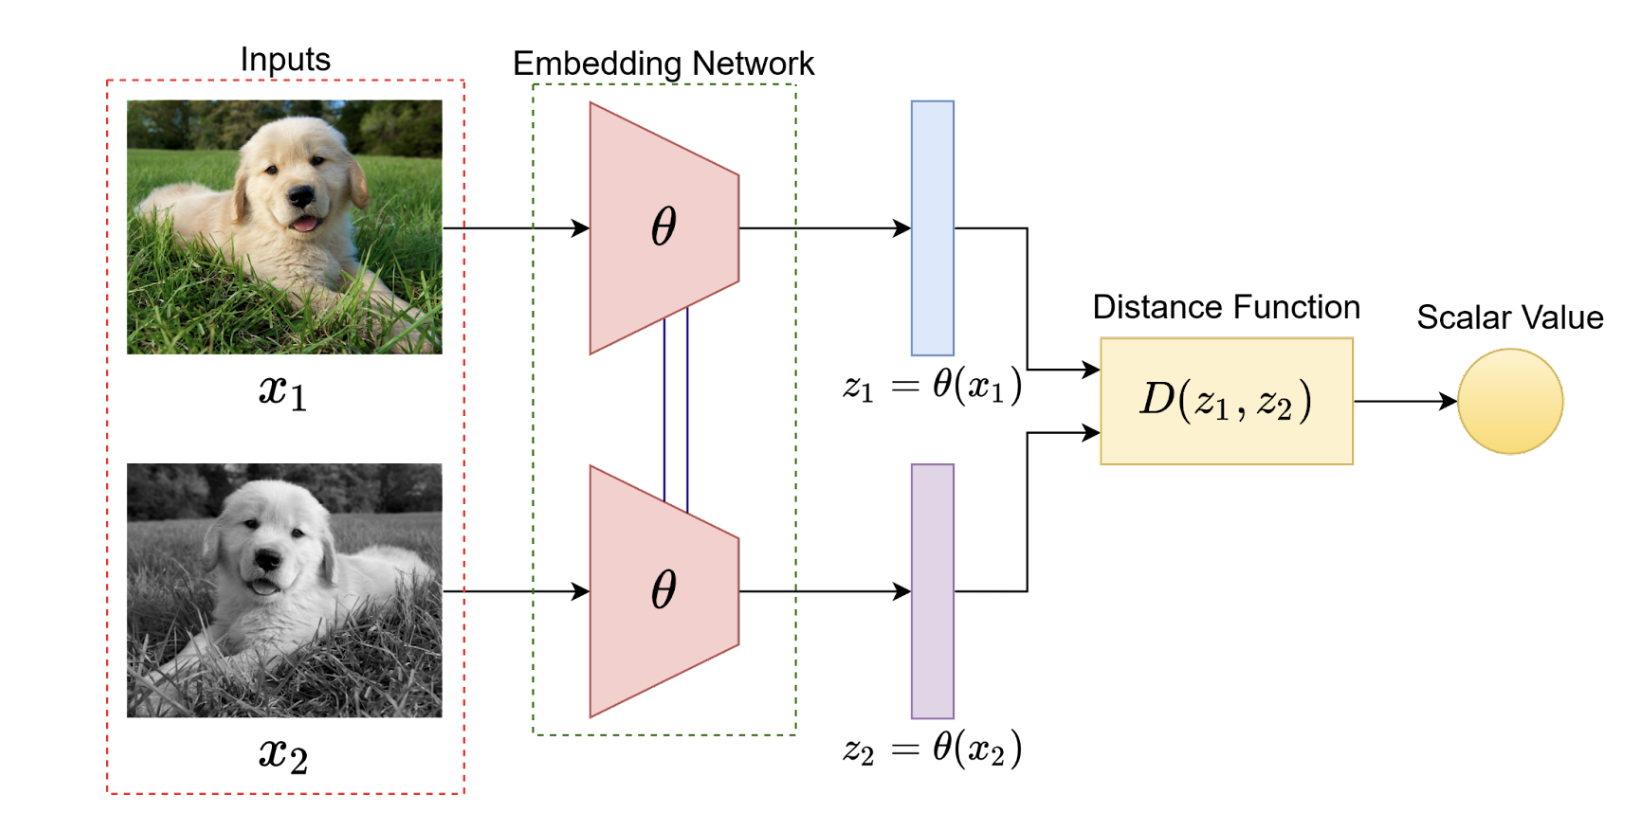
\includegraphics[width=10cm]{dog1.png}
	\captionsetup{font=small} % Adjust the font size of the caption
	\caption{معماری تعبیه مشترک}
	\label{fig:self1}
\end{figure}

\subsection{ الگوریتم‌های متضاد}

الگوریتم‌های متضاد  \LTRfootnote{\lr{Contrastive learning}}‌ با مقایسه و تضاد دیدگاه‌های مختلف از یک داده کار می‌کنند. این مدل آموزش داده شده است تا نقاط داده مشابه را در فضای بازنمایی آموخته شده به هم نزدیک کند در حالی که نقاط داده غیرمشابه را از هم جدا کند. 
%یادگیری متضاد می تواند از فراوانی نمونه های منفی بهره مند شود که به بهبود استحکام مدل کمک می کند.
%این الگوریتم‌ها نیازی به مدل‌سازی مولد صریح ندارند و می‌توانند از نظر محاسباتی کارآمدتر باشند.
هدف الگوریتم‌های متضاد، تضاد دیدگاه‌های مختلف از داده‌های مشابه برای یادگیری نمایش‌های معنادار است. آنها جفت‌های مثبت و منفی نمونه‌های داده را ایجاد می‌کنند و مدل را تشویق می‌کنند تا نمونه‌های مشابه را نزدیک‌تر کند در حالی که نمونه‌های غیرمشابه را در فضای نمایش آموخته‌شده از هم جدا می‌کنند. 
\citep{liu2021self}
در شکل  \ref{fig:self2} دو نمونه از داده مربوط به تصویر سگ به عنوان نمونه مشابه و یک تصویر گربه به عنوان نمونه غیر مشابه در فضای برداری نشان داده شده است که مدل یادگیری متضاد سعی ‌می‌کند فاصله نمونه‌های مشابه را به حداقل و فاصله نمونه‌های غیر مشابه را به حداکثر در فضای برداری برساند.
\citep{falcon2020framework}
% \begin{figure}[htbp]
%	\centering
%	
%\end{figure}

\begin{minipage}{\linewidth}
	\centering
	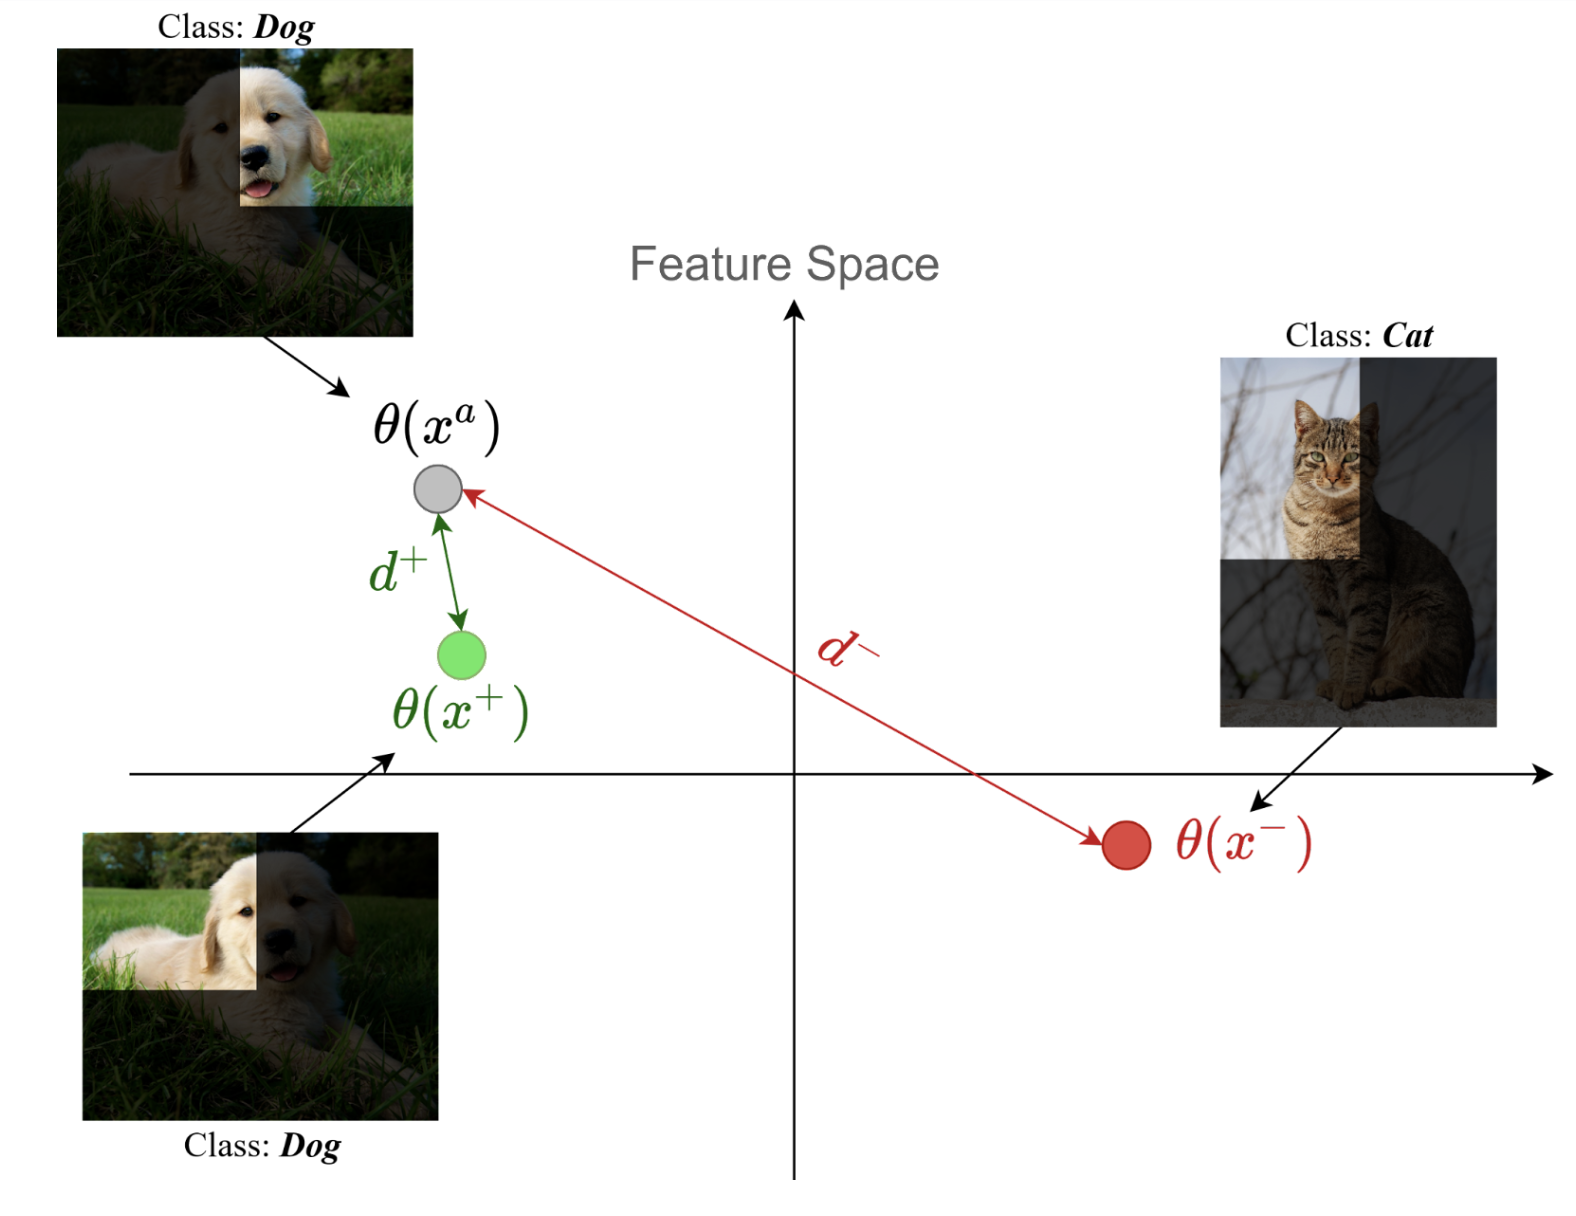
\includegraphics[width=10cm]{dog2.png}
	\captionsetup{font=small} % Adjust the font size of the caption
	\captionof{figure}{الگوریتم یادگیری متضاد}
	\label{fig:self2}
\end{minipage}



\subsection{ روش های تبعیض نمونه}

روش‌های تبعیض نمونه \LTRfootnote{\lr{Instance discrimination method}}‌از ایده کلی یادگیری متضاد، برای کل نمونه‌های داده (مانند یک تصویر کامل) استفاده می کنند.

به عنوان مثال، دو نسخه چرخانده یا برگردان شده از یک تصویر سگ می‌توانند به عنوان جفت  مثبت عمل کنند، در حالی که یک نسخه چرخانده/برگردان شده از یک تصویر گربه می‌تواند به عنوان نمونه منفی باشد. اکنون، مشابه اصل اساسی، فاصله بین جفت مثبت باید به حداقل برسد، در حالی که فاصله بین جفت منفی باید حداکثر شود.

ایده اصلی پشت این تکنیک این است که ورودی, که دستخوش برخی تبدیل‌های داده‌های اساسی شده است باید همچنان از همان دسته باشد، یعنی یک مدل یادگیری عمیق باید نسبت به تبدیل‌ها تغییر ناپذیر باشد. هنگامی که تصویر یک سگ به صورت عمودی چرخانده می‌شود و به مقیاس خاکستری تبدیل می‌شود، همچنان کلاس "سگ" را نشان می دهد.
\citep{taher2022caid}
در این دسته از روش‌ها، یک تصویر تصادفی گرفته می‌شود و تبدیل تصادفی برای ایجاد نمونه مثبت روی آن اعمال می شود (مانند چرخش، برش و غیره). اکنون، چندین تصویر دیگر از مجموعه داده به عنوان نمونه‌های منفی گرفته می شود و یک تابع هزینه طراحی شده است تا فاصله بین جفت‌های نمونه منفی را به حداکثر برساند. شکل \ref{fig:self3}

\begin{minipage}{\linewidth}
	\centering
	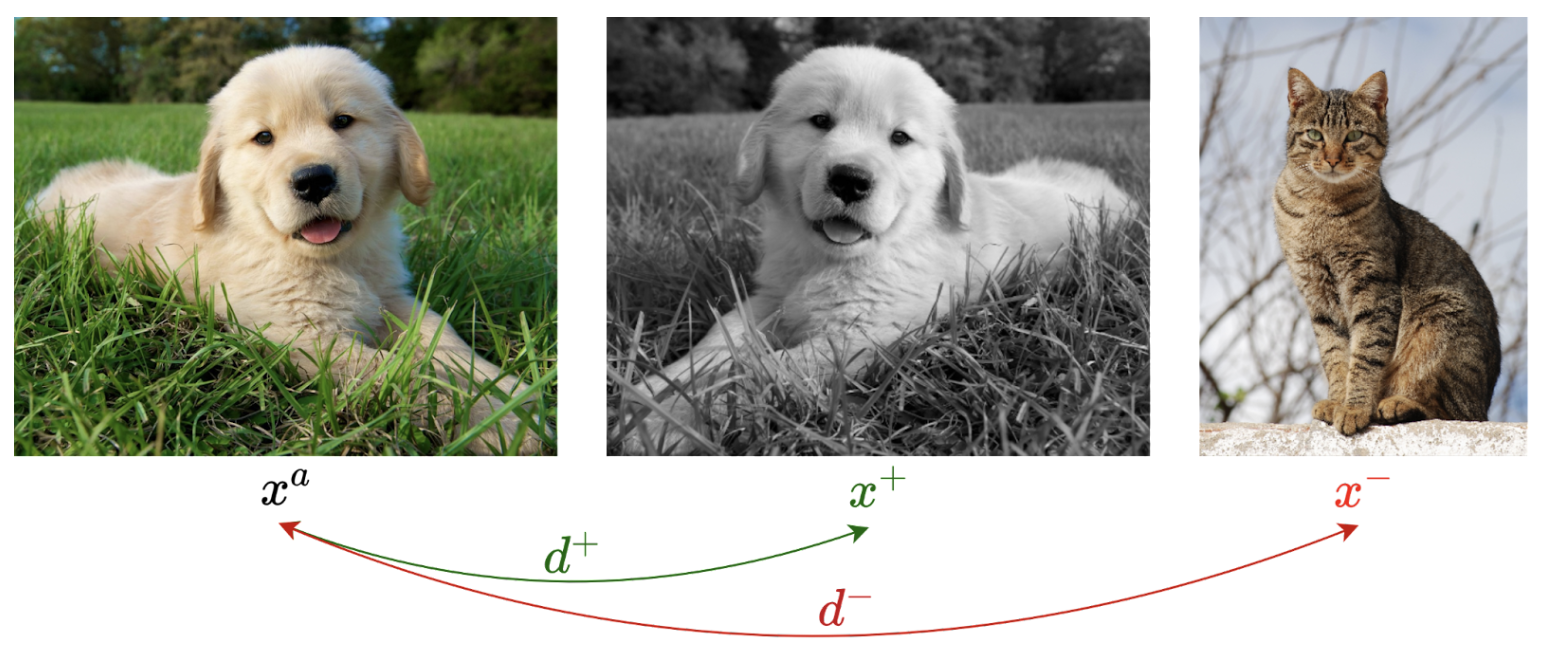
\includegraphics[width=10cm]{dog3.png}
	\captionsetup{font=small} % Adjust the font size of the caption
	\captionof{figure}{روش‌های تبعیض نمونه}
	\label{fig:self3}
\end{minipage}

یکی از روش‌های محبوب در دسته روش‌های تبعیض نمونه الگوریتم یادگیری متضاد ساده\LTRfootnote{\lr{Simplified contrastive learning(simclr)}})  است که در ادامه به توضیح این روش می‌پردازیم


\subsubsection{SimCLR (یادگیری متضاد ساده)}


یک روش یادگیری خود نظارت برای تصاویری است که از یادگیری متضاد برای یادگیری نمایش داده‌ها بدون تکیه بر داده‌های برچسب‌گذاری شده استفاده می‌کنند. این شامل آموزش یک شبکه عصبی برای پیش‌بینی این است که کدام دو تصویر، از یک جفت تصویر، شبیه‌تر هستند. نمایش‌هایی که شبکه یاد می‌گیرد می‌تواند به عنوان جاسازی ویژگی برای کارهای پایین دستی مانند دسته‌بندی تصویر استفاده شود.
\citep{falcon2020framework}
%SimCLR یک چارچوب یادگیری خود نظارت است که توسط Google Research پیشنهاد شده است. این برای یادگیری بازنمایی های بصری قدرتمند با استفاده از یادگیری متضاد طراحی شده است. ایده اصلی پشت SimCLR این است که جفت نماهای تقویت شده مثبت و منفی را از یک نمونه داده ایجاد کند و سپس آنها را در فضای نمایش آموخته شده مقایسه کند.
روش یادگیری متضاد ساده از اجزای کلیدی زیر تشکیل شده است:

1.افزایش داده‌ها\LTRfootnote{\lr{Data augmentation}} : 

هر نمونه ورودی دو بار افزوده می‌شود تا دو نمای متفاوت از یک نقطه داده ایجاد شود.

2.شبکه رمزگذار \LTRfootnote{\lr{Encoder}} : 

یک شبکه عصبی (معمولاً یک شبکه عصبی پیچشی عمیق) برای استخراج ویژگی از نماهای تقویت‌شده داده استفاده می‌شود.

3.سر نمایش دهنده  \LTRfootnote{\lr{Projection head}} :

یک پرسپترون چندلایه \LTRfootnote{\lr{Multilayer preceptron}} با یک لایه پنهان است که فقط بردارهای نمایش را قبل از تابع هزینه کوچک‌تر می‌کند.

4.تابع هزینه متضاد\LTRfootnote{\lr{Contrastive loss function}} : 

هدف مدل این است که نمایش‌های جفت‌های مثبت (نماهای تقویت‌شده همان نمونه) را نزدیک‌تر کند و نمایش‌های جفت‌های منفی (نماهای تقویت‌شده نمونه‌های مختلف) را در فضای ویژگی دورتر کند. تابع هزینه متضاد مدل را تشویق می‌کند تا بازنمایی‌های متمایزکننده‌ای را بیاموزد که ویژگی‌های اساسی داده‌ها را ضبط می‌کند.

در شکل  \ref{fig:self4}  روند کلی الگوریتم یادگیری متضاد ساده نشان داده شده است به این صورت که دو داده افزوده شده به شبکه داده می‌شود و شبکه می آموزد نمایش داده های مربوط به یک کلاس را مشابه هم و نمایش داده‌های کلاس‌های مختلف را متفاوت تولید کند.

\begin{minipage}{\linewidth}
	\centering
	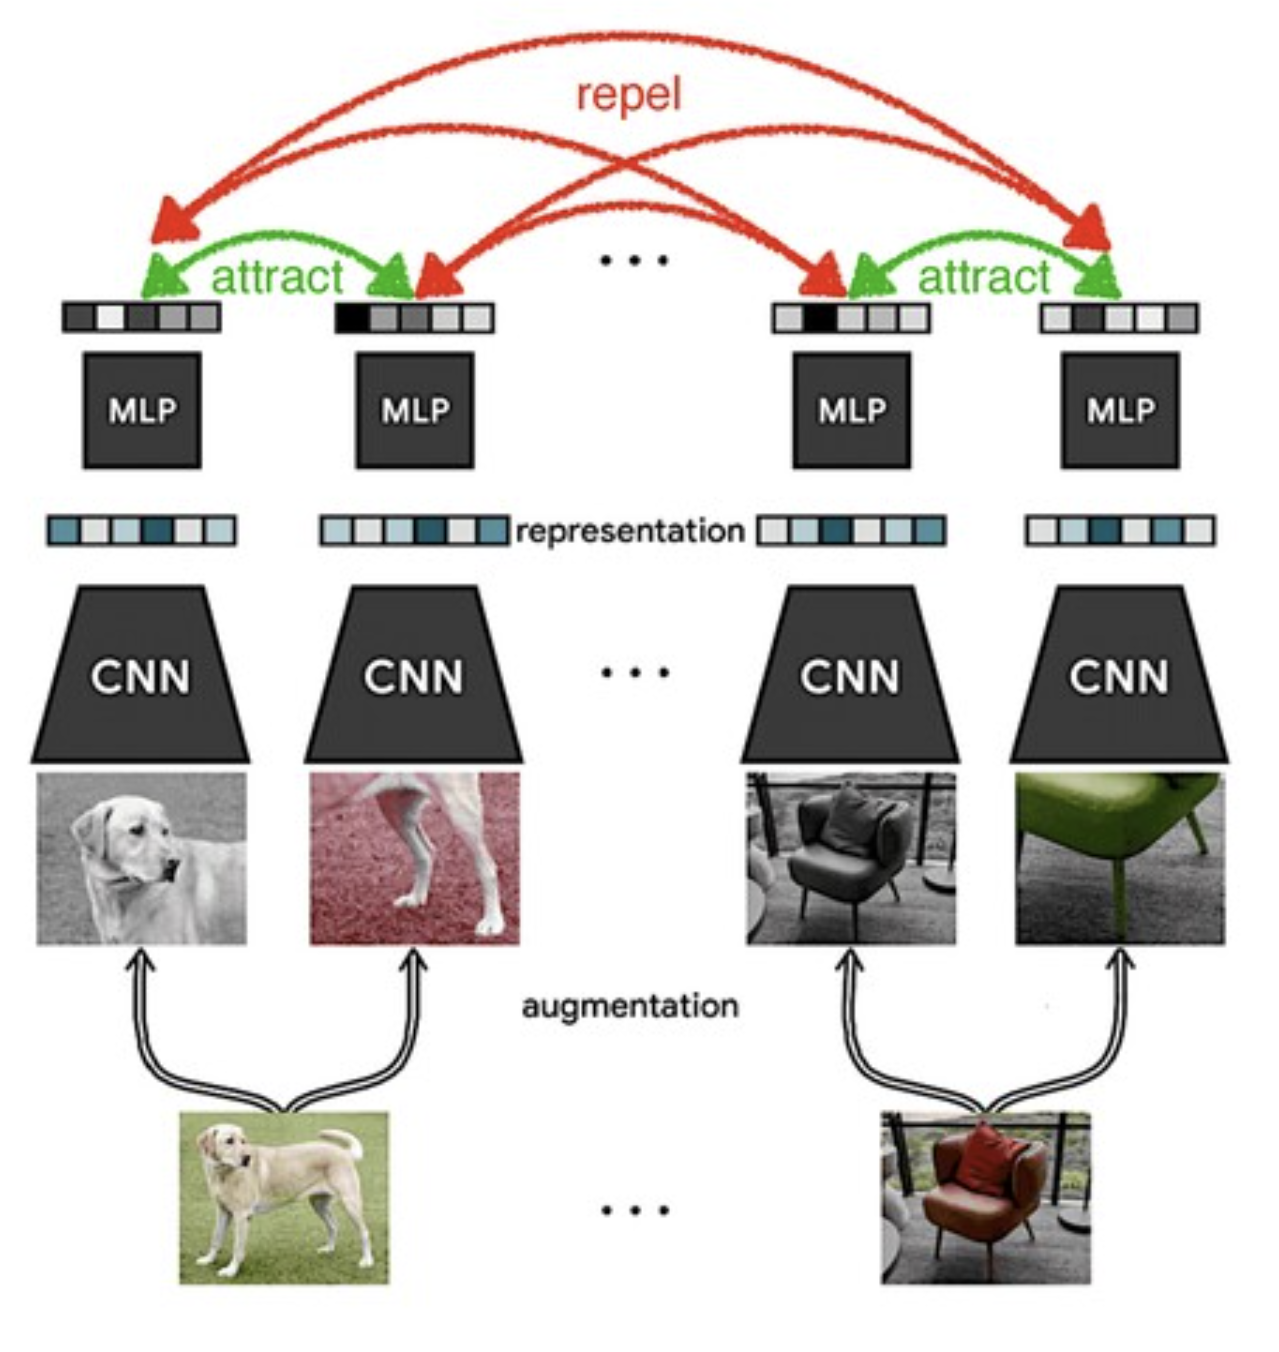
\includegraphics[width=10cm]{dog4.png}
	\captionsetup{font=small} % Adjust the font size of the caption
	\captionof{figure}{روش یادگیری متضاد ساده}
	\label{fig:self4}
\end{minipage}

%\subsubsection{MoCo (مقابل حافظه تقویت شده)}
%MoCo یکی دیگر از چارچوب های یادگیری تحت نظارت خود است که توسط محققان در فیس بوک AI Research (FAIR) معرفی شده است. این نیاز به بانک های حافظه بزرگ برای رسیدگی به تعداد زیادی از نمونه های منفی را برطرف می کند، محدودیتی که الگوریتم های متضاد قبلی با آن مواجه بودند. MoCo از یک بافر حافظه برای ذخیره فرهنگ لغت بزرگی از تعبیه‌های ویژگی استفاده می‌کند که امکان یادگیری متضاد کارآمد با تعداد زیادی نگاتیو را فراهم می‌کند.
%اجزای کلیدی MoCo عبارتند از:
%
%Momentum Update: MoCo یک شبکه رمزگذار مومنتوم را معرفی می کند که میانگین متحرک وزن رمزگذار اصلی است. این امکان نمایش ویژگی های پایدارتر و موثرتر را فراهم می کند.
%Memory Queue: یک بافر حافظه مبتنی بر صف، نمایش نمونه های منفی را ذخیره می کند. در طول آموزش، خروجی رمزگذار در حافظه قرار می‌گیرد و قدیمی‌ترین عناصر صف حذف می‌شوند. این مدل را قادر می سازد تا مجموعه بزرگ و متنوعی از نمونه های منفی را بدون ذخیره صریح آنها حفظ کند.
%هر دو SimCLR و MoCo عملکرد چشمگیری را در وظایف مختلف بینایی کامپیوتری مانند طبقه بندی تصویر، تشخیص اشیا و تقسیم بندی نشان داده اند. این الگوریتم‌های متضاد به طور قابل‌توجهی زمینه یادگیری خود نظارتی را ارتقا داده‌اند و بینش‌های ارزشمندی را برای یادگیری نمایش‌های قدرتمند از داده‌های بدون برچسب به شیوه‌ای بدون نظارت ارائه می‌دهند.

%3. روش های مبتنی بر رمزگذار خودکار:
%رمزگذارهای خودکار شبکه های عصبی هستند که برای بازسازی داده های ورودی از یک نمایش با ابعاد پایین تر (رمزگذار) و سپس بازسازی آن به شکل اصلی (رمزگشا) آموزش دیده اند. رمزگذارهای خودکار با نظارت خود با به حداقل رساندن خطای بازسازی، نمایش های مفیدی را یاد می گیرند.
%
%4. پیش بینی چرخش:
%این روش شامل آموزش مدل برای پیش بینی زاویه چرخش یک تصویر است. با انجام این کار، مدل یاد می‌گیرد که تغییر ناپذیری چرخشی و ویژگی‌های معنادار را ثبت کند.
%
%5. پیش بینی زمینه:
%پیش‌بینی زمینه شامل آموزش مدل برای پیش‌بینی بخش‌های گمشده یا زمینه یک تصویر، اغلب با حذف تکه‌ها یا پوشاندن تصادفی بخش‌هایی از تصویر ورودی است.
%
%6. نمونه تبعیض:
%در این رویکرد، مدل یاد می‌گیرد که با در نظر گرفتن تکنیک‌های افزایش داده‌ها برای ایجاد تغییرات نمونه، بین نمونه‌های مختلف یک کلاس یا شی تمایز قائل شود.

%7. پازل های اره منبت کاری اره مویی:
%پازل‌های اره منبت کاری اره مویی شامل شکستن یک تصویر به چند تکه و به هم ریختن آن‌ها هستند و مدل آموزش داده می‌شود تا با چیدمان صحیح وصله‌ها، معما را حل کند.
%
%8. پیش بینی ترتیب زمانی:
%این روش برای داده های متوالی مانند ویدئو یا صدا استفاده می شود. این مدل برای پیش‌بینی ترتیب زمانی صحیح فریم‌های به هم ریخته یا بخش‌های صوتی آموزش داده شده است.
%
%9. انتساب خوشه:
%انتساب خوشه شامل خوشه بندی نقاط داده در فضای نمایش آموخته شده، تشویق مدل به یادگیری جداسازی موثر خوشه های مختلف است.
%
%اینها تنها نمونه هایی از طیف متنوع الگوریتم های مورد استفاده در یادگیری خود نظارت هستند. هر الگوریتم با چالش ایجاد سیگنال‌های نظارت معنی‌دار از داده‌های بدون برچسب به روش‌های منحصربه‌فردی مقابله می‌کند و کاربردهای آن‌ها به حوزه‌های مختلفی از جمله بینایی رایانه، پردازش زبان طبیعی و تشخیص گفتار گسترش می‌یابد.



\section{روش های افزایش داده و تولید نمونه های جدید}

افزایش داده‌ها \LTRfootnote{\lr{Data augmentation}}یک تکنیک مهم در حوزه یادگیری ماشین است که با استفاده از تغییرات مختلف بر روی داده‌های اصلی، حجم و تنوع مجموعه آموزشی را افزایش می‌دهد. هدف اصلی این تکنیک، کاهش اهمیت بار آموزشی و جلوگیری از بیش‌برازش مدل‌ها به داده‌های آموزشی است. با افزایش تنوع داده‌ها، مدل‌های یادگیری ماشین قادر به بهترین فراگیری الگوها و ویژگی‌ها می‌شوند و در مواجهه با داده‌های جدید و ناشناخته، عملکرد بهتری از خود نشان می‌دهند.
\citep{ng2020ssmba}
افزایش داده‌ها از روش‌های متنوعی مانند تغییرات هندسی، تبدیل‌های رنگی، برش‌ها و چرخش‌ها، نویز اضافه کردن به داده‌ها و... استفاده می‌کند. با اعمال این تغییرات، داده‌ها به شکل مصنوعی تغییر می‌کنند و مجموعه آموزشی با داده‌های جدید و تا حدودی ناشناخته تکمیل می‌شود. این تغییرات همچنین باعث افزایش دقت و پایداری مدل‌ها در مواجهه با شرایط مختلفی می‌شود که ممکن است در داده‌های ورودی واقعی وجود داشته باشند.

در انجام افزایش داده‌ها، اهمیت استفاده از روش‌های مناسب و متعادل برای تغییر داده‌ها وجود دارد. از یک سو، باید مطمئن شویم که داده‌های تغییر یافته معتبر و معنادار هستند و با ویژگی‌های داده‌های اصلی همخوانی دارند. از سوی دیگر، تغییرات اعمال شده نباید اطلاعات اصلی و اساسی داده‌ها را به طور قابل ملاحظه‌ای تغییر دهد تا از از دست دادن اطلاعات مهم جلوگیری شود. به کارگیری تکنیک‌های افزایش داده‌ها باعث بهبود عملکرد و کارایی مدل‌های یادگیری ماشین در حل مسائل مختلف می‌شود و در عمل، جزء مهمی از روش‌های موفق در حوزه یادگیری ماشین به شمار می‌آید.

افزایش داده‌ها  یکی از روش‌های موثر در بهبود عملکرد مدل‌های یادگیری ماشین است. کتابخانه PyTorch ابزارهای متنوعی برای انجام افزایش داده‌ها فراهم می‌کند که به ما اجازه می‌دهد داده‌ها را به صورت مصنوعی تغییر داده و تنوع آن‌ها را افزایش دهیم. در ادامه، به برخی از روش‌های افزایش داده‌ها در PyTorch پرداخته می‌شود:

۱. تغییرات هندسی: این روش‌ها شامل تغییر اندازه، برش، چرخش و انعکاس داده‌ها است. با اعمال این تغییرات، می‌توانیم داده‌ها را به صورت مختلف در فضای هندسی قرار دهیم و از این طریق تنوع مجموعه آموزشی را افزایش دهیم.

۲. تبدیل‌های رنگی: این روش‌ها شامل تغییر رنگ، کنتراست و روشنایی تصاویر است. با اعمال تبدیل‌های رنگی، می‌توانیم داده‌ها را به صورت مصنوعی تغییر رنگ دهیم و با ایجاد تصاویر مختلف، مجموعه آموزشی را متنوع‌ کنیم.

۳. افزودن نویز: با افزودن نویز به داده‌ها، می‌توانیم شباهت آن‌ها را کاهش داده و مدل‌ها را در برابر داده‌های جدید و ناشناخته آماده کنیم. افزودن نویز به تصاویر و ویدئوها از جمله روش‌های متداول این دسته است.


در شکل \ref{fig:self5} نمونه‌هایی از اعمال روش‌های مختلف افزایش داده نشان داده شده است که همانطور که گفته شد برای پیاده سازی الگوریتم‌های یادگیری خودنظارتی به این تکنیک‌های افزایش  داده نیازمند هستیم.

\begin{minipage}{\linewidth}
	\centering
	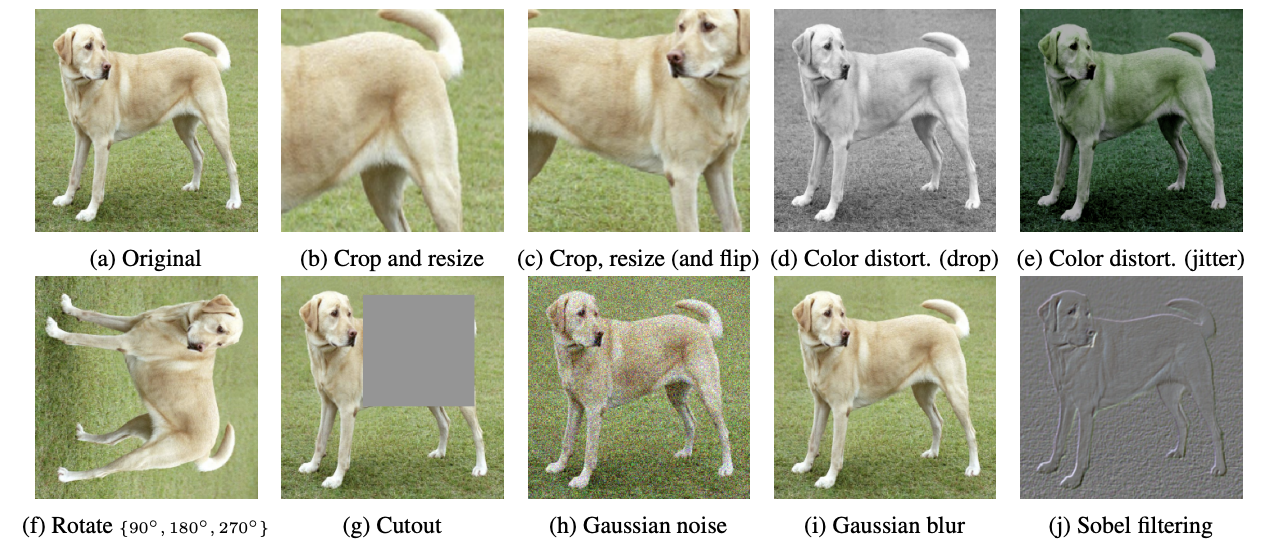
\includegraphics[width=12cm]{dog5.png}
	\captionsetup{font=small} % Adjust the font size of the caption
	\captionof{figure}{روش‌های افزایش داده}
	\label{fig:self5}
\end{minipage}


\section{مفهوم انتقال یادگیری در یادگیری خود نظارتی}

انتقال یادگیری \LTRfootnote{\lr{Transfer learning}} یکی از روش‌های مؤثر در یادگیری خودنظارتی است که به کمک آن می‌توان اطلاعات آموزش‌دیده شده از یک مسئله را به مسئله‌ی دیگری منتقل کرد. در یادگیری خودنظارتی، معمولاً از اطلاعات بدون نظارت در داده‌ها برای آموزش مدل‌ها استفاده می‌شود. اما با انتقال یادگیری، می‌توان از اطلاعات آموزش‌دیده شده در یک مسئله برای حل مسئله‌ی دیگری بهره‌برداری کرد. در شکل \ref{fig:self6} مفهوم انتقال یادگیری در یادگیری ماشین در مقایسه با یادگیری ساده نشان داده شده است.

\begin{minipage}{\linewidth}
	\centering
	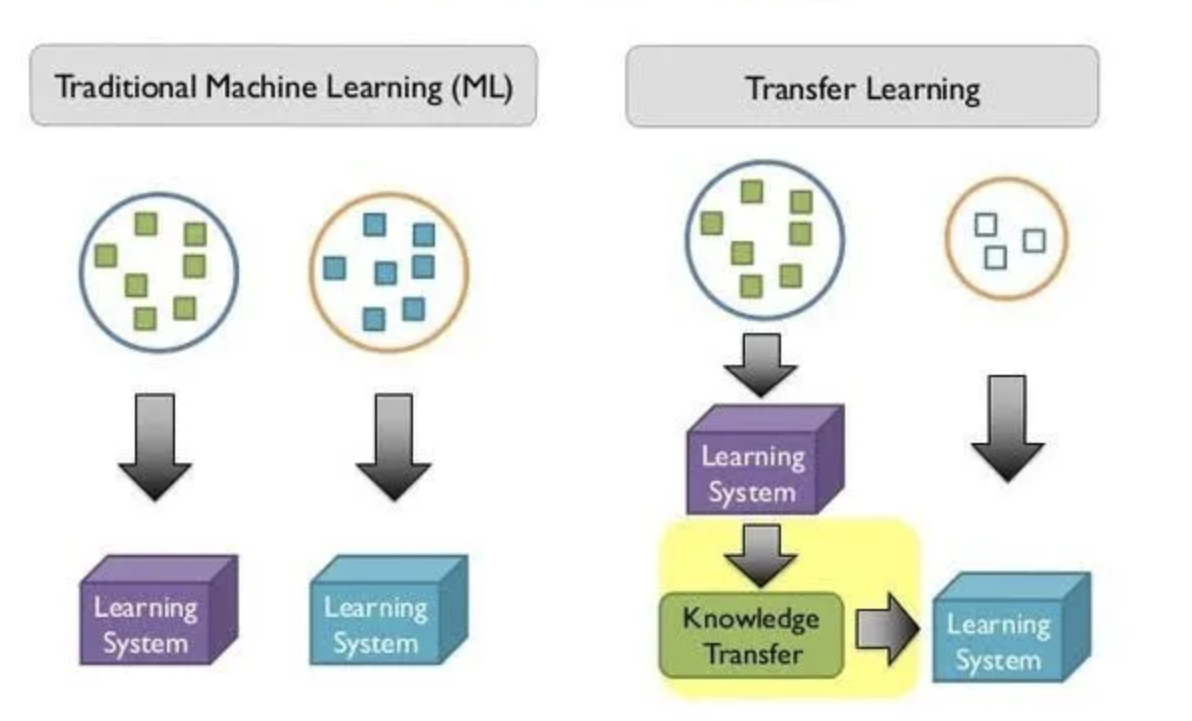
\includegraphics[width=10cm]{self1.png}
	\captionsetup{font=small} % Adjust the font size of the caption
	\captionof{figure}{انتقال یادگیری در مقایسه با یادگیری ساده}
	\label{fig:self6}
\end{minipage}

یکی از روش‌های معمول استفاده از انتقال یادگیری در یادگیری خودنظارتی، استفاده از مدل‌های پیش‌آموزش‌دیده \LTRfootnote{\lr{ Pre-trained models}} است. در این روش، یک مدل با داده‌های بدون برچسب آموزش داده می‌شود. سپس وزن‌های این مدل به عنوان وزن‌های اولیه در حل مسئله‌ی هدف استفاده می‌شود. این انتقال وزن‌ها امکان دسترسی به اطلاعات بدون نظارت از داده‌های پیشین و بهره‌گیری از آن‌ها برای بهبود عملکرد مدل را فراهم می‌کند.
\citep{mao2020survey}
همچنین در انتقال یادگیری در یادگیری خودنظارتی، می‌توان از لایه‌های مشترک میان دو مسئله استفاده کرد. این لایه‌های مشترک می‌توانند اطلاعات کلیدی را که در هر دو مسئله به کار می‌روند، از داده‌های پیشین یاد بگیرند و از آن‌ها برای حل مسئله‌ی هدف استفاده کنند. این روش از نظر محدودیت داده‌ها و منابع محاسباتی مؤثر است و می‌تواند عملکرد مدل‌ها را بهبود بخشد.



تمایز اصلی انتقال یادگیری از یادگیری معمولی این است که در انتقال یادگیری، مدل از داده‌ها و دانش موجود در یک مسئله به مسئله‌ی دیگری منتقل می‌شود. این روش بسیار مؤثر در مواردی است که داده‌های کافی برای آموزش مدل در مسئله‌ی هدف موجود نیست یا هزینه‌ی جمع‌آوری داده‌های جدید بسیار بالاست.

انتقال یادگیری در حوزه‌های مختلفی از جمله بینایی ماشین، پردازش زبان طبیعی، تشخیص الگو و بازیابی اطلاعات استفاده می‌شود و به دلیل کارایی و عملکرد بالا، از محبوبیت بسیاری برخوردار است.
استفاده از انتقال یادگیری در یادگیری خودنظارتی باعث افزایش سرعت آموزش مدل‌ها، بهبود کیفیت نتایج و کاهش نیاز به داده‌های برچسب‌دار می‌شود. در این روش شبکه ابتدا با داده‌های اولیه \LTRfootnote{\lr{Pretext}}بدون برچسب  آموزش می‌بیند سپس شبکه آموزش دیده شده برای حل مساله اصلی با داده‌های برچسب دار استفاده می شود. در شکل \ref{fig:self7} ابتدا شبکه بر روی داده‌های بدون برچسب آموزش می‌بیند و یک نمایش از داده‌ها تولید می‌کند سپس شبکه آموزش دیده شده برای حل یک مساله نظارت شده استفاده می‌شود و در طی یادگیری بر روی داده‌های جدید برچسب دار به  جای از ابتدا آموزش دیدن صرفا تنظیم دقیق \LTRfootnote{\lr{Finetune}}می شود که بسیار سریع و بهینه است.
\citep{medina2020self}

\begin{minipage}{\linewidth}
	\centering
	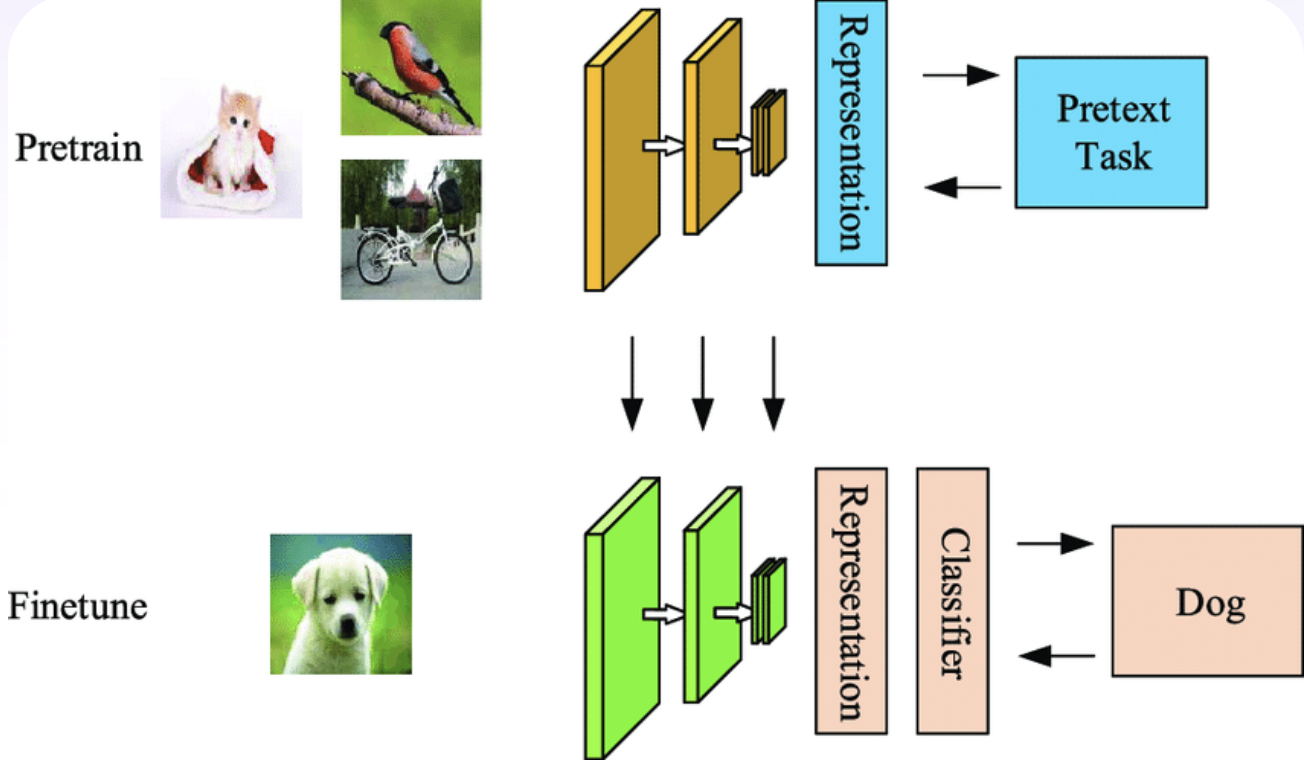
\includegraphics[width=10cm]{self7.png}
	\captionsetup{font=small} % Adjust the font size of the caption
	\captionof{figure}{انتقال یادگیری در فرایند یادگیری خودنظارتی}
	\label{fig:self7}
\end{minipage}


\section{ توابع هزینه در یادگیری خودنظارتی}

در یادگیری خودنظارتی متضاد، تابع خطای مقایسه‌ای برای آموزش مدل به کار می‌رود. هدف اصلی این تابع خطا، ایجاد فضای نمونه در مدل است که نمونه‌های مشابه در این فضا به هم نزدیک شوند، در حالی که نمونه‌های متفاوت از یکدیگر فاصله داشته باشند. با ایجاد این فضای نهان، مدل حساس به تفاوت‌های بین داده‌ها می‌شود و می‌تواند الگوهای مشترک بین داده‌ها را برای تمایز دادن از هم استخراج کند.
\citep{falcon2020framework}
برای تعریف تابع خطا به طور کلی از تابع هزینه رتبه بندی حاشیه  \LTRfootnote{\lr{Margin ranking}}استفاده می‌شود. در این روش، برای هر نمونه اصلی، دو نمونه دیگر انتخاب می‌شوند: یک نمونه مثبت (که مشابه نمونه‌ی اصلی است) و یک نمونه منفی (که با نمونه‌ی اصلی تفاوت دارد). سپس فاصله‌ی نمونه‌ی مثبت از نمونه‌ی اصلی (به عنوان فاصله مثبت) و فاصله‌ی نمونه‌ی منفی از نمونه‌ی اصلی (به عنوان فاصله منفی) محاسبه می‌شود. هدف این تابع خطا، مطمئن شدن از اینکه فاصله‌ی مثبت کمتر از فاصله‌ی منفی باشد و یک حداقل فاصله بین آن‌ها به عنوان لبه وجود داشته باشد. اگر فاصله‌ی مثبت از فاصله‌ی منفی بزرگتر از لبه باشد، تابع خطا مقدار آن را کاهش می‌دهد، در غیر این صورت،  تابع خطا مقدار را افزایش می‌دهد.

در تعریف تابع خطای مقایسه‌ای، می‌توان از انواع مختلفی از فاصله‌ها استفاده کرد، از جمله فاصله اقلیدسی و یا شباهت کسینوسی. همچنین می‌توان مقدار فاصله لبه و انتخاب نمونه‌های مثبت و منفی را به طور دلخواه تنظیم کرد تا بهترین نتایج را بدست آورد.

با استفاده از تابع خطای مقایسه‌ای در یادگیری خودنظارتی متضاد، مدل قادر به استخراج ویژگی‌های معنادار از داده‌ها و یادگیری نمایشی مناسب برای مسائل مختلف خواهد بود. این تابع خطا می‌تواند برای مسائل تشخیص الگو، دسته‌بندی و مدل‌سازی مقایسه‌ای داده‌ها با موفقیت استفاده شود.
\citep{jiao2022timeautoad}
از میان تابع‌های هزینه خودنظارتی، سه تابع رایج عبارتند از:

1. تابع هزینه مقایسه‌ای  \LTRfootnote{\lr{Contrastive Loss}}: 
این تابع برای مسائل مدل‌سازی از نظر مشابهت داده‌ها به کار می‌رود. در این روش، دو نمونه از یک دسته به عنوان ورودی به مدل داده می‌شوند و مدل باید بتواند دو نمونه مشابه را از یکدیگر تشخیص دهد. اگر دو نمونه متفاوت باشند، مدل باید بتواند بین آن‌ها تفاوت را تشخیص دهد. یک فاصله برای لبه در نظر گرفته می شود و با استفاده از محاسبه فاصله اقلیدسی بین نمونه‌های مشابه و غیر مشابه تابع هزینه به صورت زیر تعریف می‌شود :

%\begin{minipage}{\linewidth}
%	\centering
%	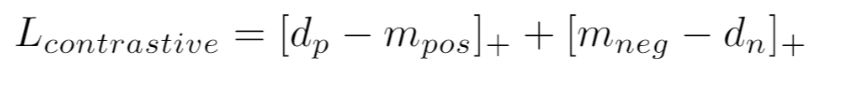
\includegraphics[width=10cm]{loss1.png}
%	%\captionof{figure}{انتقال یادگیری در مقایسه در فرایند یادگیری خودنظارتی}
%	%\label{fig:self7}
%\end{minipage}

\begin{equation}
\mathcal{L}_{\text{contrastive}} = [\text{d}_\text{positive} - \text{m}_\text{positive}] + [\text{m}_\text{negative} - \text{d}_\text{negative}]
\end{equation}




2. تابع هزینه آنتروپی متقاطع با مقیاس دمایی نرمال شده \LTRfootnote{\lr{Normalized Temperature-scaled Cross Entropy }} این تابع برای مسائل تشخیص الگو و مدل‌سازی مقایسه‌ای داده‌ها مورد استفاده قرار می‌گیرد. در این روش، نمونه‌های مختلف از یک دسته با هم مقایسه می‌شوند و مدل باید بتواند نمونه‌های مشابه را از دیگر نمونه‌ها تمایز دهد. تابع ابتدا شباهت کسینوسی یک جفت داده مثبت را محاسبه کرده و سپس آن را تقسیم بر همین مقدار برای کل جفت‌های مثبت در آن دسته داده ‌می‌کند.
\citep{falcon2020framework}

\begin{equation}
	\mathcal{L}_{\text{NTXent}} = -\frac{1}{N} \sum_{i=1}^{N} \log \frac{\exp(\text{sim}(z_i, z_{\text{pos}}) / \tau)}{\sum_{j=1}^{2N} \exp(\text{sim}(z_i, z_j) / \tau)}
\end{equation}


3. تابع هزینه سه‌قلو  \LTRfootnote{\lr{Triplet loss}}: 
این تابع برای مسائل دسته‌بندی و مدل‌سازی مقایسه‌ای داده‌ها مورد استفاده قرار می‌گیرد. به طور کلی مشابه تابع هزینه مقایسه‌ای رفتار می‌کند با این تفاوت که در این روش، سه نمونه از یک دسته به عنوان ورودی به مدل داده می‌شوند: یک نمونه مثبت (که مشابه نمونه‌ی اصلی است)، یک نمونه منفی (که با نمونه‌ی اصلی تفاوت دارد) و نمونه‌ی اصلی. مدل باید بتواند نمونه‌های مشابه را از دیگر نمونه‌ها تمایز دهد و از نمونه منفی فاصله بگیرد. فاصله نمونه‌های مثبت باید برای تمامی نمونه‌ها حداقلی باشد تا مدل به طور کلی درک درستی از دسته‌ها داشته باشد. تابع هزینه سه‌قلو معمولاً از فاصله اقلیدسی یا شباهت کسینوسی رای محاسبه فاصله‌ها استفاده می‌کند. در شکل  \ref{fig:self8}  نحوه محاسبه و عملکرد این تابع هزینه نشان داده‌شده‌است.
\citep{li2022tribyol}
%\begin{minipage}{\linewidth}
%	\centering
%	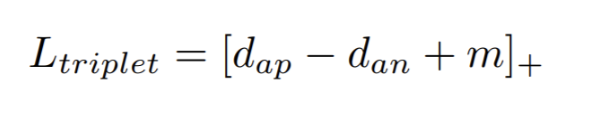
\includegraphics[width=8cm]{loss3.png}
%	%\captionof{figure}{انتقال یادگیری در مقایسه در فرایند یادگیری خودنظارتی}
%	%\label{fig:self7}
%\end{minipage}

\begin{equation}
	L = \max(d(a, p) - d(a, n) + \text{margin}, 0)
\end{equation}

\begin{minipage}{\linewidth}
	\centering
	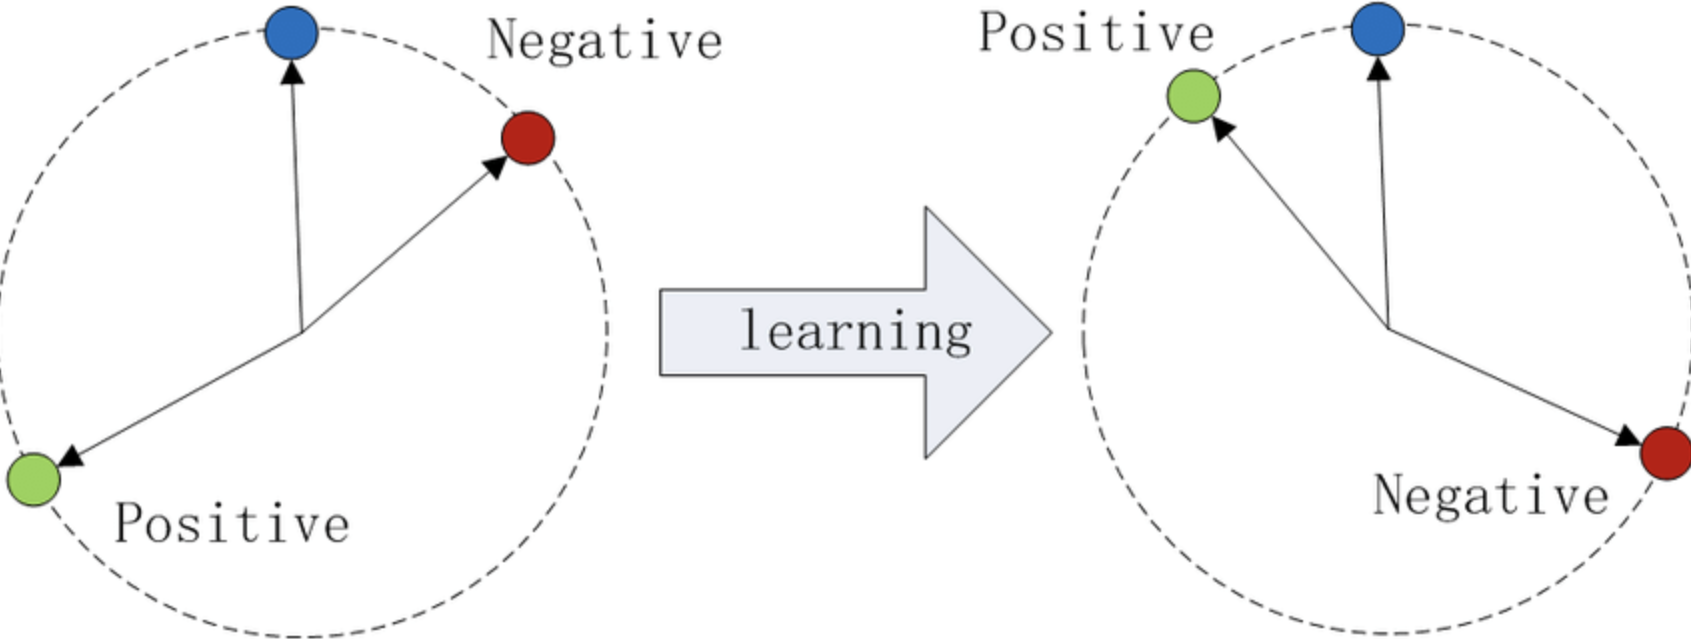
\includegraphics[width=10cm]{loss4.png}
	\captionsetup{font=small} % Adjust the font size of the caption
	\captionof{figure}{عملکرد تابع هزینه سه‌قلو }
	\label{fig:self8}
\end{minipage}



	\clearpage
\phantomsection
%\addcontentsline{toc}{chapter}{مقدمات}
\chapter{تعریف مساله}
\markboth{تعریف مساله}{عنوان فصل}

\section{پیاده سازی روش یادگیری خودنظارتی بر روی شبکه های عصبی ‌اسپایکی}


در این پروژه، قصد داریم از روش یادگیری متضاد ساده استفاده کنیم تا با ترکیب شبکه‌های عصبی اسپایکی با مدل نورونی نشت کننده و ادغام آتش، یادگیری خودنظارتی را بر روی داده‌ها انجام دهیم. از طریق این یادگیری خودنظارتی، قصد داریم نمایش‌های با کیفیتی از داده‌ها استخراج کنیم که می‌توانند در وظایف مختلفی مانند دسته‌بندی استفاده شوند.

با توجه به ماهیت بیولوژیکی شبکه‌های عصبی اسپایکی و پایبند بودن آن‌ها به روش عملکرد نورون‌های واقعی و توانایی در نمایش اطلاعات پردازش شده به صورت الکتریکی و با تولید اسپایک‌ها, استفاده ا این شبکه‌ها این امکان را می‌دهد تا رفتارها و ویژگی‌هایی که در مغز و سیستم عصبی واقعی مشاهده می‌شود را به دقت بیشتری شبیه‌سازی کنیم.
از طرفی بهینه بودن شبکه‌های عصبی اسپایکی در مصرف انرژی و حافظه استفاده از این شبکه‌ها را در حوزه‌های متنوعی به خصوص حوزه‌های سخت‌افزاری نورومورفیک و رباتیک و غیره ممکن ‌می‌سازد.

از سوی دیگر مزیت‌های چشمگیر روش یادگیری خودنظارتی و بی‌نیاز شدن از داده‌های برچسب‌دار برای آموزش شبکه در پیاده‌سازی این روش, با توجه به هزینه‌بر بودن فرایند تولید برچسب و هم‌چنین کمبود داده برچسب‌دار در بسیاری از حوزه‌ها, باعث شد به پیاده‌سازی روش یادگیری خودنظارتی بر روی شبکه‌های عصبی اسپایکی بپردازیم.


به این نتیجه رسیدیم که الگوریتم یادگیری خودنظارتی را بر روی یک شبکه عصبی اسپایکی پیاده‌سازی کنیم و پس از آموزش دیدن شبکه با استفاده از روش انتقال یادگیری، شبکه آموزش دیده را بر روی داده‌های برچسب‌دار برای انجام وظایفی مانند دسته‌بندی نظارت شده آزمایش کنیم.

قبل از اعمال یادگیری خودنظارتی بر روی شبکه‌های عصبی اسپایکی، اقدام به توسعه و افزایش داده‌ها می‌کنیم. این عمل با استفاده از روش‌های افزایش داده مانند چرخش، انتقال، انعکاس و تغییر مقیاس انجام می‌شود. همانطور که در توضیحات روش یادگیری متضاد ساده گفته شده، برای پیاده‌سازی این روش باید از هر داده دو نمونه افزوده شده با یکی از تغییرات گفته شده برای ورودی شبکه تولید کنیم.

پس از انجام افزایش داده، اقدام به اعمال یادگیری خودنظارتی با روش یادگیری متضاد ساده بر روی شبکه می‌کنیم. این روش یادگیری به ما امکان می‌دهد که از معماری‌های پیچیده‌تری برای استخراج نمایندگان با کیفیت از داده‌ها استفاده کنیم. به عبارت دیگر، می‌توانیم اطلاعات کاربردی را از داده‌ها بدون نیاز به برچسب‌های دسته‌بندی شده، استخراج کنیم و از این اطلاعات برای تقویت کارایی شبکه‌های عصبی اسپایکی بهره‌برداری کنیم.

در طی فرآیند یادگیری، هر یک از نمونه‌های افزوده شده به عنوان جریان اسپایکی در گام‌های زمانی به شبکه داده می‌شود و تغییرات پتانسیل نورون‌ها و هم‌چنین آرایه اسپایک‌های خروجی هر نورون در طول زمان به عنوان خروجی شبکه در نظر گرفته می‌شود. با استفاده از توابع هزینه خودنظارتی، شبکه اسپایکی می‌آموزد که برای خروجی جفت‌های مشابه از داده, با الگوی یکسان و برای جفت‌های متفاوت , با الگویی با بیشترین تفاوت اسپایک، خروجی تولید کند.

پس از آموزش شبکه برای ساخت نمایش اسپایکی از هر داده، شبکه آموزش دیده را بر روی داده‌های برچسب‌دار با تعداد کم(۲۰٪ از حجم کل داده) از دو مجموعه MNIST و CIFAR10 منتقل می‌کنیم و میزان عملکرد شبکه را روی مساله دسته‌بندی نظارت شده بررسی می‌کنیم. مشاهده می‌شود نمایش‌های تولید شده توسط شبکه از روی داده‌های بدون برچسب، در حل مساله دسته‌بندی با داده‌های برچسب‌دار با تعداد کم، موثر است و دقت عملکرد شبکه در این مساله بیشتر می‌شود. 
در نتیجه با پیاده‌سازی روش یادگیری خودنظارتی بر روی شبکه‌های عصبی اسپایکی یک ابزار جدید و قدرتمند محاسباتی ساخته می‌شود که از یک سو هزینه برچسب‌ زدن داده را کاهش می‌دهد و نیاز به داده برچسب‌دار برای محاسبه را کم می‌کند و از سوی دیگر با توجه به مزایای شبکه‌های اسپایکی, در حوزه‌های مختلف علوم اعصاب کاربرد بسیاری دارد.

\section{پیشینه تحقیق}

با توجه به نوآورانه بودن این حوزه, تاکنون تحقیقات قبلی در زمینه‌ یادگیری خودنظارتی بر روی شبکه‌های عصبی اسپایکی کمتر متعارف بوده است و اکثر آن‌ها به طور مستقل در یکی از این دو حوزه انجام شده است. با این حال، چندین تلاش پژوهشی در این حوزه به عمل آمده است که می‌توانند به نتایج جالب و مفید منجر شوند.


در یک پژوهش در حوزه تکنولوژی نورومورفیک و شبکه‌های عصبی اسپایکی به بررسی امکانات و پیشرفت‌هایی می‌پردازد که در آن از شبکه‌های عصبی اسپایکی برای انجام وظایف پیچیده‌ای در زمینه بینایی ماشین استفاده می‌شود. این مقاله با بهره‌گیری از شبکه‌های عصبی اسپایکی در یک مسئله پیچیده مانند تخمین جریان نوری نشان می‌دهد که این نوع شبکه‌ها به کمک تصمیم‌گیری خودمتحرک توانسته‌اند عملکرد بهتری در مقایسه با شبکه‌های عصبی معمولی داشته باشند.

یکی از نکات مهم این تحقیق، تلاش برای کاهش نیاز به تطبیق زمانی در ورودی‌های این شبکه‌ها است. به این معنا که شبکه‌های عصبی اسپایکی توانسته‌اند ورودی‌هایی را طراحی کنند که بدون نیاز به اطلاعات زمانی دقیق، عملکرد خوبی در مواجهه با داده‌های پویا و بدون ساختار داشته باشند. این مسئله بسیار مهم است چرا که در بسیاری از موارد در بینایی ماشین، داده‌ها به صورت زمانی تغییر می‌کنند و این توانایی بدون نیاز به تطبیق زمانی می‌تواند عملکرد سیستم را بهبود بخشد.
در شکل \ref{fig:rel1}  ایده کلی پیاده‌سازی انجام شده قابل مشاهده است.

\begin{minipage}{\linewidth}
	\centering
	\includegraphics[width=10cm]{rel1.png}
	\captionsetup{font=small} % Adjust the font size of the caption
	\captionof{figure}{تخمین جریان نوری بر مبنای واقعه‌های خودآموز برای شبکه‌های عصبی اسپایکی عمیق. جریان واقعه به بخش‌های کوچک با تعداد یکسانی از واقعه‌ها تقسیم می‌شود، سپس به شکل مناسبی قالب‌بندی می‌شود و سپس به ترتیب به شبکه وارد می‌شود. برای هر بخش، نقشه جریان نوری پیش‌بینی می‌شود که هر واقعه ورودی را با یک بردار حرکت مرتبط می‌کند. هنگامی که تعداد کافی از واقعه‌ها پردازش شده باشد، با استفاده از تابع هزینه متضاد یک مرحله یادگیری انجام می‌شود..}
	\label{fig:rel1}
\end{minipage}




دریک تحقیق دیگر, تخمین جریان نوری براساس داده‌های واقعه‌ای با شبکه‌های عصبی اسپایکی به بررسی استفاده از دوربین‌های مبتنی بر واقعه \LTRfootnote{\lr{Event-based}} برای وظایفی مانند تشخیص حرکت با سرعت بالا و ملاحظه در محیط‌های کم نور که دوربین‌های معمولی در آن‌ها با مشکلات مواجه می‌شوند، می‌پردازد. این توانایی به دلیل داشتن وضوح زمانی بالا، دامنه پویایی بالا و مصرف انرژی پایین این دوربین‌ها امکان‌پذیر می‌شود. با این حال، روش‌های بینایی ماشین معمولی و شبکه‌های عصبی مصنوعی عمیق مناسب برای کار با خروجی‌های ناهمگام و گسسته دوربین مبتنی بر واقعه نیستند. شبکه‌های عصبی اسپایکی به عنوان شبکه‌های مناسبی برای کار با خروجی‌های دوربین مبتنی بر واقعه عمل می‌کنند، اما این شبکه‌ها به تنهایی  به دلیل پدیده ناپدید شدن اسپایک‌ها در لایه‌های عمیق عملکرد مطلوبی ندارند.

برای حل این مشکلات، در این مقاله یک مدل ارائه شده است، که یک معماری شبکه عصبی هیبریدی عمیق است که شبکه‌های عصبی معمولی را با شبکه‌های عصبی اسپایکی به صورت یکپارچه ترکیب می‌کند تا به بهترین شکل ممکن از خروجی‌های دوربین مبتنی بر واقعه برای تخمین جریان نوری بهره ببرد، در حالی که کارایی را حفظ می‌کند.
 این شبکه با یادگیری خودنظارتی ر روی یک مجموعه داده آموزش داده شده و در پیش‌بینی جریان نوری عملکرد بهتری نسبت به مدل‌های شبکه‌های عصبی معمولی دارد و همچنین کارایی محاسباتی قابل توجهی را فراهم می‌کند. در شکل \ref{fig:rel2} معماری ایده پرداخته شده در پژوهش نشان داده‌شده است.


\begin{minipage}{\linewidth}
	\centering
	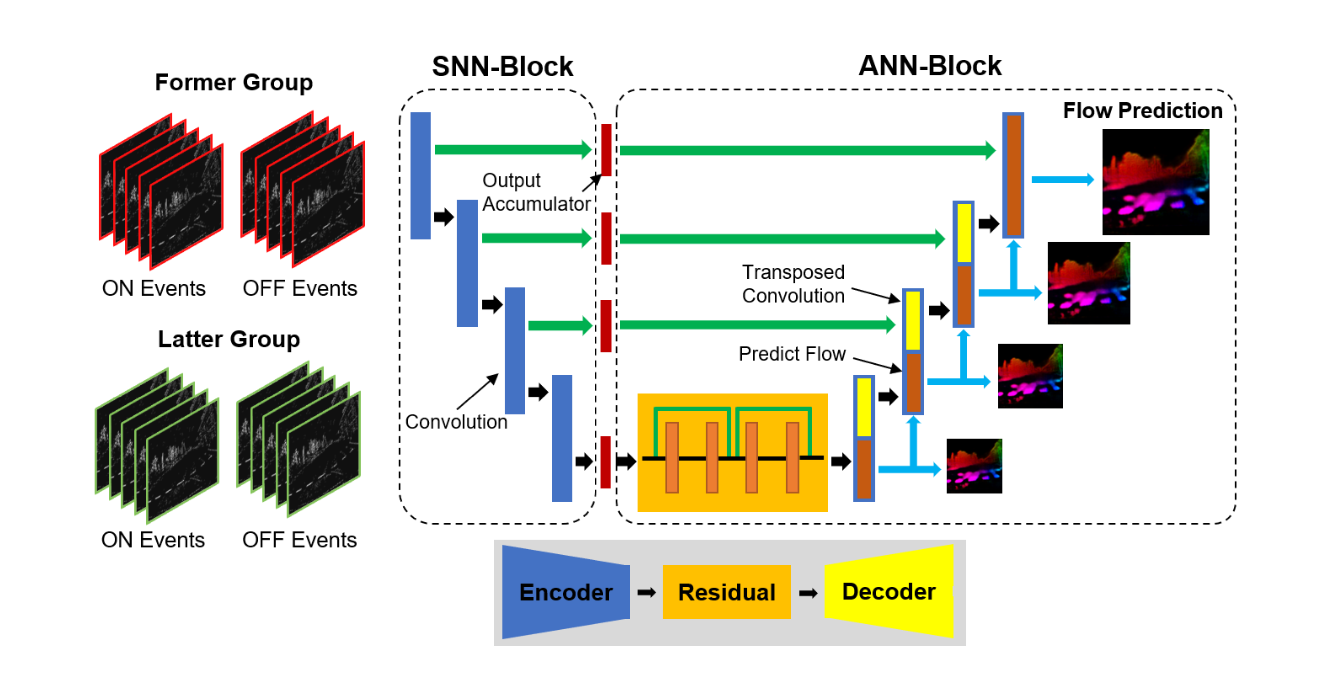
\includegraphics[width=10cm]{rel2.png}
	\captionsetup{font=small} % Adjust the font size of the caption
	\captionof{figure}{معماری شبکه ساخته شده :
		تصاویر ورودی با چهار کانال، به ترتیب از طریق شبکه هیبریدی عبور می‌کنند. بلوک اسپایکی شامل لایه‌های ورودی و سپس تجمع خروجی است، در حالی که بلوک شبکه عصبی مصنوعی شامل لایه‌های باقی‌مانده است. پس از انتقال همه چارچوب‌های واقعه ورودی پشت‌سرهم در داخل پنجره زمانی، تابع خطا ارزیابی می‌شود و روند یادگیری طی می‌شود.}
	\label{fig:rel2}
\end{minipage}





به طور کلی، تاکنون تحقیقات انجام شده در حوزه‌ یادگیری خودنظارتی بر روی شبکه‌های عصبی اسپایکی اثبات می‌کند که این روش‌ها می‌توانند به عنوان یک راهکار موثر برای بهبود عملکرد شبکه‌ها در وظایف مختلف مورد استفاده قرار گیرند. همچنین، این تحقیقات نشان می‌دهد که استفاده از دانش به‌دست‌آمده از مسائل خودنظارتی می‌تواند در تسریع یادگیری و بهبود کیفیت نمایش‌ها بسیار مؤثر باشد و پیاده‌سازی این روش‌ بر روی شبکه‌های عصبی اسپایکی با توجه به بهینه بودن و ساختار این شبکه‌ها می‌تواند در حوزه‌های مختلف بینایی ماشین نقش مهمی را ایفا کند.


\section{چالش‌ها}

چالش‌ها و مشکلاتی که در پیاده‌سازی یادگیری خودنظارتی بر روی شبکه‌های عصبی سنگین اسپایکی وجود دارند می‌توانند به شکل زیر باشند:


بالاخره، این چالش‌ها در پیاده‌سازی یادگیری خودنظارتی بر شبکه‌های عصبی سنگین اسپایکی می‌توانند به شرح زیر توضیح داده شوند:

1. نرخ اسپایک‌ها: 

در شبکه‌های عصبی اسپایکی، اطلاعات به صورت گسسته و در قالب اسپایک‌ها منتقل می‌شوند. این معمولاً به معنای این است که اطلاعاتی تنها در زمان وقوع یک اسپایک متنقل می‌شوند. بنابراین، تعیین کردن کیفیت و اهمیت این اسپایک‌ها و همچنین انتخاب زمان مناسب برای آنها می‌تواند چالش‌هایی ایجاد کند.

2. انتخاب تابع هزینه:

 انتخاب یک تابع هزینه مناسب در یادگیری خودنظارتی مهم است. این تابع باید بتواند اطلاعات مهم و قابل استفاده را از داده‌ها استخراج کند و در طی فرآیند یادگیری نمایش‌های مناسبی از داده بسازد به این صورت که نمایش‌های مربوط به یک داده افزوده شده بیشترین شباهت و با نمایش دیگر داده‌ها بیشترین تفاوت را داشته باشد. 

3. پیچیدگی محاسباتی: 

یادگیری خودنظارتی معمولاً نیازمند محاسبات پیچیده‌ای است و این محاسبات ممکن است نیاز به توانایی‌های محاسباتی قوی در سخت‌افزار داشته باشد. بنابراین، سخت‌افزارها باید مناسب برای انجام این محاسبات باشند و ممکن است فرآیند یادگیری زمان‌بر باشد.

4. دقت پایین: 

یادگیری خودنظارتی معمولاً روی داده‌های بدون برچسب انجام می‌شود و این می‌تواند به دقت پایین‌تری در مدل‌های یادگیری خودنظارتی منجر شود. این دقت پایین ممکن است چالش بزرگی را در مسائلی مانند تشخیص اشیا یا تصویربرداری از رخدادها ایجاد کند.


با توجه به نوآورانه بودن این حوزه، وجود چالش در محاسبات و پیاده‌سازی امری طبیعی است و به پشتکار و تلاش مداوم برای حاصل شدن پیشرفت نیاز دارد. در این تحقیق تلاش نموده‌ایم با پیاده‌سازی روش یادگیری خودنظارتی بر روی یک شبکه عمیق اسپایکی با چالش‌ها روبه‌رو شویم و یک نوآوری در این حوزه انجام داده و یک ابزار مفید برای انجام وظایف مختلف در حوزه یادگیری ماشین بسازیم.

	\clearpage
\phantomsection
%\addcontentsline{toc}{chapter}{مقدمات}
\chapter{روش پیشنهادی}
\markboth{روش پیشنهادی}{عنوان فصل}
\section{آماده سازی داده ورودی}


مجموعه داده‌های MNIST\LTRfootnote{\lr{Modified National Institute of Standards and Technology database
}} و CIFAR-10 \LTRfootnote{\lr{Canadian Institute For Advanced Research}}‌ دو مجموعه داده معروف و پرکاربرد در حوزه تشخیص الگو هستند که به عنوان محیط‌های آزمایشی برای بسیاری از مدل‌ها و الگوریتم‌های یادگیری عمیق استفاده می‌شوند.

\subsection{ مجموعه داده MNIST}



این مجموعه داده شامل تصاویر دست‌نویسی از ارقام از ۰ تا ۹ است که به صورت ۲۸در۲۸ پیکسل و به صورت خاکستری نمایش داده می‌شوند. مجموعه داده MNIST به عنوان یک مجموعه آموزشی کلاسیک در تشخیص ارقام مورد استفاده قرار می‌گیرد و بسیاری از مدل‌های یادگیری عمیق از جمله شبکه‌های عصبی پیچشی  \LTRfootnote{\lr{ Convolutional neural network}}و  شبکه‌های عصبی بازگشتی {\large {\normalsize {\large \LTRfootnote{\lr{Recurrent neural network}}}}} بر روی آن آموزش می‌بینند. در این پروژه از این مجموعه داده برای آزمون میزان یادگیری خودنظارتی در شبکه عصبی اسپایکی استفاده شده است. در شکل  \ref{fig:data1}یک نمونه از مجموعه داده MNIST نشان داده شده است.

\begin{minipage}{\linewidth}
	\centering
	\includegraphics[width=10cm]{mnist.png}
	\captionsetup{font=small} % Adjust the font size of the caption
	\captionof{figure}{نمونه مجموعه داده MNIST}
	\label{fig:data1}
\end{minipage}

\subsection{ مجموعه داده CIFAR10}


مجموعه داده CIFAR10 شامل تصاویر رنگی از ده کلاس مختلف از اشیاء مختلف است. هر تصویر از این مجموعه داده ابعادی به اندازه ۳۲در۳۲ پیکسل و سه کانال رنگی (قرمز، سبز، آبی) دارد. این مجموعه داده به عنوان یک مجموعه آموزشی و ارزیابی محبوب در حوزه تشخیص الگو، تصویربرداری، و بینایی ماشین استفاده می‌شود. شبکه‌های عصبی پیچشی به خوبی برای طبقه‌بندی تصاویر در این مجموعه داده مورد استفاده قرار می‌گیرند . در این پروژه از این مجموعه داده به عنوان داده مورد تایید  برای سنجش کارآیی مدل ساخته شده با شبکه عصبی اسپایکی‌ استفاده می‌شود. در شکل \ref{fig:data2} یک نمونه از مجموعه داده CIFAR10 قابل مشاهده است.



\begin{minipage}{\linewidth}
	\centering
	\includegraphics[width=10cm]{cifar.png}
	\captionsetup{font=small} % Adjust the font size of the caption
	\captionof{figure}{نمونه مجموعه داده CIFAR10}
	\label{fig:data2}
\end{minipage}


این دو مجموعه داده از مجموعه داده‌های کلاسیک برای آموزش و ارزیابی مدل‌های یادگیری عمیق به شمار می‌آیند و با توجه به سادگی و قدرت تشخیصی‌شان، همچنان در مطالعات بسیاری از پژوهش‌های مرتبط با هوش مصنوعی و یادگیری ماشین مورد استفاده قرار می‌گیرند.

\subsection{افزایش داده}
برای استفاده از داده‌های مجموعه‌های MNIST و CIFAR10 در یادگیری خودنظارتی، افزایش حجم داده‌ها از اهمیت بسیاری برخوردار است. با اعمال تکنیک‌های مختلف افزایش حجم داده به داده‌های آموزشی، می‌توان تنوع بیشتری ایجاد کرد و عملکرد مدل‌ها را بهبود بخشید.

۱. چرخش\LTRfootnote{\lr{Rotation}} : 

با اعمال چرخش‌های مختلف به تصاویر، امکان ایجاد تصاویری با زوایای مختلف به وجود می‌آید. این تغییرات می‌تواند به مدل‌ها کمک کند تا به الگوها و تفاوت‌هایی که در زوایای مختلف وجود دارد، حساس‌تر شوند.

۲. برش \LTRfootnote{\lr{Crop}}:

 با برش بخش‌های تصاویر اصلی، می‌توان تصاویر جدید با ابعاد مختلف و محتواهای مختلف ایجاد کرد. این تغییرات به افزایش تنوع داده‌ها کمک می‌کند و می‌تواند اثرات مثبتی در یادگیری مدل‌ها داشته باشد.

۳. مات \LTRfootnote{\lr{Gaussian Blur}} :

 اعمال اثر مات به تصاویر می‌تواند جزئیات غیرضروری را حذف کند و برای مدل‌ها کار کردن با داده‌های نویزی را آموزش دهد. این تغییرات می‌تواند مدل‌ها را به صورت مستقل از تفاوت‌های جزئی در داده‌ها آموزش دهد.

۴. وارونه \LTRfootnote{\lr{Flip}} :

انعکاس تصاویر از روش‌های ساده و موثر برای افزایش حجم داده‌هاست. با اعمال این تغییر، تصاویر جدید با جهت‌های مختلف ایجاد می‌شوند که به مدل‌ها کمک می‌کند تا به الگوها و تفاوت‌های جهتی حساس‌تر شوند.

با اعمال این تغییرات به داده‌های MNIST و CIFAR10، می‌توان تعداد زیادی داده‌آموزشی جدید ایجاد کرد و مدل‌ها را با داده‌های متنوعی آموزش داد. این تنوع می‌تواند به افزایش دقت و کارایی مدل‌ها در مراحل بعدی یادگیری کمک کند و عملکرد آن‌ها را بهبود بخشد. با استفاده از داده‌های افزایش‌یافته, می‌توان به بهبود عملکرد یادگیری خودنظارتی بر روی شبکه‌های عصبی اسپایکی با اجرای الگوریتم‌های پیچیده‌تری در مراحل بعدی پرداخت. در این پروژه با استفاده از روش‌های مختلف افزودن داده روند یادگیری خودنظارتی شبکه عصبی اسپایکی را مورد بررسی قرار دادیم. در شکل\ref{fig:data4}  پیاده سازی روش‌های مختلف افزایش داده  بر روی داده‌های MNIST  و  CIFAR10 قابل مشاهده است.

\begin{minipage}{\linewidth}
	\centering
	\includegraphics[width=10cm]{mnist2.png}
	%\captionof{figure}{نمونه مجموعه داده MNIST}
	\label{fig:data3}
\end{minipage}

\begin{minipage}{\linewidth}
	\centering
	\includegraphics[width=10cm]{cifar2.png}
	\captionsetup{font=small} % Adjust the font size of the caption
	\captionof{figure}{  روش های افزودن داده . به ترتیب روش های مات, چرخش , وارون افقی و برش پیاده‌سازی شده‌است. }
	\label{fig:data4}
\end{minipage}



\section{ساخت معماری شبکه}

 در ساخت شبکه عصبی اسپایکی برای مدلسازی نورون نشت کننده و ادغام آتش از پکیج snntorch \LTRfootnote{\lr{https://snntorch.readthedocs.io/en/latest/index.html}} استفاده شده و  پیاده سازی اتصالات بین نورون ها به وسیله pytorch انجام شده است.
 هر نورون در مدل نورونی snntorch.leaky یک پارامتر به عنوان جریان و یک پارامتر به عنوان پتانسیل گام زمانی قبلی دریافت می‌کند و دو لیست با عنوان‌های اسپایک تولید شده توسط نورون(اگر پتانسیل از آستانه عبور کند برابر با یک و در غیر این صورت برابر با صفر خواهد بود.) و پتانسیل گام زمانی فعلی نورون را به عنوان خروجی می‌دهد. 
 \citep{eshraghian2021training}
 
 با توجه به اینکه مفهوم زمان در شبکه‌های عصبی اسپایکی مورد توجه است و داده‌ها در طول زمان به صورت جریان ثابت وارد شبکه شده و فرآیند تغییر پتانسیل و تولید اسپایک نیز در طول زمان اتفاق می افتد, خروجی مدل نورونی یک بعد زمان نیز دارد و داده‌ها که به صورت فریم‌های عکس در قالب جریان به نورون‌ها وارد می‌شوند در طول چند گام زمانی چندین بار وارد شبکه شده و تغییرات پتانسیل و گسیل اسپایک از نورون در گام‌های زمانی ضبط می‌شود.
 ساختار خروجی نورون‌ها به صورت :
\[
\left[ \text{step time} \times \text{ size batch} \times \text{ dimension feature} \right]
\]
 
 خواهد بود. در فرایند آموزش شبکه تابع هزینه را برای خروجی هر یک از نورون‌ها در تمام گام‌های زمانی محاسبه کرده و در نهایت مجموع آن را به عنوان مقدار هزینه در نظر می‌گیریم و سعی در کمینه کردن آن داریم.
 
  برای اتصالات بین نورون‌ها از لایه‌های پیچشی و همچنین از لایه‌های کاملا متصل استفاده کرده‌ایم. با توجه به اینکه معماری‌های شبکه‌های عصبی پیچشی برای یادگیری خودنظارتی مناسب هستند معماری شبکه عصبی اسپایکی را با الهام از شبکه‌های پیچشی پیاده‌سازی کرده و مدل نورونی را نشت کننده و ادغام آتش قرار دادیم.

در ادامه به توضیح بیشتر معماری مدل نورونی و اتصال لایه‌ها در شبکه می‌پردازیم :

لایه‌های پیچشی \LTRfootnote{\lr{Convolutional layers}}:

شبکه با یک سری لایه‌ پیچشی شروع می‌شود. این لایه‌ها عملیات پیچش دو بعدی را روی داده‌های ورودی انجام می دهند. این لایه‌ها به گونه‌ای طراحی شده‌اند که با اعمال مجموعه‌ای از فیلترهای قابل یادگیری (هسته‌ها\LTRfootnote{\lr{Kernel}}) ویژگی‌ها را در تصاویر ورودی ثبت کنند. این فیلترها روی تصویر می لغزند و نقشه‌های ویژگی را تولید می کنند که جنبه‌های مختلف ورودی را برجسته می کند.
\citep{o2015introduction}

لایه‌های عصبی نشت کننده و ادغام آتش :(LIF)

بعد از هر لایه پیچشی، یک لایه نورون نشت‌کننده و ادغام و آتش (LIF) مربوطه اعمال می شود. این لایه‌ها مدل نورون LIF را پیاده‌سازی می‌کنند. نورون‌های LIF رفتار نورون‌های واقعی را با ادغام اسپایک‌های ورودی در طول زمان شبیه سازی می کنند. اگر پتانسیل غشای یکپارچه از یک آستانه خاص فراتر رود، نورون یک اسپایک خروجی ساطع می کند. مدل LIF یک پارامتر نشتی را نیز معرفی می‌کند که کاهش تدریجی پتانسیل غشا را در طول زمان نشان می‌دهد.


حداکثر ادغام \LTRfootnote{\lr{Max-pooling}}:

در سراسر شبکه، لایه‌های حداکثر ادغام پس از لایه‌های پیچشی و LIF اعمال می‌شوند. این لایه‌ها نقشه‌های ویژگی به‌دست‌آمده از لایه‌های قبلی را پایین می‌آورد و ابعاد فضایی آن‌ها را کاهش می‌دهد. این عملیات به استخراج ویژگی‌های کلیدی از داده‌ها کمک می‌کند و در عین حال پیچیدگی محاسباتی را کاهش می‌دهد.


لایه‌های کاملا متصل\LTRfootnote{\lr{Fully connected}}:

در انتهای شبکه، از لایه‌های کاملاً متصل برای کاهش بعد نقشه‌های ویژگی به‌دست‌آمده از لایه‌های قبلی و تبدیل آن‌ها به یک بردار تک بعدی استفاده می‌شود. این لایه‌ها تبدیل‌های خطی روی داده‌ها انجام می‌دهند. لایه‌های نورون LIF مشابه لایه‌های قبلی بعد از لایه‌های کاملا متصل نیز اعمال می‌شوند.

در شکل  \ref{fig:arc} یک نمونه از نوع اتصالات لایه‌ها در شبکه نشان داده‌شده است. لازم به ذکر است لایه‌های نورونی اسپایکی در بین هریک از اتصالات شبکه قرار گرفته و خروجی اسپایکی نورون‌ها به وسیله اتصالات در شبکه فرآیند یادگیری را طی می‌کنند.

\begin{minipage}{\linewidth}
	\centering
	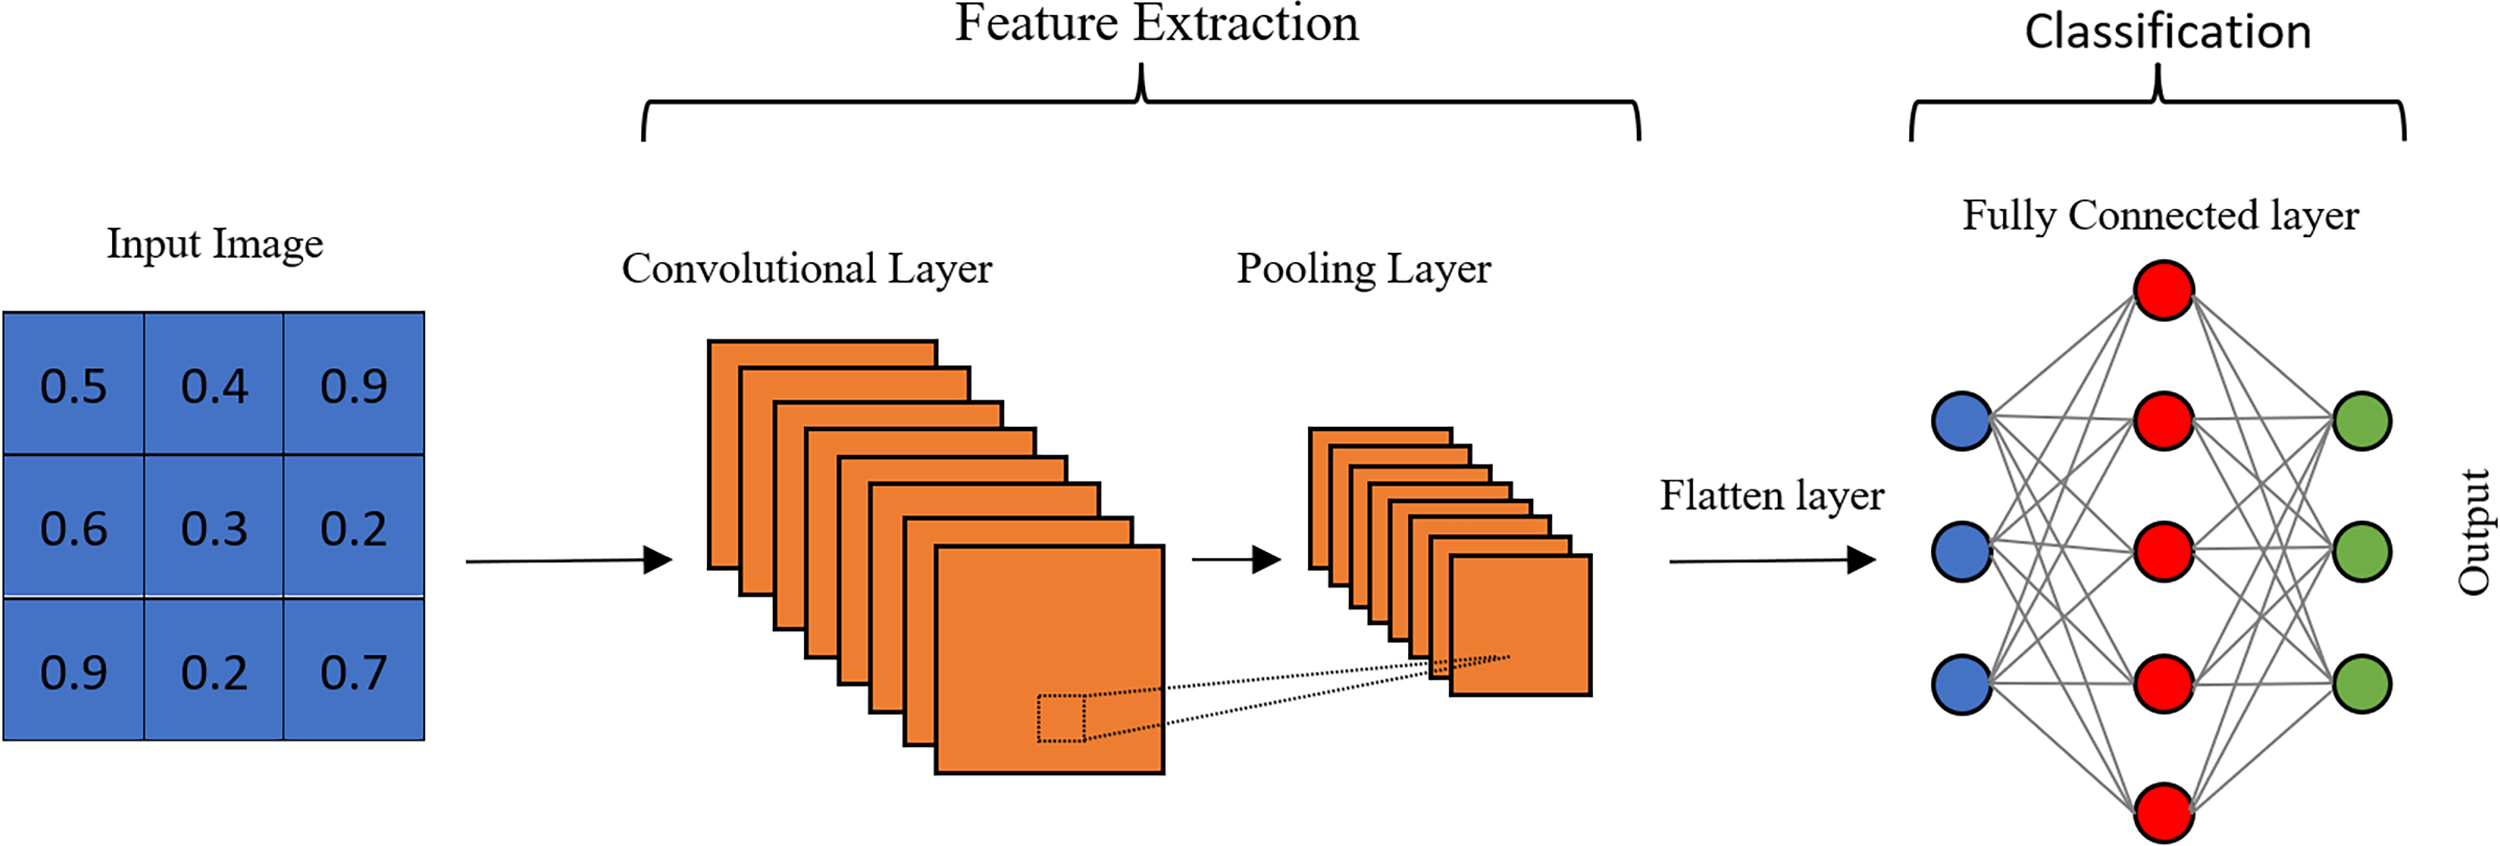
\includegraphics[width=10cm]{arc.png}
	\captionsetup{font=small} % Adjust the font size of the caption
	\captionof{figure}{شکل کلی اتصالات لایه‌های پیچشی, حداکثر ادغام و کاملا متصل در معماری شبکه ساخته شده. لایه ‌های پیچشی و حداکثر ادغام وظیفه اس تخراج ویژگی و لایه‌های ماکلا متصل وظیفه دسته‌بندی را به عهده دارند. نورون‌ها با مدل نورونی نشت‌کننده و ادغام آتش در بین تمام لایه‌های اتصال پیاده‌سازی شده‌اند. }
	\label{fig:arc}
\end{minipage}





تابع رو به جلو \LTRfootnote{\lr{Forward function}}:

در مسیر یادگیری رو به جلو، داده‌های ورودی از طریق لایه‌های پیچشی، حداکثر ادغام و کاملا متصل به صورت گام به گام پردازش می شوند. پتانسیل‌های غشایی نورون‌های LIF در طول مراحل زمانی به روز می‌شوند و اگر پتانسیل غشایی یک نورون از آستانه عبور کند، یک اسپایک خروجی ایجاد می‌شود. اسپایک‌های خروجی در چندین مرحله زمانی جمع‌آوری می‌شوند و به صورت دنباله‌ای از تانسورهای اسپایک بازگردانده می‌شوند.

به طور خلاصه، این شبکه عصبی اسپایکی از لایه‌های پیچشی برای استخراج ویژگی‌ها، لایه‌های نورون LIF برای شبیه‌سازی رفتار عصبی، لایه‌های حداکثر ادغام برای کاهش بعد نمونه‌برداری  و لایه‌های کاملاً متصل برای دسته‌بندی تشکیل شده است. 


در نهایت، با استفاده از لایه‌های پیچشی و مدل‌های نورونی اسپایکی، مدل عصبی می‌تواند ویژگی‌های مهم از داده‌های MNIST و CIFAR-10 استخراج کند و افزایش حجم داده با استفاده از تکنیک‌های گفته‌شده نیز می‌تواند بهبود قابل توجهی در یادگیری مدل ایجاد کند و دقت و عملکرد آن را افزایش دهد و همزمان نیز نیاز به داده برچسب‌دار را کاهش دهد.


\section{انتخاب الگوریتم خودنظارتی مناسب}


انتخاب روش SimCLR برای پیاده‌سازی بر روی شبکه عصبی اسپایکی نسبت به روش‌های خودنظارتی دیگر، دلایل متعددی دارد. از جمله مهم‌ترین دلایل این انتخاب، کارایی و اثربخشی روش SimCLR در یادگیری نمایش‌ها و استخراج ویژگی‌های معنادار از داده‌ها است. SimCLR از دو مرحله اصلی تشکیل شده است که شامل تولید نمونه‌های توسعه‌یافته و استفاده از تابع هدف مبتنی بر تفاوت نمونه‌ها می‌شود. این دو مرحله باعث می‌شوند که مدل با افزایش حجم داده‌ها و تلاش برای افزایش شباهت نمونه‌های مشابه و کاهش تفاوت نمونه‌های مختلف، ویژگی‌های با اهمیت و معنادار از داده‌ها استخراج کند.
در شکل \ref{fig:sim} روش کلی پیاده سازی این الگوریتم نشان داده شده است.

\begin{minipage}{\linewidth}
	\centering
	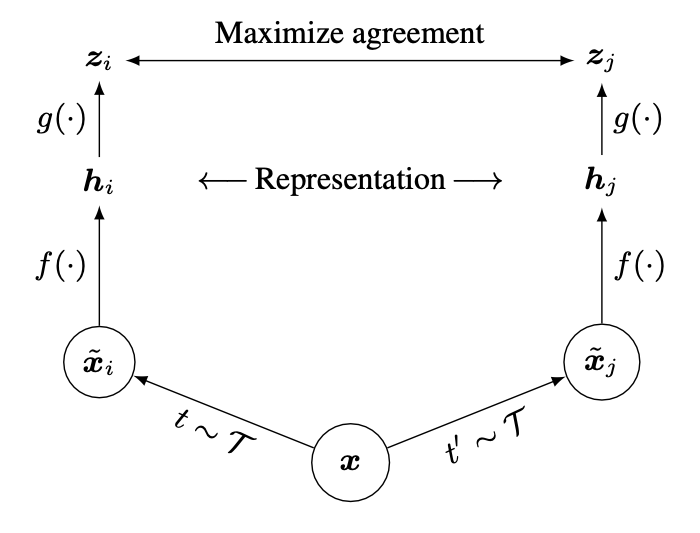
\includegraphics[width=8cm]{simf.png}
	\captionsetup{font=small} % Adjust the font size of the caption
	\captionof{figure}{الگوریتم simclr با کمینه کردن فاصله میان نمونه‌های افزوده شده از یک داده در فضای نمونه, نمایش‌های مناسب از داده بدون برچسب‌را تولید می‌کند.}
	\label{fig:sim}
\end{minipage}


به علاوه، SimCLR به عنوان یکی از روش‌های معتبر یادگیری خودنظارتی، به‌طور گسترده‌ای مورد آزمایش و ارزیابی قرار گرفته است و نتایج بسیار خوبی در استخراج ویژگی‌ها از داده‌ها و بهبود کارایی مدل‌های عصبی حاصل کرده است. این روش می‌تواند بر روی مجموعه‌های داده‌های کوچکتر نیز به‌کار گرفته شود و نیاز به برچسب‌گذاری داده‌ها ندارد .

با توجه به مزیت‌ها و نتایج امتحان‌شده روش SimCLR در حوزه‌های دیگر یادگیری خودنظارتی، انتخاب این روش برای استفاده در شبکه عصبی اسپایکی می‌تواند به عنوان یک انتخاب مناسب و ارزشمند محسوب شود که می‌تواند به بهبود کارایی و عملکرد کلی مدل بسیار کمک کند.







\section{انتخاب تابع هزینه}

در پیاده سازی الگوریتم simclr از تابع هزینه آنتروپی متقاطع با مقیاس دمایی نرمال شده استفاده می شود:


\begin{equation}
	\mathcal{L}_{\text{NTXent}} = -\frac{1}{N} \sum_{i=1}^{N} \log \frac{\exp(\text{sim}(z_i, z_{\text{pos}}) / \tau)}{\sum_{j=1}^{2N} \exp(\text{sim}(z_i, z_j) / \tau)}
\end{equation}

برای پیاده سازی این تابع هزینه با توجه به ساختار نمایش‌های ساخته شده توسط شبکه از کتابخانه pytorch metric learning استفاده کرده ایم. به این صورت که تابع دو نمونه افزوده شده از داده اصلی را به عنوان ورودی می‌گیرد و مقدار شباهت کسینوسی آن را محاسبه کرده و تقسیم بر مجموع همین مقدار برای تمام جفت‌های مثبت می‌کند و در نهایت لگاریتم این مقدار را ذخیره می‌کند.



\section{انتخاب بهینه‌ساز}

بهینه‌ساز یک عنصر کلیدی در فرآیند یادگیری ماشین و شبکه‌های عصبی است. به‌طور کلی، بهینه‌سازها ابزارهایی هستند که در فرآیند تغییر پارامترهای مدل با هدف کمینه کردن تابع هزینه یا خطا به‌کار می‌روند. این پارامترها به‌طور معمول وزن‌ها و بایاس‌های موجود در شبکه‌های عصبی و دیگر پارامترهای مدل یادگیری ماشین را شامل می‌شوند.

هدف اصلی بهینه‌سازها این است که پارامترها را به گونه‌ای تغییر دهند که تابع هزینه کمینه شود. این کار معمولاً با محاسبه گرادیان تابع هزینه نسبت به پارامترها آغاز می‌شود. گرادیان نشان دهنده جهت و شیب تابع در نقاط مختلف است و اطلاعاتی درباره روش تغییرات پارامترها را ارائه می‌دهد.

نوع بهینه‌سازی مورد استفاده می‌تواند تأثیر زیادی بر سرعت و کیفیت یادگیری داشته باشد. بهینه‌سازها ممکن است معیارهای مختلفی را در نظر بگیرند تا در جلوگیری از بیش‌برازش  \LTRfootnote{\lr{Overfitting}}مدل کمک کنند.

استفاده از بهینه‌ساز مناسب می‌تواند به تسریع فرآیند یادگیری، افزایش دقت مدل و جلوگیری از مشکلات مانند بیش‌برازش کمک کند. انتخاب بهینه‌ساز باید با توجه به مساله موردنظر، نوع داده‌ها و معماری مدل انجام شود.

بهینه‌ساز Adam یک روش پیشرفته و موثر در فرآیند یادگیری ماشین و شبکه‌های عصبی است. 
یکی از ویژگی‌های منحصر به فرد Adam، استفاده از نرخ یادگیری انطباقی است. این به معنای تنظیم خودکار نرخ یادگیری بر اساس ویژگی‌های داده‌ها و مساله است. این ویژگی باعث می‌شود Adam به طور خودکار با تغییرات متغیری در داده‌ها، به سرعت به نقاط بهینه همگرا شود.
Adam به طور معمول به سرعت به نقاط بهینه همگرا می‌شود و در مواجهه با داده‌های نویزی نیز خوب عمل می‌کند. از این رو، این بهینه‌ساز به‌طور گسترده در زمینه‌های مختلف یادگیری ماشین و شبکه‌های عصبی مورد استفاده قرار می‌گیرد.

در این پروژه برای پیاده سازی شبکه عصبی اسپایکی با روش یادگیری خودنظارتی از بهینه ساز Adam استفاده شده است. و با استفاده از کتابخانه pytorch پیاده سازی شده است.
\citep{kingma2014adam}

\section{الگوریتم نزدیک ترین همسایه(KNN) }

با توجه به اینکه به وسیله روش یادگیری خودنظارتی شبکه می‌آموزد نمایش هایی از داده اصلی تولید کند برای بررسی اینکه این نمایش های تولید شده چه میزان قابل اعتماد هستند و شبکه تا چه حد آموخته که نمایش مناسبی از داده تولید کند, الگوریتم نزدیک ترین همسایه را برای نمایش‌های تولید شده توسط شبکه پیاده سازی کرده و مشاهده می‌کنیم برای نمونه‌های تصادفی از نمایش‌های تولید شده از داده اصلی نزدیک ترین همسایه‌ها تا چه حد مشابه نمایش‌های تولید شده از داده اصلی هستند. معمولا در الگوریتم نزدیک ترین همسایه با توجه به اکثریت همسایه‌های نمونه که در واقع کمترین معیار فاصله از داده را در فضای نمونه دارند, خود داده اصلی در گروه اکثریت همسایه‌ها با همان برچسب قرار می‌گیرد اما در این پروژه استفاده از الگوریتم نزدیک ترین همسایه برای آزمایش نمایش‌های تولید شده توسط شبکه با الگوریتم یادگیری خودنظارتی است و نتایج آن صرفا برای این هدف مشاهده می‌شوند. در شکل  \ref{fig:knnn}عملکرد کلی این الگوریتم برای یافتن نزدیک ترین همسایه نشان داده شده است.
\citep{guo2003knn}


\begin{minipage}{\linewidth}
	\centering
	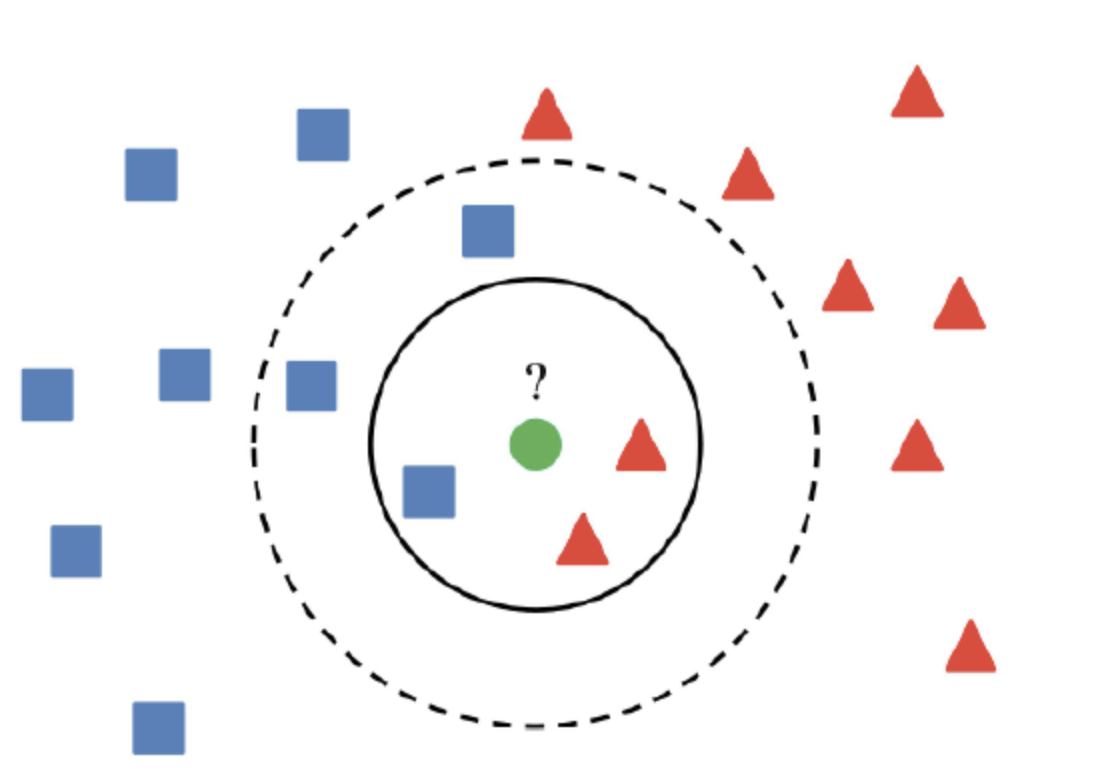
\includegraphics[width=8cm]{knn.png}
	\captionsetup{font=small} % Adjust the font size of the caption
	\captionsetup{font=small} % Adjust the font size of the caption
	\captionof{figure}{الگوریتم نزدیک ترین همسایه}
	\label{fig:knnn}
\end{minipage}


الگوریتم نزدیک‌ترین همسایه (KNN) یکی از الگوریتم‌های یادگیری ماشینی بدون نظارت است که برای دسته‌بندی و پیش‌بینی داده‌ها به کار می‌رود. اصول عمل این الگوریتم بسیار ساده است و بر مفهوم نزدیکی داده‌ها در فضای ویژگی‌ها بنا شده است.

راهکار الگوریتم KNN در پیدا کردن همسایه‌های نزدیک:

فرض کنید ما  مجموعه‌ای از داده‌ها را داریم و می‌خواهیم برای تعدادی نمونه تصادفی که به ما داده می‌شود، نزدیک‌ترین همسایه‌های آن را پیدا کنیم. راهکار الگوریتم KNN به این صورت است:

1. انتخاب تعداد همسایه (K):

ابتدا باید تعداد همسایه‌هایی که می‌خواهیم پیدا کنیم را انتخاب کنیم. این تعداد به عنوان K شناخته می‌شود.

2. محاسبه فواصل:

 برای هر داده ما باید فاصله‌ی آن با تمام داده‌های موجود در مجموعه‌داده را محاسبه کنیم. این فواصل معمولاً با استفاده از معیارهای مختلفی مانند فاصله اقلیدسی یا فاصله کسینوسی محاسبه می‌شوند.

3. انتخاب همسایه‌ها:

سپس تعداد همسایه‌ای که کمترین فواصل را با داده جدید دارند به عنوان همسایه‌های نزدیک انتخاب می‌شوند.
  و در نهایت نتیجه الگوریتم را بر روی نمایش های تولید شده توسط شبکه مشاهده و بررسی می‌کنیم.





\section{دسته‌بندی کننده}



در زمینه یادگیری خودنظارتی، وجود دسته‌بندی کننده \LTRfootnote{\lr{Classifier head}}یک جزء مهم است که برای ارزیابی کیفیت نمایش‌های آموخته‌شده استفاده می‌شود. این یک لایه شبکه عصبی اضافی است که به ویژگی‌های آموخته شده استخراج شده از شبکه  اصلی متصل است. هدف اصلی دسته‌بندی‌کننده، تبدیل نمایش‌های تولیده شده توسط شبکه به برچسب‌های کلاس یا سایر پیش‌بینی‌های مرتبط است که می‌تواند برای وظایف نظارت‌شده استفاده شود.

 دسته‌بندی کننده با استفاده از وظیفه خود نظارتی آموزش داده می شود. این به این معنی است که در طول مرحله آموزش خود‌‌نظارتی، سر دسته‌بندی کننده برای پیش‌بینی برخی ویژگی‌های خاص داده‌های ورودی که به روشی خاص تبدیل یا تقویت شده‌اند، آموزش داده می‌شود. این ویژگی می تواند چرخش، رنگ آمیزی و غیره باشد، بسته به روش خود نظارتی انتخاب شده اند. 
 ابتدا شبکه عصبی پیاده‌سازی شده نمایش‌ها را از داده تقویت شده تولید می‌کند و می آموزد فاصله نمایش های داده‌های یکسان و در یک دسته را بدون برچسب طی فرایند یادگیری خودنظارتی کمینه کند سپس از شبکه آموزش دیده برای به کار گیری در وظایفی مانند دسته بندی نظارت شده استفاده می‌شود. در این مرحله یک دسته بندی کننده که در این پروژه از یک لایه کاملا متصل استفاده می‌شود  بعد نمایش خروجی شبکه را به تعداد دسته‌های نهایی مورد نظر کاهش می‌دهد و از بردار خروجی برای وظایف نظارت‌شده استفاده ‌می‌کند.

به طور خلاصه،  دسته‌بندی کننده در یادگیری خود نظارتی به عنوان پلی بین وظیفه خود نظارت شده و وظایف نظارت‌شده  عمل می کند و به شبکه اجازه می دهد تا نمایش های معنی دار را از داده‌های بدون برچسب یاد بگیرد و سپس این نمایش‌ها را برای کارهای خاص تنظیم یا تطبیق دهد.

در این پروژه ابتدا شبکه با داده بدون برچسب با روش یادگیری خودنظارتی نمایش‌هایی از داده تولید می‌کند و در ادامه شبکه به علاوه  دسته‌بندی کننده با داده با حجم کم برچسب‌دار طی یک فرآیند یادگیری نظارت شده یک عملیات دسته بندی را انجام می‌دهد به این صورت که یک بار شبکه اصلی به عنوان یک ستون  \LTRfootnote{\lr{Backbone}}به  دسته‌بندی کننده متصل می‌شود و با نرخ یادگیری پایین بر روی داده برچسب‌دار با حجم کم آموزش ‌می‌بیند. و یک بار نیز وزن‌های شبکه آموزش دیده شده را ثابت نگه داشته و تنها  دسته‌بندی کننده آموزش می‌بیند و نتایج را مشاهده کرده و با یادگیری از ابتدا نظارت شده مقایسه می‌کنیم.

امید است فرایند یادگیری خودنظارتی در افزایش دقت شبکه در عملیات نهایی دسته بندی با داده برچسب دار با حجم کم موثر واقع شود. در نتیجه در انتهای فرآیند یادگیری شبکه , یک بار نیز همان شبکه را با حجم داده کم و از ابتدا نظارت شده آموزش می‌دهیم تا نتیجه هر دو روش را با هم مقایسه کرده و میزان تاثیر فرایند خودنظارتی را بررسی کنیم.

در شکل \ref{fig:class} یک نمونه از معماری شبکه در یادگیری خودنظارتی نمایش داده شده است که ابتدا یک افزایش داده پیاده‌سازی شده و سپس یک شبکه عصبی اسپایکی با لایه‌های پیچشی و حداکثر ادغام وظیفه تولید نمایش‌های داده را به عهده دارد و در نهایت نیز لایه کاملا متصل دسته‌بندی را روی نمایش‌های تولید شده اعمال کرده و تابع هزینه بر روی آن محاسبه می‌شود.




\begin{minipage}{\linewidth}
	\centering
	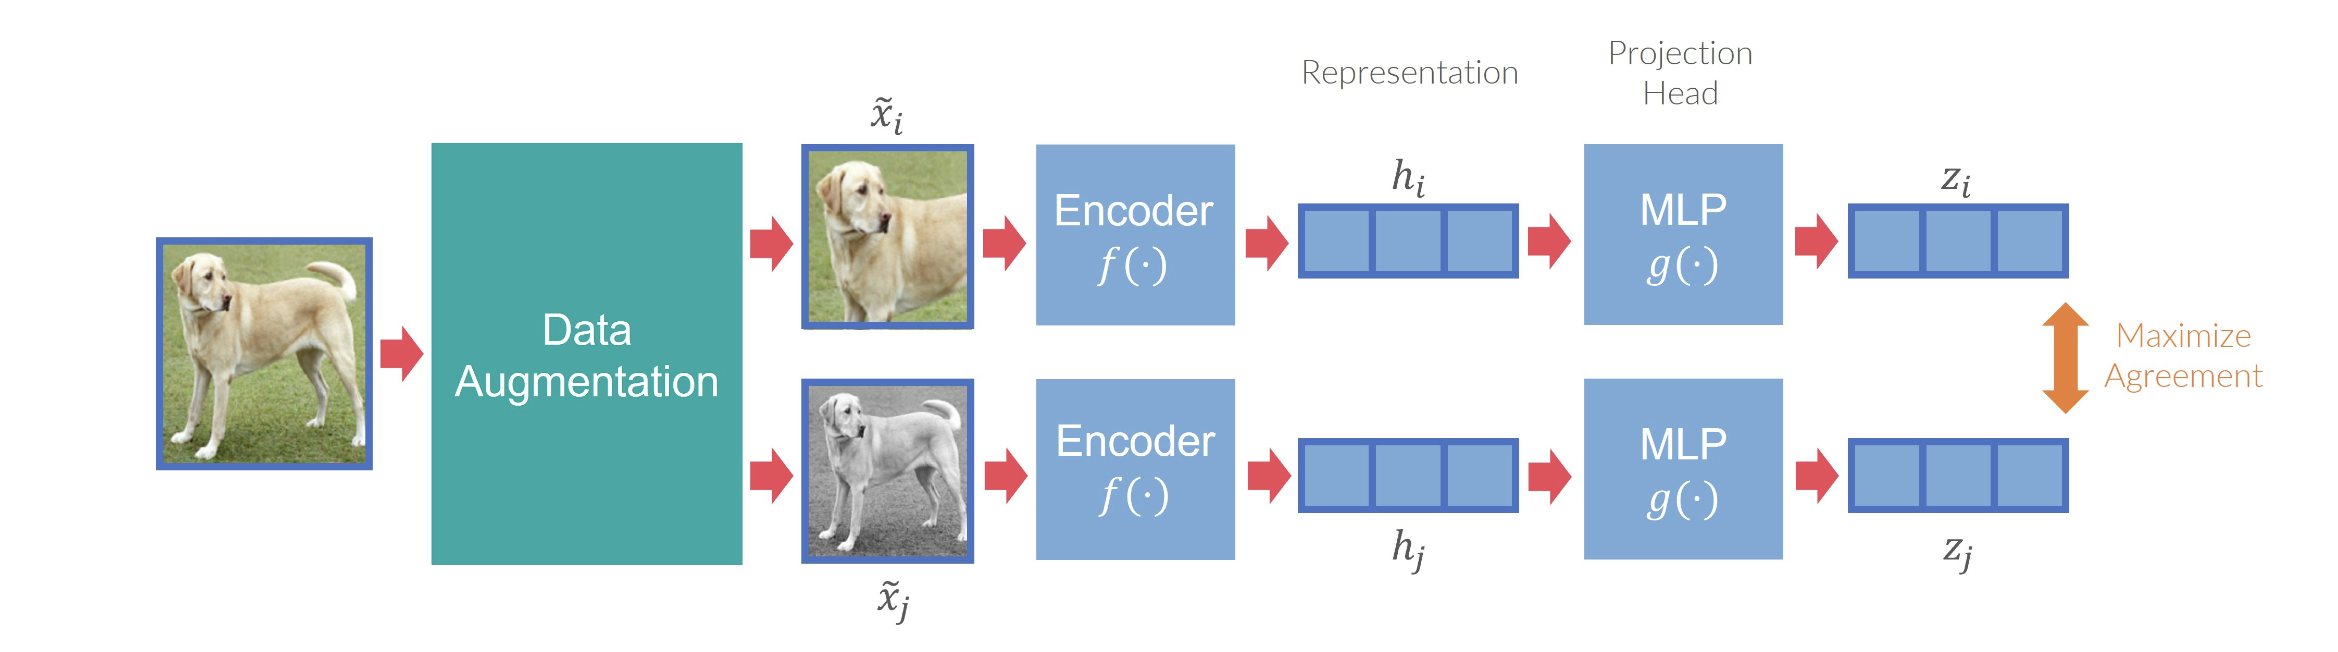
\includegraphics[width=12cm]{class.png}
	%\captionof{figure}{انتقال یادگیری در مقایسه در فرایند یادگیری خودنظارتی}
	\label{fig:class}
\end{minipage}

با توجه به توضیحات داده شده برای پیاده سازی و روش شناسی حل مساله در فصل بعد نتایج پیاده سازی را مشاهده و بررسی می‌کنیم.




	\clearpage
\phantomsection
%\addcontentsline{toc}{chapter}{مقدمات}
\chapter{پیاده سازی و نتایج}
\markboth{پیاده سازی و نتایج}{عنوان فصل}

در این بخش ابتدا پیاده‌سازی مدل نورونی را انجام داده سپس اول از نورون ساخته‌شده در یک شبکه عصبی پیشرو استفاده می‌کنیم و در مرحله بعد معماری شبکه عصبی اسپایکی پیچشی را با مدل نورونی نشت کننده و ادغام آتش پیاده سازی کرده و در نهایت الگوریتم خودنظارتی را به ساختار شبکه اضافه می‌کنیم و نتایج را برای داده های MNIST و CIFAR10 مشاهده و بررسی خواهیم کرد.


\section{پیاده سازی مدل نورونی}

 در ابتدا مدل نورونی را با توجه به آنچه در فصل یک توضیح داده شد پیاده‌سازی کرده و تغییرات پتانسیل و فرآیند تولید اسپایک را بررسی می‌کنیم. همانطور که گفته شد بعد خروجی مدل نورونی برابر است با  :
 
\[
\left[ \text{time step} \times \text{batch size} \times \text{feature dimension} \right]
\]

  و با توجه به اینکه بعد زمان در تانسور خروجی وجود دارد و داده به عنوان جریان ثابت به شبکه در طول گام های زمانی داده شده است, برای بررسی روند تولید اسپایک, تغییرات پتانسیل هر نورون را در طول گام‌های زمانی جمع بسته و بررسی می‌کنیم آیا پتانسیل از آستانه عبور کرده یا خیر.
در شکل  \ref{fig:liff} یک نمونه از جریان ثابت ورودی و یک نمونه از خروجی نورون که شامل تغییرات پتانسیل و گسیل اسپایک می‌شود نشان داده‌شده است.

\begin{minipage}{\linewidth}
	\centering
	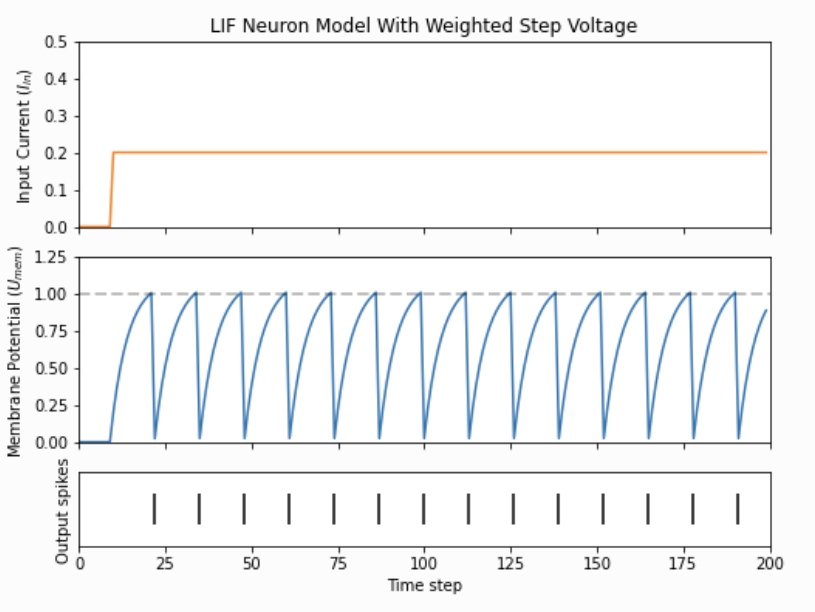
\includegraphics[width=8cm]{lif.png}
	\captionsetup{font=small} % Adjust the font size of the caption
	\captionof{figure}{پیاده‌سازی مدل نورونی نشت‌کننده و ادغام آتش ونمایش تولید اسپایک در صورت عبور پتانسیل از آستانه}
	\label{fig:liff}
\end{minipage}







\section{پیاده سازی یادگیری خودنظارتی روی شبکه عصبی اسپایکی}
برای ساخت اتصالات بین نورون ها از اتصالات پیچشی و کاملا متصل استفاده می‌کنیم به این صورت که لایه‌های اسپایکی خروجی‌های اسپایک و تغییرات پتانسیل غشا را تولید می‌کنند و لایه‌های پیچشی و کاملا متصل نوع اتصال نورون ها را مشخص می‌کنند.
% ساختار شبکه به صورت زیر است :
%
%1. لایه پیچشی ۱ (conv1):
%
%این لایه یک لایه پیچشی دوبعدی است که ورودی‌های ۳ کانال را به ۳۲ کانال تبدیل می‌کند. این لایه ورودی‌ها را با یک فیلتر به اندازه ۲در۲ کوچکتر می‌کند.
%
%2. لایه اسپایکی ۱ (lif1):
%این لایه یک لایه فعال‌سازی است که برای نورون‌های اسپایکی از آن استفاده می‌شود و بردار اسپایک و تغییرات پتانسیل را به عنوان خروجی می‌دهد.
%
%3. لایه پیچشی ۲ (conv2):
%این لایه نتایج خروجی از لایه اسپایکی قبلی را با یک فیلتر دیگر به اندازه ۲در۲ کوچکتر می‌کند و به ۶۴  کانال تبدیل می‌کند.
%
%4. لایه اسپایکی ۲ (lif2):
% این لایه نیز برای فعال‌سازی نورون‌های اسپایکی استفاده می‌شود و با پارامتر بتا تنظیم می‌شود.
%
%5. لایه پیچشی ۳ (conv3):
%این لایه به عنوان یک لایه پیچشی جدید اضافه شده است که ورودی‌ها را با یک فیلتر دیگر به ۱۲۸ کانال تبدیل می‌کند.
%
%6. لایه اسپایکی ۳ (lif3):
%همانند لایه‌های  قبلی، این لایه نیز برای فعال‌سازی نورون‌های اسپایکی اضافه شده و با تنظیم پارامتر بتا کار می‌کند.
%
%7. لایه پیچشی ۴ (conv4):
%این لایه نتایج خروجی از لایه پیچشی جدید قبلی را با یک فیلتر دیگر به اندازه ۲در۲ کوچکتر می‌کند و به ۲۵۶  کانال تبدیل می‌کند.
%
%8. لایه اسپایکی ۴ (lif4):
%همانند لایه‌های اسپایکی  قبلی، این لایه نیز برای فعال‌سازی نورون‌های اسپایکی اضافه شده است.
%
%9. لایه خطی ۱ (fc1):
%این لایه اتصالات خطی دارد و ورودی‌ها را به یک بردار ۵۱۲ بعدی تبدیل می‌کند. 
%
%10. لایه اسپایکی ۵ (lif5):
% این لایه نیز برای فعال‌سازی نورون‌های اسپایکی اضافه شده است.
%
%11. لایه خطی ۲ (fc2):
%این لایه خطی یک لایه جدید با ورودی‌های ۵۱۲ بعدی را به یک بردار ۳۲ بعدی تبدیل می‌کند.
%
%12. لایه اسپایکی ۶ (lif6):
%این لایه نیز برای فعال‌سازی نورون‌های اسپایکی اضافه شده و با تنظیم پارامتر بتا کار می‌کند. این لایه به لایه خطی ۲ اعمال می‌شود.

برای پیاده سازی بخش خودنظارتی هر بار دو نمونه از داده افزوده‌شده را در دسته‌های با اندازه‌های مختلف به شبکه داده و تابع هزینه را روی خروجی شبکه که در طول زمان جمع بسته شده اعمال می‌کنیم و فرآیند آموزش را طی می‌کنیم تا شبکه بیاموزد نمایش‌های مناسب از داده را تولید کند. نمودار تغییر تابع هزینه را در طول زمان مشاهده می‌کنیم و به این معناست که شبکه در حال آموختن است. با توجه به اینکه در این مرحله فرایند آموزش با داده بدون برچسب اتفاق می‌افتد تنها تغییر تابع هزینه بر روی مجموعه داده آموزشی  در شکل‌های  \ref{fig:loss1} و  \ref{fig:loss2}  قابل مشاهده است.


% \begin{minipage}{\linewidth}
% 	\raggedleft
% 	\includegraphics[width=8cm]{mnistloss.png}
% 	\captionof{figure}{نمودار تابع هزینه شبکه برای مجموعه داده  mnist}
% 	\label{fig:kknnn}
% \end{minipage}
% 
 
\begin{minipage}{0.49\linewidth}
	\centering
	\includegraphics[width=\linewidth]{mnistloss.png}
	\captionsetup{font=small} % Adjust the font size of the caption
	\captionof{figure}{نمودار تابع هزینه شبکه برای مجموعه داده  mnistدر فرایند یادگیری خودنظارتی}
	\label{fig:loss1}
\end{minipage}
%\hspace{0.01\textwidth}
\begin{minipage}{0.49\linewidth}
	\centering
	\includegraphics[width=\linewidth]{cifarloss.png}
	\captionsetup{font=small} % Adjust the font size of the caption
	\captionof{figure}{نمودار تابع هزینه شبکه برای مجموعه داده  cifar فرایند یادگیری خودنظارتی}
	\label{fig:loss2}

\end{minipage}




سپس برای آزمایش نمایش‌های تولید شده و آزمودن عملکرد شبکه یک بار نمایش‌ها را به عنوان ورودی به الگوریتم نزدیک‌ترین همسایه می‌دهیم و بررسی می‌کنیم و یک بار نیز  دسته‌بند را به عنوان لایه آخر به شبکه اضافه می‌کنیم و بعد نمایش خروجی را به اندازه تعداد دسته داده که در این پروژه برای هر دو مجموعه داده MNIST , CIFAR10 تعداد ۱۰ است کاهش می‌دهیم و طی یک فرایند آموزش نظارت شده دقت شبکه را می‌سنجیم.


\section{پیاده سازی الگوریتم نزدیک ترین همسایه }
از کتابخانه sklearn برای پیاده کردن الگوریتم استفاده کرده و بر روی دو مجموعه داده آزمایش کرده ایم به این صورت که چند نمایش خروجی از شبکه را به صورت تصادفی انتخاب کرده و ده همسایه نزدیک به آن را مشاهده کرده ایم . با توجه به شکل  \ref{fig:kknnn} مشاهده می‌شود که الگوریتم نزدیک ترین همسایه نمایش‌های مشابه را برای نمونه‌های تصادفی از خروجی شبکه به درستی تشخیص داده است.


\begin{minipage}{\linewidth}
	\centering
	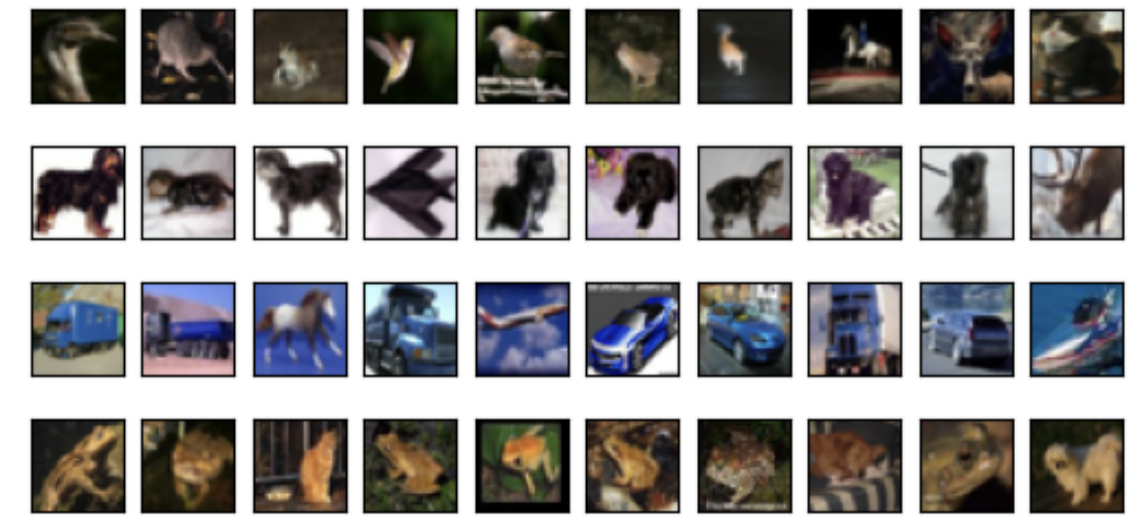
\includegraphics[width=8cm]{knnn.png}
	\captionsetup{font=small} % Adjust the font size of the caption
	\captionof{figure}{نمونه خروجی الگوریتم نزدیک ترین همسایه بر روی نمایش های تولید شده توسط شبکه عصبی اسپایکی در طول یادگیری خودنظارتی}
	\label{fig:kknnn}
\end{minipage}



\section{  پیاده سازی دسته بندی کننده و نتایج }

برای اضافه کردن دسته‌بندی‌کننده از یک لایه خطی کاملا متصل استفاده می‌کنیم که بعد تانسور خروجی را به تعداد دسته‌ها در داده کاهش می‌دهد و با جمع بستن خروجی در طول زمان هر درایه‌ای در تانسور خروجی اسپایک که بیشترین فعالیت را داشته باشد به عنوان برچسب مربوط به آن داده در نظر گرفته می‌شود. لازم به ذکر است چون یکی از اهداف مهم یادگیری خودنظارتی کم کردن نیاز به داده برچسب دار است در این مرحله از فرآیند آموزش شبکه با حدود ۲۰٪ از حجم داده اصلی آموزش می‌بیند. در صورتی که ۸۰٪ از داده برای آموزش خودنظارتی شبکه استفاده شده است.
در شکل‌های \ref{fig:closs1} و  \ref{fig:closs2}  تغییر تابع هزینه در طول فرآیند یادگیری نظارت شده را مشاهده می‌کنیم.


\begin{minipage}{0.49\linewidth}
	\centering
	\includegraphics[width=\linewidth]{cmnist.png}
	\captionsetup{font=small} % Adjust the font size of the caption
	\captionof{figure}{نمودار تابع هزینه شبکه برای مجموعه داده  MNIST فرایند یادگیری نظارت شده با ۲۰٪ حجم داده}
	\label{fig:closs1}
\end{minipage}
%\hspace{0.01\textwidth}
\begin{minipage}{0.49\linewidth}
	\centering
	\includegraphics[width=\linewidth]{ccifar.png}
	\captionsetup{font=small} % Adjust the font size of the caption
	\captionof{figure}{نمودار تابع هزینه شبکه برای مجموعه داده  CIFAR فرایند یادگیری نظارت شده با ۲۰٪ حجم داده}
	\label{fig:closs2}
	
\end{minipage}

پارامترهایی همچون اندازه دسته , انتخاب روش افزودن داده و تعداد گام زمانی در عملکرد نهایی شبکه تاثیرگذارند. در جدول‌های زیر آزمایش‌های انجام شده برای مشاهده تاثیر هر یک از پارامتر‌ها نشان داده شده است. 





\begin{table}[h!]
	%\caption{Multi-column Table}
	\centering
	\begin{tabular}{|c |c c| rrrrrrr}
			\hline
		اندازه دسته & MNIST & CIFAR10    \\ 
		\hline
		64   & 45.77    &76.52     \\
		%\hline
		128    & 87.79     & 28.55      \\
		%\hline
		256   & 13.82     & 79.58         \\
		\hline
		
	\end{tabular}
	\captionsetup{font=small} % Adjust the font size of the caption
	\caption{ درصد دقت عملکرد شبکه با توجه به اندازه دسته‌های مختلف}
\end{table}



\begin{table}[h!]
	%\caption{Multi-column Table}
	\centering
	\begin{tabular}{|c |c c| rrrrrrr}
		\hline
		گام زمانی & MNIST & CIFAR10    \\ 
		\hline
		10   & 21.78     &63.53    \\
		%\hline
		20    & 54.81     & 84.57     \\
		%\hline
		30   & 34.82    & 15.58         \\
		\hline
		
	\end{tabular}
	\captionsetup{font=small} % Adjust the font size of the caption
	\caption{درصد دقت عملکرد شبکه با توجه به گام های زمانی مختلف}
\end{table}


\begin{table}[h!]
	%\caption{Multi-column Table}
	\centering
	\begin{tabular}{|c |c c| rrrrrrr}
		\hline
		روش افزودن داده & CIFAR10& MNIST     \\ 
		\hline
		برش - چرخش   & 21.55      &43.81     \\
		%\hline
		برش - نویز گاوسی    & 12.56     & 06.82      \\
		%\hline
		چرخش - نویز گاوسی   & 54.58     & 23.82          \\
		\hline
		
	\end{tabular}
	\captionsetup{font=small} % Adjust the font size of the caption
	\caption{درصد دقت عملکرد شبکه با توجه به روش‌های مختلف افزودن داده}
\end{table}






از طرفی با توجه به اینکه هدف اصلی اعمال یادگیری خودنظارتی بر روی شبکه, بی‌نیاز کردن یادگیری از داده برچسب‌دار است انتظار می‌رود پس از اعمال این فرآیند, شبکه از فرآیند یادگیری نظارت شده روی داده برچسب دار با حجم کم دقت بهتری داشته باشد.در نتیجه یک بار نیز شبکه با همان معماری را به صورت نظارت‌شده بر روی داده با حجم کم(۲۰٪ از حجم کل داده) آموزش می‌دهیم و نتایج را مقایسه می‌کنیم . 
پس از آزمایش‌های انجام شده نتیجه گرفتیم که شبکه عصبی اسپایکی با فرآیند یادگیری خودنظارتی عملکرد بهتری از آموزش نظارت شده برای داده‌های برچسب‌دار با حجم کم دارد.

در نمودارهای  \ref{fig:acc1} و  \ref{fig:acc2}دقت هریک از روش‌های خودنظارتی و نظارت شده بر روی مجموعه داده‌های MNIST , CIFAR10 نشان داده شده است.


\begin{minipage}{0.49\linewidth}
	\centering
	\includegraphics[width=\linewidth]{macc.png}
	\captionsetup{font=small} % Adjust the font size of the caption
	\captionof{figure}{مقایسه دقت عملکرد روش‌های یادگیری خودنظارتی و نظارت‌شده بر روی مجموعه داده MNIST}
	\label{fig:acc1}
\end{minipage}
%\hspace{0.01\textwidth}
\begin{minipage}{0.49\linewidth}
	\centering
	\includegraphics[width=\linewidth]{cacc.png}
	\captionsetup{font=small} % Adjust the font size of the caption
	\captionof{figure}{مقایسه دقت عملکرد روش‌های یادگیری خودنظارتی و نظارت شده بر روی مجموعه داده CIFAR10}
	\label{fig:acc2}
\end{minipage}

همانطور که مشاهده می‌شود پیاده سازی روش یادگیری خودنظارتی موجب افزایش دقت عملکرد شبکه شده‌است. و همچنان نیاز به داده برچسب‌دار را بسیار کاهش داده و با توجه به اینکه روش یادگیری خودنظارتی بر روی شبکه‌های اسپایکی اعمال شده به علت ساختار این شبکه‌ها, نیاز به مصرف انرژی برای یادگیری نیز کاهش پیدا کرده و فرایند آموزش بهینه ‌تر انجام شده است.




\section{چشم انداز پژوهشی}

 با توجه به اینکه پیاده‌سازی روش‌های یادگیری خودنظارتی بر روی شبکه‌های عصبی اسپایکی یک حوزه پژوهشی نوآورانه و جذاب محسوب می‌شود، امکانات بی‌نظیری را برای بهبود کاربردها و پیشرفت در علم و فناوری فراهم می‌کند. این پیشرفت در ارتقاء روش‌های یادگیری و استفاده از داده‌های پیچیده‌تر، می‌تواند اثرات مثبتی بر تحقیقات مختلف داشته باشد.
 با توجه به چالش کمبود داده برچسب‌دار و هزینه و زمان‌بر بودن فرآیند تولید برچسب برای داده, این چالش ممکن است مانع از استفاده کامل از روش‌های یادگیری تقویتی و عمقی شود. 
 
 از طرفی با توجه به ماهیت بیولوژیکی شبکه‌های عصبی اسپایکی و بهینه بودن آن‌ها در مصرف انرژی زمان نسبت به شبکه‌های عصبی مصنوعی, استفاده از این شبکه‌ها منجر به پیشرفت‌هایی در حوزه‌های مختلف یادگیری و علوم اعصاب خواهد شد.
 با پیاده‌سازی روش‌ یادگیری خودنظارتی بر روی شبکه‌های عصبی اسپایکی، می‌توان به صورت تخمینی و بدون نیاز به داده‌های برچسب‌دار، توانایی‌های شبکه‌ها در تشخیص الگوها و اطلاعات مهم را بهره‌برداری کرد. این روش، باعث تولید ابزاری مؤثر در ایجاد نمایندگان با کیفیت از داده‌ها می‌شود که می‌تواند در کاربردهای متعددی در زمینه‌های مختلف مانند تشخیص بیماری‌ها، پیش‌بینی تغییرات و... مفید واقع شود.
 امید است این ابزار محاسباتی در حوزه‌های مختلف یادگیری مفید واقع شود و بتوان به این وسیله در مسائل مختلف یادگیری ماشین و پردازش داده تصویری موجب پیشرفت شد.
 
 در ادامه روند این پژوهش بنا داریم با پیچیده‌تر کردن شبکه و بررسی پارامتر‌ها عملکرد شبکه را بهبود بخشیم و با افزایش دقت شبکه یک ابزار قوی و قابل اعتماد محاسباتی تولید کنیم که نه تنها نیاز به داده‌برچسب‌دار را کاهش دهد بلکه در مصرف انرژی و حافظه نیز بهینه باشد.
 
	
	\backmatter
	{\small
		{\baselineskip=.75cm
			%%%%%%%%%%%%%%%%%%
			\addcontentsline{toc}{chapter}{واژه‌نامه فارسی به انگلیسی}
\thispagestyle{empty}
\chapter*{واژه‌نامه فارسی به انگلیسی}
\markboth{واژه‌نامه فارسی به انگلیسی}{واژه‌نامه فارسی به انگلیسی}

\noindent

% ... Add more entries ...
% Spiking Neural Network related glossary
\englishgloss{Neuron}{نورون}
\englishgloss{Neural Network}{شبکه عصبی}
%\englishgloss{Reinforcement}{تقویت‌شده}
\englishgloss{Machine Learning}{یادگیری ماشینی}
\englishgloss{Information}{اطلاعات}
\englishgloss{Transfer}{انتقال}
\englishgloss{Computer Vision}{بینایی ماشین}
\englishgloss{Image}{تصویر}
\englishgloss{Data}{داده‌ها}
\englishgloss{Data Augmentation}{افزایش داده}
\englishgloss{Classification}{طبقه‌بندی}
\englishgloss{Supervised Learning}{آموزش با نظارت}
\englishgloss{Unsupervised Learning}{آموزش بدون نظارت}
\englishgloss{Semi-Supervised Learning}{آموزش نیمه‌نظارتی}
%\englishgloss{Sequential Actions}{کنش‌های زنجیره‌ای}
\englishgloss{Transfer Learning}{یادگیری انتقالی}
%\englishgloss{Principled Analysis}{تجزیه و تحلیل اصولی}
\englishgloss{Outlier Detection}{تشخیص نمونه‌های خارجی}
\englishgloss{Unsupervised Learning}{یادگیری نظارت‌نشده}
\englishgloss{Similarity}{شباهت}
%\englishgloss{Parallel Actions}{کنش‌های موازی}
\englishgloss{Data Visualization}{تصویرسازی داده‌ها}
\englishgloss{Comparative Methods}{روش‌های مقایسه‌ای}
\englishgloss{Learning Algorithms}{الگوریتم‌های یادگیری}
\englishgloss{Neural Network Models}{مدل‌های شبکه عصبی}
\englishgloss{Self-Supervised Learning}{آموزش خودنظارتی}
\englishgloss{k-Nearest Neighbor Algorithm (k-NN)}{الگوریتم k نزدیک‌ترین همسایه (k-NN)}
\englishgloss{Spiking Neural Network (SNN)}{شبکه عصبی اسپایکی (SNN)}
\englishgloss{Spiking Neuron}{نورون عصبی اسپایکی}
%\englishgloss{Chip Threshold}{آستانه تراشه‌ای}
\englishgloss{Spike-based Information Transmission}{انتقال اطلاعات با پالس‌ها}
\englishgloss{Spike Propagation Delay}{تاخیر انتشار پالس}
\englishgloss{Neural Layer Structure}{ساختار لایه نورونی}
\englishgloss{Input Synapses}{سیناپس‌های ورودی}
\englishgloss{Output Synapses}{سیناپس‌های خروجی}
\englishgloss{Hodgkin-Huxley Model}{مدل هادجکین-هاکسلی}
\englishgloss{Dynamic Equilibrium Point}{نقطه توازن دینامیکی}
\englishgloss{Neuron Training Algorithms}{الگوریتم آموزش نورون‌ها}
\englishgloss{Artificial Neuron}{نورون مصنوعی}
%\englishgloss{Spike-based Information Processing}{استفاده از پالس‌ها برای پردازش اطلاعات}
\englishgloss{Spike-based Neural Network}{شبکه عصبی پالسی}
\englishgloss{Electric Pulse (Spike)}{پالس الکتریکی}
\englishgloss{Membrane Potential}{پتانسیل غشایی}
\englishgloss{Threshold Ceiling}{سقف آستانه}
\englishgloss{Membrane Potential Threshold}{آستانه پتانسیل غشایی}
\englishgloss{Image Resizing}{تغییر اندازه تصویر}
\englishgloss{Image Rotation}{چرخش تصویر}
\englishgloss{Image Cropping}{برش تصویر}
\englishgloss{Adding Noise}{افزودن نویز}
\englishgloss{Image Brightness Adjustment}{تغییر روشنایی تصویر}
%\englishgloss{Image Contrast Adjustment}{تغییر کنتراست تصویر}
\englishgloss{Image Flipping}{انعکاس تصویر}
\englishgloss{Image Perspective Transformation}{تغییر زاویه تصویر}
\englishgloss{Applying Image Effects}{اعمال افکت‌های تصویری}
\englishgloss{Changing Color Channel Order}{تغییر ترتیب کانال‌های رنگی}
\englishgloss{Image Intensity Adjustment}{تغییر شدت تصویر}

			\addcontentsline{toc}{chapter}{واژه‌نامه  انگلیسی به  فارسی}
\thispagestyle{empty}
\chapter*{واژه‌نامه  انگلیسی به  فارسی}
\markboth{واژه‌نامه  انگلیسی به  فارسی}{واژه‌نامه  انگلیسی به  فارسی}
\noindent

\persiangloss{نورون}{neuron}
\persiangloss{تیزه}{spike}
\persiangloss{سیناپس}{synapse}
\persiangloss{یادگیری خودنظارتی}{self-supervised learning}
\persiangloss{بینایی کامپیوتری}{computer vision}
\persiangloss{ماژول}{module}
\persiangloss{پرسپترون}{perceptron}
\persiangloss{نویز}{noise}
\persiangloss{متضاد}{contrastive}
\persiangloss{فضای نمونه}{embedding space}
\persiangloss{فاصله اقلیدسی}{Euclidean Distance}
\persiangloss{شباهت کسینوسی}{Cosine Similarity}
\persiangloss{اطلاعات}{Information}
\persiangloss{انتقال}{Transfer}
\persiangloss{تصویر}{Image}
\persiangloss{داده‌ها}{Data}
\persiangloss{افزایش داده}{Data Augmentation}
\persiangloss{طبقه‌بندی}{Classification}
\persiangloss{آموزش با نظارت}{Supervised Learning}
\persiangloss{آموزش بدون نظارت}{Unsupervised Learning}
\persiangloss{آموزش نیمه‌نظارتی}{Semi-Supervised Learning}
\persiangloss{یادگیری انتقالی}{Transfer Learning}
\persiangloss{تشخیص نمونه‌های خارجی}{Outlier Detection}
\persiangloss{شباهت}{Similarity}
\persiangloss{تصویرسازی داده‌ها}{Data Visualization}
\persiangloss{روش‌های مقایسه‌ای}{Comparative Methods}
\persiangloss{الگوریتم‌های یادگیری}{Learning Algorithms}
\persiangloss{مدل‌های شبکه عصبی}{Neural Network Models}
\persiangloss{شبکه عصبی اسپایکی}{Spiking Neural Network (SNN)}
\persiangloss{نورون عصبی اسپایکی}{Spiking Neuron}
\persiangloss{انتقال اطلاعات با پالس‌ها}{Spike-based Information Transmission}
\persiangloss{تاخیر انتشار پالس}{Spike Propagation Delay}
\persiangloss{ساختار لایه نورونی}{Neural Layer Structure}
\persiangloss{سیناپس‌های ورودی}{Input Synapses}
\persiangloss{سیناپس‌های خروجی}{Output Synapses}
\persiangloss{مدل هادجکین-هاکسلی}{Hodgkin-Huxley Model}
\persiangloss{نقطه توازن دینامیکی}{Dynamic Equilibrium Point}
\persiangloss{الگوریتم آموزش نورون‌ها}{Neuron Training Algorithms}
\persiangloss{نورون مصنوعی}{Artificial Neuron}
\persiangloss{استفاده از پالس‌ها برای پردازش اطلاعات}{Spike-based Information Processing}
\persiangloss{شبکه عصبی پالسی}{Spike-based Neural Network}
\persiangloss{پالس الکتریکی}{Electric Pulse (Spike)}
\persiangloss{پتانسیل غشایی}{Membrane Potential}
\persiangloss{سقف آستانه}{Threshold Ceiling}
\persiangloss{آستانه پتانسیل غشایی}{Membrane Potential Threshold}
\persiangloss{تغییر اندازه تصویر}{Image Resizing}
\persiangloss{چرخش تصویر}{Image Rotation}
\persiangloss{برش تصویر}{Image Cropping}
\persiangloss{افزودن نویز}{Adding Noise}
\persiangloss{تغییر روشنایی تصویر}{Image Brightness Adjustment}
\persiangloss{تغییر کنتراست تصویر}{Image Contrast Adjustment}
\persiangloss{انعکاس تصویر}{Image Flipping}
\persiangloss{تغییر زاویه تصویر}{Image Perspective Transformation}
\persiangloss{اعمال افکت‌های تصویری}{Applying Image Effects}
\persiangloss{تغییر ترتیب کانال‌های رنگی}{Changing Color Channel Order}
\persiangloss{تغییر شدت تصویر}{Image Intensity Adjustment}

			{\baselineskip=.6cm
				\phantomsection
				\addcontentsline{toc}{chapter}{نمایه}
				\printindex}
			\phantomsection
			\addcontentsline{toc}{chapter}{مراجع }
			%\bibliography{ref.bib}{}
			%\bibliographystyle{unsrtnat}
			\bibliographystyle{chicago-fa}%{chicago-fa}
			\begin{flushleft}
				\bibliography{ref}
			\end{flushleft}
			
			%%%%%%%%%%%%%%%
			%ایجاد صفحه‌ای سفید%%%%%%%%%%%%%%%%%%%%%%%%%%%%%%%%%%%
			\cleardoublepage % Ensure the blank page starts on a right-hand page
			
			\newpage
			\thispagestyle{empty}
			\clearpage
			~~~
			%%%%%%%%%%%%%%%%%%%%%%%%%%%%%%%%%%%%
			% در این فایل، عنوان پایان‌نامه، مشخصات خود و چکیده پایان‌نامه را به انگلیسی، وارد کنید.
% توجه داشته باشید که جدول حاوی مشخصات پایان‌نامه/رساله، به طور خودکار، رسم می‌شود.
%%%%%%%%%%%%%%%%%%%%%%%%%%%%%%%%%%%%
\baselineskip=0.6cm
\begin{latin}
\latinuniversity{Shahid Beheshti University}
\latinfaculty{Faculty of Mathematical Sciences}
\latindegree{Master}
%group:
\latinsubject{Department of Data \& Computer Science}
\latinfield{Computer Sciences - Data Mining}
\latintitle{self-supervised learning on spiking neural network}
\firstlatinsupervisor{Dr.Hadi Farahani}
\secondlatinsupervisor{Dr. Saeed Reza Kheradpisheh}
%\firstlatinadvisor{Dr. ZZZ}
%\secondlatinadvisor{Second Advisor}
\latinname{Yeganeh}
\latinsurname{Bahari Asl}
\latinthesisdate{September 2023}
\latinkeywords{Spiking neural networks, self-supervised learning, data classification}
\en-abstract{\noindent 
In this thesis, we examine and introduce spiking neural networks as a new generation of neural networks. Inspired by the structure of the brain, these networks encode and process information through precisely timed spike trains. Unlike the rest of the neural networks, in this type of network, the neurons are resting except when generating spikes, and this property makes the structure of these networks optimal and uses less memory.
In this research, we investigate self-supervised learning methods in spiking neural networks. This method has the ability to use techniques such as data augmentation to perform learning in a redundant network of labeled data.
Finally, the aim of this research is to build an optimal spiking neural network with the capability of self-supervised learning methods to generate representations from the MNIST and CIFAR10 datasets without the need for data labels, and to use these representations for various tasks such as supervised classification. This research tries to finally create more accuracy on the classification methods on the data set by making these representations.
}
\latinvtitle
\end{latin}
			\label{LastPage}
		}
	}
\end{document}













%
%\documentclass[a4paper,11pt,msc]{SBU}
%
%% در این فایل، دستورها و تنظیمات مورد نیاز، آورده شده است.
%-------------------------------------------------------------------------------------------------------------------

\usepackage{stmaryrd}
\usepackage{amssymb,amsmath,amsthm}
\usepackage{mathrsfs}
\usepackage [justification=centering]{caption}
%ایجاد فرورفتگی در اولین پاراگراف هر بخش
\usepackage{indentfirst}
% بسته‌ای برای تنطیم حاشیه‌های بالا، پایین، چپ و راست صفحه
\usepackage[top=30mm, bottom=30mm, left=25mm, right=35mm]{geometry}
% بسته‌‌ای برای ظاهر شدن شکل‌ها و تصاویر متن
\usepackage{graphicx}
%\usepackage{mdframed}
\usepackage{caption}
%\usepackage{subcaption}
\usepackage{rotating}
\usepackage{pdflscape}
%\usepackage{subcaption}
\usepackage{mwe}
\usepackage{subfig}
%\usepackage{subcaption}
\usepackage{graphicx}
%\usepackage{tabu}
\usepackage{multirow}
\usepackage{siunitx}
\usepackage{booktabs}
\usepackage{hhline}
\usepackage{setspace}
%\usepackage{rotating}
%\usepackage{underscore}
\usepackage[usenames,dvipsnames]{color}
\usepackage{bbding}
\usepackage{xecolor}
\usepackage{bbold}

 
\usepackage{rotating}
\setlength{\rotFPtop}{0pt plus 1fil}


%\usepackage{xcolor}
\def\BibTeX{{\rm B\kern-.05em{\sc i\kern-.025em b}\kern-.08em
    T\kern-.1667em\lower.7ex\hbox{E}\kern-.125emX}}

% بسته‌های نوشتن شبه کد و الگوریتم
%\usepackage{algorithm} 
%\usepackage{algorithmic} 
\usepackage[algochapter,linesnumbered,ruled,vlined]{algorithm2e}
% بسته‌ای برای رسم کادر
\usepackage{framed} 
% بسته‌‌ای برای چاپ شدن خودکار تعداد صفحات در صفحه «معرفی پایان‌نامه»
\usepackage{lastpage}
% بسته‌‌ای برای ایجاد دیاگرام‌های مختلف
\usepackage[all]{xy}
\usepackage{tikz}

%\usepackage{zref-perpage}
%\zmakeperpage{footnote}

\usepackage{zref-abspage}
%\zmakeperpage{footnote}

\usepackage{perpage}
%\MakePerPage{footnote}

\usetikzlibrary{topaths}
\tikzset{terminal/.style={
							% The shape:
							rectangle ,minimum size =6mm,rounded corners=4mm,
							% The rest
							%very thick,draw=black!50,
							top color=green!10,bottom color=green!40,
							font=\ttfamily}}
	\renewcommand{\baselinestretch}{2}\normalsize


% بسته‌ و دستوراتی برای ایجاد لینک‌های رنگی با امکان جهش
%\usepackage{fancyref}
\usepackage[linktocpage=true,colorlinks,pagebackref=true,linkcolor=blue,citecolor=magenta]{hyperref}
% چنانچه قصد پرینت گرفتن نوشته خود را دارید، خط بالا را غیرفعال و  از دستور زیر استفاده کنید چون در صورت استفاده از دستور زیر‌‌، 
% لینک‌ها به رنگ سیاه ظاهر خواهند شد که برای پرینت گرفتن، مناسب‌تر است
%\usepackage[pagebackref=false]{hyperref}

%بسته‌ی لازم برای مراجع
\usepackage[sort&compress,numbers,square]{natbib}

% بسته‌ لازم برای تنظیم سربرگ‌ها
\usepackage{fancyhdr}

%\usepackage{labels}
\usepackage{nameref}
% بسته‌ای برای ظاهر شدن «مراجع» و «نمایه» در فهرست مطالب
\usepackage[nottoc]{tocbibind}
% دستورات مربوط به ایجاد نمایه
\usepackage{makeidx}
\makeindex
%%%%%%%%%%%%%%%%%%%%%%%%%%
% فراخوانی بسته زی‌پرشین و تعریف قلم فارسی و انگلیسی
%\usepackage{xepersian}
\usepackage[localise=on]{xepersian}
\settextfont[Scale=1.15]{XB Niloofar.ttf}
%\setiranicfont[Scale=1]{PersianModern-Oblique}
\setiranicfont[Scale=1.15]{XB Niloofar.ttf}
% چنانچه می‌خواهید اعداد در فرمول‌ها، انگلیسی باشد، خط زیر را غیرفعال کنید
%\setdigitfont{Yas}
%\setdigitfont[Scale=.85]{Persian Modern}
%\setdigitfont[Scale=1.0]{XB Zar}
%\KashidaOn
%تنظیم فاصله‌ی خطوط و پاراگراف‌ها
%\linespread{1.3}
\setlength{\parskip}{1ex plus 0.5ex minus 0.2ex}
%%%%%%%%%%%%%%%%%%%%%%%%%%
% تعریف قلم‌های فارسی و انگلیسی اضافی برای استفاده در بعضی از قسمت‌های متن
%\defpersianfont\nastaliq[Scale=2.02]{IranNastaliq}
\defpersianfont\nastaliq[Scale=2.02]{XB Niloofar.ttf}
\defpersianfont\chapternumber[Scale=1.02]{XB Niloofar.ttf}
\defpersianfont\titr[Scale=2.02]{XB Titre.ttf}
%\defpersianfont\dav[Scale=2]{B Davat}
\defpersianfont\dav[Scale=2.02]{XB Niloofar.ttf}
\graphicspath{ {./images/} }
%%%%%%%%%%%%%%%%%%%%%%%%%%
% دستوری برای حذف کلمه «چکیده»
%%\renewcommand{\abstractname}{}
% دستوری برای حذف کلمه «abstract»
\renewcommand{\latinabstract}{}
% دستوری برای تغییر نام کلمه «اثبات» به «برهان»
\renewcommand\proofname{\textbf{برهان}}
% دستوری برای تغییر نام کلمه «ااب‌نامه» به «مراجع»
\renewcommand{\bibname}{مراجع}
%استفاده از کلمه‌ی نمودار به جای شکل
%\renewcommand{\figurename}{نمودار}
% تنظیمات مربوط به الگوریتم‌ها
\renewcommand{\algorithmcfname}{الگوریتم}      % used for title
\renewcommand{\algorithmautorefname}{الگوریتم} % used for autoref
\renewcommand{\listalgorithmcfname}{لیست الگوریتم‌ها} % used for list of algorithms

\newcommand\mycommfont[1]{\footnotesize\ttfamily\textcolor{blue}{#1}}
\SetCommentSty{mycommfont}

% دستوری برای تعریف واژه‌نامه انگلیسی به فارسی
\newcommand\persiangloss[2]{#1\dotfill\lr{#2}\\}
% دستوری برای تعریف واژه‌نامه فارسی به انگلیسی 
\newcommand\englishgloss[2]{#2\dotfill\lr{#1}\\}
%%%%%%%%%%%%%%%%%%%%%%%%%%
% تعریف و نحوه ظاهر شدن عنوان قضیه‌ها، تعریف‌ها، مثال‌ها و ...
\theoremstyle{definition}
\newtheorem{definition}{تعریف}[section]
%\newtheorem{deduct}[definition]{}
\newtheorem{theorem}[definition]{قضیه}
\newtheorem{lemma}[definition]{لم}
\newtheorem{proposition}[definition]{گزاره}
\newtheorem{corollary}[definition]{نتیجه}
\newtheorem{remark}[definition]{ملاحظه}
\newtheorem{convention}[definition]{قرارداد}
\newtheorem{example}[definition]{مثال}
%%%%%%%%%%%%%%%%%%%%%%%%%%
% تعریف دستورات جدید برای خلاصه نویسی و راحتی کار در هنگام تایپ فرمول‌های ریاضی
\newcommand{\mA}{\mathcal{A}}% مجموعه‌ی عامل‌ها
\newcommand{\mB}{\mathcal{B}}% زیرمجموعه‌ای از عامل‌ها
\newcommand{\mL}{\mathcal{L}}% زبان
\newcommand{\mF}{\mathcal{F}}% سیگما جبر
\newcommand{\mP}{\mathcal{P}}% تخصیص احتمالاتی
\newcommand{\mK}{\mathcal{K}}% منطق K
\newcommand{\mS}{\mathcal{S}}% منطق S5
\newcommand{\mbbP}{\mathbb{P}}% مجموعه‌ی گزاره‌های اتمی
\newcommand{\mbbQ}{\mathbb{Q}}% مجموعه‌ی اعداد گویا
\newcommand{\mbbM}{\mathbb{M}}% مجموعه‌ی مدل‌های شناختی احتمالاتی
\newcommand{\mbbK}{\mathbb{K}}% کلاس مدل‌های کریپکی
\newcommand{\mbbS}{\mathbb{S}}% کلاس مدل‌های شناختی
\newcommand{\mbP}{\mathbf{P}}% نماد تابعی احتمالاتی
\newcommand{\xra}{\xrightarrow}
\newcommand{\scr}{\scriptscriptstyle}
\newcommand{\bp}{\begin{proof}}
\newcommand{\ep}{\end{proof}}
%\newcommand{\close}{\begin{latin}\noindent $\square$ \end{latin}}
%%%%%%%%%%%%%%%%%%%%%%%%%%%%%%%%%%%%%%%%%%%
%تعریف اعداد لاتین برای زمانی که از اعداد فارسی در متن استفاده می‌کنیم
\def\0{\textrm{\lr{0}}}
\def\1{\textrm{\lr{1}}}
\def\2{\textrm{\lr{2}}}
\def\3{\textrm{\lr{3}}}
\def\4{\textrm{\lr{4}}}
\def\5{\textrm{\lr{5}}}
\def\5{\textrm{\lr{6}}}
\def\5{\textrm{\lr{7}}}
\def\5{\textrm{\lr{8}}}
\def\5{\textrm{\lr{9}}}
%%%%%%%%%%%%%%%%%%%%%%%%%%%%%%%%%%%%%%%%%%%
\def\reduction{تحویل}
\def\observation{مشاهده‌محور}
\def\prior{پیشینی}
%%%%%%%%%%%%%%%%%%%%%%%%%%%%%%%%%%%%%%%%%%%
% براساس نسخه‌های از ۱.۲.۵ به بعد بسته‌ی bidi در توابع زیر باید توجه داشت:
% که l یعنی شروع نوشتار از ابتدای خط یا جعبه،
% و r یعنی شروع نوشتار از انتهای خط یا جعبه، 
% و s یعنی شروع نوشتار از وسط خط یا جعبه.
\newdimen\xleftright
\xleftright=\textwidth
\advance \xleftright by -10.5cm
\newcommand{\leftright}[3]{%
\noindent
\makebox[4 cm][r]{#1}
\makebox[\xleftright][s]{}
\makebox[5.5 cm][l]{#2}
\makebox[1 cm][l]{#3}%
}
\newcommand{\leftrightb}[2]{%
\noindent
\makebox[4 cm][r]{#1}
\makebox[\xleftright][s]{}
\makebox[6.5 cm][l]{#2}%
}
\newcommand{\semanticsa}[2]{%
\noindent
\makebox[4.3 cm][r]{#1}
\makebox[\xleftright][c]{اگر و فقط اگر}
\makebox[6.2 cm][l]{#2}%
}
\newcommand{\semanticsb}[2]{%
\noindent
\makebox[3.5 cm][l]{#1}
\makebox[\xleftright][c]{اگر و فقط اگر}
\makebox[7 cm][r]{#2}%
}
%%%%%%%%%%%%%%%%%%%%%%%%%%%%
% دستورهایی برای سفارشی کردن سربرگ صفحات
\csname@twosidetrue\endcsname
\pagestyle{fancy}
\fancyhf{} 
\fancyhead[RE,LO]{\thepage}
\fancyhead[LE]{\small\iranicfamily\leftmark}
\fancyhead[RO]{\small\iranicfamily\rightmark}
\renewcommand{\chaptermark}[1]{%
\markboth{\thechapter.\ #1}{}}
%%%%%%%%%%%%%%%%%%%%%%%%%%%%%
% دستورهایی برای سفارشی کردن صفحات اول فصل‌ها
\makeatletter
\newcommand\mycustomraggedright{%
 \if@RTL\raggedleft%
 \else\raggedright%
 \fi}
\def\@part[#1]#2{%
\ifnum \c@secnumdepth >-2\relax
\refstepcounter{part}%
\addcontentsline{toc}{part}{\thepart\hspace{1em}#1}%
\else
\addcontentsline{toc}{part}{#1}%
\fi
\markboth{}{}%
{\centering
\interlinepenalty \@M
\ifnum \c@secnumdepth >-2\relax
 \huge\bfseries \partname\nobreakspace\thepart
\par
\vskip 20\p@
\fi
\Huge\bfseries #2\par}%
\@endpart}
\def\@makechapterhead#1{%
\vspace*{-30\p@}%
{\parindent \z@ \mycustomraggedright %\@mycustomfont
\ifnum \c@secnumdepth >\m@ne
\if@mainmatter

\huge\bfseries \@chapapp\space {\chapternumber\thechapter}
\par\nobreak
\vskip 20\p@
\fi
\fi
\interlinepenalty\@M 
\Huge \bfseries #1\par\nobreak
\vskip 120\p@
}}
\makeatother

%
%\begin{document}
%	\frontmatter
%	%%%%%%%%%%%%%%%%%%%%%%%%%%%%%%%%%%%%%%%%%
%	%صفحه‌ی بسم الله
%	\thispagestyle{empty}
%	\centerline{{\includegraphics[width=9 cm]{besm.jpeg}}}
%	\clearpage
%	%~~~
%	%%%%%%%%%%%%%%%%%%%%%%%%%%%%%%%%%%%%%%%%%
%   \pagenumbering{arabic}
%	%% در این فایل، عنوان پایان‌نامه، مشخصات خود، متن تقدیمی‌، ستایش، سپاس‌گزاری و چکیده پایان‌نامه را به فارسی، وارد کنید.
%% توجه داشته باشید که جدول حاوی مشخصات پایان‌نامه/رساله و همچنین، مشخصات داخل آن، به طور خودکار، درج می‌شود.
%%%%%%%%%%%%%%%%%%%%%%%%%%%%%%%%%%%%%

\university{شهید بهشتی}
\faculty{علوم ریاضی}
\degree{کارشناسی ارشد} 
\subject{علوم داده‌ها و کامپیوتر}
\field{داده‌کاوی}
\title{یادگیری خودنظارتی در شبکه های عصبی اسپایکی(ضربه‌ای) }
\firstsupervisor{دکتر هادی فراهانی}
\secondsupervisor{دکتر سعیدرضا خردپیشه}
\name{یگانه}
\surname{بهاری اصل}
\thesisdate{شهریور ماه ۱۴۰۲}

\newpage
\thispagestyle{empty}
\keywords{شبکه های عصبی اسپایکی(ضربه‌ای)  , یادگیری خودنظارتی , دسته بندی داده }
\fa-abstract{ 
در این پایان‌نامه، به بررسی و معرفی شبکه‌های عصبی اسپایکی (ضربه‌ای) به‌عنوان نسل جدیدی از شبکه‌های عصبی می‌پردازیم. این شبکه‌ها، الهام گرفته از ساختار مغز، اطلاعات را از طریق قطارهای اسپایکی که به‌طور دقیق زمان‌بندی شده‌اند، کدگذاری و پردازش می‌کنند. برخلاف باقی شبکه‌های عصبی، در این نوع از شبکه نورون‌ها به جز مواقع تولید اسپایک در حال استراحت هستند و این خاصیت باعث بهینه بودن ساختار این شبکه‌ها و کم‌ترین استفاده از حافظه می‌شود.
در این پژوهش، به بررسی روش‌های یادگیری خودنظارتی در شبکه‌های عصبی اسپایکی می‌پردازیم. این روش قابلیت دارد که با استفاده از تکنیک‌هایی مانند افزایش داده ، یادگیری را در شبکه بدون نیاز به داده برچسب دار انجام دهد.
در نهایت، هدف از این پژوهش ساخت یک شبکه عصبی اسپایکی بهینه با قابلیت استفاده از روش‌های یادگیری خودنظارتی است تا بدون نیاز به برچسب داده، نمایش‌هایی از مجموعه داده‌های MNIST و CIFAR10 تولید کرده و از این نمایش‌ها برای وظایف مختلفی مانند دسته‌بندی نظارت شده استفاده شود. این پژوهش تلاش می‌کند تا با ساخت این نمایش‌ها، در نهایت دقت بیشتری را در عملکرد شبکه ساخته شده بر روی روش‌های دسته‌بندی روی مجموعه داده‌ها ایجاد کند.}



\vtitle
\newpage
\thispagestyle{empty}
\mbox{}
\newpage
\thispagestyle{empty}
\ \\ \\ \\ \\ \\ \\ \\
{\dav
\begin{center}
كلية حقوق اعم از چاپ و تكثير، نسخه برداري ، ترجمه، اقتباس و ... از اين پايان نامه براي دانشگاه شهيد بهشتي محفوظ است.
 نقل  مطالب با ذكر مأخذ آزاد است.
\end{center}
}
\newpage
\thispagestyle{empty}
\mbox{}
\newpage
\thispagestyle{empty}
{\nastaliq \footnotesize
با ارادت و ادب، از تلاش‌های بی‌دریغ اساتید محترم، جناب آقای دکتر خردپیشه و جناب آقای دکتر فراهانی که در انجام این پایان‌نامه با بی‌دریغی راهنمایی‌های بسیاری ارائه داده‌اند، کمال قدردانی را دارم. 

همچنین، از همسر عزیز,  پدر گرامی و مادربزرگ مهربانم که با محبت و پشتیبانی‌های بی‌اندازه، دلسوزانه در کنارم بوده‌اند، تشکر عمیق را ابراز می‌کنم.
}
\signature 
\newpage
\thispagestyle{empty}
{\nastaliq \footnotesize
تقدیم به مادرم...
}

~~~
\newpage
{\small
	\abstractview
}
\newpage
\thispagestyle{empty}
\clearpage
~~~









%% دانشگاه خود را وارد کنید
%\university{شهید بهشتی}
%% دانشکده، آموزشکده و یا پژوهشکده  خود را وارد کنید
%\faculty{علوم ریاضی}
%% گروه آموزشی خود را وارد کنید
%\degree{کارشناسی ارشد} 
%% گروه آموزشی خود را وارد کنید
%\subject{علوم داده‌ها و کامپیوتر}
%% گرایش خود را وارد کنید
%\field{داده‌کاوی}
%% عنوان پایان‌نامه را وارد کنید
%\title{یادگیری خودنظارتی در شبکه های عصبی ضربه ‌ای}
%% نام استاد(ان) راهنما را وارد کنید
%\firstsupervisor{استاد راهنمای اول}
%\secondsupervisor{استاد راهنمای دوم}
%% نام استاد(دان) مشاور را وارد کنید. چنانچه استاد مشاور ندارید، دستور پایین را غیرفعال کنید.
%% نام پژوهشگر را وارد کنید
%\name{نام}
%% نام خانوادگی پژوهشگر را وارد کنید
%\surname{نام خانوادگی}
%% تاریخ پایان‌نامه را وارد کنید
%\thesisdate{تیرماه ۱۴۰۲}
%
%
%
%\newpage
%\thispagestyle{empty}
%% کلمات کلیدی پایان‌نامه را وارد کنید
%\keywords{کلمات کلیدی}
%% چکیده پایان‌نامه را وارد کنید
%\fa-abstract{ 
%	چکیده
%}
%
%\newpage
%\thispagestyle{empty}
%\mbox{}
%\newpage
%\thispagestyle{empty}
%\ \\ \\ \\ \\ \\ \\ \\
{\dav
\begin{center}
كلية حقوق اعم از چاپ و تكثير، نسخه برداري ، ترجمه، اقتباس و ... از اين پايان نامه براي دانشگاه شهيد بهشتي محفوظ است.
 نقل  مطالب با ذكر مأخذ آزاد است.
\end{center}
}
%\newpage
%\thispagestyle{empty}
%\mbox{}
%\newpage
%\thispagestyle{empty}
%% سپاس‌گزاری
%{\nastaliq \footnotesize
%	خرسندم که انسان‌های بزرگی را در مسیر زندگی تجربه نمودم و از آنان دانش و بینش آموختم. 
%	%از آنان سپاس‌گزارم و برایشان زیبایی، تندرستی و آرامش آر
%	
%	
%	
%	
%
%	
%	
%	
%
%%\newpage
%%\thispagestyle{empty}
%%% کلمات کلیدی پایان‌نامه را وارد کنید
%%\keywords{ lkfdemlkrglکلمات کلیدی}
%%% چکیده پایان‌نامه را وارد کنید
%%\fa-abstract{ 
%%	
%%	چکیده
%%}
%%
%%\newpage
%%\thispagestyle{empty}
%%\vtitle
%%\newpage
%%\thispagestyle{empty}
%%\clearpage
%%~~~
%%\newpage
%%\thispagestyle{empty}
%%\ \\ \\ \\ \\ \\ \\ \\
{\dav
\begin{center}
كلية حقوق اعم از چاپ و تكثير، نسخه برداري ، ترجمه، اقتباس و ... از اين پايان نامه براي دانشگاه شهيد بهشتي محفوظ است.
 نقل  مطالب با ذكر مأخذ آزاد است.
\end{center}
}
%%\newpage
%%\thispagestyle{empty}
%%\clearpage
%%~~~
%%\newpage
%%\thispagestyle{empty}
%%% سپاس‌گزاری
%%{ \nastaliq \footnotesize
%%خرسندم که انسان‌های بزرگی را در مسیر زندگی تجربه نمودم و از آنان دانش و بینش آموختم. 
%%%از آنان سپاس‌گزارم و برایشان زیبایی، تندرستی و آرامش آرزومندم. 
%%این صفحه مجالی‌ست که نیکی‌ها و بزرگوارهای برخی از این عزیزان را با افتخار پاس بدارم.
%%}
%%\signature 
%%\newpage
%%\thispagestyle{empty}
%%\clearpage
%%~~~
%%\newpage
%%{\small
%%\abstractview
%%}
%%\newpage
%%\thispagestyle{empty}
%%\clearpage
%%~~~
%%%\newpage

%	
%	%\cleardoublepage % Ensure the introduction starts on a right-hand page
%	
%	\tableofcontents
%	\clearpage % Remove the extra page after the table of contents
%	
%
%%	\listoffigures
%%	\clearpage % Remove the extra page after the list of figures
%	
%%	\listoftables
%%	\clearpage % Remove the extra page after the list of tables
%	
%%	\listofalgorithms
%%	\clearpage % Remove the extra page after the list of algorithms
%	
%	\mainmatter
%	\clearpage
\phantomsection
\addcontentsline{toc}{chapter}{مقدمه}
\chapter*{مقدمه}\markboth{مقدمه}{مقدمه}


شبکه‌های عصبی اسپایکی به دلیل توانایی پردازش اطلاعات زمانی، مصرف کم انرژی و قابلیت بیولوژیکی بالا، در حال رشد هستند. این شبکه‌ها با الهام از مکانیزم نورون‌های بیولوژیکی، به جای مقادیر حقیقی، با استفاده از پالس‌های الکتریکی و اسپایک‌ها، اطلاعات را منتقل می‌کنند.
\citep{taherkhani2020review}
 یکی از اصلی‌ترین دلایل استفاده از شبکه‌های عصبی اسپایکی، شباهت این شبکه‌ها به نورون‌های بیولوژیکی انسان و حیوانات است. این شبکه‌ها به معماری و عملکرد نورون‌های واقعی پایبند بوده و توانایی در نمایش پردازش اطلاعات به صورت الکتریکی و با تولید اسپایک‌ها (پالس‌های الکتریکی کوتاه) دارند. این شباهت به نورون‌های بیولوژیکی به ما امکان می‌دهد تا رفتارها و ویژگی‌هایی که در مغز و سیستم عصبی واقعی مشاهده می‌شود را به دقت بیشتری شبیه‌سازی کنیم.
\citep{rafi2021brief}
 یکی از مزایای مهم شبکه‌های عصبی اسپایکی این است که به دلیل فرآیند انتقال اطلاعات با اسپایک‌های الکتریکی، مصرف کمتری از انرژی نیاز دارند. این ویژگی بسیار مهم است، به ویژه در کاربردهایی مانند رباتیک که نیاز به سیستم‌های با مصرف انرژی پایین دارند .
  همچنین این شبکه‌ها از نظر ساختاری و عملکردی به بیولوژی نزدیک‌تر هستند و این قابلیت برای تحقیقات در زمینه علوم اعصاب بسیار ارزشمند است.
\citep{bing2018survey}

از طرفی یادگیری خودنظارتی یک حوزه پژوهشی در حال رشد است که در سال‌های اخیر با نتایج چشمگیر، به ویژه در زمینه پردازش تصویر، در حال پیشروی است. این روش یادگیری بر روی داده‌های بدون برچسب اعمال می‌شود و از طریق یک فرآیند افزایش داده بر روی داده‌های ورودی، سعی در ایجاد نمایشی از هر داده دارد که بیشترین تمایز از سایر داده‌ها را داشته باشد. به این صورت که در هر مرحله، شبکه آموزش می‌بیند که نمایش‌های یکسان از حالت‌های یک داده را ایجاد کند، در حالی که نمایش ایجاد شده برای هر داده، از دیگر داده‌ها متمایز باشد.
\citep{gidaris2018unsupervised}

با توجه به ماهیت نوآورانه روش‌های یادگیری خودنظارتی و هم‌چنین شبکه‌های عصبی اسپایکی به عنوان نسل جدیدی از شبکه‌های عصبی, تاکنون پژوهش‌های زیادی در حوزه پیاده سازی این روش بر روی شبکه‌های عصبی اسپایکی صورت نگرفته و در هر یک از این دو حوزه به صورت مستقل مطالعاتی انجام شده است. 
در روش‌های یادگیری خودنظارتی با توجه به اینکه این روش نیاز به داده برچسب‌دار را تا حد خوبی کم می‌کند در حوزه‌های متنوعی به خصوص در داده‌های پزشکی که فرآیند برچسب زدن داده بسیار پرهزینه است, مطالعات جالب توجهی انجام شده است.
\citep{jaiswal2020survey}
\citep{shurrab2022self}
 از طرفی از شبکه‌های عصبی اسپایکی نیز با توجه به ماهیت بیولوژیکی آن‌ها و بهینه بودن در مصرف انرژی, در حوزه‌هایی مانند رباتیک و مهندسی نورومورفیک و هم‌چنین تشخیص الگو در داده‌های مغزی پژوهش‌هایی صورت گرفته است.
\citep{huynh2022implementing}
\citep{rathi2023exploring}

در این پروژه، قصد داریم با مدل‌سازی یک شبکه عصبی اسپایکی و استفاده از داده ورودی به عنوان یک جریان ثابت به شبکه، و شبیه‌سازی نورون‌ها با یک مدار الکتریکی، و پیاده‌سازی مدل نورونی یک‌پارچه و نشتی آتش\LTRfootnote{\lr{Leaky integerate and fire}}، و با استفاده از روش گرادیان مجازی\LTRfootnote{\lr{Surrogate gradient}} در یادگیری و پیاده‌سازی روش یادگیری خودنظارتی بر روی این شبکه یک ابزار قدرتمند و بهینه برای تولید نمایش‌های اسپایکی از داده‌های بدون برچسب بسازیم. به این صورت که اطلاعات اصلی هر نمونه از داده در این نمایش‌ها ذخیره شود و به گونه‌ای ساخته شود که هر نمایش بیشترین تمایز را از نمایش دیگر داده‌ها داشته باشد و در نهایت این نمایش‌‌های اسپایکی ساخته شده می‌توانند در انجام وظایف متنوعی مفید باشند.

این ابزار قادر است وظایفی مانند دسته بندی نظارت‌شده و تشخیص الگو در داده‌های تصویر بدون نیاز به برچسب انجام دهد و بسیار در کاهش هزینه و زمان مفید باشد. علاوه بر این با توجه به ماهیت شبکه‌های عصبی اسپایکی می‌توان از این ابزار ساخته شده برای وظایفی مانند ساخت ابزار‌های نورومورفیک و پردازش داده‌های مغزی, بدون نیاز به هزینه و زمان برای ساخت داده‌ی برچسب‌دار استفاده کرد .









%	%\alert{text}\clearpage
\phantomsection
%\addcontentsline{toc}{chapter}{مقدمات}
\chapter{شبکه‌های عصبی ضربه‌ای}
\markboth{ شبکه های عصبی ضربه‌ای}{عنوان فصل}
\section{الهام از روش یادگیری مغز}

 
در مغز انسان، فرآیند یادگیری و انتقال اطلاعات به شکلی بسیار پیچیده و اهمیت‌بخش اتفاق می‌افتد. سلول‌های عصبی که به نام نورون‌ها\LTRfootnote{\lr{Neuron}} نیز شناخته می‌شوند، از ساختاری حساس و پیچیده تشکیل شده‌اند. هر نورون دارای یک هسته مرکزی و تعدادی ترمینال ورودی است. در شبکه‌های عصبی مغز، وظیفه اصلی این نورون‌ها دریافت و پردازش اطلاعات می‌باشد. این اطلاعات به صورت پالس‌های الکتریکی با نام اسپایک‌ها\LTRfootnote{\lr{Spikes}} منتقل می‌شوند. وقتی پتانسیل یک نورون از آستانه‌ای تعیین شده عبور می‌کند، یک اسپایک الکتریکی تولید می‌شود که حاوی اطلاعات است. این اسپایک سپس به عنوان ورودی به نورون‌های بعدی انتقال داده می‌شود، و این فرآیند ادامه می‌یابد. مهم‌ترین ویژگی این اسپایک‌ها این است که به عنوان واحدهای انتقال اطلاعات عمل می‌کنند و نورون‌ها توسط این اسپایک‌ها با یکدیگر ارتباط برقرار می‌کنند.
 \citep{ponulak2011introduction}


 بیشتر نورون‌ها در شبکه مغز در حالت استراحت قرار دارند و تنها در صورتی که پتانسیل آن‌ها از حد آستانه‌ای تعیین شده عبور کند، اسپایک تولید می‌شود. این ویژگی باعث بهبود کارایی و مصرف انرژی در سیستم عصبی می‌شود. ساختار یک سلول عصبی شامل یک هسته مرکزی و تعدادی ترمینال ورودی است که وظیفه دریافت و انتقال اطلاعات را از نورون‌های قبلی به نورون‌های بعدی دارد. ساختار ساده شده یک سلول عصبی در شکل \ref{fig:neuron1}نمایش داده شده است .  
 \begin{figure}[htbp]
 	\centering
 	\includegraphics[width=9cm]{labeled-neurons-basics.png}
 	\caption{یک سلول عصبی با نمایش اجزا اصلی}
 	\label{fig:neuron1}
 \end{figure}
% \centerline{{\includegraphics[width=9 cm]{labeled-neurons-basics.png}}}
 
 نورون‌ها در شبکه مغز به وسیلهٔ درگاه اتصالی به نام سیناپس به یکدیگر متصل هستند و انتقال اطلاعات بین نورون‌ها به وسیلهٔ سیناپس \LTRfootnote{\lr{Synapse}} اتفاق می‌افتد. در صورتی که ولتاژ ورودی از سیناپس‌ها به حد مورد انتظار سلول برسد و پتانسیل سلول از آستانه عبور کند، سلول تحریک شده و یک اسپایک در ترمینال خروجی خود تولید می‌کند. به این سلول نورون پیش‌سیناپسی \LTRfootnote{\lr{Pre-synaptic neuron}} گفته می‌شود. این نورون اسپایک خروجی را در قالب یون‌های مثبت و منفی به صورت پالس‌های الکتریکی حاوی جریان به سیناپس‌های سلول‌های دیگر که به آن نورون پساسیناپسی \LTRfootnote{\lr{Post-synaptic neuron}} گفته می‌شود، منتقل می‌کند و به عنوان یک جریان وارد نورون می‌شود. در شکل \ref{fig:neuron2}، یک ساختار ساده‌شده از سیناپس و اتصال دو نورون پیش‌سیناپسی و پساسیناپسی نشان داده شده است.
   \citep{lein2016synaptic}
   
  \begin{figure}[htbp]
 	\centering
 	\includegraphics[width=9cm]{synaps_struct.png}
 	\caption{اتصال نورون فرستنده و گیرنده به وسیله سیناپس}
 	\label{fig:neuron2}
 \end{figure}
 
% \LTRfootnote{\lr{post-synaptic neuron}}
 
در این پایان‌نامه، قصد داریم یک شبکه عصبی اسپایکی الهام‌گرفته شده از ساختار شبکه مغز را پیاده‌سازی کنیم. همانطور که گفته شد، انتقال اطلاعات در مغز توسط اسپایک‌ها انجام می‌شود و نورون‌ها در بیشتر مواقع در حال استراحت هستند، به این معنا که خروجی اسپایکی ندارند. در راستای پیاده‌سازی شبکه الهام‌گرفته از مغز، در ابتدا به این دو مولفهٔ شبکه، یعنی اسپایک و پراکنده بودن\LTRfootnote{\lr{Sparsity}}، توجه می‌کنیم. در شکل \ref{fig:neuron3} نشان داده شده است که اگر یک الکترود را به نورون متصل کنیم، ساختار اسپایک خروجی همانند یک پالس الکتریکی است که در ساختار دادهٔ پراکنده ذخیره می‌شود.  \citep{wu2020training}
 \begin{figure}[htbp]
 	\centering
 	\includegraphics[width=12cm]{sparse.png}
 	\caption{خروجی اسپایکی نورون و خاصیت پراکندگی}
 	\label{fig:neuron3}
 \end{figure}
 
  اسپایک‌ها: سلول‌های عصبی زیستی اطلاعات را از طریق اسپایک‌ها (شاره‌های الکتریکی)منتقل می‌کنند که بیشترین ولتاژ  آنها حدود 100 میلی‌ولت است. در بسیاری از مدل‌های محاسباتی نورون‌ها این گسیل شدن ولتاژ را به یک رویداد گسسته و یک‌بیتی ساده تبدیل می‌کنند: '۱' یا '۰'. این نسخه ساده‌تر در سخت‌افزار نمایش دادن آن نسبت به یک مقدار با دقت بالا، بهترین کارایی را دارد.
  
  اسپایک‌ها: سلول‌های عصبی زیستی اطلاعات را از طریق اسپایک‌ها (شاره‌های الکتریکی) منتقل می‌کنند که بیشترین ولتاژ آن‌ها حدود 100 میلی‌ولت است. در بسیاری از مدل‌های محاسباتی نورون‌ها، این گسیل شدن ولتاژ را به یک رویداد گسسته و یک‌بیتی ساده تبدیل می‌کنند: '۱' یا '۰'. این نسخه ساده‌تر در سخت‌افزار نمایش دادن آن نسبت به یک مقدار با دقت بالا، بهترین کارایی را دارد.
  
  پراکندگی: نورون‌ها بیشتر زمان خود را در حال استراحت می‌گذرانند و اگر خروجی اسپایک را به عنوان عدد یک و زمان‌هایی که نورون خروجی ندارد را صفر در نظر بگیریم، بردارهای مربوط به خروجی نورون‌ها در طول زمان پراکنده‌گرا هستند؛ به این معنا که بیشتر عناصر این بردارها صفر است. این بردارها بسیار ساده و ارزان‌تر در ذخیره‌سازی هستند و برای بسیاری از محاسبات نیازی به خواندن بخش‌های صفر از حافظه نداریم که این خاصیت سرعت محاسبات را در این شبکه‌ها افزایش می‌دهد.
  
 یکی دیگر از مولفه‌های مهم شبکه‌های عصبی اسپایکی و وجه تمایز آن‌ها با دیگر شبکه‌های عصبی وجود مولفه زمان است. به این معنا که در شبکه‌های اسپایکی، تولید اسپایک در طول زمان اتفاق می‌افتد. برخلاف دیگر شبکه‌های عصبی مصنوعی که اطلاعات را در یک لحظه پردازش کرده و در همان لحظه خروجی را محاسبه می‌کند، شبکه‌های عصبی اسپایکی الهام گرفته شده از مغز اسپایک‌های ورودی خود را که خروجی نورون قبلی بوده، در طول گام‌های زمانی دریافت کرده و  هرزمان که پتانسیل آن به حد آستانه رسید اسپایک خروجی می‌د‌هد.
 
 در ادامه به بررسی جزئی تر این شبکه‌ها و ساختار داده ورودی و مدل‌های نورونی و نوع یادگیری در شبکه‌های عصبی اسپایکی می‌پردازیم.
 
\section{کد گذاری اسپایک‌های ورودی}

همان‌طور که اشاره شد، داده‌های ورودی و خروجی نورون‌ها از نوع اسپایک هستند و نورون‌ها به صورت پالس‌هایی با طول و مقدار یکسان خروجی تولید می‌کنند. در نتیجه، پالس‌ها در خود تفاوتی ندارند و لازم است اطلاعات در زمان ارسال این پالس‌ها ذخیره و کدگذاری شود. دو روش اصلی و مهم برای کدگذاری اسپایک وجود دارد که به توضیح آن‌ها می‌پردازیم:



\subsection{کد گذاری بر اساس نرخ اسپایک‌های تولید شده}
%اینجا متن زیربخش اول قرار می‌گیرد.
در این روش پردازش اطلاعات منتقل شده توسط نورون‌ها بر اساس تعداد یا فرکانس اسپایک‌های خروجی انجام می‌شود. به این معنا که هرچقدر تعداد اسپایک‌های خروجی از یک نورون بیشتر باشد، تأثیر آن نورون در شبکه بیشتر می‌شود و وزن بیشتری به آن اختصاص می‌یابد. این به این معناست که نورون فعالیت بیشتری دارد.

برای مثال، اگر فرض کنیم داده ورودی شبکه اسپایکی از نوع یک فریم عکس باشد، می‌توان برای کدگذاری هر فریم ورودی بر اساس نرخ اسپایک‌ها به صورت زیر عمل کرد:

اگر هر پیکسل با نرمال‌سازی را به عنوان احتمال رخداد یک اسپایک در نظر بگیریم که در یک گام زمانی به عنوان ورودی به شبکه داده شده است، می‌توان با استفاده از توزیع برنولی\LTRfootnote{\lr{Bernoulli distribution}} ورودی را بر اساس نرخ اسپایک‌ها کدگذاری کرد. معادله توزیع برنولی به صورت زیر است :
\begin{equation}
	P(X = x) = \begin{cases}
		p & \text{if } x = 1 \\
		1 - p & \text{if } x = 0
	\end{cases}
\end{equation}





% \begin{figure}[htbp]
%	\centering
%	\includegraphics[width=12cm]{ber2.png}
%	%\caption{خروجی اسپایکی نورون و خاصیت انکارانه‌گرایی}
%	%\label{fig:neuron3}
%\end{figure}

بر اساس شدت احتمال در هر پیکسل از داده ورودی با استفاده از توزیع برنولی می‌توان یک عدد به آن نسبت داد که برابر با نرخ اسپایک خروجی آن پیکسل خواهد شد.

در شکل  \ref{fig:neuron4}یک نمونه از پیکسل‌های مربوط به یک نمونه داده ورودی نشان داده شده است. بر اساس میزان شدت هر پیکسل و احتمال نسبت داده شده به آن می‌توان کدگذاری براساس نرخ اسپایک انجام داد. شکل\ref{fig:neuron5}

 \begin{figure}[htbp]
	\centering
	\includegraphics[width=5cm]{mnist1.png}
	\caption{یک نمونه از داده ورودی شبکه اسپایکی و تبدیل هر پیکسل از داده برای کدگذاری بر اساس نرخ اسپایک}
	\label{fig:neuron4}
\end{figure}

 \begin{figure}[htbp]
	\centering
	\includegraphics[width=5cm]{rate.png}
	\caption{ سه نوع از پیکسل های داده ورودی به عنوان نمونه و تبدیل آن ها به کدگذاری برا ساس نرخ اسپایک }
	\label{fig:neuron5}
\end{figure}

\subsection{کد گذاری بر اساس زمان اسپایک‌های تولید شده}
%اینجا متن زیربخش دوم قرار می‌گیرد.
در روش کدگذاری بر اساس زمان اسپایک میزان فعالیت نورون و وزن اهمیت آن در شبکه به زمان اولین اسپایک بستگی دارد و هرچه زمان اسپایک زدن نورون کوتاه تر باشد به معنای فعالیت بیشتر آن نورون است. در این مدل تنها اولین اسپایک خروجی از نورون اهمیت دارد و زمان آن به عنوان پارامتر اصلی فعالیت نورون در نظر گرفته میشود و باقی اسپایک ها اهمیتی ندارند. در شکل \ref{fig:neuron6} یک نمونه از کدگذاری براساس زمان نشان داده شده است 


\begin{figure}[htbp]
	\centering
	\includegraphics[width=5cm]{latency.png}
	\caption{ سه نوع از پیکسل های داده ورودی به عنوان نمونه و کدگذاری آن ها به اسپایک بر اساس زمان }
	\label{fig:neuron6}
\end{figure}

\section{مدلسازی نورون اسپایکی}

در این بخش به توضیح روش‌های مدلسازی نورون اسپایکی می‌پردازیم. در مدلسازی این نورون‌ها یک طیف گسترده از مدل‌های دقیق بیوفیزیک تا مدل‌هایی که نورون مصنوعی بسیار ساده را پیاده‌سازی کرده‌اند وجود دارد.
یک مدل نورونی که ویژگی های بسیار دقیق بیوفیزیکی را پیاده‌سازی کرده‌است مدل نورونی هاجکین-هاکسلی\LTRfootnote{\lr{Hodgkin-Huxley}} است. 
\citep{hodgkin1952quantitative}
اگرچه این  مدل‌های بیوفیزیکی می‌توانند نتایج الکتروفیزیولوژیکی را با دقت بسیار بالا تولید کنند، اما پیچیدگی آن‌ها باعث می‌شود که در حال حاضر استفاده از آن‌ها دشوار باشد.

 در طرف مقابل طیف نورون‌های مصنوعی وجود دارند 
که در آن‌ها ورودی‌ها با وزن‌های مربوطه ضرب می‌شوند و از طریق تابع فعال‌سازی عبور می‌کنند. این ساده‌سازی به محققان یادگیری عمیق اجازه داده‌است تا عملکردهای شگفت‌انگیزی در بینایی ماشین\LTRfootnote{\lr{Computer vision}}، پردازش زبان طبیعی \LTRfootnote{\lr{Natural Language Processing}}و بسیاری از وظایف دامنه‌های یادگیری ماشین دیگر انجام دهند.

 ما بین طیف مدلسازی‌های بیوفیزیکی و مدلسازی نورون‌های مصنوعی نوعی از مدل نورونی وجود دارد که تا حد ممکن به خواص بیوفیزیکی وفادار است و از طرفی پیچیدگی‌های محاسباتی آن در سطحی است که می‌توان به راحتی پیاده‌سازی کرد. نام این مدلسازی که در ادامه به توضیح آن می‌پردازیم مدل نورونی نشت کننده  و ادغام آتش\LTRfootnote{\lr{Leaky integrate-and-fire}} است.



\subsection{مدل نورونی نشت کننده  و ادغام آتش}
نوعی مدل نورون مشترک میان دو نوع مدل مصنوعی و هاجکین-هاکسلی، مدل نورون نشت‌کننده و ادغام‌ آتش \LTRfootnote{\lr{LIF}}است. این مدل  مانند نورون مصنوعی مجموع ورودی‌های وزن‌دار را می‌گیرد، اما به جای ارسال آن مستقیماً به تابع فعال‌سازی، ورودی را مانند یک مدار خازن مقاومت \LTRfootnote{\lr{Resistor and Capacitor circuit}}با یک نشتی زمانی ادغام می‌کند، اگر مقدار ادغام‌شده از مقدار پتانسیل آستانه نورون عبور کند  نورون LIF یک اسپایک از جنس پالس الکتریکی ایجاد می‌کند. 

نورون LIF در میان واقعیت زیستی و کاربرد‌پذیری قرار می‌گیرد و هم سعی می‌کند خاصیت های بیوفیزیک نورون را شبیه سازی کند و هم قابلیت پیاده سازی داشته باشد.مدلسازی نورون‌های LIF با توجه به ساختار نورون‌های مغز اتفاق می‌افتد. نورون‌های مغز مانند تمام سلول‌ها توسط یک غشای نازک احاطه شده است. این غشاء یک لایه‌دهی لیپیدی است که داخل نورون را از محیط خارجی جدا می‌کند. از نظر الکتریکی، این غشا مانند ک خازن عمل می‌کند که دارای یک ظرفیت خاص می‌باشد. در شبیه سازی نورون‌های اسپایکی هدف محاسبه تغییرات پتانسیل غشا در طول زمان است که در این نوع شبیه سازی به عنوان یک خازن در نظر گرفته می‌شود. با محاسبه تغییرات پتانسیل و مشخص کردن آستانه و در نتیجه گسیل کردن اسپایک می‌توان عملکرد یک نورون اسپایکی را مدلسازی کرد. به این صورت که با محاسبه تغییرات پتانسیل در طول زمان اگر پتانسیل نورون از آستانه خود عبور کند (مانند خازنی که ظرفیت آن پر شده و تخلیه می‌شود.)نورون یک اسپایک گسیل می‌کند و پتانسیل آن به حالت استراحت باز می‌گردد و این فرایند دوباره تکرار می‌شود.
\citep{moreno2006auto}

یکی دیگر از وظایف این غشاء، کنترل آنچه که به داخل و خارج از این سلول می‌رود است. این غشاء به طور معمول نسبت به یون‌ها نفوذناپذیر است و مانع ورود و خروج آن‌ها از بدنه نورون می‌شود. اما در غشاء کانال‌های مشخصی وجود دارند که با تزریق جریان به نورون، فعال می‌شوند. این جابجایی بار به طور الکتریکی توسط یک مقاومت مدلسازی می‌شود.
با توجه به توضیحات داده شده یک نورن LIF توسط یک مدار دارای یک خازن که نقش غشا نورون را دارد  و یک مقاومت برای مدلسازی کانال های غشا نورون پیاده سازی می‌شود. در شکل \ref{fig:neuron7}شبیه سازی غشا نورونی به مدار RC نشان داده شده است.

\begin{figure}[htbp]
	\centering
	\includegraphics[width=9cm]{rc.png}
	\captionsetup{font=small} % Adjust the font size of the caption
	\caption{ شبیه سازی غشا لیپیدی یک نورون به یک مدار خازن مقاومت الکتریکی.غشا دولایه مانند یک خازن رفتار می‌کند که پتانسیل آن نقش ظرفیت خازن را دارد. غشا نورون دارای کانال‌های یونی برای انتقال یون‌ها به نورون می‌باشد که رفتار آن مشابه مقاومت در مدار است.}
	\label{fig:neuron7}
\end{figure}

برای مدلسازی ریاضی نورون LIF ابتدا از حل معادله دیفرانسیل مربوط به تغییرات پتانسیل غشا در طول زمان آغاز می‌کنیم:

%\begin{figure}[h]
%	\centering
%	\includegraphics[width=7cm]{eq1.png}
%	%\caption{}
%	%\label{}
%\end{figure}

%\begin{minipage}{\linewidth}
%	\centering
%	\includegraphics[width=0.5\linewidth]{eq1.png}
%\end{minipage}

\begin{equation}
	\tau_m \frac{{dU(t)}}{{dt}} = -(U(t) - U_{rest}) + R \cdot I_{in}(t)
\end{equation}

\begin{align}
%	\tau_m \frac{{dU}}{{dt}} &= -(U - U_{rest}) + R \cdot I(t) \\
	\text{که در این معادله:} \nonumber \\
	\tau_m &: \text{ثابت زمانی برای پتانسیل غشا سلول} \nonumber \\
	U(t) &: \text{پتانسیل غشا سلول} \nonumber \\
	U_{rest} &: \text{پتانسیل غشا در حال استراحت} \nonumber \\
	R &: \text{مقاومت} \nonumber \\
	I(t) &: \text{جریان تابع زمان} \nonumber
\end{align}


 پاسخ کلی معادله دیفرانسیل غشا به صورت زیر خواهد شد :
 \begin{equation}
U(t) = U_{rest} + (U(0) - U_{rest}) \cdot e^{-\frac{t}{\tau_m}} + \frac{R}{\tau_m} \int_{0}^{t} e^{-\frac{t - s}{\tau_m}} \cdot I_{in}(s) \, ds
 \end{equation}
 
 
 
 
% \begin{figure}[h]
% 	\centering
% 	\includegraphics[width=8cm]{eq2.png}
% \end{figure}
% 
 
با حل تحلیلی معادله دیفرانسیل یک راه حل برای بدست آوردن مقدار پتانسیل غشا در طول زمان بدست آمد اما برای اینکه بتوانیم از این مفهوم در یادگیری شبکه‌های عصبی استفاده کنیم باید یک فرم گسسته و بازگشتی از معادله را بازسازی کنیم. برای این کار از روش اویلر برای حل معادلات دیفرانسیل استفاده می‌کنیم و این فرم را می‌توانیم مستقیم در روند یادگیری شبکه عصبی اسپایکی به کار بریم.
 
فرم گسسته شده معادله دیفرانسیل به صورت زیر نوشته می‌شود :
 \begin{equation}
U[t+1] = U[t] + \frac{1}{\tau_m} \left( - (U[t] - U_{rest}) + R \cdot I_{in}[t] \right) \Delta t
 \end{equation}

% \begin{equation}
%u(t) = I_{in}(t)R + [u_0 - I_{in}(t)R] e^{-\frac{t}{\tau}}
% \end{equation}
% \begin{figure}[h]
%	\centering
%	\includegraphics[width=12cm]{eq3.png}
%\end{figure}
  
  اگر بازه زمانی یک مقدار گسسته بسیار کوچک در نظر گرفت معادله را به روش اویلر می‌توان به صورت زیر بازنویسی کرد :
  \begin{equation}
  	u(t + \delta t) = u(t) + \delta t \left( -\frac{1}{\tau} \cdot (u(t) - u_{\text{rest}}) + I_{\text{in}}(t) \cdot R \right)
  \end{equation}
%  \begin{figure}[h]
%  	\centering
%  	\includegraphics[width=9cm]{eq4.png}
%  \end{figure}
  
  با حل این معادله در گام‌های زمانی و با مقدار اولیه U=0.9v  و جریان ورودی صفر شکل  \ref{fig:neuron8}تغییرات پتانسیل را در طول زمان نشان می‌دهد. همانطور که در شکل مشخص است پتانسیل غشا از یک مقدار اولیه آغاز شده و در طول زمان به صورت نمایی افت کرده است.در این حالت فرض کردیم که جریانی به غشا وارد نشده است.
  \begin{figure}[h]
  	\centering
  	\includegraphics[width=9cm]{pot.png}
  	\captionsetup{font=small} % Adjust the font size of the caption
  	\caption{شبیه سازی معادله دیفرانسیل گسسته سازی شده مربوط به تغییرات پتانسیل غشا در طول زمان بدون جریان ورودی}
  	\label{fig:neuron8}
  \end{figure}
  
  حال اگر بخواهیم مقدار جریان اولیه را به عنوان ورودی به نورون که در این شبیه سازی نقش خازن در مدار را دارد اضافه کنیم و اگر فرض کنیم پتانسیل از مقدارا اولیه برابر با صفر شروع خواهد شد و مقدار جریان ورودی برابر با 100mA است تغییرات پتانسیل شبیه سازی‌شده در گام‌های زمانی در شکل \ref{fig:neuron9} نشان داده شده است.
   \begin{figure}[htbp]
  	\centering
  	\includegraphics[width=9cm]{pot2.png}
  	\captionsetup{font=small} % Adjust the font size of the caption
  	\caption{شبیه سازی معادله دیفرانسیل گسسته سازی شده مربوط به تغییرات پتانسیل غشا در طول  زمان با جریان ورودی ثابت}
  	\label{fig:neuron9}
  \end{figure}
% در مرحله بعد اگر فرض کنیم جریان در یک گام زمانی وصل و سپس قطع می‌شود تغییرات پتانسیل به صورت زیر خواهد بود :
% 
% 
% اگر زمان پالس جریان را بسیار کوتاه کنیم به صورتی که همانند اسپایک در یک لحظه اتفاق بیافتد می‌توان معادله جریان را به صورت یک دلتای دیراک نوشت :
% 

% در این مرحله شبیه سازی نشتی پتانسیل به حالت استراحت و ادغام جریان از مدل نورونی نشت کننده و ادغام آتش انجام شده است. در مرحله بعد به سراغ شبیه سازی قسمت آتش می‌رویم.
 همانطور که گفته شد نورون‌ها اسپایک را به عنوان ورودی می‌گیرند و برای اینکه اسپایک گسیل کنند باید مقدار پتانسیل آن‌ها از یک آستانه عبور کند در این صورت نورون یک اسپایک گسیل کرده و پتانسیل به حالت استراحت باز‌می‌گردد.
شکل \ref{fig:neuron10}یک شبیه سازی اولیه از پتانسیل یک نورون مدل شده به وسیله مکانیسم نشت کننده و ادغام آتش است :
 
  \begin{figure}[htbp]
 	\centering
 	\includegraphics[width=9cm]{pot3.png}
 	\captionsetup{font=small} % Adjust the font size of the caption
 	\caption{تغییرات پتانسیل غشا در طول  زمان با جریان ورودی ثابت با در نظر گرفتن مکانیسم نشت کننده و ادغام آتش }
 	\label{fig:neuron10}
 \end{figure}
 
 همانطور که مشاهده می‌شود در ابتدا یک جریان ثابت به نورون وارد شده پتانسیل آن شروع به افزایش کرده و هنگامی که به آستانه رسیده یک اسپایک گسیل کرده و سپس پتانسیل به حالت استراحت نشت کرده است.
 
 
 
 در این مرحله می‌توانیم از مدل نورونی ساخته‌شده در یک شبکه عصبی استفاده کنیم.
 

\section{شبکه عصبی ضربه‌ای }


همانطور که گفته شد برای استفاده از مدل نورونی نشت کننده و ادغام آتش در شبکه‌های عصبی باید یک فرم بازگشتی گسسته از معادله دیفرانسیل ارائه دهیم :

اگر بتا را به عنوان نرخ کاهش پتانسیل غشا در نظر بگیریم :

\begin{equation}
	\beta = 1 - \frac{1}{\tau}
\end{equation}

\begin{equation}
	U[t + 1] = \beta  \cdot U[t] + (1 - \beta)I_{in}[t+1]
\end{equation}
%
%\begin{minipage}{\linewidth}
%	\centering
%	\includegraphics[width=0.6\linewidth]{eq5.png}
%\end{minipage}

در یادگیری عمیق پارامتر‌های وزن معمولا در طول فرایند یادگیری آموزش داده می‌شوند. در این مرحله جریان ورودی را به دو بخش که یک پخش آن پارامتر ورودی شبکه است و بخش دیگر یک پارامتر قابل یادگیری است جداسازی می‌کنیم:


\begin{equation}
	WX[t] = I_{in}[t]
\end{equation}

%
%\begin{minipage}{\linewidth}
%	\centering
%	\includegraphics[width=0.2\linewidth]{w.png}
%\end{minipage}
%


در این صورت پارامتر ورودی مربوط به جریان را می‌توان همان اسپایک وارد شده به نورون در نظر گرفت. برای اسپایک ورودی به نورون باید یک تابع تعریف کنیم که تغییرات پتانسیل را نیز نشان دهد تابع را به صورت زیر تعریف می‌کنیم:

\begin{equation}
	\text{S}_{\text{out}}[t] = 
	\begin{cases}
		1, & \text{if } U[t] \geq {\theta} \\
		0, & \text{otherwise}
	\end{cases}
\end{equation}

%\begin{minipage}{\linewidth}
%	\centering
%	\includegraphics[width=0.3\linewidth]{spk.png}
%\end{minipage}

در نتیجه تغییرات پتانسیل را به صورت معادله زیر بازنویسی می‌کنیم:

\begin{equation}
U[t] = \underset{\text{decay}}{\beta U[t-1]} + \underset{\text{input}}{WX[t]} - \underset{\text{reset}}{S_{out}[t-1] \cdot \theta}
\end{equation}


%\begin{minipage}{\linewidth}
%	\centering
%	\includegraphics[width=0.4\linewidth]{eq66.png}
%\end{minipage}

این معادله را می‌توان مستقیم در شبکه عصبی به کار برد. 

%در شکل زیر یک نمونه از شکل شبکه عصبی اسپایکی ۳ لایه را مشاهده می‌کنیم:

همانطور که گفته شد داده ورودی در شبکه‌های اسپایکی باید دارای پارامتر زمان باشد در نتیجه اگر داده در زمان یک ساختار ثابت دارد آن را به صورت یک جریان ثابت به عنوان ورودی در چند گام زمانی 
به شبکه می‌دهیم و فعالیت نورون و تغییرات پتانسیل آن و همچنین اسپایک‌های خروجی از نورون را به عنوان خروجی مشاهده و بررسی می‌کنیم. در نتیجه خروجی شبکه اسپایکی هموراه یک بعد زمان خواهد داشت.


\subsection{ یادگیری در شبکه های عصبی ضربه‌ای}

برای استفاده از مدل نورونی اسپایکی نشت کننده و ادغام آتش در شبکه‌های عصبی یک فرم بازگشتی گسسته از تغییرات پتانسیل نورون بازسازی کردیم. در این معادله یک تابع برای گسیل اسپایک در نظر گرفته شد. در شکل \ref{fig:neuron11}نحوه عملکرد تابع تعریف شده برای گسیل اسپایک نمایش داده شده است .

 \begin{figure}[htbp]
	\centering
	\includegraphics[width=6cm]{spk2.png}
	\captionsetup{font=small} % Adjust the font size of the caption
	\caption{تابع تعریف شده برای فرآیند گسیل اسپایک توسط نورون }
	\label{fig:neuron11}
\end{figure}

همانطور که می‌دانیم یادگیری در شبکه‌های عصبی به وسیله کمینه کردن مشتق زنجیره‌ای توابع اتفاق می‌افتد. در این مساله تابع تعریف شده برای گسیل اسپایک مشتق پذیر نیست در شکل\ref{fig:neuron12}فرآیند مشتق گیری و مساله تابع گسیل اسپایک نشان داده شده‌است. همانطور که مشاهده می‌کنیم که تابع گسیل اسپایک همانند  تابع دلتای دیراک\LTRfootnote{\lr{Delta Dirac function}} است که هموراه برابر با صفر است به جز مواقع رد کردن آستانه پتانسیل نورون که به بینهایت میل می‌کند که به این معناست که گرادیان قابل محاسبه نیست و فرایند یادگیری به درستی اتفاق نمی‌افتد. به این مساله در مدلسازی نورون‌های اسپایکی مساله نورون مرده \LTRfootnote{\lr{Dead neuron problem}} می‌گویند.
برای حل این مساله و پیاده‌سازی یادگیری در شبکه‌های عصبی اسپایکی روش‌های مختلفی استفاده می‌شود . یکی از روش‌های مرسوم استفاده از یک تابع جایگزین است که در بخش بعد به توضیح آن می‌پردازیم.

\begin{figure}[htbp]
	\centering
	\includegraphics[width=7cm]{spk3.png}
	\captionsetup{font=small} % Adjust the font size of the caption
	\caption{فرایند مشتق گیری زنجیره ‌ای در یادگیری شبکه عصبی و مساله مشتق پذیر نبودن تابع تعریف شده برای گسیل اسپایک }
	\label{fig:neuron12}
\end{figure}



\subsection{روش گرادیان جایگزین در شبکه های عصبی ضربه‌ای}

همانطور که گفته‌شد تابع گسیل اسپایک یک تابع پله است که گرادیان آن به صورت یک تابع دلتای دیراک بدست ‌می‌آید که فریاند مشتق پذیری در یادگیری برای کمینه کردن وزن‌ها را مختل می‌کند. یک راه حل برای این مساله استفاده از یک تابع مشتق پذیر با عملکرد مشابه تابع اصلی می‌باشد که این روش را گرادیان جایگزین می‌نامیم. \LTRfootnote{\lr{Surrogate gradient discent}}
یکی از توابع مورد استفاده برای جایگزین کردن تابع اصلی گسیل اسپایک تابع سیگموید \LTRfootnote{\lr{Sigmoid function}}است. در شکل \ref{fig:neuron13}فرایند گرادیان گیری تابع سیگموید و عملکرد آن قابل مشاهده است.

\begin{figure}[htbp]
	\centering
	\includegraphics[width=6cm]{sur.png}
	\captionsetup{font=small} % Adjust the font size of the caption
	\caption{تابع جایگزین برای حل مساله مشتق پذیر نبودن تابع گسیل اسپایک}
	\label{fig:neuron13}
\end{figure}


به وسیله جایگزین کردن این تابع با تابع اصلی فرایند یادگیری و کمینه کردن وزن‌ها در شبکه به درستی اتفاق می‌افتد و می‌توان از شبکه عصبی اسپایکی ساخته شده در مسائل یادگیری ماشین استفاده کرد.







%\section{داده های نورومورفیک}
%	\clearpage
\phantomsection
%\addcontentsline{toc}{chapter}{مقدمات}
\chapter{یادگیری خودنظارتی}
\markboth{یادگیری خودنظارتی}{عنوان فصل}

\section{معرفی روش یادگیری خودنظارتی}

یادگیری خود نظارتی یک الگوی یادگیری ماشینی است که در آن مدل با استفاده از داده‌های بدون برچسب در طی فرآیند یادگیری یک نمایش \LTRfootnote{\lr{representation}}‌ از داده ها را می سازد که می‌توان از این نمایش در مسائل مختلف از جمله دسته بندی داده ها و پیش بینی برچسب داده ها استفاده کرد .
ایده اصلی در یادگیری های خودنظارتی بی‌ نیاز شدن از داده های برچسب دار و تولید برچسب داده توسط خود مدل و سپس استفاده از آن برای حل مسائل نظارت شده
ای  مانند طبقه‌بندی تصویر، شناسایی اشیاء، تقسیم‌بندی معنایی یا تقسیم‌بندی نمونه است.
 \citep{jaiswal2020survey}
یادگیری‌خودنظارتی در مقایسه با یادگیری نظارت‌شده\LTRfootnote{\lr{Supervised learning}}‌  و یادگیری بدون نظارت \LTRfootnote{\lr{Unsupervised learning}}‌ دارای تفاوت است به این صورت که یادگیری نظارت‌شده شامل آموزش یک مدل با داده‌هایی است که دارای برچسب با کیفیت بالا هستند تا در طی فرآیند یادگیری شبکه وزن‌های خود را با برچسب داده مطابقت دهد. اما
یادگیری خودنظارتی  شامل آموزش یک مدل با داده‌ها و برچسب‌هایشان است، که در اینجا برچسب‌ها توسط خود مدل تولید می‌شوند و در ابتدای آموزش در دسترس نیستند.
یادگیری بدون نظارت بر روی مجموعه‌داده‌هایی که برچسب در دسترس ندارند کار می‌کند و این الگوی یادگیری سعی می‌کند مفهوم‌سازی داده‌ها را بدون استفاده از برچسب در هر مرحله از آموزش انجام دهد.\citep{zhai2019s4l}
بنابراین می‌توان نتیجه گرفت که یادگیری خود نظارتی  زیرمجموعه از یادگیری بدون نظارت است زیرا هر دوی این روش‌ها تنها با داده‌های بدون برچسب ارائه شده همراه هستند. با این حال، یادگیری بدون نظارت به سمت خوشه‌بندی\LTRfootnote{\lr{Clustering}}‌ ، گروه‌بندی و کاهش بعد\LTRfootnote{\lr{Dimention reduction}}‌  می‌رود، در حالی که یادگیری خودنظارتی وظایف قطعی مانند دسته‌بندی\LTRfootnote{\lr{Classification}}‌ ، تقسیم‌بندی و رگرسیون\LTRfootnote{\lr{Regression}}‌  را مانند هر مدل نظارت‌شده انجام می‌دهد.

اگرچه یادگیری تحت نظارت به طور گسترده در حوزه های کاربردی گسترده موفق است، مشکلات متعددی با آن مرتبط است.

یادگیری نظارت شده شدت به حجم زیادی از داده‌های برچسب گذاری شده با کیفیت بالا متکی است که به دست آوردن آنها بسیار پرهزینه و وقت گیر است. این یک محدودیت بزرگ در حوزه هایی مانند تصویربرداری پزشکی است، جایی که فقط متخصصان پزشکی متخصص می توانند داده ها را به صورت دستی حاشیه نویسی کنند.
علاوه بر این، مدل‌های یادگیری نظارت‌شده زمانی بهینه عمل می‌کنند که هر دسته از داده‌ها تعداد نمونه‌های کم و بیش مساوی داشته باشند. عدم تعادل تعداد اعضای هر دسته بر عملکرد مدل تأثیر منفی می گذارد. و با این حال، به دست آوردن داده‌های کافی برای طبقات نادر دشوار است. یادگیری خودنظارتی همانطور که گفته شد نیاز به برچسب را در داده ورودی از بین می‌برد و خود الگوریتم برای داده‌ها برچسب تولید می‌کند.
 \citep{misra2020self}

\subsection{نقاط قوت روش یادگیری خودنظارتی}



۱. مقیاس‌پذیری \LTRfootnote{\lr{Scalability}}‌

یکی از مزایای قابل توجه یادگیری خودنظارتی، مقیاس‌پذیری آن است. الگوریتم‌های یادگیری نظارت شده برای آموزش به داده‌های برچسب‌دار با کیفیت بالا نیاز دارند. با این حال، جمع‌آوری و برچسب‌گذاری چنین داده‌هایی ممکن است نیازمند مصرف منابع و زمان زیادی باشد. بر خلاف این روش‌ها، یادگیری خودنظارتی نیازی به داده‌های برچسب‌دار ندارد. به جای آن، از ساختار ذاتی موجود در داده‌های بدون برچسب بهره می‌برد و این امکان را فراهم می‌کند که از مقادیر انبوهی از داده‌های بدون برچسب برای آموزش استفاده کند. این قابلیت مقیاس‌پذیری به مدل‌های یادگیری خودنظارتی اجازه می‌دهد تا احتمالاً نمایش‌های غنی‌تر و تعمیم‌پذیرتری را از مجموعه‌های داده گسترده یاد بگیرند و به کارایی آن‌ها در وظایف مختلف کمک کنند.

۲. درک چگونگی عملکرد ذهن انسان

یادگیری نظارت‌شده برای آموزش مدل‌ها به برچسب‌های تولید شده توسط انسان نیاز دارد. در اینجا، رایانه سعی می‌کند تا یاد بگیرد که انسان‌ها چگونه فکر می‌کنند از طریق نمونه‌هایی که قبلاً برچسب‌گذاری شده‌اند. اما، همانطور که گفته شد، برچسب‌گذاری چنین حجم زیادی از داده‌ها همیشه امکان‌پذیر نیست. یادگیری خودنظارتی با تولید خودکار برچسب‌ها بدون در حلقه هوش مصنوعی، توانایی ماشین را برای تفکر مستقل - مانند انسان - بررسی می‌کند. خود مدل باید تصمیم بگیرد که آیا برچسب‌های تولید شده قابل اعتماد هستند یا خیر، و بر این اساس از آن‌ها در تکرار بعدی برای تنظیم وزن خود استفاده کند.

۳. قابلیت‌های جدید هوش مصنوعی

یادگیری خودنظارتی برای اولین بار در زمینه پردازش زبان طبیعی استفاده شد. از آن زمان، برای حل انواع وظایف بینایی کامپیوتری مانند طبقه‌بندی تصویر، پیش‌بینی فریم ویدیو، و غیره گسترش یافته است.
  \citep{xie2022self}
\subsection{نقاط ضعف روش یادگیری خودنظارتی}

۱. به قدرت محاسباتی زیادی نیاز دارد:

در روش یادگیری خودنظارتی، مدل باید داده‌های بدون برچسب ارائه شده را معنا کند، و همچنین برچسب‌های مربوطه را تولید کند. این مساله نیازمند منابع محاسباتی زیادی است که می‌تواند باعث افزایش هزینه‌های محاسباتی و زمانی در طول فرآیند آموزش مدل گردد. از طرف دیگر، پیچیدگی محاسباتی می‌تواند محدودیت‌هایی در اجرای این روش در مقیاس‌های بزرگتر ایجاد کند و این مسئله به ویژه در مواقعی که داده‌های بزرگ و پیچیده مورد استفاده قرار می‌گیرند، مشهودتر می‌شود. بنابراین، در طراحی و پیاده‌سازی این روش‌ها، نیازمندی به محاسبات کارآمد و مدیریت منابع محاسباتی به عنوان یک نقطه حیاتی مطرح می‌شود.

۲. دقت پایین:

مدل‌های یادگیری خودنظارتی برچسب‌های خود را برای مجموعه داده تولید می‌کنند، و ما هیچ پشتیبانی خارجی نداریم که بتواند به مدل در تعیین درستی محاسباتش کمک کند. بنابراین، نمی‌توان انتظار داشت که مدل‌های یادگیری خودنظارتی به اندازه مدل‌های یادگیری نظارت شده دقیق باشند.
  \citep{xie2022self}
  
\section{الگوریتم های یادگیری خودنظارتی}
در یادگیری خود نظارتی، چندین الگوریتم برای یادگیری نمایش های معنادار از داده‌های بدون برچسب پیشنهاد شده است. این الگوریتم‌ها در رویکردهای خود برای ایجاد نمایش از داده‌های ورودی متفاوت هستند. در ادامه به توضیح چند الگوریتم رایج مورد استفاده در یادگیری خود نظارتی می‌پردازیم:

\subsection{مدل مبتنی بر انرژی}


مدل‌های مبتنی بر انرژی \LTRfootnote{\lr{Energy Based Models(EBM)}}‌ سعی می‌کنند سازگاری بین دو ورودی داده شده را با استفاده از یک تابع ریاضی محاسبه کنند. هنگامی که دو ورودی داده می شود، اگر یک مدل مبتنی بر انرژی خروجی انرژی پایینی تولید کند، به این معنی است که ورودی ها سازگاری بالایی دارند. خروجی انرژی بالا نشان دهنده ناسازگاری بالا است.

برای مثال، دو نسخه تقویت‌شده از یک تصویر، مثلاً از یک سگ، وقتی به عنوان ورودی به مدل مبتنی بر انرژی داده می‌شود، انرژی خروجی پایینی تولید می‌کند، در حالی که تصویر یک سگ و تصویر یک گربه که به عنوان ورودی داده می‌شود، باید انرژی بالایی تولید کند. 
\citep{hsu2019self}
\subsection{ معماری تعبیه مشترک}

معماری تعبیه مشترک \LTRfootnote{\lr{Joint embedding architecture}}یک شبکه دو شاخه است که شاخه ها در ساختار یکسان هستند. دو داده ورودی به هر یک از شاخه ها برای محاسبه نمایش آنها ارائه می شود. یک ماژول در سر شبکه وجود دارد که دو بردار تعبیه شده را به عنوان ورودی می گیرد و فاصله بین آنها را در فضای فاز\LTRfootnote{\lr{Phase space}}‌  محاسبه می کند.
\citep{assran2023self}
بنابراین، هنگامی که دو ورودی مشابه یکدیگر هستند ، فاصله محاسبه شده باید کوچک باشد. پارامترهای شبکه را می توان به راحتی تنظیم کرد تا اطمینان حاصل شود که ورودی ها در فضای فاز به یکدیگر نزدیک هستند. در شکل \ref{fig:self1}دو نسخه افزوده شده از یک تصویر سگ نشان داده شده که به عنوان ورودی به شبکه داده‌می‌شود شبکه در طی فرایند یادگیری فاصله محاسبه شده این دو ورودی را کاهش می‌دهد.

 \begin{figure}[htbp]
	\centering
	\includegraphics[width=10cm]{dog1.png}
	\captionsetup{font=small} % Adjust the font size of the caption
	\caption{معماری تعبیه مشترک}
	\label{fig:self1}
\end{figure}

\subsection{ الگوریتم‌های متضاد}

الگوریتم‌های متضاد  \LTRfootnote{\lr{Contrastive learning}}‌ با مقایسه و تضاد دیدگاه‌های مختلف از یک داده کار می‌کنند. این مدل آموزش داده شده است تا نقاط داده مشابه را در فضای بازنمایی آموخته شده به هم نزدیک کند در حالی که نقاط داده غیرمشابه را از هم جدا کند. 
%یادگیری متضاد می تواند از فراوانی نمونه های منفی بهره مند شود که به بهبود استحکام مدل کمک می کند.
%این الگوریتم‌ها نیازی به مدل‌سازی مولد صریح ندارند و می‌توانند از نظر محاسباتی کارآمدتر باشند.
هدف الگوریتم‌های متضاد، تضاد دیدگاه‌های مختلف از داده‌های مشابه برای یادگیری نمایش‌های معنادار است. آنها جفت‌های مثبت و منفی نمونه‌های داده را ایجاد می‌کنند و مدل را تشویق می‌کنند تا نمونه‌های مشابه را نزدیک‌تر کند در حالی که نمونه‌های غیرمشابه را در فضای نمایش آموخته‌شده از هم جدا می‌کنند. 
\citep{liu2021self}
در شکل  \ref{fig:self2} دو نمونه از داده مربوط به تصویر سگ به عنوان نمونه مشابه و یک تصویر گربه به عنوان نمونه غیر مشابه در فضای برداری نشان داده شده است که مدل یادگیری متضاد سعی ‌می‌کند فاصله نمونه‌های مشابه را به حداقل و فاصله نمونه‌های غیر مشابه را به حداکثر در فضای برداری برساند.
\citep{falcon2020framework}
% \begin{figure}[htbp]
%	\centering
%	
%\end{figure}

\begin{minipage}{\linewidth}
	\centering
	\includegraphics[width=10cm]{dog2.png}
	\captionsetup{font=small} % Adjust the font size of the caption
	\captionof{figure}{الگوریتم یادگیری متضاد}
	\label{fig:self2}
\end{minipage}



\subsection{ روش های تبعیض نمونه}

روش‌های تبعیض نمونه \LTRfootnote{\lr{Instance discrimination method}}‌از ایده کلی یادگیری متضاد، برای کل نمونه‌های داده (مانند یک تصویر کامل) استفاده می کنند.

به عنوان مثال، دو نسخه چرخانده یا برگردان شده از یک تصویر سگ می‌توانند به عنوان جفت  مثبت عمل کنند، در حالی که یک نسخه چرخانده/برگردان شده از یک تصویر گربه می‌تواند به عنوان نمونه منفی باشد. اکنون، مشابه اصل اساسی، فاصله بین جفت مثبت باید به حداقل برسد، در حالی که فاصله بین جفت منفی باید حداکثر شود.

ایده اصلی پشت این تکنیک این است که ورودی, که دستخوش برخی تبدیل‌های داده‌های اساسی شده است باید همچنان از همان دسته باشد، یعنی یک مدل یادگیری عمیق باید نسبت به تبدیل‌ها تغییر ناپذیر باشد. هنگامی که تصویر یک سگ به صورت عمودی چرخانده می‌شود و به مقیاس خاکستری تبدیل می‌شود، همچنان کلاس "سگ" را نشان می دهد.
\citep{taher2022caid}
در این دسته از روش‌ها، یک تصویر تصادفی گرفته می‌شود و تبدیل تصادفی برای ایجاد نمونه مثبت روی آن اعمال می شود (مانند چرخش، برش و غیره). اکنون، چندین تصویر دیگر از مجموعه داده به عنوان نمونه‌های منفی گرفته می شود و یک تابع هزینه طراحی شده است تا فاصله بین جفت‌های نمونه منفی را به حداکثر برساند. شکل \ref{fig:self3}

\begin{minipage}{\linewidth}
	\centering
	\includegraphics[width=10cm]{dog3.png}
	\captionsetup{font=small} % Adjust the font size of the caption
	\captionof{figure}{روش‌های تبعیض نمونه}
	\label{fig:self3}
\end{minipage}

یکی از روش‌های محبوب در دسته روش‌های تبعیض نمونه الگوریتم یادگیری متضاد ساده\LTRfootnote{\lr{Simplified contrastive learning(simclr)}})  است که در ادامه به توضیح این روش می‌پردازیم


\subsubsection{SimCLR (یادگیری متضاد ساده)}


یک روش یادگیری خود نظارت برای تصاویری است که از یادگیری متضاد برای یادگیری نمایش داده‌ها بدون تکیه بر داده‌های برچسب‌گذاری شده استفاده می‌کنند. این شامل آموزش یک شبکه عصبی برای پیش‌بینی این است که کدام دو تصویر، از یک جفت تصویر، شبیه‌تر هستند. نمایش‌هایی که شبکه یاد می‌گیرد می‌تواند به عنوان جاسازی ویژگی برای کارهای پایین دستی مانند دسته‌بندی تصویر استفاده شود.
\citep{falcon2020framework}
%SimCLR یک چارچوب یادگیری خود نظارت است که توسط Google Research پیشنهاد شده است. این برای یادگیری بازنمایی های بصری قدرتمند با استفاده از یادگیری متضاد طراحی شده است. ایده اصلی پشت SimCLR این است که جفت نماهای تقویت شده مثبت و منفی را از یک نمونه داده ایجاد کند و سپس آنها را در فضای نمایش آموخته شده مقایسه کند.
روش یادگیری متضاد ساده از اجزای کلیدی زیر تشکیل شده است:

1.افزایش داده‌ها\LTRfootnote{\lr{Data augmentation}} : 

هر نمونه ورودی دو بار افزوده می‌شود تا دو نمای متفاوت از یک نقطه داده ایجاد شود.

2.شبکه رمزگذار \LTRfootnote{\lr{Encoder}} : 

یک شبکه عصبی (معمولاً یک شبکه عصبی پیچشی عمیق) برای استخراج ویژگی از نماهای تقویت‌شده داده استفاده می‌شود.

3.سر نمایش دهنده  \LTRfootnote{\lr{Projection head}} :

یک پرسپترون چندلایه \LTRfootnote{\lr{Multilayer preceptron}} با یک لایه پنهان است که فقط بردارهای نمایش را قبل از تابع هزینه کوچک‌تر می‌کند.

4.تابع هزینه متضاد\LTRfootnote{\lr{Contrastive loss function}} : 

هدف مدل این است که نمایش‌های جفت‌های مثبت (نماهای تقویت‌شده همان نمونه) را نزدیک‌تر کند و نمایش‌های جفت‌های منفی (نماهای تقویت‌شده نمونه‌های مختلف) را در فضای ویژگی دورتر کند. تابع هزینه متضاد مدل را تشویق می‌کند تا بازنمایی‌های متمایزکننده‌ای را بیاموزد که ویژگی‌های اساسی داده‌ها را ضبط می‌کند.

در شکل  \ref{fig:self4}  روند کلی الگوریتم یادگیری متضاد ساده نشان داده شده است به این صورت که دو داده افزوده شده به شبکه داده می‌شود و شبکه می آموزد نمایش داده های مربوط به یک کلاس را مشابه هم و نمایش داده‌های کلاس‌های مختلف را متفاوت تولید کند.

\begin{minipage}{\linewidth}
	\centering
	\includegraphics[width=10cm]{dog4.png}
	\captionsetup{font=small} % Adjust the font size of the caption
	\captionof{figure}{روش یادگیری متضاد ساده}
	\label{fig:self4}
\end{minipage}

%\subsubsection{MoCo (مقابل حافظه تقویت شده)}
%MoCo یکی دیگر از چارچوب های یادگیری تحت نظارت خود است که توسط محققان در فیس بوک AI Research (FAIR) معرفی شده است. این نیاز به بانک های حافظه بزرگ برای رسیدگی به تعداد زیادی از نمونه های منفی را برطرف می کند، محدودیتی که الگوریتم های متضاد قبلی با آن مواجه بودند. MoCo از یک بافر حافظه برای ذخیره فرهنگ لغت بزرگی از تعبیه‌های ویژگی استفاده می‌کند که امکان یادگیری متضاد کارآمد با تعداد زیادی نگاتیو را فراهم می‌کند.
%اجزای کلیدی MoCo عبارتند از:
%
%Momentum Update: MoCo یک شبکه رمزگذار مومنتوم را معرفی می کند که میانگین متحرک وزن رمزگذار اصلی است. این امکان نمایش ویژگی های پایدارتر و موثرتر را فراهم می کند.
%Memory Queue: یک بافر حافظه مبتنی بر صف، نمایش نمونه های منفی را ذخیره می کند. در طول آموزش، خروجی رمزگذار در حافظه قرار می‌گیرد و قدیمی‌ترین عناصر صف حذف می‌شوند. این مدل را قادر می سازد تا مجموعه بزرگ و متنوعی از نمونه های منفی را بدون ذخیره صریح آنها حفظ کند.
%هر دو SimCLR و MoCo عملکرد چشمگیری را در وظایف مختلف بینایی کامپیوتری مانند طبقه بندی تصویر، تشخیص اشیا و تقسیم بندی نشان داده اند. این الگوریتم‌های متضاد به طور قابل‌توجهی زمینه یادگیری خود نظارتی را ارتقا داده‌اند و بینش‌های ارزشمندی را برای یادگیری نمایش‌های قدرتمند از داده‌های بدون برچسب به شیوه‌ای بدون نظارت ارائه می‌دهند.

%3. روش های مبتنی بر رمزگذار خودکار:
%رمزگذارهای خودکار شبکه های عصبی هستند که برای بازسازی داده های ورودی از یک نمایش با ابعاد پایین تر (رمزگذار) و سپس بازسازی آن به شکل اصلی (رمزگشا) آموزش دیده اند. رمزگذارهای خودکار با نظارت خود با به حداقل رساندن خطای بازسازی، نمایش های مفیدی را یاد می گیرند.
%
%4. پیش بینی چرخش:
%این روش شامل آموزش مدل برای پیش بینی زاویه چرخش یک تصویر است. با انجام این کار، مدل یاد می‌گیرد که تغییر ناپذیری چرخشی و ویژگی‌های معنادار را ثبت کند.
%
%5. پیش بینی زمینه:
%پیش‌بینی زمینه شامل آموزش مدل برای پیش‌بینی بخش‌های گمشده یا زمینه یک تصویر، اغلب با حذف تکه‌ها یا پوشاندن تصادفی بخش‌هایی از تصویر ورودی است.
%
%6. نمونه تبعیض:
%در این رویکرد، مدل یاد می‌گیرد که با در نظر گرفتن تکنیک‌های افزایش داده‌ها برای ایجاد تغییرات نمونه، بین نمونه‌های مختلف یک کلاس یا شی تمایز قائل شود.

%7. پازل های اره منبت کاری اره مویی:
%پازل‌های اره منبت کاری اره مویی شامل شکستن یک تصویر به چند تکه و به هم ریختن آن‌ها هستند و مدل آموزش داده می‌شود تا با چیدمان صحیح وصله‌ها، معما را حل کند.
%
%8. پیش بینی ترتیب زمانی:
%این روش برای داده های متوالی مانند ویدئو یا صدا استفاده می شود. این مدل برای پیش‌بینی ترتیب زمانی صحیح فریم‌های به هم ریخته یا بخش‌های صوتی آموزش داده شده است.
%
%9. انتساب خوشه:
%انتساب خوشه شامل خوشه بندی نقاط داده در فضای نمایش آموخته شده، تشویق مدل به یادگیری جداسازی موثر خوشه های مختلف است.
%
%اینها تنها نمونه هایی از طیف متنوع الگوریتم های مورد استفاده در یادگیری خود نظارت هستند. هر الگوریتم با چالش ایجاد سیگنال‌های نظارت معنی‌دار از داده‌های بدون برچسب به روش‌های منحصربه‌فردی مقابله می‌کند و کاربردهای آن‌ها به حوزه‌های مختلفی از جمله بینایی رایانه، پردازش زبان طبیعی و تشخیص گفتار گسترش می‌یابد.



\section{روش های افزایش داده و تولید نمونه های جدید}

افزایش داده‌ها \LTRfootnote{\lr{Data augmentation}}یک تکنیک مهم در حوزه یادگیری ماشین است که با استفاده از تغییرات مختلف بر روی داده‌های اصلی، حجم و تنوع مجموعه آموزشی را افزایش می‌دهد. هدف اصلی این تکنیک، کاهش اهمیت بار آموزشی و جلوگیری از بیش‌برازش مدل‌ها به داده‌های آموزشی است. با افزایش تنوع داده‌ها، مدل‌های یادگیری ماشین قادر به بهترین فراگیری الگوها و ویژگی‌ها می‌شوند و در مواجهه با داده‌های جدید و ناشناخته، عملکرد بهتری از خود نشان می‌دهند.
\citep{ng2020ssmba}
افزایش داده‌ها از روش‌های متنوعی مانند تغییرات هندسی، تبدیل‌های رنگی، برش‌ها و چرخش‌ها، نویز اضافه کردن به داده‌ها و... استفاده می‌کند. با اعمال این تغییرات، داده‌ها به شکل مصنوعی تغییر می‌کنند و مجموعه آموزشی با داده‌های جدید و تا حدودی ناشناخته تکمیل می‌شود. این تغییرات همچنین باعث افزایش دقت و پایداری مدل‌ها در مواجهه با شرایط مختلفی می‌شود که ممکن است در داده‌های ورودی واقعی وجود داشته باشند.

در انجام افزایش داده‌ها، اهمیت استفاده از روش‌های مناسب و متعادل برای تغییر داده‌ها وجود دارد. از یک سو، باید مطمئن شویم که داده‌های تغییر یافته معتبر و معنادار هستند و با ویژگی‌های داده‌های اصلی همخوانی دارند. از سوی دیگر، تغییرات اعمال شده نباید اطلاعات اصلی و اساسی داده‌ها را به طور قابل ملاحظه‌ای تغییر دهد تا از از دست دادن اطلاعات مهم جلوگیری شود. به کارگیری تکنیک‌های افزایش داده‌ها باعث بهبود عملکرد و کارایی مدل‌های یادگیری ماشین در حل مسائل مختلف می‌شود و در عمل، جزء مهمی از روش‌های موفق در حوزه یادگیری ماشین به شمار می‌آید.

افزایش داده‌ها  یکی از روش‌های موثر در بهبود عملکرد مدل‌های یادگیری ماشین است. کتابخانه PyTorch ابزارهای متنوعی برای انجام افزایش داده‌ها فراهم می‌کند که به ما اجازه می‌دهد داده‌ها را به صورت مصنوعی تغییر داده و تنوع آن‌ها را افزایش دهیم. در ادامه، به برخی از روش‌های افزایش داده‌ها در PyTorch پرداخته می‌شود:

۱. تغییرات هندسی: این روش‌ها شامل تغییر اندازه، برش، چرخش و انعکاس داده‌ها است. با اعمال این تغییرات، می‌توانیم داده‌ها را به صورت مختلف در فضای هندسی قرار دهیم و از این طریق تنوع مجموعه آموزشی را افزایش دهیم.

۲. تبدیل‌های رنگی: این روش‌ها شامل تغییر رنگ، کنتراست و روشنایی تصاویر است. با اعمال تبدیل‌های رنگی، می‌توانیم داده‌ها را به صورت مصنوعی تغییر رنگ دهیم و با ایجاد تصاویر مختلف، مجموعه آموزشی را متنوع‌ کنیم.

۳. افزودن نویز: با افزودن نویز به داده‌ها، می‌توانیم شباهت آن‌ها را کاهش داده و مدل‌ها را در برابر داده‌های جدید و ناشناخته آماده کنیم. افزودن نویز به تصاویر و ویدئوها از جمله روش‌های متداول این دسته است.


در شکل \ref{fig:self5} نمونه‌هایی از اعمال روش‌های مختلف افزایش داده نشان داده شده است که همانطور که گفته شد برای پیاده سازی الگوریتم‌های یادگیری خودنظارتی به این تکنیک‌های افزایش  داده نیازمند هستیم.

\begin{minipage}{\linewidth}
	\centering
	\includegraphics[width=12cm]{dog5.png}
	\captionsetup{font=small} % Adjust the font size of the caption
	\captionof{figure}{روش‌های افزایش داده}
	\label{fig:self5}
\end{minipage}


\section{مفهوم انتقال یادگیری در یادگیری خود نظارتی}

انتقال یادگیری \LTRfootnote{\lr{Transfer learning}} یکی از روش‌های مؤثر در یادگیری خودنظارتی است که به کمک آن می‌توان اطلاعات آموزش‌دیده شده از یک مسئله را به مسئله‌ی دیگری منتقل کرد. در یادگیری خودنظارتی، معمولاً از اطلاعات بدون نظارت در داده‌ها برای آموزش مدل‌ها استفاده می‌شود. اما با انتقال یادگیری، می‌توان از اطلاعات آموزش‌دیده شده در یک مسئله برای حل مسئله‌ی دیگری بهره‌برداری کرد. در شکل \ref{fig:self6} مفهوم انتقال یادگیری در یادگیری ماشین در مقایسه با یادگیری ساده نشان داده شده است.

\begin{minipage}{\linewidth}
	\centering
	\includegraphics[width=10cm]{self1.png}
	\captionsetup{font=small} % Adjust the font size of the caption
	\captionof{figure}{انتقال یادگیری در مقایسه با یادگیری ساده}
	\label{fig:self6}
\end{minipage}

یکی از روش‌های معمول استفاده از انتقال یادگیری در یادگیری خودنظارتی، استفاده از مدل‌های پیش‌آموزش‌دیده \LTRfootnote{\lr{ Pre-trained models}} است. در این روش، یک مدل با داده‌های بدون برچسب آموزش داده می‌شود. سپس وزن‌های این مدل به عنوان وزن‌های اولیه در حل مسئله‌ی هدف استفاده می‌شود. این انتقال وزن‌ها امکان دسترسی به اطلاعات بدون نظارت از داده‌های پیشین و بهره‌گیری از آن‌ها برای بهبود عملکرد مدل را فراهم می‌کند.
\citep{mao2020survey}
همچنین در انتقال یادگیری در یادگیری خودنظارتی، می‌توان از لایه‌های مشترک میان دو مسئله استفاده کرد. این لایه‌های مشترک می‌توانند اطلاعات کلیدی را که در هر دو مسئله به کار می‌روند، از داده‌های پیشین یاد بگیرند و از آن‌ها برای حل مسئله‌ی هدف استفاده کنند. این روش از نظر محدودیت داده‌ها و منابع محاسباتی مؤثر است و می‌تواند عملکرد مدل‌ها را بهبود بخشد.



تمایز اصلی انتقال یادگیری از یادگیری معمولی این است که در انتقال یادگیری، مدل از داده‌ها و دانش موجود در یک مسئله به مسئله‌ی دیگری منتقل می‌شود. این روش بسیار مؤثر در مواردی است که داده‌های کافی برای آموزش مدل در مسئله‌ی هدف موجود نیست یا هزینه‌ی جمع‌آوری داده‌های جدید بسیار بالاست.

انتقال یادگیری در حوزه‌های مختلفی از جمله بینایی ماشین، پردازش زبان طبیعی، تشخیص الگو و بازیابی اطلاعات استفاده می‌شود و به دلیل کارایی و عملکرد بالا، از محبوبیت بسیاری برخوردار است.
استفاده از انتقال یادگیری در یادگیری خودنظارتی باعث افزایش سرعت آموزش مدل‌ها، بهبود کیفیت نتایج و کاهش نیاز به داده‌های برچسب‌دار می‌شود. در این روش شبکه ابتدا با داده‌های اولیه \LTRfootnote{\lr{Pretext}}بدون برچسب  آموزش می‌بیند سپس شبکه آموزش دیده شده برای حل مساله اصلی با داده‌های برچسب دار استفاده می شود. در شکل \ref{fig:self7} ابتدا شبکه بر روی داده‌های بدون برچسب آموزش می‌بیند و یک نمایش از داده‌ها تولید می‌کند سپس شبکه آموزش دیده شده برای حل یک مساله نظارت شده استفاده می‌شود و در طی یادگیری بر روی داده‌های جدید برچسب دار به  جای از ابتدا آموزش دیدن صرفا تنظیم دقیق \LTRfootnote{\lr{Finetune}}می شود که بسیار سریع و بهینه است.
\citep{medina2020self}

\begin{minipage}{\linewidth}
	\centering
	\includegraphics[width=10cm]{self7.png}
	\captionsetup{font=small} % Adjust the font size of the caption
	\captionof{figure}{انتقال یادگیری در فرایند یادگیری خودنظارتی}
	\label{fig:self7}
\end{minipage}


\section{ توابع هزینه در یادگیری خودنظارتی}

در یادگیری خودنظارتی متضاد، تابع خطای مقایسه‌ای برای آموزش مدل به کار می‌رود. هدف اصلی این تابع خطا، ایجاد فضای نمونه در مدل است که نمونه‌های مشابه در این فضا به هم نزدیک شوند، در حالی که نمونه‌های متفاوت از یکدیگر فاصله داشته باشند. با ایجاد این فضای نهان، مدل حساس به تفاوت‌های بین داده‌ها می‌شود و می‌تواند الگوهای مشترک بین داده‌ها را برای تمایز دادن از هم استخراج کند.
\citep{falcon2020framework}
برای تعریف تابع خطا به طور کلی از تابع هزینه رتبه بندی حاشیه  \LTRfootnote{\lr{Margin ranking}}استفاده می‌شود. در این روش، برای هر نمونه اصلی، دو نمونه دیگر انتخاب می‌شوند: یک نمونه مثبت (که مشابه نمونه‌ی اصلی است) و یک نمونه منفی (که با نمونه‌ی اصلی تفاوت دارد). سپس فاصله‌ی نمونه‌ی مثبت از نمونه‌ی اصلی (به عنوان فاصله مثبت) و فاصله‌ی نمونه‌ی منفی از نمونه‌ی اصلی (به عنوان فاصله منفی) محاسبه می‌شود. هدف این تابع خطا، مطمئن شدن از اینکه فاصله‌ی مثبت کمتر از فاصله‌ی منفی باشد و یک حداقل فاصله بین آن‌ها به عنوان لبه وجود داشته باشد. اگر فاصله‌ی مثبت از فاصله‌ی منفی بزرگتر از لبه باشد، تابع خطا مقدار آن را کاهش می‌دهد، در غیر این صورت،  تابع خطا مقدار را افزایش می‌دهد.

در تعریف تابع خطای مقایسه‌ای، می‌توان از انواع مختلفی از فاصله‌ها استفاده کرد، از جمله فاصله اقلیدسی و یا شباهت کسینوسی. همچنین می‌توان مقدار فاصله لبه و انتخاب نمونه‌های مثبت و منفی را به طور دلخواه تنظیم کرد تا بهترین نتایج را بدست آورد.

با استفاده از تابع خطای مقایسه‌ای در یادگیری خودنظارتی متضاد، مدل قادر به استخراج ویژگی‌های معنادار از داده‌ها و یادگیری نمایشی مناسب برای مسائل مختلف خواهد بود. این تابع خطا می‌تواند برای مسائل تشخیص الگو، دسته‌بندی و مدل‌سازی مقایسه‌ای داده‌ها با موفقیت استفاده شود.
\citep{jiao2022timeautoad}
از میان تابع‌های هزینه خودنظارتی، سه تابع رایج عبارتند از:

1. تابع هزینه مقایسه‌ای  \LTRfootnote{\lr{Contrastive Loss}}: 
این تابع برای مسائل مدل‌سازی از نظر مشابهت داده‌ها به کار می‌رود. در این روش، دو نمونه از یک دسته به عنوان ورودی به مدل داده می‌شوند و مدل باید بتواند دو نمونه مشابه را از یکدیگر تشخیص دهد. اگر دو نمونه متفاوت باشند، مدل باید بتواند بین آن‌ها تفاوت را تشخیص دهد. یک فاصله برای لبه در نظر گرفته می شود و با استفاده از محاسبه فاصله اقلیدسی بین نمونه‌های مشابه و غیر مشابه تابع هزینه به صورت زیر تعریف می‌شود :

%\begin{minipage}{\linewidth}
%	\centering
%	\includegraphics[width=10cm]{loss1.png}
%	%\captionof{figure}{انتقال یادگیری در مقایسه در فرایند یادگیری خودنظارتی}
%	%\label{fig:self7}
%\end{minipage}

\begin{equation}
\mathcal{L}_{\text{contrastive}} = [\text{d}_\text{positive} - \text{m}_\text{positive}] + [\text{m}_\text{negative} - \text{d}_\text{negative}]
\end{equation}




2. تابع هزینه آنتروپی متقاطع با مقیاس دمایی نرمال شده \LTRfootnote{\lr{Normalized Temperature-scaled Cross Entropy }} این تابع برای مسائل تشخیص الگو و مدل‌سازی مقایسه‌ای داده‌ها مورد استفاده قرار می‌گیرد. در این روش، نمونه‌های مختلف از یک دسته با هم مقایسه می‌شوند و مدل باید بتواند نمونه‌های مشابه را از دیگر نمونه‌ها تمایز دهد. تابع ابتدا شباهت کسینوسی یک جفت داده مثبت را محاسبه کرده و سپس آن را تقسیم بر همین مقدار برای کل جفت‌های مثبت در آن دسته داده ‌می‌کند.
\citep{falcon2020framework}

\begin{equation}
	\mathcal{L}_{\text{NTXent}} = -\frac{1}{N} \sum_{i=1}^{N} \log \frac{\exp(\text{sim}(z_i, z_{\text{pos}}) / \tau)}{\sum_{j=1}^{2N} \exp(\text{sim}(z_i, z_j) / \tau)}
\end{equation}


3. تابع هزینه سه‌قلو  \LTRfootnote{\lr{Triplet loss}}: 
این تابع برای مسائل دسته‌بندی و مدل‌سازی مقایسه‌ای داده‌ها مورد استفاده قرار می‌گیرد. به طور کلی مشابه تابع هزینه مقایسه‌ای رفتار می‌کند با این تفاوت که در این روش، سه نمونه از یک دسته به عنوان ورودی به مدل داده می‌شوند: یک نمونه مثبت (که مشابه نمونه‌ی اصلی است)، یک نمونه منفی (که با نمونه‌ی اصلی تفاوت دارد) و نمونه‌ی اصلی. مدل باید بتواند نمونه‌های مشابه را از دیگر نمونه‌ها تمایز دهد و از نمونه منفی فاصله بگیرد. فاصله نمونه‌های مثبت باید برای تمامی نمونه‌ها حداقلی باشد تا مدل به طور کلی درک درستی از دسته‌ها داشته باشد. تابع هزینه سه‌قلو معمولاً از فاصله اقلیدسی یا شباهت کسینوسی رای محاسبه فاصله‌ها استفاده می‌کند. در شکل  \ref{fig:self8}  نحوه محاسبه و عملکرد این تابع هزینه نشان داده‌شده‌است.
\citep{li2022tribyol}
%\begin{minipage}{\linewidth}
%	\centering
%	\includegraphics[width=8cm]{loss3.png}
%	%\captionof{figure}{انتقال یادگیری در مقایسه در فرایند یادگیری خودنظارتی}
%	%\label{fig:self7}
%\end{minipage}

\begin{equation}
	L = \max(d(a, p) - d(a, n) + \text{margin}, 0)
\end{equation}

\begin{minipage}{\linewidth}
	\centering
	\includegraphics[width=10cm]{loss4.png}
	\captionsetup{font=small} % Adjust the font size of the caption
	\captionof{figure}{عملکرد تابع هزینه سه‌قلو }
	\label{fig:self8}
\end{minipage}



%	\clearpage
\phantomsection
%\addcontentsline{toc}{chapter}{مقدمات}
\chapter{تعریف مساله}
\markboth{تعریف مساله}{عنوان فصل}

\section{پیاده سازی روش یادگیری خودنظارتی بر روی شبکه های عصبی ‌اسپایکی}


در این پروژه، قصد داریم از روش یادگیری متضاد ساده استفاده کنیم تا با ترکیب شبکه‌های عصبی اسپایکی با مدل نورونی نشت کننده و ادغام آتش، یادگیری خودنظارتی را بر روی داده‌ها انجام دهیم. از طریق این یادگیری خودنظارتی، قصد داریم نمایش‌های با کیفیتی از داده‌ها استخراج کنیم که می‌توانند در وظایف مختلفی مانند دسته‌بندی استفاده شوند.

با توجه به ماهیت بیولوژیکی شبکه‌های عصبی اسپایکی و پایبند بودن آن‌ها به روش عملکرد نورون‌های واقعی و توانایی در نمایش اطلاعات پردازش شده به صورت الکتریکی و با تولید اسپایک‌ها, استفاده ا این شبکه‌ها این امکان را می‌دهد تا رفتارها و ویژگی‌هایی که در مغز و سیستم عصبی واقعی مشاهده می‌شود را به دقت بیشتری شبیه‌سازی کنیم.
از طرفی بهینه بودن شبکه‌های عصبی اسپایکی در مصرف انرژی و حافظه استفاده از این شبکه‌ها را در حوزه‌های متنوعی به خصوص حوزه‌های سخت‌افزاری نورومورفیک و رباتیک و غیره ممکن ‌می‌سازد.

از سوی دیگر مزیت‌های چشمگیر روش یادگیری خودنظارتی و بی‌نیاز شدن از داده‌های برچسب‌دار برای آموزش شبکه در پیاده‌سازی این روش, با توجه به هزینه‌بر بودن فرایند تولید برچسب و هم‌چنین کمبود داده برچسب‌دار در بسیاری از حوزه‌ها, باعث شد به پیاده‌سازی روش یادگیری خودنظارتی بر روی شبکه‌های عصبی اسپایکی بپردازیم.


به این نتیجه رسیدیم که الگوریتم یادگیری خودنظارتی را بر روی یک شبکه عصبی اسپایکی پیاده‌سازی کنیم و پس از آموزش دیدن شبکه با استفاده از روش انتقال یادگیری، شبکه آموزش دیده را بر روی داده‌های برچسب‌دار برای انجام وظایفی مانند دسته‌بندی نظارت شده آزمایش کنیم.

قبل از اعمال یادگیری خودنظارتی بر روی شبکه‌های عصبی اسپایکی، اقدام به توسعه و افزایش داده‌ها می‌کنیم. این عمل با استفاده از روش‌های افزایش داده مانند چرخش، انتقال، انعکاس و تغییر مقیاس انجام می‌شود. همانطور که در توضیحات روش یادگیری متضاد ساده گفته شده، برای پیاده‌سازی این روش باید از هر داده دو نمونه افزوده شده با یکی از تغییرات گفته شده برای ورودی شبکه تولید کنیم.

پس از انجام افزایش داده، اقدام به اعمال یادگیری خودنظارتی با روش یادگیری متضاد ساده بر روی شبکه می‌کنیم. این روش یادگیری به ما امکان می‌دهد که از معماری‌های پیچیده‌تری برای استخراج نمایندگان با کیفیت از داده‌ها استفاده کنیم. به عبارت دیگر، می‌توانیم اطلاعات کاربردی را از داده‌ها بدون نیاز به برچسب‌های دسته‌بندی شده، استخراج کنیم و از این اطلاعات برای تقویت کارایی شبکه‌های عصبی اسپایکی بهره‌برداری کنیم.

در طی فرآیند یادگیری، هر یک از نمونه‌های افزوده شده به عنوان جریان اسپایکی در گام‌های زمانی به شبکه داده می‌شود و تغییرات پتانسیل نورون‌ها و هم‌چنین آرایه اسپایک‌های خروجی هر نورون در طول زمان به عنوان خروجی شبکه در نظر گرفته می‌شود. با استفاده از توابع هزینه خودنظارتی، شبکه اسپایکی می‌آموزد که برای خروجی جفت‌های مشابه از داده, با الگوی یکسان و برای جفت‌های متفاوت , با الگویی با بیشترین تفاوت اسپایک، خروجی تولید کند.

پس از آموزش شبکه برای ساخت نمایش اسپایکی از هر داده، شبکه آموزش دیده را بر روی داده‌های برچسب‌دار با تعداد کم(۲۰٪ از حجم کل داده) از دو مجموعه MNIST و CIFAR10 منتقل می‌کنیم و میزان عملکرد شبکه را روی مساله دسته‌بندی نظارت شده بررسی می‌کنیم. مشاهده می‌شود نمایش‌های تولید شده توسط شبکه از روی داده‌های بدون برچسب، در حل مساله دسته‌بندی با داده‌های برچسب‌دار با تعداد کم، موثر است و دقت عملکرد شبکه در این مساله بیشتر می‌شود. 
در نتیجه با پیاده‌سازی روش یادگیری خودنظارتی بر روی شبکه‌های عصبی اسپایکی یک ابزار جدید و قدرتمند محاسباتی ساخته می‌شود که از یک سو هزینه برچسب‌ زدن داده را کاهش می‌دهد و نیاز به داده برچسب‌دار برای محاسبه را کم می‌کند و از سوی دیگر با توجه به مزایای شبکه‌های اسپایکی, در حوزه‌های مختلف علوم اعصاب کاربرد بسیاری دارد.

\section{پیشینه تحقیق}

با توجه به نوآورانه بودن این حوزه, تاکنون تحقیقات قبلی در زمینه‌ یادگیری خودنظارتی بر روی شبکه‌های عصبی اسپایکی کمتر متعارف بوده است و اکثر آن‌ها به طور مستقل در یکی از این دو حوزه انجام شده است. با این حال، چندین تلاش پژوهشی در این حوزه به عمل آمده است که می‌توانند به نتایج جالب و مفید منجر شوند.


در یک پژوهش در حوزه تکنولوژی نورومورفیک و شبکه‌های عصبی اسپایکی به بررسی امکانات و پیشرفت‌هایی می‌پردازد که در آن از شبکه‌های عصبی اسپایکی برای انجام وظایف پیچیده‌ای در زمینه بینایی ماشین استفاده می‌شود. این مقاله با بهره‌گیری از شبکه‌های عصبی اسپایکی در یک مسئله پیچیده مانند تخمین جریان نوری نشان می‌دهد که این نوع شبکه‌ها به کمک تصمیم‌گیری خودمتحرک توانسته‌اند عملکرد بهتری در مقایسه با شبکه‌های عصبی معمولی داشته باشند.

یکی از نکات مهم این تحقیق، تلاش برای کاهش نیاز به تطبیق زمانی در ورودی‌های این شبکه‌ها است. به این معنا که شبکه‌های عصبی اسپایکی توانسته‌اند ورودی‌هایی را طراحی کنند که بدون نیاز به اطلاعات زمانی دقیق، عملکرد خوبی در مواجهه با داده‌های پویا و بدون ساختار داشته باشند. این مسئله بسیار مهم است چرا که در بسیاری از موارد در بینایی ماشین، داده‌ها به صورت زمانی تغییر می‌کنند و این توانایی بدون نیاز به تطبیق زمانی می‌تواند عملکرد سیستم را بهبود بخشد.
در شکل \ref{fig:rel1}  ایده کلی پیاده‌سازی انجام شده قابل مشاهده است.

\begin{minipage}{\linewidth}
	\centering
	\includegraphics[width=10cm]{rel1.png}
	\captionsetup{font=small} % Adjust the font size of the caption
	\captionof{figure}{تخمین جریان نوری بر مبنای واقعه‌های خودآموز برای شبکه‌های عصبی اسپایکی عمیق. جریان واقعه به بخش‌های کوچک با تعداد یکسانی از واقعه‌ها تقسیم می‌شود، سپس به شکل مناسبی قالب‌بندی می‌شود و سپس به ترتیب به شبکه وارد می‌شود. برای هر بخش، نقشه جریان نوری پیش‌بینی می‌شود که هر واقعه ورودی را با یک بردار حرکت مرتبط می‌کند. هنگامی که تعداد کافی از واقعه‌ها پردازش شده باشد، با استفاده از تابع هزینه متضاد یک مرحله یادگیری انجام می‌شود..}
	\label{fig:rel1}
\end{minipage}




دریک تحقیق دیگر, تخمین جریان نوری براساس داده‌های واقعه‌ای با شبکه‌های عصبی اسپایکی به بررسی استفاده از دوربین‌های مبتنی بر واقعه \LTRfootnote{\lr{Event-based}} برای وظایفی مانند تشخیص حرکت با سرعت بالا و ملاحظه در محیط‌های کم نور که دوربین‌های معمولی در آن‌ها با مشکلات مواجه می‌شوند، می‌پردازد. این توانایی به دلیل داشتن وضوح زمانی بالا، دامنه پویایی بالا و مصرف انرژی پایین این دوربین‌ها امکان‌پذیر می‌شود. با این حال، روش‌های بینایی ماشین معمولی و شبکه‌های عصبی مصنوعی عمیق مناسب برای کار با خروجی‌های ناهمگام و گسسته دوربین مبتنی بر واقعه نیستند. شبکه‌های عصبی اسپایکی به عنوان شبکه‌های مناسبی برای کار با خروجی‌های دوربین مبتنی بر واقعه عمل می‌کنند، اما این شبکه‌ها به تنهایی  به دلیل پدیده ناپدید شدن اسپایک‌ها در لایه‌های عمیق عملکرد مطلوبی ندارند.

برای حل این مشکلات، در این مقاله یک مدل ارائه شده است، که یک معماری شبکه عصبی هیبریدی عمیق است که شبکه‌های عصبی معمولی را با شبکه‌های عصبی اسپایکی به صورت یکپارچه ترکیب می‌کند تا به بهترین شکل ممکن از خروجی‌های دوربین مبتنی بر واقعه برای تخمین جریان نوری بهره ببرد، در حالی که کارایی را حفظ می‌کند.
 این شبکه با یادگیری خودنظارتی ر روی یک مجموعه داده آموزش داده شده و در پیش‌بینی جریان نوری عملکرد بهتری نسبت به مدل‌های شبکه‌های عصبی معمولی دارد و همچنین کارایی محاسباتی قابل توجهی را فراهم می‌کند. در شکل \ref{fig:rel2} معماری ایده پرداخته شده در پژوهش نشان داده‌شده است.


\begin{minipage}{\linewidth}
	\centering
	\includegraphics[width=10cm]{rel2.png}
	\captionsetup{font=small} % Adjust the font size of the caption
	\captionof{figure}{معماری شبکه ساخته شده :
		تصاویر ورودی با چهار کانال، به ترتیب از طریق شبکه هیبریدی عبور می‌کنند. بلوک اسپایکی شامل لایه‌های ورودی و سپس تجمع خروجی است، در حالی که بلوک شبکه عصبی مصنوعی شامل لایه‌های باقی‌مانده است. پس از انتقال همه چارچوب‌های واقعه ورودی پشت‌سرهم در داخل پنجره زمانی، تابع خطا ارزیابی می‌شود و روند یادگیری طی می‌شود.}
	\label{fig:rel2}
\end{minipage}





به طور کلی، تاکنون تحقیقات انجام شده در حوزه‌ یادگیری خودنظارتی بر روی شبکه‌های عصبی اسپایکی اثبات می‌کند که این روش‌ها می‌توانند به عنوان یک راهکار موثر برای بهبود عملکرد شبکه‌ها در وظایف مختلف مورد استفاده قرار گیرند. همچنین، این تحقیقات نشان می‌دهد که استفاده از دانش به‌دست‌آمده از مسائل خودنظارتی می‌تواند در تسریع یادگیری و بهبود کیفیت نمایش‌ها بسیار مؤثر باشد و پیاده‌سازی این روش‌ بر روی شبکه‌های عصبی اسپایکی با توجه به بهینه بودن و ساختار این شبکه‌ها می‌تواند در حوزه‌های مختلف بینایی ماشین نقش مهمی را ایفا کند.


\section{چالش‌ها}

چالش‌ها و مشکلاتی که در پیاده‌سازی یادگیری خودنظارتی بر روی شبکه‌های عصبی سنگین اسپایکی وجود دارند می‌توانند به شکل زیر باشند:


بالاخره، این چالش‌ها در پیاده‌سازی یادگیری خودنظارتی بر شبکه‌های عصبی سنگین اسپایکی می‌توانند به شرح زیر توضیح داده شوند:

1. نرخ اسپایک‌ها: 

در شبکه‌های عصبی اسپایکی، اطلاعات به صورت گسسته و در قالب اسپایک‌ها منتقل می‌شوند. این معمولاً به معنای این است که اطلاعاتی تنها در زمان وقوع یک اسپایک متنقل می‌شوند. بنابراین، تعیین کردن کیفیت و اهمیت این اسپایک‌ها و همچنین انتخاب زمان مناسب برای آنها می‌تواند چالش‌هایی ایجاد کند.

2. انتخاب تابع هزینه:

 انتخاب یک تابع هزینه مناسب در یادگیری خودنظارتی مهم است. این تابع باید بتواند اطلاعات مهم و قابل استفاده را از داده‌ها استخراج کند و در طی فرآیند یادگیری نمایش‌های مناسبی از داده بسازد به این صورت که نمایش‌های مربوط به یک داده افزوده شده بیشترین شباهت و با نمایش دیگر داده‌ها بیشترین تفاوت را داشته باشد. 

3. پیچیدگی محاسباتی: 

یادگیری خودنظارتی معمولاً نیازمند محاسبات پیچیده‌ای است و این محاسبات ممکن است نیاز به توانایی‌های محاسباتی قوی در سخت‌افزار داشته باشد. بنابراین، سخت‌افزارها باید مناسب برای انجام این محاسبات باشند و ممکن است فرآیند یادگیری زمان‌بر باشد.

4. دقت پایین: 

یادگیری خودنظارتی معمولاً روی داده‌های بدون برچسب انجام می‌شود و این می‌تواند به دقت پایین‌تری در مدل‌های یادگیری خودنظارتی منجر شود. این دقت پایین ممکن است چالش بزرگی را در مسائلی مانند تشخیص اشیا یا تصویربرداری از رخدادها ایجاد کند.


با توجه به نوآورانه بودن این حوزه، وجود چالش در محاسبات و پیاده‌سازی امری طبیعی است و به پشتکار و تلاش مداوم برای حاصل شدن پیشرفت نیاز دارد. در این تحقیق تلاش نموده‌ایم با پیاده‌سازی روش یادگیری خودنظارتی بر روی یک شبکه عمیق اسپایکی با چالش‌ها روبه‌رو شویم و یک نوآوری در این حوزه انجام داده و یک ابزار مفید برای انجام وظایف مختلف در حوزه یادگیری ماشین بسازیم.

%	\clearpage
\phantomsection
%\addcontentsline{toc}{chapter}{مقدمات}
\chapter{روش پیشنهادی}
\markboth{روش پیشنهادی}{عنوان فصل}
\section{آماده سازی داده ورودی}


مجموعه داده‌های MNIST\LTRfootnote{\lr{Modified National Institute of Standards and Technology database
}} و CIFAR-10 \LTRfootnote{\lr{Canadian Institute For Advanced Research}}‌ دو مجموعه داده معروف و پرکاربرد در حوزه تشخیص الگو هستند که به عنوان محیط‌های آزمایشی برای بسیاری از مدل‌ها و الگوریتم‌های یادگیری عمیق استفاده می‌شوند.

\subsection{ مجموعه داده MNIST}



این مجموعه داده شامل تصاویر دست‌نویسی از ارقام از ۰ تا ۹ است که به صورت ۲۸در۲۸ پیکسل و به صورت خاکستری نمایش داده می‌شوند. مجموعه داده MNIST به عنوان یک مجموعه آموزشی کلاسیک در تشخیص ارقام مورد استفاده قرار می‌گیرد و بسیاری از مدل‌های یادگیری عمیق از جمله شبکه‌های عصبی پیچشی  \LTRfootnote{\lr{ Convolutional neural network}}و  شبکه‌های عصبی بازگشتی {\large {\normalsize {\large \LTRfootnote{\lr{Recurrent neural network}}}}} بر روی آن آموزش می‌بینند. در این پروژه از این مجموعه داده برای آزمون میزان یادگیری خودنظارتی در شبکه عصبی اسپایکی استفاده شده است. در شکل  \ref{fig:data1}یک نمونه از مجموعه داده MNIST نشان داده شده است.

\begin{minipage}{\linewidth}
	\centering
	\includegraphics[width=10cm]{mnist.png}
	\captionsetup{font=small} % Adjust the font size of the caption
	\captionof{figure}{نمونه مجموعه داده MNIST}
	\label{fig:data1}
\end{minipage}

\subsection{ مجموعه داده CIFAR10}


مجموعه داده CIFAR10 شامل تصاویر رنگی از ده کلاس مختلف از اشیاء مختلف است. هر تصویر از این مجموعه داده ابعادی به اندازه ۳۲در۳۲ پیکسل و سه کانال رنگی (قرمز، سبز، آبی) دارد. این مجموعه داده به عنوان یک مجموعه آموزشی و ارزیابی محبوب در حوزه تشخیص الگو، تصویربرداری، و بینایی ماشین استفاده می‌شود. شبکه‌های عصبی پیچشی به خوبی برای طبقه‌بندی تصاویر در این مجموعه داده مورد استفاده قرار می‌گیرند . در این پروژه از این مجموعه داده به عنوان داده مورد تایید  برای سنجش کارآیی مدل ساخته شده با شبکه عصبی اسپایکی‌ استفاده می‌شود. در شکل \ref{fig:data2} یک نمونه از مجموعه داده CIFAR10 قابل مشاهده است.



\begin{minipage}{\linewidth}
	\centering
	\includegraphics[width=10cm]{cifar.png}
	\captionsetup{font=small} % Adjust the font size of the caption
	\captionof{figure}{نمونه مجموعه داده CIFAR10}
	\label{fig:data2}
\end{minipage}


این دو مجموعه داده از مجموعه داده‌های کلاسیک برای آموزش و ارزیابی مدل‌های یادگیری عمیق به شمار می‌آیند و با توجه به سادگی و قدرت تشخیصی‌شان، همچنان در مطالعات بسیاری از پژوهش‌های مرتبط با هوش مصنوعی و یادگیری ماشین مورد استفاده قرار می‌گیرند.

\subsection{افزایش داده}
برای استفاده از داده‌های مجموعه‌های MNIST و CIFAR10 در یادگیری خودنظارتی، افزایش حجم داده‌ها از اهمیت بسیاری برخوردار است. با اعمال تکنیک‌های مختلف افزایش حجم داده به داده‌های آموزشی، می‌توان تنوع بیشتری ایجاد کرد و عملکرد مدل‌ها را بهبود بخشید.

۱. چرخش\LTRfootnote{\lr{Rotation}} : 

با اعمال چرخش‌های مختلف به تصاویر، امکان ایجاد تصاویری با زوایای مختلف به وجود می‌آید. این تغییرات می‌تواند به مدل‌ها کمک کند تا به الگوها و تفاوت‌هایی که در زوایای مختلف وجود دارد، حساس‌تر شوند.

۲. برش \LTRfootnote{\lr{Crop}}:

 با برش بخش‌های تصاویر اصلی، می‌توان تصاویر جدید با ابعاد مختلف و محتواهای مختلف ایجاد کرد. این تغییرات به افزایش تنوع داده‌ها کمک می‌کند و می‌تواند اثرات مثبتی در یادگیری مدل‌ها داشته باشد.

۳. مات \LTRfootnote{\lr{Gaussian Blur}} :

 اعمال اثر مات به تصاویر می‌تواند جزئیات غیرضروری را حذف کند و برای مدل‌ها کار کردن با داده‌های نویزی را آموزش دهد. این تغییرات می‌تواند مدل‌ها را به صورت مستقل از تفاوت‌های جزئی در داده‌ها آموزش دهد.

۴. وارونه \LTRfootnote{\lr{Flip}} :

انعکاس تصاویر از روش‌های ساده و موثر برای افزایش حجم داده‌هاست. با اعمال این تغییر، تصاویر جدید با جهت‌های مختلف ایجاد می‌شوند که به مدل‌ها کمک می‌کند تا به الگوها و تفاوت‌های جهتی حساس‌تر شوند.

با اعمال این تغییرات به داده‌های MNIST و CIFAR10، می‌توان تعداد زیادی داده‌آموزشی جدید ایجاد کرد و مدل‌ها را با داده‌های متنوعی آموزش داد. این تنوع می‌تواند به افزایش دقت و کارایی مدل‌ها در مراحل بعدی یادگیری کمک کند و عملکرد آن‌ها را بهبود بخشد. با استفاده از داده‌های افزایش‌یافته, می‌توان به بهبود عملکرد یادگیری خودنظارتی بر روی شبکه‌های عصبی اسپایکی با اجرای الگوریتم‌های پیچیده‌تری در مراحل بعدی پرداخت. در این پروژه با استفاده از روش‌های مختلف افزودن داده روند یادگیری خودنظارتی شبکه عصبی اسپایکی را مورد بررسی قرار دادیم. در شکل\ref{fig:data4}  پیاده سازی روش‌های مختلف افزایش داده  بر روی داده‌های MNIST  و  CIFAR10 قابل مشاهده است.

\begin{minipage}{\linewidth}
	\centering
	\includegraphics[width=10cm]{mnist2.png}
	%\captionof{figure}{نمونه مجموعه داده MNIST}
	\label{fig:data3}
\end{minipage}

\begin{minipage}{\linewidth}
	\centering
	\includegraphics[width=10cm]{cifar2.png}
	\captionsetup{font=small} % Adjust the font size of the caption
	\captionof{figure}{  روش های افزودن داده . به ترتیب روش های مات, چرخش , وارون افقی و برش پیاده‌سازی شده‌است. }
	\label{fig:data4}
\end{minipage}



\section{ساخت معماری شبکه}

 در ساخت شبکه عصبی اسپایکی برای مدلسازی نورون نشت کننده و ادغام آتش از پکیج snntorch \LTRfootnote{\lr{https://snntorch.readthedocs.io/en/latest/index.html}} استفاده شده و  پیاده سازی اتصالات بین نورون ها به وسیله pytorch انجام شده است.
 هر نورون در مدل نورونی snntorch.leaky یک پارامتر به عنوان جریان و یک پارامتر به عنوان پتانسیل گام زمانی قبلی دریافت می‌کند و دو لیست با عنوان‌های اسپایک تولید شده توسط نورون(اگر پتانسیل از آستانه عبور کند برابر با یک و در غیر این صورت برابر با صفر خواهد بود.) و پتانسیل گام زمانی فعلی نورون را به عنوان خروجی می‌دهد. 
 \citep{eshraghian2021training}
 
 با توجه به اینکه مفهوم زمان در شبکه‌های عصبی اسپایکی مورد توجه است و داده‌ها در طول زمان به صورت جریان ثابت وارد شبکه شده و فرآیند تغییر پتانسیل و تولید اسپایک نیز در طول زمان اتفاق می افتد, خروجی مدل نورونی یک بعد زمان نیز دارد و داده‌ها که به صورت فریم‌های عکس در قالب جریان به نورون‌ها وارد می‌شوند در طول چند گام زمانی چندین بار وارد شبکه شده و تغییرات پتانسیل و گسیل اسپایک از نورون در گام‌های زمانی ضبط می‌شود.
 ساختار خروجی نورون‌ها به صورت :
\[
\left[ \text{step time} \times \text{ size batch} \times \text{ dimension feature} \right]
\]
 
 خواهد بود. در فرایند آموزش شبکه تابع هزینه را برای خروجی هر یک از نورون‌ها در تمام گام‌های زمانی محاسبه کرده و در نهایت مجموع آن را به عنوان مقدار هزینه در نظر می‌گیریم و سعی در کمینه کردن آن داریم.
 
  برای اتصالات بین نورون‌ها از لایه‌های پیچشی و همچنین از لایه‌های کاملا متصل استفاده کرده‌ایم. با توجه به اینکه معماری‌های شبکه‌های عصبی پیچشی برای یادگیری خودنظارتی مناسب هستند معماری شبکه عصبی اسپایکی را با الهام از شبکه‌های پیچشی پیاده‌سازی کرده و مدل نورونی را نشت کننده و ادغام آتش قرار دادیم.

در ادامه به توضیح بیشتر معماری مدل نورونی و اتصال لایه‌ها در شبکه می‌پردازیم :

لایه‌های پیچشی \LTRfootnote{\lr{Convolutional layers}}:

شبکه با یک سری لایه‌ پیچشی شروع می‌شود. این لایه‌ها عملیات پیچش دو بعدی را روی داده‌های ورودی انجام می دهند. این لایه‌ها به گونه‌ای طراحی شده‌اند که با اعمال مجموعه‌ای از فیلترهای قابل یادگیری (هسته‌ها\LTRfootnote{\lr{Kernel}}) ویژگی‌ها را در تصاویر ورودی ثبت کنند. این فیلترها روی تصویر می لغزند و نقشه‌های ویژگی را تولید می کنند که جنبه‌های مختلف ورودی را برجسته می کند.
\citep{o2015introduction}

لایه‌های عصبی نشت کننده و ادغام آتش :(LIF)

بعد از هر لایه پیچشی، یک لایه نورون نشت‌کننده و ادغام و آتش (LIF) مربوطه اعمال می شود. این لایه‌ها مدل نورون LIF را پیاده‌سازی می‌کنند. نورون‌های LIF رفتار نورون‌های واقعی را با ادغام اسپایک‌های ورودی در طول زمان شبیه سازی می کنند. اگر پتانسیل غشای یکپارچه از یک آستانه خاص فراتر رود، نورون یک اسپایک خروجی ساطع می کند. مدل LIF یک پارامتر نشتی را نیز معرفی می‌کند که کاهش تدریجی پتانسیل غشا را در طول زمان نشان می‌دهد.


حداکثر ادغام \LTRfootnote{\lr{Max-pooling}}:

در سراسر شبکه، لایه‌های حداکثر ادغام پس از لایه‌های پیچشی و LIF اعمال می‌شوند. این لایه‌ها نقشه‌های ویژگی به‌دست‌آمده از لایه‌های قبلی را پایین می‌آورد و ابعاد فضایی آن‌ها را کاهش می‌دهد. این عملیات به استخراج ویژگی‌های کلیدی از داده‌ها کمک می‌کند و در عین حال پیچیدگی محاسباتی را کاهش می‌دهد.


لایه‌های کاملا متصل\LTRfootnote{\lr{Fully connected}}:

در انتهای شبکه، از لایه‌های کاملاً متصل برای کاهش بعد نقشه‌های ویژگی به‌دست‌آمده از لایه‌های قبلی و تبدیل آن‌ها به یک بردار تک بعدی استفاده می‌شود. این لایه‌ها تبدیل‌های خطی روی داده‌ها انجام می‌دهند. لایه‌های نورون LIF مشابه لایه‌های قبلی بعد از لایه‌های کاملا متصل نیز اعمال می‌شوند.

در شکل  \ref{fig:arc} یک نمونه از نوع اتصالات لایه‌ها در شبکه نشان داده‌شده است. لازم به ذکر است لایه‌های نورونی اسپایکی در بین هریک از اتصالات شبکه قرار گرفته و خروجی اسپایکی نورون‌ها به وسیله اتصالات در شبکه فرآیند یادگیری را طی می‌کنند.

\begin{minipage}{\linewidth}
	\centering
	\includegraphics[width=10cm]{arc.png}
	\captionsetup{font=small} % Adjust the font size of the caption
	\captionof{figure}{شکل کلی اتصالات لایه‌های پیچشی, حداکثر ادغام و کاملا متصل در معماری شبکه ساخته شده. لایه ‌های پیچشی و حداکثر ادغام وظیفه اس تخراج ویژگی و لایه‌های ماکلا متصل وظیفه دسته‌بندی را به عهده دارند. نورون‌ها با مدل نورونی نشت‌کننده و ادغام آتش در بین تمام لایه‌های اتصال پیاده‌سازی شده‌اند. }
	\label{fig:arc}
\end{minipage}





تابع رو به جلو \LTRfootnote{\lr{Forward function}}:

در مسیر یادگیری رو به جلو، داده‌های ورودی از طریق لایه‌های پیچشی، حداکثر ادغام و کاملا متصل به صورت گام به گام پردازش می شوند. پتانسیل‌های غشایی نورون‌های LIF در طول مراحل زمانی به روز می‌شوند و اگر پتانسیل غشایی یک نورون از آستانه عبور کند، یک اسپایک خروجی ایجاد می‌شود. اسپایک‌های خروجی در چندین مرحله زمانی جمع‌آوری می‌شوند و به صورت دنباله‌ای از تانسورهای اسپایک بازگردانده می‌شوند.

به طور خلاصه، این شبکه عصبی اسپایکی از لایه‌های پیچشی برای استخراج ویژگی‌ها، لایه‌های نورون LIF برای شبیه‌سازی رفتار عصبی، لایه‌های حداکثر ادغام برای کاهش بعد نمونه‌برداری  و لایه‌های کاملاً متصل برای دسته‌بندی تشکیل شده است. 


در نهایت، با استفاده از لایه‌های پیچشی و مدل‌های نورونی اسپایکی، مدل عصبی می‌تواند ویژگی‌های مهم از داده‌های MNIST و CIFAR-10 استخراج کند و افزایش حجم داده با استفاده از تکنیک‌های گفته‌شده نیز می‌تواند بهبود قابل توجهی در یادگیری مدل ایجاد کند و دقت و عملکرد آن را افزایش دهد و همزمان نیز نیاز به داده برچسب‌دار را کاهش دهد.


\section{انتخاب الگوریتم خودنظارتی مناسب}


انتخاب روش SimCLR برای پیاده‌سازی بر روی شبکه عصبی اسپایکی نسبت به روش‌های خودنظارتی دیگر، دلایل متعددی دارد. از جمله مهم‌ترین دلایل این انتخاب، کارایی و اثربخشی روش SimCLR در یادگیری نمایش‌ها و استخراج ویژگی‌های معنادار از داده‌ها است. SimCLR از دو مرحله اصلی تشکیل شده است که شامل تولید نمونه‌های توسعه‌یافته و استفاده از تابع هدف مبتنی بر تفاوت نمونه‌ها می‌شود. این دو مرحله باعث می‌شوند که مدل با افزایش حجم داده‌ها و تلاش برای افزایش شباهت نمونه‌های مشابه و کاهش تفاوت نمونه‌های مختلف، ویژگی‌های با اهمیت و معنادار از داده‌ها استخراج کند.
در شکل \ref{fig:sim} روش کلی پیاده سازی این الگوریتم نشان داده شده است.

\begin{minipage}{\linewidth}
	\centering
	\includegraphics[width=8cm]{simf.png}
	\captionsetup{font=small} % Adjust the font size of the caption
	\captionof{figure}{الگوریتم simclr با کمینه کردن فاصله میان نمونه‌های افزوده شده از یک داده در فضای نمونه, نمایش‌های مناسب از داده بدون برچسب‌را تولید می‌کند.}
	\label{fig:sim}
\end{minipage}


به علاوه، SimCLR به عنوان یکی از روش‌های معتبر یادگیری خودنظارتی، به‌طور گسترده‌ای مورد آزمایش و ارزیابی قرار گرفته است و نتایج بسیار خوبی در استخراج ویژگی‌ها از داده‌ها و بهبود کارایی مدل‌های عصبی حاصل کرده است. این روش می‌تواند بر روی مجموعه‌های داده‌های کوچکتر نیز به‌کار گرفته شود و نیاز به برچسب‌گذاری داده‌ها ندارد .

با توجه به مزیت‌ها و نتایج امتحان‌شده روش SimCLR در حوزه‌های دیگر یادگیری خودنظارتی، انتخاب این روش برای استفاده در شبکه عصبی اسپایکی می‌تواند به عنوان یک انتخاب مناسب و ارزشمند محسوب شود که می‌تواند به بهبود کارایی و عملکرد کلی مدل بسیار کمک کند.







\section{انتخاب تابع هزینه}

در پیاده سازی الگوریتم simclr از تابع هزینه آنتروپی متقاطع با مقیاس دمایی نرمال شده استفاده می شود:


\begin{equation}
	\mathcal{L}_{\text{NTXent}} = -\frac{1}{N} \sum_{i=1}^{N} \log \frac{\exp(\text{sim}(z_i, z_{\text{pos}}) / \tau)}{\sum_{j=1}^{2N} \exp(\text{sim}(z_i, z_j) / \tau)}
\end{equation}

برای پیاده سازی این تابع هزینه با توجه به ساختار نمایش‌های ساخته شده توسط شبکه از کتابخانه pytorch metric learning استفاده کرده ایم. به این صورت که تابع دو نمونه افزوده شده از داده اصلی را به عنوان ورودی می‌گیرد و مقدار شباهت کسینوسی آن را محاسبه کرده و تقسیم بر مجموع همین مقدار برای تمام جفت‌های مثبت می‌کند و در نهایت لگاریتم این مقدار را ذخیره می‌کند.



\section{انتخاب بهینه‌ساز}

بهینه‌ساز یک عنصر کلیدی در فرآیند یادگیری ماشین و شبکه‌های عصبی است. به‌طور کلی، بهینه‌سازها ابزارهایی هستند که در فرآیند تغییر پارامترهای مدل با هدف کمینه کردن تابع هزینه یا خطا به‌کار می‌روند. این پارامترها به‌طور معمول وزن‌ها و بایاس‌های موجود در شبکه‌های عصبی و دیگر پارامترهای مدل یادگیری ماشین را شامل می‌شوند.

هدف اصلی بهینه‌سازها این است که پارامترها را به گونه‌ای تغییر دهند که تابع هزینه کمینه شود. این کار معمولاً با محاسبه گرادیان تابع هزینه نسبت به پارامترها آغاز می‌شود. گرادیان نشان دهنده جهت و شیب تابع در نقاط مختلف است و اطلاعاتی درباره روش تغییرات پارامترها را ارائه می‌دهد.

نوع بهینه‌سازی مورد استفاده می‌تواند تأثیر زیادی بر سرعت و کیفیت یادگیری داشته باشد. بهینه‌سازها ممکن است معیارهای مختلفی را در نظر بگیرند تا در جلوگیری از بیش‌برازش  \LTRfootnote{\lr{Overfitting}}مدل کمک کنند.

استفاده از بهینه‌ساز مناسب می‌تواند به تسریع فرآیند یادگیری، افزایش دقت مدل و جلوگیری از مشکلات مانند بیش‌برازش کمک کند. انتخاب بهینه‌ساز باید با توجه به مساله موردنظر، نوع داده‌ها و معماری مدل انجام شود.

بهینه‌ساز Adam یک روش پیشرفته و موثر در فرآیند یادگیری ماشین و شبکه‌های عصبی است. 
یکی از ویژگی‌های منحصر به فرد Adam، استفاده از نرخ یادگیری انطباقی است. این به معنای تنظیم خودکار نرخ یادگیری بر اساس ویژگی‌های داده‌ها و مساله است. این ویژگی باعث می‌شود Adam به طور خودکار با تغییرات متغیری در داده‌ها، به سرعت به نقاط بهینه همگرا شود.
Adam به طور معمول به سرعت به نقاط بهینه همگرا می‌شود و در مواجهه با داده‌های نویزی نیز خوب عمل می‌کند. از این رو، این بهینه‌ساز به‌طور گسترده در زمینه‌های مختلف یادگیری ماشین و شبکه‌های عصبی مورد استفاده قرار می‌گیرد.

در این پروژه برای پیاده سازی شبکه عصبی اسپایکی با روش یادگیری خودنظارتی از بهینه ساز Adam استفاده شده است. و با استفاده از کتابخانه pytorch پیاده سازی شده است.
\citep{kingma2014adam}

\section{الگوریتم نزدیک ترین همسایه(KNN) }

با توجه به اینکه به وسیله روش یادگیری خودنظارتی شبکه می‌آموزد نمایش هایی از داده اصلی تولید کند برای بررسی اینکه این نمایش های تولید شده چه میزان قابل اعتماد هستند و شبکه تا چه حد آموخته که نمایش مناسبی از داده تولید کند, الگوریتم نزدیک ترین همسایه را برای نمایش‌های تولید شده توسط شبکه پیاده سازی کرده و مشاهده می‌کنیم برای نمونه‌های تصادفی از نمایش‌های تولید شده از داده اصلی نزدیک ترین همسایه‌ها تا چه حد مشابه نمایش‌های تولید شده از داده اصلی هستند. معمولا در الگوریتم نزدیک ترین همسایه با توجه به اکثریت همسایه‌های نمونه که در واقع کمترین معیار فاصله از داده را در فضای نمونه دارند, خود داده اصلی در گروه اکثریت همسایه‌ها با همان برچسب قرار می‌گیرد اما در این پروژه استفاده از الگوریتم نزدیک ترین همسایه برای آزمایش نمایش‌های تولید شده توسط شبکه با الگوریتم یادگیری خودنظارتی است و نتایج آن صرفا برای این هدف مشاهده می‌شوند. در شکل  \ref{fig:knnn}عملکرد کلی این الگوریتم برای یافتن نزدیک ترین همسایه نشان داده شده است.
\citep{guo2003knn}


\begin{minipage}{\linewidth}
	\centering
	\includegraphics[width=8cm]{knn.png}
	\captionsetup{font=small} % Adjust the font size of the caption
	\captionsetup{font=small} % Adjust the font size of the caption
	\captionof{figure}{الگوریتم نزدیک ترین همسایه}
	\label{fig:knnn}
\end{minipage}


الگوریتم نزدیک‌ترین همسایه (KNN) یکی از الگوریتم‌های یادگیری ماشینی بدون نظارت است که برای دسته‌بندی و پیش‌بینی داده‌ها به کار می‌رود. اصول عمل این الگوریتم بسیار ساده است و بر مفهوم نزدیکی داده‌ها در فضای ویژگی‌ها بنا شده است.

راهکار الگوریتم KNN در پیدا کردن همسایه‌های نزدیک:

فرض کنید ما  مجموعه‌ای از داده‌ها را داریم و می‌خواهیم برای تعدادی نمونه تصادفی که به ما داده می‌شود، نزدیک‌ترین همسایه‌های آن را پیدا کنیم. راهکار الگوریتم KNN به این صورت است:

1. انتخاب تعداد همسایه (K):

ابتدا باید تعداد همسایه‌هایی که می‌خواهیم پیدا کنیم را انتخاب کنیم. این تعداد به عنوان K شناخته می‌شود.

2. محاسبه فواصل:

 برای هر داده ما باید فاصله‌ی آن با تمام داده‌های موجود در مجموعه‌داده را محاسبه کنیم. این فواصل معمولاً با استفاده از معیارهای مختلفی مانند فاصله اقلیدسی یا فاصله کسینوسی محاسبه می‌شوند.

3. انتخاب همسایه‌ها:

سپس تعداد همسایه‌ای که کمترین فواصل را با داده جدید دارند به عنوان همسایه‌های نزدیک انتخاب می‌شوند.
  و در نهایت نتیجه الگوریتم را بر روی نمایش های تولید شده توسط شبکه مشاهده و بررسی می‌کنیم.





\section{دسته‌بندی کننده}



در زمینه یادگیری خودنظارتی، وجود دسته‌بندی کننده \LTRfootnote{\lr{Classifier head}}یک جزء مهم است که برای ارزیابی کیفیت نمایش‌های آموخته‌شده استفاده می‌شود. این یک لایه شبکه عصبی اضافی است که به ویژگی‌های آموخته شده استخراج شده از شبکه  اصلی متصل است. هدف اصلی دسته‌بندی‌کننده، تبدیل نمایش‌های تولیده شده توسط شبکه به برچسب‌های کلاس یا سایر پیش‌بینی‌های مرتبط است که می‌تواند برای وظایف نظارت‌شده استفاده شود.

 دسته‌بندی کننده با استفاده از وظیفه خود نظارتی آموزش داده می شود. این به این معنی است که در طول مرحله آموزش خود‌‌نظارتی، سر دسته‌بندی کننده برای پیش‌بینی برخی ویژگی‌های خاص داده‌های ورودی که به روشی خاص تبدیل یا تقویت شده‌اند، آموزش داده می‌شود. این ویژگی می تواند چرخش، رنگ آمیزی و غیره باشد، بسته به روش خود نظارتی انتخاب شده اند. 
 ابتدا شبکه عصبی پیاده‌سازی شده نمایش‌ها را از داده تقویت شده تولید می‌کند و می آموزد فاصله نمایش های داده‌های یکسان و در یک دسته را بدون برچسب طی فرایند یادگیری خودنظارتی کمینه کند سپس از شبکه آموزش دیده برای به کار گیری در وظایفی مانند دسته بندی نظارت شده استفاده می‌شود. در این مرحله یک دسته بندی کننده که در این پروژه از یک لایه کاملا متصل استفاده می‌شود  بعد نمایش خروجی شبکه را به تعداد دسته‌های نهایی مورد نظر کاهش می‌دهد و از بردار خروجی برای وظایف نظارت‌شده استفاده ‌می‌کند.

به طور خلاصه،  دسته‌بندی کننده در یادگیری خود نظارتی به عنوان پلی بین وظیفه خود نظارت شده و وظایف نظارت‌شده  عمل می کند و به شبکه اجازه می دهد تا نمایش های معنی دار را از داده‌های بدون برچسب یاد بگیرد و سپس این نمایش‌ها را برای کارهای خاص تنظیم یا تطبیق دهد.

در این پروژه ابتدا شبکه با داده بدون برچسب با روش یادگیری خودنظارتی نمایش‌هایی از داده تولید می‌کند و در ادامه شبکه به علاوه  دسته‌بندی کننده با داده با حجم کم برچسب‌دار طی یک فرآیند یادگیری نظارت شده یک عملیات دسته بندی را انجام می‌دهد به این صورت که یک بار شبکه اصلی به عنوان یک ستون  \LTRfootnote{\lr{Backbone}}به  دسته‌بندی کننده متصل می‌شود و با نرخ یادگیری پایین بر روی داده برچسب‌دار با حجم کم آموزش ‌می‌بیند. و یک بار نیز وزن‌های شبکه آموزش دیده شده را ثابت نگه داشته و تنها  دسته‌بندی کننده آموزش می‌بیند و نتایج را مشاهده کرده و با یادگیری از ابتدا نظارت شده مقایسه می‌کنیم.

امید است فرایند یادگیری خودنظارتی در افزایش دقت شبکه در عملیات نهایی دسته بندی با داده برچسب دار با حجم کم موثر واقع شود. در نتیجه در انتهای فرآیند یادگیری شبکه , یک بار نیز همان شبکه را با حجم داده کم و از ابتدا نظارت شده آموزش می‌دهیم تا نتیجه هر دو روش را با هم مقایسه کرده و میزان تاثیر فرایند خودنظارتی را بررسی کنیم.

در شکل \ref{fig:class} یک نمونه از معماری شبکه در یادگیری خودنظارتی نمایش داده شده است که ابتدا یک افزایش داده پیاده‌سازی شده و سپس یک شبکه عصبی اسپایکی با لایه‌های پیچشی و حداکثر ادغام وظیفه تولید نمایش‌های داده را به عهده دارد و در نهایت نیز لایه کاملا متصل دسته‌بندی را روی نمایش‌های تولید شده اعمال کرده و تابع هزینه بر روی آن محاسبه می‌شود.




\begin{minipage}{\linewidth}
	\centering
	\includegraphics[width=12cm]{class.png}
	%\captionof{figure}{انتقال یادگیری در مقایسه در فرایند یادگیری خودنظارتی}
	\label{fig:class}
\end{minipage}

با توجه به توضیحات داده شده برای پیاده سازی و روش شناسی حل مساله در فصل بعد نتایج پیاده سازی را مشاهده و بررسی می‌کنیم.




%	\clearpage
\phantomsection
%\addcontentsline{toc}{chapter}{مقدمات}
\chapter{پیاده سازی و نتایج}
\markboth{پیاده سازی و نتایج}{عنوان فصل}

در این بخش ابتدا پیاده‌سازی مدل نورونی را انجام داده سپس اول از نورون ساخته‌شده در یک شبکه عصبی پیشرو استفاده می‌کنیم و در مرحله بعد معماری شبکه عصبی اسپایکی پیچشی را با مدل نورونی نشت کننده و ادغام آتش پیاده سازی کرده و در نهایت الگوریتم خودنظارتی را به ساختار شبکه اضافه می‌کنیم و نتایج را برای داده های MNIST و CIFAR10 مشاهده و بررسی خواهیم کرد.


\section{پیاده سازی مدل نورونی}

 در ابتدا مدل نورونی را با توجه به آنچه در فصل یک توضیح داده شد پیاده‌سازی کرده و تغییرات پتانسیل و فرآیند تولید اسپایک را بررسی می‌کنیم. همانطور که گفته شد بعد خروجی مدل نورونی برابر است با  :
 
\[
\left[ \text{time step} \times \text{batch size} \times \text{feature dimension} \right]
\]

  و با توجه به اینکه بعد زمان در تانسور خروجی وجود دارد و داده به عنوان جریان ثابت به شبکه در طول گام های زمانی داده شده است, برای بررسی روند تولید اسپایک, تغییرات پتانسیل هر نورون را در طول گام‌های زمانی جمع بسته و بررسی می‌کنیم آیا پتانسیل از آستانه عبور کرده یا خیر.
در شکل  \ref{fig:liff} یک نمونه از جریان ثابت ورودی و یک نمونه از خروجی نورون که شامل تغییرات پتانسیل و گسیل اسپایک می‌شود نشان داده‌شده است.

\begin{minipage}{\linewidth}
	\centering
	\includegraphics[width=8cm]{lif.png}
	\captionsetup{font=small} % Adjust the font size of the caption
	\captionof{figure}{پیاده‌سازی مدل نورونی نشت‌کننده و ادغام آتش ونمایش تولید اسپایک در صورت عبور پتانسیل از آستانه}
	\label{fig:liff}
\end{minipage}







\section{پیاده سازی یادگیری خودنظارتی روی شبکه عصبی اسپایکی}
برای ساخت اتصالات بین نورون ها از اتصالات پیچشی و کاملا متصل استفاده می‌کنیم به این صورت که لایه‌های اسپایکی خروجی‌های اسپایک و تغییرات پتانسیل غشا را تولید می‌کنند و لایه‌های پیچشی و کاملا متصل نوع اتصال نورون ها را مشخص می‌کنند.
% ساختار شبکه به صورت زیر است :
%
%1. لایه پیچشی ۱ (conv1):
%
%این لایه یک لایه پیچشی دوبعدی است که ورودی‌های ۳ کانال را به ۳۲ کانال تبدیل می‌کند. این لایه ورودی‌ها را با یک فیلتر به اندازه ۲در۲ کوچکتر می‌کند.
%
%2. لایه اسپایکی ۱ (lif1):
%این لایه یک لایه فعال‌سازی است که برای نورون‌های اسپایکی از آن استفاده می‌شود و بردار اسپایک و تغییرات پتانسیل را به عنوان خروجی می‌دهد.
%
%3. لایه پیچشی ۲ (conv2):
%این لایه نتایج خروجی از لایه اسپایکی قبلی را با یک فیلتر دیگر به اندازه ۲در۲ کوچکتر می‌کند و به ۶۴  کانال تبدیل می‌کند.
%
%4. لایه اسپایکی ۲ (lif2):
% این لایه نیز برای فعال‌سازی نورون‌های اسپایکی استفاده می‌شود و با پارامتر بتا تنظیم می‌شود.
%
%5. لایه پیچشی ۳ (conv3):
%این لایه به عنوان یک لایه پیچشی جدید اضافه شده است که ورودی‌ها را با یک فیلتر دیگر به ۱۲۸ کانال تبدیل می‌کند.
%
%6. لایه اسپایکی ۳ (lif3):
%همانند لایه‌های  قبلی، این لایه نیز برای فعال‌سازی نورون‌های اسپایکی اضافه شده و با تنظیم پارامتر بتا کار می‌کند.
%
%7. لایه پیچشی ۴ (conv4):
%این لایه نتایج خروجی از لایه پیچشی جدید قبلی را با یک فیلتر دیگر به اندازه ۲در۲ کوچکتر می‌کند و به ۲۵۶  کانال تبدیل می‌کند.
%
%8. لایه اسپایکی ۴ (lif4):
%همانند لایه‌های اسپایکی  قبلی، این لایه نیز برای فعال‌سازی نورون‌های اسپایکی اضافه شده است.
%
%9. لایه خطی ۱ (fc1):
%این لایه اتصالات خطی دارد و ورودی‌ها را به یک بردار ۵۱۲ بعدی تبدیل می‌کند. 
%
%10. لایه اسپایکی ۵ (lif5):
% این لایه نیز برای فعال‌سازی نورون‌های اسپایکی اضافه شده است.
%
%11. لایه خطی ۲ (fc2):
%این لایه خطی یک لایه جدید با ورودی‌های ۵۱۲ بعدی را به یک بردار ۳۲ بعدی تبدیل می‌کند.
%
%12. لایه اسپایکی ۶ (lif6):
%این لایه نیز برای فعال‌سازی نورون‌های اسپایکی اضافه شده و با تنظیم پارامتر بتا کار می‌کند. این لایه به لایه خطی ۲ اعمال می‌شود.

برای پیاده سازی بخش خودنظارتی هر بار دو نمونه از داده افزوده‌شده را در دسته‌های با اندازه‌های مختلف به شبکه داده و تابع هزینه را روی خروجی شبکه که در طول زمان جمع بسته شده اعمال می‌کنیم و فرآیند آموزش را طی می‌کنیم تا شبکه بیاموزد نمایش‌های مناسب از داده را تولید کند. نمودار تغییر تابع هزینه را در طول زمان مشاهده می‌کنیم و به این معناست که شبکه در حال آموختن است. با توجه به اینکه در این مرحله فرایند آموزش با داده بدون برچسب اتفاق می‌افتد تنها تغییر تابع هزینه بر روی مجموعه داده آموزشی  در شکل‌های  \ref{fig:loss1} و  \ref{fig:loss2}  قابل مشاهده است.


% \begin{minipage}{\linewidth}
% 	\raggedleft
% 	\includegraphics[width=8cm]{mnistloss.png}
% 	\captionof{figure}{نمودار تابع هزینه شبکه برای مجموعه داده  mnist}
% 	\label{fig:kknnn}
% \end{minipage}
% 
 
\begin{minipage}{0.49\linewidth}
	\centering
	\includegraphics[width=\linewidth]{mnistloss.png}
	\captionsetup{font=small} % Adjust the font size of the caption
	\captionof{figure}{نمودار تابع هزینه شبکه برای مجموعه داده  mnistدر فرایند یادگیری خودنظارتی}
	\label{fig:loss1}
\end{minipage}
%\hspace{0.01\textwidth}
\begin{minipage}{0.49\linewidth}
	\centering
	\includegraphics[width=\linewidth]{cifarloss.png}
	\captionsetup{font=small} % Adjust the font size of the caption
	\captionof{figure}{نمودار تابع هزینه شبکه برای مجموعه داده  cifar فرایند یادگیری خودنظارتی}
	\label{fig:loss2}

\end{minipage}




سپس برای آزمایش نمایش‌های تولید شده و آزمودن عملکرد شبکه یک بار نمایش‌ها را به عنوان ورودی به الگوریتم نزدیک‌ترین همسایه می‌دهیم و بررسی می‌کنیم و یک بار نیز  دسته‌بند را به عنوان لایه آخر به شبکه اضافه می‌کنیم و بعد نمایش خروجی را به اندازه تعداد دسته داده که در این پروژه برای هر دو مجموعه داده MNIST , CIFAR10 تعداد ۱۰ است کاهش می‌دهیم و طی یک فرایند آموزش نظارت شده دقت شبکه را می‌سنجیم.


\section{پیاده سازی الگوریتم نزدیک ترین همسایه }
از کتابخانه sklearn برای پیاده کردن الگوریتم استفاده کرده و بر روی دو مجموعه داده آزمایش کرده ایم به این صورت که چند نمایش خروجی از شبکه را به صورت تصادفی انتخاب کرده و ده همسایه نزدیک به آن را مشاهده کرده ایم . با توجه به شکل  \ref{fig:kknnn} مشاهده می‌شود که الگوریتم نزدیک ترین همسایه نمایش‌های مشابه را برای نمونه‌های تصادفی از خروجی شبکه به درستی تشخیص داده است.


\begin{minipage}{\linewidth}
	\centering
	\includegraphics[width=8cm]{knnn.png}
	\captionsetup{font=small} % Adjust the font size of the caption
	\captionof{figure}{نمونه خروجی الگوریتم نزدیک ترین همسایه بر روی نمایش های تولید شده توسط شبکه عصبی اسپایکی در طول یادگیری خودنظارتی}
	\label{fig:kknnn}
\end{minipage}



\section{  پیاده سازی دسته بندی کننده و نتایج }

برای اضافه کردن دسته‌بندی‌کننده از یک لایه خطی کاملا متصل استفاده می‌کنیم که بعد تانسور خروجی را به تعداد دسته‌ها در داده کاهش می‌دهد و با جمع بستن خروجی در طول زمان هر درایه‌ای در تانسور خروجی اسپایک که بیشترین فعالیت را داشته باشد به عنوان برچسب مربوط به آن داده در نظر گرفته می‌شود. لازم به ذکر است چون یکی از اهداف مهم یادگیری خودنظارتی کم کردن نیاز به داده برچسب دار است در این مرحله از فرآیند آموزش شبکه با حدود ۲۰٪ از حجم داده اصلی آموزش می‌بیند. در صورتی که ۸۰٪ از داده برای آموزش خودنظارتی شبکه استفاده شده است.
در شکل‌های \ref{fig:closs1} و  \ref{fig:closs2}  تغییر تابع هزینه در طول فرآیند یادگیری نظارت شده را مشاهده می‌کنیم.


\begin{minipage}{0.49\linewidth}
	\centering
	\includegraphics[width=\linewidth]{cmnist.png}
	\captionsetup{font=small} % Adjust the font size of the caption
	\captionof{figure}{نمودار تابع هزینه شبکه برای مجموعه داده  MNIST فرایند یادگیری نظارت شده با ۲۰٪ حجم داده}
	\label{fig:closs1}
\end{minipage}
%\hspace{0.01\textwidth}
\begin{minipage}{0.49\linewidth}
	\centering
	\includegraphics[width=\linewidth]{ccifar.png}
	\captionsetup{font=small} % Adjust the font size of the caption
	\captionof{figure}{نمودار تابع هزینه شبکه برای مجموعه داده  CIFAR فرایند یادگیری نظارت شده با ۲۰٪ حجم داده}
	\label{fig:closs2}
	
\end{minipage}

پارامترهایی همچون اندازه دسته , انتخاب روش افزودن داده و تعداد گام زمانی در عملکرد نهایی شبکه تاثیرگذارند. در جدول‌های زیر آزمایش‌های انجام شده برای مشاهده تاثیر هر یک از پارامتر‌ها نشان داده شده است. 





\begin{table}[h!]
	%\caption{Multi-column Table}
	\centering
	\begin{tabular}{|c |c c| rrrrrrr}
			\hline
		اندازه دسته & MNIST & CIFAR10    \\ 
		\hline
		64   & 45.77    &76.52     \\
		%\hline
		128    & 87.79     & 28.55      \\
		%\hline
		256   & 13.82     & 79.58         \\
		\hline
		
	\end{tabular}
	\captionsetup{font=small} % Adjust the font size of the caption
	\caption{ درصد دقت عملکرد شبکه با توجه به اندازه دسته‌های مختلف}
\end{table}



\begin{table}[h!]
	%\caption{Multi-column Table}
	\centering
	\begin{tabular}{|c |c c| rrrrrrr}
		\hline
		گام زمانی & MNIST & CIFAR10    \\ 
		\hline
		10   & 21.78     &63.53    \\
		%\hline
		20    & 54.81     & 84.57     \\
		%\hline
		30   & 34.82    & 15.58         \\
		\hline
		
	\end{tabular}
	\captionsetup{font=small} % Adjust the font size of the caption
	\caption{درصد دقت عملکرد شبکه با توجه به گام های زمانی مختلف}
\end{table}


\begin{table}[h!]
	%\caption{Multi-column Table}
	\centering
	\begin{tabular}{|c |c c| rrrrrrr}
		\hline
		روش افزودن داده & CIFAR10& MNIST     \\ 
		\hline
		برش - چرخش   & 21.55      &43.81     \\
		%\hline
		برش - نویز گاوسی    & 12.56     & 06.82      \\
		%\hline
		چرخش - نویز گاوسی   & 54.58     & 23.82          \\
		\hline
		
	\end{tabular}
	\captionsetup{font=small} % Adjust the font size of the caption
	\caption{درصد دقت عملکرد شبکه با توجه به روش‌های مختلف افزودن داده}
\end{table}






از طرفی با توجه به اینکه هدف اصلی اعمال یادگیری خودنظارتی بر روی شبکه, بی‌نیاز کردن یادگیری از داده برچسب‌دار است انتظار می‌رود پس از اعمال این فرآیند, شبکه از فرآیند یادگیری نظارت شده روی داده برچسب دار با حجم کم دقت بهتری داشته باشد.در نتیجه یک بار نیز شبکه با همان معماری را به صورت نظارت‌شده بر روی داده با حجم کم(۲۰٪ از حجم کل داده) آموزش می‌دهیم و نتایج را مقایسه می‌کنیم . 
پس از آزمایش‌های انجام شده نتیجه گرفتیم که شبکه عصبی اسپایکی با فرآیند یادگیری خودنظارتی عملکرد بهتری از آموزش نظارت شده برای داده‌های برچسب‌دار با حجم کم دارد.

در نمودارهای  \ref{fig:acc1} و  \ref{fig:acc2}دقت هریک از روش‌های خودنظارتی و نظارت شده بر روی مجموعه داده‌های MNIST , CIFAR10 نشان داده شده است.


\begin{minipage}{0.49\linewidth}
	\centering
	\includegraphics[width=\linewidth]{macc.png}
	\captionsetup{font=small} % Adjust the font size of the caption
	\captionof{figure}{مقایسه دقت عملکرد روش‌های یادگیری خودنظارتی و نظارت‌شده بر روی مجموعه داده MNIST}
	\label{fig:acc1}
\end{minipage}
%\hspace{0.01\textwidth}
\begin{minipage}{0.49\linewidth}
	\centering
	\includegraphics[width=\linewidth]{cacc.png}
	\captionsetup{font=small} % Adjust the font size of the caption
	\captionof{figure}{مقایسه دقت عملکرد روش‌های یادگیری خودنظارتی و نظارت شده بر روی مجموعه داده CIFAR10}
	\label{fig:acc2}
\end{minipage}

همانطور که مشاهده می‌شود پیاده سازی روش یادگیری خودنظارتی موجب افزایش دقت عملکرد شبکه شده‌است. و همچنان نیاز به داده برچسب‌دار را بسیار کاهش داده و با توجه به اینکه روش یادگیری خودنظارتی بر روی شبکه‌های اسپایکی اعمال شده به علت ساختار این شبکه‌ها, نیاز به مصرف انرژی برای یادگیری نیز کاهش پیدا کرده و فرایند آموزش بهینه ‌تر انجام شده است.




\section{چشم انداز پژوهشی}

 با توجه به اینکه پیاده‌سازی روش‌های یادگیری خودنظارتی بر روی شبکه‌های عصبی اسپایکی یک حوزه پژوهشی نوآورانه و جذاب محسوب می‌شود، امکانات بی‌نظیری را برای بهبود کاربردها و پیشرفت در علم و فناوری فراهم می‌کند. این پیشرفت در ارتقاء روش‌های یادگیری و استفاده از داده‌های پیچیده‌تر، می‌تواند اثرات مثبتی بر تحقیقات مختلف داشته باشد.
 با توجه به چالش کمبود داده برچسب‌دار و هزینه و زمان‌بر بودن فرآیند تولید برچسب برای داده, این چالش ممکن است مانع از استفاده کامل از روش‌های یادگیری تقویتی و عمقی شود. 
 
 از طرفی با توجه به ماهیت بیولوژیکی شبکه‌های عصبی اسپایکی و بهینه بودن آن‌ها در مصرف انرژی زمان نسبت به شبکه‌های عصبی مصنوعی, استفاده از این شبکه‌ها منجر به پیشرفت‌هایی در حوزه‌های مختلف یادگیری و علوم اعصاب خواهد شد.
 با پیاده‌سازی روش‌ یادگیری خودنظارتی بر روی شبکه‌های عصبی اسپایکی، می‌توان به صورت تخمینی و بدون نیاز به داده‌های برچسب‌دار، توانایی‌های شبکه‌ها در تشخیص الگوها و اطلاعات مهم را بهره‌برداری کرد. این روش، باعث تولید ابزاری مؤثر در ایجاد نمایندگان با کیفیت از داده‌ها می‌شود که می‌تواند در کاربردهای متعددی در زمینه‌های مختلف مانند تشخیص بیماری‌ها، پیش‌بینی تغییرات و... مفید واقع شود.
 امید است این ابزار محاسباتی در حوزه‌های مختلف یادگیری مفید واقع شود و بتوان به این وسیله در مسائل مختلف یادگیری ماشین و پردازش داده تصویری موجب پیشرفت شد.
 
 در ادامه روند این پژوهش بنا داریم با پیچیده‌تر کردن شبکه و بررسی پارامتر‌ها عملکرد شبکه را بهبود بخشیم و با افزایش دقت شبکه یک ابزار قوی و قابل اعتماد محاسباتی تولید کنیم که نه تنها نیاز به داده‌برچسب‌دار را کاهش دهد بلکه در مصرف انرژی و حافظه نیز بهینه باشد.
 
%	\backmatter
%	{\small
%		{\baselineskip=.75cm
%			%%%%%%%%%%%%%%%%%%
%			\addcontentsline{toc}{chapter}{واژه‌نامه فارسی به انگلیسی}
\thispagestyle{empty}
\chapter*{واژه‌نامه فارسی به انگلیسی}
\markboth{واژه‌نامه فارسی به انگلیسی}{واژه‌نامه فارسی به انگلیسی}

\noindent

% ... Add more entries ...
% Spiking Neural Network related glossary
\englishgloss{Neuron}{نورون}
\englishgloss{Neural Network}{شبکه عصبی}
%\englishgloss{Reinforcement}{تقویت‌شده}
\englishgloss{Machine Learning}{یادگیری ماشینی}
\englishgloss{Information}{اطلاعات}
\englishgloss{Transfer}{انتقال}
\englishgloss{Computer Vision}{بینایی ماشین}
\englishgloss{Image}{تصویر}
\englishgloss{Data}{داده‌ها}
\englishgloss{Data Augmentation}{افزایش داده}
\englishgloss{Classification}{طبقه‌بندی}
\englishgloss{Supervised Learning}{آموزش با نظارت}
\englishgloss{Unsupervised Learning}{آموزش بدون نظارت}
\englishgloss{Semi-Supervised Learning}{آموزش نیمه‌نظارتی}
%\englishgloss{Sequential Actions}{کنش‌های زنجیره‌ای}
\englishgloss{Transfer Learning}{یادگیری انتقالی}
%\englishgloss{Principled Analysis}{تجزیه و تحلیل اصولی}
\englishgloss{Outlier Detection}{تشخیص نمونه‌های خارجی}
\englishgloss{Unsupervised Learning}{یادگیری نظارت‌نشده}
\englishgloss{Similarity}{شباهت}
%\englishgloss{Parallel Actions}{کنش‌های موازی}
\englishgloss{Data Visualization}{تصویرسازی داده‌ها}
\englishgloss{Comparative Methods}{روش‌های مقایسه‌ای}
\englishgloss{Learning Algorithms}{الگوریتم‌های یادگیری}
\englishgloss{Neural Network Models}{مدل‌های شبکه عصبی}
\englishgloss{Self-Supervised Learning}{آموزش خودنظارتی}
\englishgloss{k-Nearest Neighbor Algorithm (k-NN)}{الگوریتم k نزدیک‌ترین همسایه (k-NN)}
\englishgloss{Spiking Neural Network (SNN)}{شبکه عصبی اسپایکی (SNN)}
\englishgloss{Spiking Neuron}{نورون عصبی اسپایکی}
%\englishgloss{Chip Threshold}{آستانه تراشه‌ای}
\englishgloss{Spike-based Information Transmission}{انتقال اطلاعات با پالس‌ها}
\englishgloss{Spike Propagation Delay}{تاخیر انتشار پالس}
\englishgloss{Neural Layer Structure}{ساختار لایه نورونی}
\englishgloss{Input Synapses}{سیناپس‌های ورودی}
\englishgloss{Output Synapses}{سیناپس‌های خروجی}
\englishgloss{Hodgkin-Huxley Model}{مدل هادجکین-هاکسلی}
\englishgloss{Dynamic Equilibrium Point}{نقطه توازن دینامیکی}
\englishgloss{Neuron Training Algorithms}{الگوریتم آموزش نورون‌ها}
\englishgloss{Artificial Neuron}{نورون مصنوعی}
%\englishgloss{Spike-based Information Processing}{استفاده از پالس‌ها برای پردازش اطلاعات}
\englishgloss{Spike-based Neural Network}{شبکه عصبی پالسی}
\englishgloss{Electric Pulse (Spike)}{پالس الکتریکی}
\englishgloss{Membrane Potential}{پتانسیل غشایی}
\englishgloss{Threshold Ceiling}{سقف آستانه}
\englishgloss{Membrane Potential Threshold}{آستانه پتانسیل غشایی}
\englishgloss{Image Resizing}{تغییر اندازه تصویر}
\englishgloss{Image Rotation}{چرخش تصویر}
\englishgloss{Image Cropping}{برش تصویر}
\englishgloss{Adding Noise}{افزودن نویز}
\englishgloss{Image Brightness Adjustment}{تغییر روشنایی تصویر}
%\englishgloss{Image Contrast Adjustment}{تغییر کنتراست تصویر}
\englishgloss{Image Flipping}{انعکاس تصویر}
\englishgloss{Image Perspective Transformation}{تغییر زاویه تصویر}
\englishgloss{Applying Image Effects}{اعمال افکت‌های تصویری}
\englishgloss{Changing Color Channel Order}{تغییر ترتیب کانال‌های رنگی}
\englishgloss{Image Intensity Adjustment}{تغییر شدت تصویر}

%			\addcontentsline{toc}{chapter}{واژه‌نامه  انگلیسی به  فارسی}
\thispagestyle{empty}
\chapter*{واژه‌نامه  انگلیسی به  فارسی}
\markboth{واژه‌نامه  انگلیسی به  فارسی}{واژه‌نامه  انگلیسی به  فارسی}
\noindent

\persiangloss{نورون}{neuron}
\persiangloss{تیزه}{spike}
\persiangloss{سیناپس}{synapse}
\persiangloss{یادگیری خودنظارتی}{self-supervised learning}
\persiangloss{بینایی کامپیوتری}{computer vision}
\persiangloss{ماژول}{module}
\persiangloss{پرسپترون}{perceptron}
\persiangloss{نویز}{noise}
\persiangloss{متضاد}{contrastive}
\persiangloss{فضای نمونه}{embedding space}
\persiangloss{فاصله اقلیدسی}{Euclidean Distance}
\persiangloss{شباهت کسینوسی}{Cosine Similarity}
\persiangloss{اطلاعات}{Information}
\persiangloss{انتقال}{Transfer}
\persiangloss{تصویر}{Image}
\persiangloss{داده‌ها}{Data}
\persiangloss{افزایش داده}{Data Augmentation}
\persiangloss{طبقه‌بندی}{Classification}
\persiangloss{آموزش با نظارت}{Supervised Learning}
\persiangloss{آموزش بدون نظارت}{Unsupervised Learning}
\persiangloss{آموزش نیمه‌نظارتی}{Semi-Supervised Learning}
\persiangloss{یادگیری انتقالی}{Transfer Learning}
\persiangloss{تشخیص نمونه‌های خارجی}{Outlier Detection}
\persiangloss{شباهت}{Similarity}
\persiangloss{تصویرسازی داده‌ها}{Data Visualization}
\persiangloss{روش‌های مقایسه‌ای}{Comparative Methods}
\persiangloss{الگوریتم‌های یادگیری}{Learning Algorithms}
\persiangloss{مدل‌های شبکه عصبی}{Neural Network Models}
\persiangloss{شبکه عصبی اسپایکی}{Spiking Neural Network (SNN)}
\persiangloss{نورون عصبی اسپایکی}{Spiking Neuron}
\persiangloss{انتقال اطلاعات با پالس‌ها}{Spike-based Information Transmission}
\persiangloss{تاخیر انتشار پالس}{Spike Propagation Delay}
\persiangloss{ساختار لایه نورونی}{Neural Layer Structure}
\persiangloss{سیناپس‌های ورودی}{Input Synapses}
\persiangloss{سیناپس‌های خروجی}{Output Synapses}
\persiangloss{مدل هادجکین-هاکسلی}{Hodgkin-Huxley Model}
\persiangloss{نقطه توازن دینامیکی}{Dynamic Equilibrium Point}
\persiangloss{الگوریتم آموزش نورون‌ها}{Neuron Training Algorithms}
\persiangloss{نورون مصنوعی}{Artificial Neuron}
\persiangloss{استفاده از پالس‌ها برای پردازش اطلاعات}{Spike-based Information Processing}
\persiangloss{شبکه عصبی پالسی}{Spike-based Neural Network}
\persiangloss{پالس الکتریکی}{Electric Pulse (Spike)}
\persiangloss{پتانسیل غشایی}{Membrane Potential}
\persiangloss{سقف آستانه}{Threshold Ceiling}
\persiangloss{آستانه پتانسیل غشایی}{Membrane Potential Threshold}
\persiangloss{تغییر اندازه تصویر}{Image Resizing}
\persiangloss{چرخش تصویر}{Image Rotation}
\persiangloss{برش تصویر}{Image Cropping}
\persiangloss{افزودن نویز}{Adding Noise}
\persiangloss{تغییر روشنایی تصویر}{Image Brightness Adjustment}
\persiangloss{تغییر کنتراست تصویر}{Image Contrast Adjustment}
\persiangloss{انعکاس تصویر}{Image Flipping}
\persiangloss{تغییر زاویه تصویر}{Image Perspective Transformation}
\persiangloss{اعمال افکت‌های تصویری}{Applying Image Effects}
\persiangloss{تغییر ترتیب کانال‌های رنگی}{Changing Color Channel Order}
\persiangloss{تغییر شدت تصویر}{Image Intensity Adjustment}

%			{\baselineskip=.6cm
%				\phantomsection
%				\addcontentsline{toc}{chapter}{نمایه}
%				\printindex}
%			\phantomsection
%			\addcontentsline{toc}{chapter}{مراجع }
%			\bibliographystyle{chicago-fa}%{chicago-fa}
%			\begin{flushleft}
%				\bibliography{ref}
%			\end{flushleft}
%			
%			%%%%%%%%%%%%%%%
%			%ایجاد صفحه‌ای سفید%%%%%%%%%%%%%%%%%%%%%%%%%%%%%%%%%%%
%			\cleardoublepage % Ensure the blank page starts on a right-hand page
%			
%			\newpage
%			\thispagestyle{empty}
%			\clearpage
%			~~~
%			%%%%%%%%%%%%%%%%%%%%%%%%%%%%%%%%%%%%
%			% در این فایل، عنوان پایان‌نامه، مشخصات خود و چکیده پایان‌نامه را به انگلیسی، وارد کنید.
% توجه داشته باشید که جدول حاوی مشخصات پایان‌نامه/رساله، به طور خودکار، رسم می‌شود.
%%%%%%%%%%%%%%%%%%%%%%%%%%%%%%%%%%%%
\baselineskip=0.6cm
\begin{latin}
\latinuniversity{Shahid Beheshti University}
\latinfaculty{Faculty of Mathematical Sciences}
\latindegree{Master}
%group:
\latinsubject{Department of Data \& Computer Science}
\latinfield{Computer Sciences - Data Mining}
\latintitle{self-supervised learning on spiking neural network}
\firstlatinsupervisor{Dr.Hadi Farahani}
\secondlatinsupervisor{Dr. Saeed Reza Kheradpisheh}
%\firstlatinadvisor{Dr. ZZZ}
%\secondlatinadvisor{Second Advisor}
\latinname{Yeganeh}
\latinsurname{Bahari Asl}
\latinthesisdate{September 2023}
\latinkeywords{Spiking neural networks, self-supervised learning, data classification}
\en-abstract{\noindent 
In this thesis, we examine and introduce spiking neural networks as a new generation of neural networks. Inspired by the structure of the brain, these networks encode and process information through precisely timed spike trains. Unlike the rest of the neural networks, in this type of network, the neurons are resting except when generating spikes, and this property makes the structure of these networks optimal and uses less memory.
In this research, we investigate self-supervised learning methods in spiking neural networks. This method has the ability to use techniques such as data augmentation to perform learning in a redundant network of labeled data.
Finally, the aim of this research is to build an optimal spiking neural network with the capability of self-supervised learning methods to generate representations from the MNIST and CIFAR10 datasets without the need for data labels, and to use these representations for various tasks such as supervised classification. This research tries to finally create more accuracy on the classification methods on the data set by making these representations.
}
\latinvtitle
\end{latin}
%			\label{LastPage}
%		\end{document}
%
%%\documentclass[a4paper,11pt,msc]{SBU}
%%
%%% در این فایل، دستورها و تنظیمات مورد نیاز، آورده شده است.
%-------------------------------------------------------------------------------------------------------------------

\usepackage{stmaryrd}
\usepackage{amssymb,amsmath,amsthm}
\usepackage{mathrsfs}
\usepackage [justification=centering]{caption}
%ایجاد فرورفتگی در اولین پاراگراف هر بخش
\usepackage{indentfirst}
% بسته‌ای برای تنطیم حاشیه‌های بالا، پایین، چپ و راست صفحه
\usepackage[top=30mm, bottom=30mm, left=25mm, right=35mm]{geometry}
% بسته‌‌ای برای ظاهر شدن شکل‌ها و تصاویر متن
\usepackage{graphicx}
%\usepackage{mdframed}
\usepackage{caption}
%\usepackage{subcaption}
\usepackage{rotating}
\usepackage{pdflscape}
%\usepackage{subcaption}
\usepackage{mwe}
\usepackage{subfig}
%\usepackage{subcaption}
\usepackage{graphicx}
%\usepackage{tabu}
\usepackage{multirow}
\usepackage{siunitx}
\usepackage{booktabs}
\usepackage{hhline}
\usepackage{setspace}
%\usepackage{rotating}
%\usepackage{underscore}
\usepackage[usenames,dvipsnames]{color}
\usepackage{bbding}
\usepackage{xecolor}
\usepackage{bbold}

 
\usepackage{rotating}
\setlength{\rotFPtop}{0pt plus 1fil}


%\usepackage{xcolor}
\def\BibTeX{{\rm B\kern-.05em{\sc i\kern-.025em b}\kern-.08em
    T\kern-.1667em\lower.7ex\hbox{E}\kern-.125emX}}

% بسته‌های نوشتن شبه کد و الگوریتم
%\usepackage{algorithm} 
%\usepackage{algorithmic} 
\usepackage[algochapter,linesnumbered,ruled,vlined]{algorithm2e}
% بسته‌ای برای رسم کادر
\usepackage{framed} 
% بسته‌‌ای برای چاپ شدن خودکار تعداد صفحات در صفحه «معرفی پایان‌نامه»
\usepackage{lastpage}
% بسته‌‌ای برای ایجاد دیاگرام‌های مختلف
\usepackage[all]{xy}
\usepackage{tikz}

%\usepackage{zref-perpage}
%\zmakeperpage{footnote}

\usepackage{zref-abspage}
%\zmakeperpage{footnote}

\usepackage{perpage}
%\MakePerPage{footnote}

\usetikzlibrary{topaths}
\tikzset{terminal/.style={
							% The shape:
							rectangle ,minimum size =6mm,rounded corners=4mm,
							% The rest
							%very thick,draw=black!50,
							top color=green!10,bottom color=green!40,
							font=\ttfamily}}
	\renewcommand{\baselinestretch}{2}\normalsize


% بسته‌ و دستوراتی برای ایجاد لینک‌های رنگی با امکان جهش
%\usepackage{fancyref}
\usepackage[linktocpage=true,colorlinks,pagebackref=true,linkcolor=blue,citecolor=magenta]{hyperref}
% چنانچه قصد پرینت گرفتن نوشته خود را دارید، خط بالا را غیرفعال و  از دستور زیر استفاده کنید چون در صورت استفاده از دستور زیر‌‌، 
% لینک‌ها به رنگ سیاه ظاهر خواهند شد که برای پرینت گرفتن، مناسب‌تر است
%\usepackage[pagebackref=false]{hyperref}

%بسته‌ی لازم برای مراجع
\usepackage[sort&compress,numbers,square]{natbib}

% بسته‌ لازم برای تنظیم سربرگ‌ها
\usepackage{fancyhdr}

%\usepackage{labels}
\usepackage{nameref}
% بسته‌ای برای ظاهر شدن «مراجع» و «نمایه» در فهرست مطالب
\usepackage[nottoc]{tocbibind}
% دستورات مربوط به ایجاد نمایه
\usepackage{makeidx}
\makeindex
%%%%%%%%%%%%%%%%%%%%%%%%%%
% فراخوانی بسته زی‌پرشین و تعریف قلم فارسی و انگلیسی
%\usepackage{xepersian}
\usepackage[localise=on]{xepersian}
\settextfont[Scale=1.15]{XB Niloofar.ttf}
%\setiranicfont[Scale=1]{PersianModern-Oblique}
\setiranicfont[Scale=1.15]{XB Niloofar.ttf}
% چنانچه می‌خواهید اعداد در فرمول‌ها، انگلیسی باشد، خط زیر را غیرفعال کنید
%\setdigitfont{Yas}
%\setdigitfont[Scale=.85]{Persian Modern}
%\setdigitfont[Scale=1.0]{XB Zar}
%\KashidaOn
%تنظیم فاصله‌ی خطوط و پاراگراف‌ها
%\linespread{1.3}
\setlength{\parskip}{1ex plus 0.5ex minus 0.2ex}
%%%%%%%%%%%%%%%%%%%%%%%%%%
% تعریف قلم‌های فارسی و انگلیسی اضافی برای استفاده در بعضی از قسمت‌های متن
%\defpersianfont\nastaliq[Scale=2.02]{IranNastaliq}
\defpersianfont\nastaliq[Scale=2.02]{XB Niloofar.ttf}
\defpersianfont\chapternumber[Scale=1.02]{XB Niloofar.ttf}
\defpersianfont\titr[Scale=2.02]{XB Titre.ttf}
%\defpersianfont\dav[Scale=2]{B Davat}
\defpersianfont\dav[Scale=2.02]{XB Niloofar.ttf}
\graphicspath{ {./images/} }
%%%%%%%%%%%%%%%%%%%%%%%%%%
% دستوری برای حذف کلمه «چکیده»
%%\renewcommand{\abstractname}{}
% دستوری برای حذف کلمه «abstract»
\renewcommand{\latinabstract}{}
% دستوری برای تغییر نام کلمه «اثبات» به «برهان»
\renewcommand\proofname{\textbf{برهان}}
% دستوری برای تغییر نام کلمه «ااب‌نامه» به «مراجع»
\renewcommand{\bibname}{مراجع}
%استفاده از کلمه‌ی نمودار به جای شکل
%\renewcommand{\figurename}{نمودار}
% تنظیمات مربوط به الگوریتم‌ها
\renewcommand{\algorithmcfname}{الگوریتم}      % used for title
\renewcommand{\algorithmautorefname}{الگوریتم} % used for autoref
\renewcommand{\listalgorithmcfname}{لیست الگوریتم‌ها} % used for list of algorithms

\newcommand\mycommfont[1]{\footnotesize\ttfamily\textcolor{blue}{#1}}
\SetCommentSty{mycommfont}

% دستوری برای تعریف واژه‌نامه انگلیسی به فارسی
\newcommand\persiangloss[2]{#1\dotfill\lr{#2}\\}
% دستوری برای تعریف واژه‌نامه فارسی به انگلیسی 
\newcommand\englishgloss[2]{#2\dotfill\lr{#1}\\}
%%%%%%%%%%%%%%%%%%%%%%%%%%
% تعریف و نحوه ظاهر شدن عنوان قضیه‌ها، تعریف‌ها، مثال‌ها و ...
\theoremstyle{definition}
\newtheorem{definition}{تعریف}[section]
%\newtheorem{deduct}[definition]{}
\newtheorem{theorem}[definition]{قضیه}
\newtheorem{lemma}[definition]{لم}
\newtheorem{proposition}[definition]{گزاره}
\newtheorem{corollary}[definition]{نتیجه}
\newtheorem{remark}[definition]{ملاحظه}
\newtheorem{convention}[definition]{قرارداد}
\newtheorem{example}[definition]{مثال}
%%%%%%%%%%%%%%%%%%%%%%%%%%
% تعریف دستورات جدید برای خلاصه نویسی و راحتی کار در هنگام تایپ فرمول‌های ریاضی
\newcommand{\mA}{\mathcal{A}}% مجموعه‌ی عامل‌ها
\newcommand{\mB}{\mathcal{B}}% زیرمجموعه‌ای از عامل‌ها
\newcommand{\mL}{\mathcal{L}}% زبان
\newcommand{\mF}{\mathcal{F}}% سیگما جبر
\newcommand{\mP}{\mathcal{P}}% تخصیص احتمالاتی
\newcommand{\mK}{\mathcal{K}}% منطق K
\newcommand{\mS}{\mathcal{S}}% منطق S5
\newcommand{\mbbP}{\mathbb{P}}% مجموعه‌ی گزاره‌های اتمی
\newcommand{\mbbQ}{\mathbb{Q}}% مجموعه‌ی اعداد گویا
\newcommand{\mbbM}{\mathbb{M}}% مجموعه‌ی مدل‌های شناختی احتمالاتی
\newcommand{\mbbK}{\mathbb{K}}% کلاس مدل‌های کریپکی
\newcommand{\mbbS}{\mathbb{S}}% کلاس مدل‌های شناختی
\newcommand{\mbP}{\mathbf{P}}% نماد تابعی احتمالاتی
\newcommand{\xra}{\xrightarrow}
\newcommand{\scr}{\scriptscriptstyle}
\newcommand{\bp}{\begin{proof}}
\newcommand{\ep}{\end{proof}}
%\newcommand{\close}{\begin{latin}\noindent $\square$ \end{latin}}
%%%%%%%%%%%%%%%%%%%%%%%%%%%%%%%%%%%%%%%%%%%
%تعریف اعداد لاتین برای زمانی که از اعداد فارسی در متن استفاده می‌کنیم
\def\0{\textrm{\lr{0}}}
\def\1{\textrm{\lr{1}}}
\def\2{\textrm{\lr{2}}}
\def\3{\textrm{\lr{3}}}
\def\4{\textrm{\lr{4}}}
\def\5{\textrm{\lr{5}}}
\def\5{\textrm{\lr{6}}}
\def\5{\textrm{\lr{7}}}
\def\5{\textrm{\lr{8}}}
\def\5{\textrm{\lr{9}}}
%%%%%%%%%%%%%%%%%%%%%%%%%%%%%%%%%%%%%%%%%%%
\def\reduction{تحویل}
\def\observation{مشاهده‌محور}
\def\prior{پیشینی}
%%%%%%%%%%%%%%%%%%%%%%%%%%%%%%%%%%%%%%%%%%%
% براساس نسخه‌های از ۱.۲.۵ به بعد بسته‌ی bidi در توابع زیر باید توجه داشت:
% که l یعنی شروع نوشتار از ابتدای خط یا جعبه،
% و r یعنی شروع نوشتار از انتهای خط یا جعبه، 
% و s یعنی شروع نوشتار از وسط خط یا جعبه.
\newdimen\xleftright
\xleftright=\textwidth
\advance \xleftright by -10.5cm
\newcommand{\leftright}[3]{%
\noindent
\makebox[4 cm][r]{#1}
\makebox[\xleftright][s]{}
\makebox[5.5 cm][l]{#2}
\makebox[1 cm][l]{#3}%
}
\newcommand{\leftrightb}[2]{%
\noindent
\makebox[4 cm][r]{#1}
\makebox[\xleftright][s]{}
\makebox[6.5 cm][l]{#2}%
}
\newcommand{\semanticsa}[2]{%
\noindent
\makebox[4.3 cm][r]{#1}
\makebox[\xleftright][c]{اگر و فقط اگر}
\makebox[6.2 cm][l]{#2}%
}
\newcommand{\semanticsb}[2]{%
\noindent
\makebox[3.5 cm][l]{#1}
\makebox[\xleftright][c]{اگر و فقط اگر}
\makebox[7 cm][r]{#2}%
}
%%%%%%%%%%%%%%%%%%%%%%%%%%%%
% دستورهایی برای سفارشی کردن سربرگ صفحات
\csname@twosidetrue\endcsname
\pagestyle{fancy}
\fancyhf{} 
\fancyhead[RE,LO]{\thepage}
\fancyhead[LE]{\small\iranicfamily\leftmark}
\fancyhead[RO]{\small\iranicfamily\rightmark}
\renewcommand{\chaptermark}[1]{%
\markboth{\thechapter.\ #1}{}}
%%%%%%%%%%%%%%%%%%%%%%%%%%%%%
% دستورهایی برای سفارشی کردن صفحات اول فصل‌ها
\makeatletter
\newcommand\mycustomraggedright{%
 \if@RTL\raggedleft%
 \else\raggedright%
 \fi}
\def\@part[#1]#2{%
\ifnum \c@secnumdepth >-2\relax
\refstepcounter{part}%
\addcontentsline{toc}{part}{\thepart\hspace{1em}#1}%
\else
\addcontentsline{toc}{part}{#1}%
\fi
\markboth{}{}%
{\centering
\interlinepenalty \@M
\ifnum \c@secnumdepth >-2\relax
 \huge\bfseries \partname\nobreakspace\thepart
\par
\vskip 20\p@
\fi
\Huge\bfseries #2\par}%
\@endpart}
\def\@makechapterhead#1{%
\vspace*{-30\p@}%
{\parindent \z@ \mycustomraggedright %\@mycustomfont
\ifnum \c@secnumdepth >\m@ne
\if@mainmatter

\huge\bfseries \@chapapp\space {\chapternumber\thechapter}
\par\nobreak
\vskip 20\p@
\fi
\fi
\interlinepenalty\@M 
\Huge \bfseries #1\par\nobreak
\vskip 120\p@
}}
\makeatother

%%
%%\begin{document}
%%\frontmatter
%%%%%%%%%%%%%%%%%%%%%%%%%%%%%%%%%%%%%%%%%%%
%%%صفحه‌ی بسم الله
%%%\thispagestyle{empty}
%%%%%%%%%%%%%%%% Pouya: Besmellah Bezar
%%\centerline{{\includegraphics[width=9 cm]{god.png}}}
%%\thispagestyle{empty}
%%%\begin{center}
%%%	\vspace*{2cm}
%%%	\textbf{\LARGE بسم الله الرحمن الرحیم}
%%%\end{center}
%%\newpage
%%%\newpage
%%\thispagestyle{empty}
%%\clearpage
%%%~~~
%%%%%%%%%%%%%%%%%%%%%%%%%%%%%%%%%%%%%%%%%%%
%%\clearpage
%%\pagenumbering{adadi}
%%%% در این فایل، عنوان پایان‌نامه، مشخصات خود، متن تقدیمی‌، ستایش، سپاس‌گزاری و چکیده پایان‌نامه را به فارسی، وارد کنید.
%% توجه داشته باشید که جدول حاوی مشخصات پایان‌نامه/رساله و همچنین، مشخصات داخل آن، به طور خودکار، درج می‌شود.
%%%%%%%%%%%%%%%%%%%%%%%%%%%%%%%%%%%%%

\university{شهید بهشتی}
\faculty{علوم ریاضی}
\degree{کارشناسی ارشد} 
\subject{علوم داده‌ها و کامپیوتر}
\field{داده‌کاوی}
\title{یادگیری خودنظارتی در شبکه های عصبی اسپایکی(ضربه‌ای) }
\firstsupervisor{دکتر هادی فراهانی}
\secondsupervisor{دکتر سعیدرضا خردپیشه}
\name{یگانه}
\surname{بهاری اصل}
\thesisdate{شهریور ماه ۱۴۰۲}

\newpage
\thispagestyle{empty}
\keywords{شبکه های عصبی اسپایکی(ضربه‌ای)  , یادگیری خودنظارتی , دسته بندی داده }
\fa-abstract{ 
در این پایان‌نامه، به بررسی و معرفی شبکه‌های عصبی اسپایکی (ضربه‌ای) به‌عنوان نسل جدیدی از شبکه‌های عصبی می‌پردازیم. این شبکه‌ها، الهام گرفته از ساختار مغز، اطلاعات را از طریق قطارهای اسپایکی که به‌طور دقیق زمان‌بندی شده‌اند، کدگذاری و پردازش می‌کنند. برخلاف باقی شبکه‌های عصبی، در این نوع از شبکه نورون‌ها به جز مواقع تولید اسپایک در حال استراحت هستند و این خاصیت باعث بهینه بودن ساختار این شبکه‌ها و کم‌ترین استفاده از حافظه می‌شود.
در این پژوهش، به بررسی روش‌های یادگیری خودنظارتی در شبکه‌های عصبی اسپایکی می‌پردازیم. این روش قابلیت دارد که با استفاده از تکنیک‌هایی مانند افزایش داده ، یادگیری را در شبکه بدون نیاز به داده برچسب دار انجام دهد.
در نهایت، هدف از این پژوهش ساخت یک شبکه عصبی اسپایکی بهینه با قابلیت استفاده از روش‌های یادگیری خودنظارتی است تا بدون نیاز به برچسب داده، نمایش‌هایی از مجموعه داده‌های MNIST و CIFAR10 تولید کرده و از این نمایش‌ها برای وظایف مختلفی مانند دسته‌بندی نظارت شده استفاده شود. این پژوهش تلاش می‌کند تا با ساخت این نمایش‌ها، در نهایت دقت بیشتری را در عملکرد شبکه ساخته شده بر روی روش‌های دسته‌بندی روی مجموعه داده‌ها ایجاد کند.}



\vtitle
\newpage
\thispagestyle{empty}
\mbox{}
\newpage
\thispagestyle{empty}
\ \\ \\ \\ \\ \\ \\ \\
{\dav
\begin{center}
كلية حقوق اعم از چاپ و تكثير، نسخه برداري ، ترجمه، اقتباس و ... از اين پايان نامه براي دانشگاه شهيد بهشتي محفوظ است.
 نقل  مطالب با ذكر مأخذ آزاد است.
\end{center}
}
\newpage
\thispagestyle{empty}
\mbox{}
\newpage
\thispagestyle{empty}
{\nastaliq \footnotesize
با ارادت و ادب، از تلاش‌های بی‌دریغ اساتید محترم، جناب آقای دکتر خردپیشه و جناب آقای دکتر فراهانی که در انجام این پایان‌نامه با بی‌دریغی راهنمایی‌های بسیاری ارائه داده‌اند، کمال قدردانی را دارم. 

همچنین، از همسر عزیز,  پدر گرامی و مادربزرگ مهربانم که با محبت و پشتیبانی‌های بی‌اندازه، دلسوزانه در کنارم بوده‌اند، تشکر عمیق را ابراز می‌کنم.
}
\signature 
\newpage
\thispagestyle{empty}
{\nastaliq \footnotesize
تقدیم به مادرم...
}

~~~
\newpage
{\small
	\abstractview
}
\newpage
\thispagestyle{empty}
\clearpage
~~~









%% دانشگاه خود را وارد کنید
%\university{شهید بهشتی}
%% دانشکده، آموزشکده و یا پژوهشکده  خود را وارد کنید
%\faculty{علوم ریاضی}
%% گروه آموزشی خود را وارد کنید
%\degree{کارشناسی ارشد} 
%% گروه آموزشی خود را وارد کنید
%\subject{علوم داده‌ها و کامپیوتر}
%% گرایش خود را وارد کنید
%\field{داده‌کاوی}
%% عنوان پایان‌نامه را وارد کنید
%\title{یادگیری خودنظارتی در شبکه های عصبی ضربه ‌ای}
%% نام استاد(ان) راهنما را وارد کنید
%\firstsupervisor{استاد راهنمای اول}
%\secondsupervisor{استاد راهنمای دوم}
%% نام استاد(دان) مشاور را وارد کنید. چنانچه استاد مشاور ندارید، دستور پایین را غیرفعال کنید.
%% نام پژوهشگر را وارد کنید
%\name{نام}
%% نام خانوادگی پژوهشگر را وارد کنید
%\surname{نام خانوادگی}
%% تاریخ پایان‌نامه را وارد کنید
%\thesisdate{تیرماه ۱۴۰۲}
%
%
%
%\newpage
%\thispagestyle{empty}
%% کلمات کلیدی پایان‌نامه را وارد کنید
%\keywords{کلمات کلیدی}
%% چکیده پایان‌نامه را وارد کنید
%\fa-abstract{ 
%	چکیده
%}
%
%\newpage
%\thispagestyle{empty}
%\mbox{}
%\newpage
%\thispagestyle{empty}
%\ \\ \\ \\ \\ \\ \\ \\
{\dav
\begin{center}
كلية حقوق اعم از چاپ و تكثير، نسخه برداري ، ترجمه، اقتباس و ... از اين پايان نامه براي دانشگاه شهيد بهشتي محفوظ است.
 نقل  مطالب با ذكر مأخذ آزاد است.
\end{center}
}
%\newpage
%\thispagestyle{empty}
%\mbox{}
%\newpage
%\thispagestyle{empty}
%% سپاس‌گزاری
%{\nastaliq \footnotesize
%	خرسندم که انسان‌های بزرگی را در مسیر زندگی تجربه نمودم و از آنان دانش و بینش آموختم. 
%	%از آنان سپاس‌گزارم و برایشان زیبایی، تندرستی و آرامش آر
%	
%	
%	
%	
%
%	
%	
%	
%
%%\newpage
%%\thispagestyle{empty}
%%% کلمات کلیدی پایان‌نامه را وارد کنید
%%\keywords{ lkfdemlkrglکلمات کلیدی}
%%% چکیده پایان‌نامه را وارد کنید
%%\fa-abstract{ 
%%	
%%	چکیده
%%}
%%
%%\newpage
%%\thispagestyle{empty}
%%\vtitle
%%\newpage
%%\thispagestyle{empty}
%%\clearpage
%%~~~
%%\newpage
%%\thispagestyle{empty}
%%\ \\ \\ \\ \\ \\ \\ \\
{\dav
\begin{center}
كلية حقوق اعم از چاپ و تكثير، نسخه برداري ، ترجمه، اقتباس و ... از اين پايان نامه براي دانشگاه شهيد بهشتي محفوظ است.
 نقل  مطالب با ذكر مأخذ آزاد است.
\end{center}
}
%%\newpage
%%\thispagestyle{empty}
%%\clearpage
%%~~~
%%\newpage
%%\thispagestyle{empty}
%%% سپاس‌گزاری
%%{ \nastaliq \footnotesize
%%خرسندم که انسان‌های بزرگی را در مسیر زندگی تجربه نمودم و از آنان دانش و بینش آموختم. 
%%%از آنان سپاس‌گزارم و برایشان زیبایی، تندرستی و آرامش آرزومندم. 
%%این صفحه مجالی‌ست که نیکی‌ها و بزرگوارهای برخی از این عزیزان را با افتخار پاس بدارم.
%%}
%%\signature 
%%\newpage
%%\thispagestyle{empty}
%%\clearpage
%%~~~
%%\newpage
%%{\small
%%\abstractview
%%}
%%\newpage
%%\thispagestyle{empty}
%%\clearpage
%%~~~
%%%\newpage

%%\pagenumbering{arabic} % Change to Arabic page numbering
%%%\newpage % Start a new page before the abstract
%%%\thispagestyle{empty}
%%%\begin{center}
%%%	\vspace*{2cm}
%%%	%\textbf{\large چکیده}
%%%\end{center}
%%%
%%%\begin{abstract}
%%%	اینجا متن چکیده قرار می‌گیرد.
%%%\end{abstract}
%%
%%% Introduction
%%% Introduction
%%
%%\tableofcontents
%%%\listoffigures
%%%\listoftables
%%%\listofalgorithms
%%
%%\chapter*{مقدمه}
%%\addcontentsline{toc}{chapter}{مقدمه}
%%
%%\clearpage{\pagestyle{empty}\cleardoublepage}
%%\mainmatter
%%%\alert{text}\clearpage
\phantomsection
%\addcontentsline{toc}{chapter}{مقدمات}
\chapter{شبکه‌های عصبی ضربه‌ای}
\markboth{ شبکه های عصبی ضربه‌ای}{عنوان فصل}
\section{الهام از روش یادگیری مغز}

 
در مغز انسان، فرآیند یادگیری و انتقال اطلاعات به شکلی بسیار پیچیده و اهمیت‌بخش اتفاق می‌افتد. سلول‌های عصبی که به نام نورون‌ها\LTRfootnote{\lr{Neuron}} نیز شناخته می‌شوند، از ساختاری حساس و پیچیده تشکیل شده‌اند. هر نورون دارای یک هسته مرکزی و تعدادی ترمینال ورودی است. در شبکه‌های عصبی مغز، وظیفه اصلی این نورون‌ها دریافت و پردازش اطلاعات می‌باشد. این اطلاعات به صورت پالس‌های الکتریکی با نام اسپایک‌ها\LTRfootnote{\lr{Spikes}} منتقل می‌شوند. وقتی پتانسیل یک نورون از آستانه‌ای تعیین شده عبور می‌کند، یک اسپایک الکتریکی تولید می‌شود که حاوی اطلاعات است. این اسپایک سپس به عنوان ورودی به نورون‌های بعدی انتقال داده می‌شود، و این فرآیند ادامه می‌یابد. مهم‌ترین ویژگی این اسپایک‌ها این است که به عنوان واحدهای انتقال اطلاعات عمل می‌کنند و نورون‌ها توسط این اسپایک‌ها با یکدیگر ارتباط برقرار می‌کنند.
 \citep{ponulak2011introduction}


 بیشتر نورون‌ها در شبکه مغز در حالت استراحت قرار دارند و تنها در صورتی که پتانسیل آن‌ها از حد آستانه‌ای تعیین شده عبور کند، اسپایک تولید می‌شود. این ویژگی باعث بهبود کارایی و مصرف انرژی در سیستم عصبی می‌شود. ساختار یک سلول عصبی شامل یک هسته مرکزی و تعدادی ترمینال ورودی است که وظیفه دریافت و انتقال اطلاعات را از نورون‌های قبلی به نورون‌های بعدی دارد. ساختار ساده شده یک سلول عصبی در شکل \ref{fig:neuron1}نمایش داده شده است .  
 \begin{figure}[htbp]
 	\centering
 	\includegraphics[width=9cm]{labeled-neurons-basics.png}
 	\caption{یک سلول عصبی با نمایش اجزا اصلی}
 	\label{fig:neuron1}
 \end{figure}
% \centerline{{\includegraphics[width=9 cm]{labeled-neurons-basics.png}}}
 
 نورون‌ها در شبکه مغز به وسیلهٔ درگاه اتصالی به نام سیناپس به یکدیگر متصل هستند و انتقال اطلاعات بین نورون‌ها به وسیلهٔ سیناپس \LTRfootnote{\lr{Synapse}} اتفاق می‌افتد. در صورتی که ولتاژ ورودی از سیناپس‌ها به حد مورد انتظار سلول برسد و پتانسیل سلول از آستانه عبور کند، سلول تحریک شده و یک اسپایک در ترمینال خروجی خود تولید می‌کند. به این سلول نورون پیش‌سیناپسی \LTRfootnote{\lr{Pre-synaptic neuron}} گفته می‌شود. این نورون اسپایک خروجی را در قالب یون‌های مثبت و منفی به صورت پالس‌های الکتریکی حاوی جریان به سیناپس‌های سلول‌های دیگر که به آن نورون پساسیناپسی \LTRfootnote{\lr{Post-synaptic neuron}} گفته می‌شود، منتقل می‌کند و به عنوان یک جریان وارد نورون می‌شود. در شکل \ref{fig:neuron2}، یک ساختار ساده‌شده از سیناپس و اتصال دو نورون پیش‌سیناپسی و پساسیناپسی نشان داده شده است.
   \citep{lein2016synaptic}
   
  \begin{figure}[htbp]
 	\centering
 	\includegraphics[width=9cm]{synaps_struct.png}
 	\caption{اتصال نورون فرستنده و گیرنده به وسیله سیناپس}
 	\label{fig:neuron2}
 \end{figure}
 
% \LTRfootnote{\lr{post-synaptic neuron}}
 
در این پایان‌نامه، قصد داریم یک شبکه عصبی اسپایکی الهام‌گرفته شده از ساختار شبکه مغز را پیاده‌سازی کنیم. همانطور که گفته شد، انتقال اطلاعات در مغز توسط اسپایک‌ها انجام می‌شود و نورون‌ها در بیشتر مواقع در حال استراحت هستند، به این معنا که خروجی اسپایکی ندارند. در راستای پیاده‌سازی شبکه الهام‌گرفته از مغز، در ابتدا به این دو مولفهٔ شبکه، یعنی اسپایک و پراکنده بودن\LTRfootnote{\lr{Sparsity}}، توجه می‌کنیم. در شکل \ref{fig:neuron3} نشان داده شده است که اگر یک الکترود را به نورون متصل کنیم، ساختار اسپایک خروجی همانند یک پالس الکتریکی است که در ساختار دادهٔ پراکنده ذخیره می‌شود.  \citep{wu2020training}
 \begin{figure}[htbp]
 	\centering
 	\includegraphics[width=12cm]{sparse.png}
 	\caption{خروجی اسپایکی نورون و خاصیت پراکندگی}
 	\label{fig:neuron3}
 \end{figure}
 
  اسپایک‌ها: سلول‌های عصبی زیستی اطلاعات را از طریق اسپایک‌ها (شاره‌های الکتریکی)منتقل می‌کنند که بیشترین ولتاژ  آنها حدود 100 میلی‌ولت است. در بسیاری از مدل‌های محاسباتی نورون‌ها این گسیل شدن ولتاژ را به یک رویداد گسسته و یک‌بیتی ساده تبدیل می‌کنند: '۱' یا '۰'. این نسخه ساده‌تر در سخت‌افزار نمایش دادن آن نسبت به یک مقدار با دقت بالا، بهترین کارایی را دارد.
  
  اسپایک‌ها: سلول‌های عصبی زیستی اطلاعات را از طریق اسپایک‌ها (شاره‌های الکتریکی) منتقل می‌کنند که بیشترین ولتاژ آن‌ها حدود 100 میلی‌ولت است. در بسیاری از مدل‌های محاسباتی نورون‌ها، این گسیل شدن ولتاژ را به یک رویداد گسسته و یک‌بیتی ساده تبدیل می‌کنند: '۱' یا '۰'. این نسخه ساده‌تر در سخت‌افزار نمایش دادن آن نسبت به یک مقدار با دقت بالا، بهترین کارایی را دارد.
  
  پراکندگی: نورون‌ها بیشتر زمان خود را در حال استراحت می‌گذرانند و اگر خروجی اسپایک را به عنوان عدد یک و زمان‌هایی که نورون خروجی ندارد را صفر در نظر بگیریم، بردارهای مربوط به خروجی نورون‌ها در طول زمان پراکنده‌گرا هستند؛ به این معنا که بیشتر عناصر این بردارها صفر است. این بردارها بسیار ساده و ارزان‌تر در ذخیره‌سازی هستند و برای بسیاری از محاسبات نیازی به خواندن بخش‌های صفر از حافظه نداریم که این خاصیت سرعت محاسبات را در این شبکه‌ها افزایش می‌دهد.
  
 یکی دیگر از مولفه‌های مهم شبکه‌های عصبی اسپایکی و وجه تمایز آن‌ها با دیگر شبکه‌های عصبی وجود مولفه زمان است. به این معنا که در شبکه‌های اسپایکی، تولید اسپایک در طول زمان اتفاق می‌افتد. برخلاف دیگر شبکه‌های عصبی مصنوعی که اطلاعات را در یک لحظه پردازش کرده و در همان لحظه خروجی را محاسبه می‌کند، شبکه‌های عصبی اسپایکی الهام گرفته شده از مغز اسپایک‌های ورودی خود را که خروجی نورون قبلی بوده، در طول گام‌های زمانی دریافت کرده و  هرزمان که پتانسیل آن به حد آستانه رسید اسپایک خروجی می‌د‌هد.
 
 در ادامه به بررسی جزئی تر این شبکه‌ها و ساختار داده ورودی و مدل‌های نورونی و نوع یادگیری در شبکه‌های عصبی اسپایکی می‌پردازیم.
 
\section{کد گذاری اسپایک‌های ورودی}

همان‌طور که اشاره شد، داده‌های ورودی و خروجی نورون‌ها از نوع اسپایک هستند و نورون‌ها به صورت پالس‌هایی با طول و مقدار یکسان خروجی تولید می‌کنند. در نتیجه، پالس‌ها در خود تفاوتی ندارند و لازم است اطلاعات در زمان ارسال این پالس‌ها ذخیره و کدگذاری شود. دو روش اصلی و مهم برای کدگذاری اسپایک وجود دارد که به توضیح آن‌ها می‌پردازیم:



\subsection{کد گذاری بر اساس نرخ اسپایک‌های تولید شده}
%اینجا متن زیربخش اول قرار می‌گیرد.
در این روش پردازش اطلاعات منتقل شده توسط نورون‌ها بر اساس تعداد یا فرکانس اسپایک‌های خروجی انجام می‌شود. به این معنا که هرچقدر تعداد اسپایک‌های خروجی از یک نورون بیشتر باشد، تأثیر آن نورون در شبکه بیشتر می‌شود و وزن بیشتری به آن اختصاص می‌یابد. این به این معناست که نورون فعالیت بیشتری دارد.

برای مثال، اگر فرض کنیم داده ورودی شبکه اسپایکی از نوع یک فریم عکس باشد، می‌توان برای کدگذاری هر فریم ورودی بر اساس نرخ اسپایک‌ها به صورت زیر عمل کرد:

اگر هر پیکسل با نرمال‌سازی را به عنوان احتمال رخداد یک اسپایک در نظر بگیریم که در یک گام زمانی به عنوان ورودی به شبکه داده شده است، می‌توان با استفاده از توزیع برنولی\LTRfootnote{\lr{Bernoulli distribution}} ورودی را بر اساس نرخ اسپایک‌ها کدگذاری کرد. معادله توزیع برنولی به صورت زیر است :
\begin{equation}
	P(X = x) = \begin{cases}
		p & \text{if } x = 1 \\
		1 - p & \text{if } x = 0
	\end{cases}
\end{equation}





% \begin{figure}[htbp]
%	\centering
%	\includegraphics[width=12cm]{ber2.png}
%	%\caption{خروجی اسپایکی نورون و خاصیت انکارانه‌گرایی}
%	%\label{fig:neuron3}
%\end{figure}

بر اساس شدت احتمال در هر پیکسل از داده ورودی با استفاده از توزیع برنولی می‌توان یک عدد به آن نسبت داد که برابر با نرخ اسپایک خروجی آن پیکسل خواهد شد.

در شکل  \ref{fig:neuron4}یک نمونه از پیکسل‌های مربوط به یک نمونه داده ورودی نشان داده شده است. بر اساس میزان شدت هر پیکسل و احتمال نسبت داده شده به آن می‌توان کدگذاری براساس نرخ اسپایک انجام داد. شکل\ref{fig:neuron5}

 \begin{figure}[htbp]
	\centering
	\includegraphics[width=5cm]{mnist1.png}
	\caption{یک نمونه از داده ورودی شبکه اسپایکی و تبدیل هر پیکسل از داده برای کدگذاری بر اساس نرخ اسپایک}
	\label{fig:neuron4}
\end{figure}

 \begin{figure}[htbp]
	\centering
	\includegraphics[width=5cm]{rate.png}
	\caption{ سه نوع از پیکسل های داده ورودی به عنوان نمونه و تبدیل آن ها به کدگذاری برا ساس نرخ اسپایک }
	\label{fig:neuron5}
\end{figure}

\subsection{کد گذاری بر اساس زمان اسپایک‌های تولید شده}
%اینجا متن زیربخش دوم قرار می‌گیرد.
در روش کدگذاری بر اساس زمان اسپایک میزان فعالیت نورون و وزن اهمیت آن در شبکه به زمان اولین اسپایک بستگی دارد و هرچه زمان اسپایک زدن نورون کوتاه تر باشد به معنای فعالیت بیشتر آن نورون است. در این مدل تنها اولین اسپایک خروجی از نورون اهمیت دارد و زمان آن به عنوان پارامتر اصلی فعالیت نورون در نظر گرفته میشود و باقی اسپایک ها اهمیتی ندارند. در شکل \ref{fig:neuron6} یک نمونه از کدگذاری براساس زمان نشان داده شده است 


\begin{figure}[htbp]
	\centering
	\includegraphics[width=5cm]{latency.png}
	\caption{ سه نوع از پیکسل های داده ورودی به عنوان نمونه و کدگذاری آن ها به اسپایک بر اساس زمان }
	\label{fig:neuron6}
\end{figure}

\section{مدلسازی نورون اسپایکی}

در این بخش به توضیح روش‌های مدلسازی نورون اسپایکی می‌پردازیم. در مدلسازی این نورون‌ها یک طیف گسترده از مدل‌های دقیق بیوفیزیک تا مدل‌هایی که نورون مصنوعی بسیار ساده را پیاده‌سازی کرده‌اند وجود دارد.
یک مدل نورونی که ویژگی های بسیار دقیق بیوفیزیکی را پیاده‌سازی کرده‌است مدل نورونی هاجکین-هاکسلی\LTRfootnote{\lr{Hodgkin-Huxley}} است. 
\citep{hodgkin1952quantitative}
اگرچه این  مدل‌های بیوفیزیکی می‌توانند نتایج الکتروفیزیولوژیکی را با دقت بسیار بالا تولید کنند، اما پیچیدگی آن‌ها باعث می‌شود که در حال حاضر استفاده از آن‌ها دشوار باشد.

 در طرف مقابل طیف نورون‌های مصنوعی وجود دارند 
که در آن‌ها ورودی‌ها با وزن‌های مربوطه ضرب می‌شوند و از طریق تابع فعال‌سازی عبور می‌کنند. این ساده‌سازی به محققان یادگیری عمیق اجازه داده‌است تا عملکردهای شگفت‌انگیزی در بینایی ماشین\LTRfootnote{\lr{Computer vision}}، پردازش زبان طبیعی \LTRfootnote{\lr{Natural Language Processing}}و بسیاری از وظایف دامنه‌های یادگیری ماشین دیگر انجام دهند.

 ما بین طیف مدلسازی‌های بیوفیزیکی و مدلسازی نورون‌های مصنوعی نوعی از مدل نورونی وجود دارد که تا حد ممکن به خواص بیوفیزیکی وفادار است و از طرفی پیچیدگی‌های محاسباتی آن در سطحی است که می‌توان به راحتی پیاده‌سازی کرد. نام این مدلسازی که در ادامه به توضیح آن می‌پردازیم مدل نورونی نشت کننده  و ادغام آتش\LTRfootnote{\lr{Leaky integrate-and-fire}} است.



\subsection{مدل نورونی نشت کننده  و ادغام آتش}
نوعی مدل نورون مشترک میان دو نوع مدل مصنوعی و هاجکین-هاکسلی، مدل نورون نشت‌کننده و ادغام‌ آتش \LTRfootnote{\lr{LIF}}است. این مدل  مانند نورون مصنوعی مجموع ورودی‌های وزن‌دار را می‌گیرد، اما به جای ارسال آن مستقیماً به تابع فعال‌سازی، ورودی را مانند یک مدار خازن مقاومت \LTRfootnote{\lr{Resistor and Capacitor circuit}}با یک نشتی زمانی ادغام می‌کند، اگر مقدار ادغام‌شده از مقدار پتانسیل آستانه نورون عبور کند  نورون LIF یک اسپایک از جنس پالس الکتریکی ایجاد می‌کند. 

نورون LIF در میان واقعیت زیستی و کاربرد‌پذیری قرار می‌گیرد و هم سعی می‌کند خاصیت های بیوفیزیک نورون را شبیه سازی کند و هم قابلیت پیاده سازی داشته باشد.مدلسازی نورون‌های LIF با توجه به ساختار نورون‌های مغز اتفاق می‌افتد. نورون‌های مغز مانند تمام سلول‌ها توسط یک غشای نازک احاطه شده است. این غشاء یک لایه‌دهی لیپیدی است که داخل نورون را از محیط خارجی جدا می‌کند. از نظر الکتریکی، این غشا مانند ک خازن عمل می‌کند که دارای یک ظرفیت خاص می‌باشد. در شبیه سازی نورون‌های اسپایکی هدف محاسبه تغییرات پتانسیل غشا در طول زمان است که در این نوع شبیه سازی به عنوان یک خازن در نظر گرفته می‌شود. با محاسبه تغییرات پتانسیل و مشخص کردن آستانه و در نتیجه گسیل کردن اسپایک می‌توان عملکرد یک نورون اسپایکی را مدلسازی کرد. به این صورت که با محاسبه تغییرات پتانسیل در طول زمان اگر پتانسیل نورون از آستانه خود عبور کند (مانند خازنی که ظرفیت آن پر شده و تخلیه می‌شود.)نورون یک اسپایک گسیل می‌کند و پتانسیل آن به حالت استراحت باز می‌گردد و این فرایند دوباره تکرار می‌شود.
\citep{moreno2006auto}

یکی دیگر از وظایف این غشاء، کنترل آنچه که به داخل و خارج از این سلول می‌رود است. این غشاء به طور معمول نسبت به یون‌ها نفوذناپذیر است و مانع ورود و خروج آن‌ها از بدنه نورون می‌شود. اما در غشاء کانال‌های مشخصی وجود دارند که با تزریق جریان به نورون، فعال می‌شوند. این جابجایی بار به طور الکتریکی توسط یک مقاومت مدلسازی می‌شود.
با توجه به توضیحات داده شده یک نورن LIF توسط یک مدار دارای یک خازن که نقش غشا نورون را دارد  و یک مقاومت برای مدلسازی کانال های غشا نورون پیاده سازی می‌شود. در شکل \ref{fig:neuron7}شبیه سازی غشا نورونی به مدار RC نشان داده شده است.

\begin{figure}[htbp]
	\centering
	\includegraphics[width=9cm]{rc.png}
	\captionsetup{font=small} % Adjust the font size of the caption
	\caption{ شبیه سازی غشا لیپیدی یک نورون به یک مدار خازن مقاومت الکتریکی.غشا دولایه مانند یک خازن رفتار می‌کند که پتانسیل آن نقش ظرفیت خازن را دارد. غشا نورون دارای کانال‌های یونی برای انتقال یون‌ها به نورون می‌باشد که رفتار آن مشابه مقاومت در مدار است.}
	\label{fig:neuron7}
\end{figure}

برای مدلسازی ریاضی نورون LIF ابتدا از حل معادله دیفرانسیل مربوط به تغییرات پتانسیل غشا در طول زمان آغاز می‌کنیم:

%\begin{figure}[h]
%	\centering
%	\includegraphics[width=7cm]{eq1.png}
%	%\caption{}
%	%\label{}
%\end{figure}

%\begin{minipage}{\linewidth}
%	\centering
%	\includegraphics[width=0.5\linewidth]{eq1.png}
%\end{minipage}

\begin{equation}
	\tau_m \frac{{dU(t)}}{{dt}} = -(U(t) - U_{rest}) + R \cdot I_{in}(t)
\end{equation}

\begin{align}
%	\tau_m \frac{{dU}}{{dt}} &= -(U - U_{rest}) + R \cdot I(t) \\
	\text{که در این معادله:} \nonumber \\
	\tau_m &: \text{ثابت زمانی برای پتانسیل غشا سلول} \nonumber \\
	U(t) &: \text{پتانسیل غشا سلول} \nonumber \\
	U_{rest} &: \text{پتانسیل غشا در حال استراحت} \nonumber \\
	R &: \text{مقاومت} \nonumber \\
	I(t) &: \text{جریان تابع زمان} \nonumber
\end{align}


 پاسخ کلی معادله دیفرانسیل غشا به صورت زیر خواهد شد :
 \begin{equation}
U(t) = U_{rest} + (U(0) - U_{rest}) \cdot e^{-\frac{t}{\tau_m}} + \frac{R}{\tau_m} \int_{0}^{t} e^{-\frac{t - s}{\tau_m}} \cdot I_{in}(s) \, ds
 \end{equation}
 
 
 
 
% \begin{figure}[h]
% 	\centering
% 	\includegraphics[width=8cm]{eq2.png}
% \end{figure}
% 
 
با حل تحلیلی معادله دیفرانسیل یک راه حل برای بدست آوردن مقدار پتانسیل غشا در طول زمان بدست آمد اما برای اینکه بتوانیم از این مفهوم در یادگیری شبکه‌های عصبی استفاده کنیم باید یک فرم گسسته و بازگشتی از معادله را بازسازی کنیم. برای این کار از روش اویلر برای حل معادلات دیفرانسیل استفاده می‌کنیم و این فرم را می‌توانیم مستقیم در روند یادگیری شبکه عصبی اسپایکی به کار بریم.
 
فرم گسسته شده معادله دیفرانسیل به صورت زیر نوشته می‌شود :
 \begin{equation}
U[t+1] = U[t] + \frac{1}{\tau_m} \left( - (U[t] - U_{rest}) + R \cdot I_{in}[t] \right) \Delta t
 \end{equation}

% \begin{equation}
%u(t) = I_{in}(t)R + [u_0 - I_{in}(t)R] e^{-\frac{t}{\tau}}
% \end{equation}
% \begin{figure}[h]
%	\centering
%	\includegraphics[width=12cm]{eq3.png}
%\end{figure}
  
  اگر بازه زمانی یک مقدار گسسته بسیار کوچک در نظر گرفت معادله را به روش اویلر می‌توان به صورت زیر بازنویسی کرد :
  \begin{equation}
  	u(t + \delta t) = u(t) + \delta t \left( -\frac{1}{\tau} \cdot (u(t) - u_{\text{rest}}) + I_{\text{in}}(t) \cdot R \right)
  \end{equation}
%  \begin{figure}[h]
%  	\centering
%  	\includegraphics[width=9cm]{eq4.png}
%  \end{figure}
  
  با حل این معادله در گام‌های زمانی و با مقدار اولیه U=0.9v  و جریان ورودی صفر شکل  \ref{fig:neuron8}تغییرات پتانسیل را در طول زمان نشان می‌دهد. همانطور که در شکل مشخص است پتانسیل غشا از یک مقدار اولیه آغاز شده و در طول زمان به صورت نمایی افت کرده است.در این حالت فرض کردیم که جریانی به غشا وارد نشده است.
  \begin{figure}[h]
  	\centering
  	\includegraphics[width=9cm]{pot.png}
  	\captionsetup{font=small} % Adjust the font size of the caption
  	\caption{شبیه سازی معادله دیفرانسیل گسسته سازی شده مربوط به تغییرات پتانسیل غشا در طول زمان بدون جریان ورودی}
  	\label{fig:neuron8}
  \end{figure}
  
  حال اگر بخواهیم مقدار جریان اولیه را به عنوان ورودی به نورون که در این شبیه سازی نقش خازن در مدار را دارد اضافه کنیم و اگر فرض کنیم پتانسیل از مقدارا اولیه برابر با صفر شروع خواهد شد و مقدار جریان ورودی برابر با 100mA است تغییرات پتانسیل شبیه سازی‌شده در گام‌های زمانی در شکل \ref{fig:neuron9} نشان داده شده است.
   \begin{figure}[htbp]
  	\centering
  	\includegraphics[width=9cm]{pot2.png}
  	\captionsetup{font=small} % Adjust the font size of the caption
  	\caption{شبیه سازی معادله دیفرانسیل گسسته سازی شده مربوط به تغییرات پتانسیل غشا در طول  زمان با جریان ورودی ثابت}
  	\label{fig:neuron9}
  \end{figure}
% در مرحله بعد اگر فرض کنیم جریان در یک گام زمانی وصل و سپس قطع می‌شود تغییرات پتانسیل به صورت زیر خواهد بود :
% 
% 
% اگر زمان پالس جریان را بسیار کوتاه کنیم به صورتی که همانند اسپایک در یک لحظه اتفاق بیافتد می‌توان معادله جریان را به صورت یک دلتای دیراک نوشت :
% 

% در این مرحله شبیه سازی نشتی پتانسیل به حالت استراحت و ادغام جریان از مدل نورونی نشت کننده و ادغام آتش انجام شده است. در مرحله بعد به سراغ شبیه سازی قسمت آتش می‌رویم.
 همانطور که گفته شد نورون‌ها اسپایک را به عنوان ورودی می‌گیرند و برای اینکه اسپایک گسیل کنند باید مقدار پتانسیل آن‌ها از یک آستانه عبور کند در این صورت نورون یک اسپایک گسیل کرده و پتانسیل به حالت استراحت باز‌می‌گردد.
شکل \ref{fig:neuron10}یک شبیه سازی اولیه از پتانسیل یک نورون مدل شده به وسیله مکانیسم نشت کننده و ادغام آتش است :
 
  \begin{figure}[htbp]
 	\centering
 	\includegraphics[width=9cm]{pot3.png}
 	\captionsetup{font=small} % Adjust the font size of the caption
 	\caption{تغییرات پتانسیل غشا در طول  زمان با جریان ورودی ثابت با در نظر گرفتن مکانیسم نشت کننده و ادغام آتش }
 	\label{fig:neuron10}
 \end{figure}
 
 همانطور که مشاهده می‌شود در ابتدا یک جریان ثابت به نورون وارد شده پتانسیل آن شروع به افزایش کرده و هنگامی که به آستانه رسیده یک اسپایک گسیل کرده و سپس پتانسیل به حالت استراحت نشت کرده است.
 
 
 
 در این مرحله می‌توانیم از مدل نورونی ساخته‌شده در یک شبکه عصبی استفاده کنیم.
 

\section{شبکه عصبی ضربه‌ای }


همانطور که گفته شد برای استفاده از مدل نورونی نشت کننده و ادغام آتش در شبکه‌های عصبی باید یک فرم بازگشتی گسسته از معادله دیفرانسیل ارائه دهیم :

اگر بتا را به عنوان نرخ کاهش پتانسیل غشا در نظر بگیریم :

\begin{equation}
	\beta = 1 - \frac{1}{\tau}
\end{equation}

\begin{equation}
	U[t + 1] = \beta  \cdot U[t] + (1 - \beta)I_{in}[t+1]
\end{equation}
%
%\begin{minipage}{\linewidth}
%	\centering
%	\includegraphics[width=0.6\linewidth]{eq5.png}
%\end{minipage}

در یادگیری عمیق پارامتر‌های وزن معمولا در طول فرایند یادگیری آموزش داده می‌شوند. در این مرحله جریان ورودی را به دو بخش که یک پخش آن پارامتر ورودی شبکه است و بخش دیگر یک پارامتر قابل یادگیری است جداسازی می‌کنیم:


\begin{equation}
	WX[t] = I_{in}[t]
\end{equation}

%
%\begin{minipage}{\linewidth}
%	\centering
%	\includegraphics[width=0.2\linewidth]{w.png}
%\end{minipage}
%


در این صورت پارامتر ورودی مربوط به جریان را می‌توان همان اسپایک وارد شده به نورون در نظر گرفت. برای اسپایک ورودی به نورون باید یک تابع تعریف کنیم که تغییرات پتانسیل را نیز نشان دهد تابع را به صورت زیر تعریف می‌کنیم:

\begin{equation}
	\text{S}_{\text{out}}[t] = 
	\begin{cases}
		1, & \text{if } U[t] \geq {\theta} \\
		0, & \text{otherwise}
	\end{cases}
\end{equation}

%\begin{minipage}{\linewidth}
%	\centering
%	\includegraphics[width=0.3\linewidth]{spk.png}
%\end{minipage}

در نتیجه تغییرات پتانسیل را به صورت معادله زیر بازنویسی می‌کنیم:

\begin{equation}
U[t] = \underset{\text{decay}}{\beta U[t-1]} + \underset{\text{input}}{WX[t]} - \underset{\text{reset}}{S_{out}[t-1] \cdot \theta}
\end{equation}


%\begin{minipage}{\linewidth}
%	\centering
%	\includegraphics[width=0.4\linewidth]{eq66.png}
%\end{minipage}

این معادله را می‌توان مستقیم در شبکه عصبی به کار برد. 

%در شکل زیر یک نمونه از شکل شبکه عصبی اسپایکی ۳ لایه را مشاهده می‌کنیم:

همانطور که گفته شد داده ورودی در شبکه‌های اسپایکی باید دارای پارامتر زمان باشد در نتیجه اگر داده در زمان یک ساختار ثابت دارد آن را به صورت یک جریان ثابت به عنوان ورودی در چند گام زمانی 
به شبکه می‌دهیم و فعالیت نورون و تغییرات پتانسیل آن و همچنین اسپایک‌های خروجی از نورون را به عنوان خروجی مشاهده و بررسی می‌کنیم. در نتیجه خروجی شبکه اسپایکی هموراه یک بعد زمان خواهد داشت.


\subsection{ یادگیری در شبکه های عصبی ضربه‌ای}

برای استفاده از مدل نورونی اسپایکی نشت کننده و ادغام آتش در شبکه‌های عصبی یک فرم بازگشتی گسسته از تغییرات پتانسیل نورون بازسازی کردیم. در این معادله یک تابع برای گسیل اسپایک در نظر گرفته شد. در شکل \ref{fig:neuron11}نحوه عملکرد تابع تعریف شده برای گسیل اسپایک نمایش داده شده است .

 \begin{figure}[htbp]
	\centering
	\includegraphics[width=6cm]{spk2.png}
	\captionsetup{font=small} % Adjust the font size of the caption
	\caption{تابع تعریف شده برای فرآیند گسیل اسپایک توسط نورون }
	\label{fig:neuron11}
\end{figure}

همانطور که می‌دانیم یادگیری در شبکه‌های عصبی به وسیله کمینه کردن مشتق زنجیره‌ای توابع اتفاق می‌افتد. در این مساله تابع تعریف شده برای گسیل اسپایک مشتق پذیر نیست در شکل\ref{fig:neuron12}فرآیند مشتق گیری و مساله تابع گسیل اسپایک نشان داده شده‌است. همانطور که مشاهده می‌کنیم که تابع گسیل اسپایک همانند  تابع دلتای دیراک\LTRfootnote{\lr{Delta Dirac function}} است که هموراه برابر با صفر است به جز مواقع رد کردن آستانه پتانسیل نورون که به بینهایت میل می‌کند که به این معناست که گرادیان قابل محاسبه نیست و فرایند یادگیری به درستی اتفاق نمی‌افتد. به این مساله در مدلسازی نورون‌های اسپایکی مساله نورون مرده \LTRfootnote{\lr{Dead neuron problem}} می‌گویند.
برای حل این مساله و پیاده‌سازی یادگیری در شبکه‌های عصبی اسپایکی روش‌های مختلفی استفاده می‌شود . یکی از روش‌های مرسوم استفاده از یک تابع جایگزین است که در بخش بعد به توضیح آن می‌پردازیم.

\begin{figure}[htbp]
	\centering
	\includegraphics[width=7cm]{spk3.png}
	\captionsetup{font=small} % Adjust the font size of the caption
	\caption{فرایند مشتق گیری زنجیره ‌ای در یادگیری شبکه عصبی و مساله مشتق پذیر نبودن تابع تعریف شده برای گسیل اسپایک }
	\label{fig:neuron12}
\end{figure}



\subsection{روش گرادیان جایگزین در شبکه های عصبی ضربه‌ای}

همانطور که گفته‌شد تابع گسیل اسپایک یک تابع پله است که گرادیان آن به صورت یک تابع دلتای دیراک بدست ‌می‌آید که فریاند مشتق پذیری در یادگیری برای کمینه کردن وزن‌ها را مختل می‌کند. یک راه حل برای این مساله استفاده از یک تابع مشتق پذیر با عملکرد مشابه تابع اصلی می‌باشد که این روش را گرادیان جایگزین می‌نامیم. \LTRfootnote{\lr{Surrogate gradient discent}}
یکی از توابع مورد استفاده برای جایگزین کردن تابع اصلی گسیل اسپایک تابع سیگموید \LTRfootnote{\lr{Sigmoid function}}است. در شکل \ref{fig:neuron13}فرایند گرادیان گیری تابع سیگموید و عملکرد آن قابل مشاهده است.

\begin{figure}[htbp]
	\centering
	\includegraphics[width=6cm]{sur.png}
	\captionsetup{font=small} % Adjust the font size of the caption
	\caption{تابع جایگزین برای حل مساله مشتق پذیر نبودن تابع گسیل اسپایک}
	\label{fig:neuron13}
\end{figure}


به وسیله جایگزین کردن این تابع با تابع اصلی فرایند یادگیری و کمینه کردن وزن‌ها در شبکه به درستی اتفاق می‌افتد و می‌توان از شبکه عصبی اسپایکی ساخته شده در مسائل یادگیری ماشین استفاده کرد.







%\section{داده های نورومورفیک}
%%\clearpage{\pagestyle{empty}\cleardoublepage}
%%\clearpage
\phantomsection
%\addcontentsline{toc}{chapter}{مقدمات}
\chapter{یادگیری خودنظارتی}
\markboth{یادگیری خودنظارتی}{عنوان فصل}

\section{معرفی روش یادگیری خودنظارتی}

یادگیری خود نظارتی یک الگوی یادگیری ماشینی است که در آن مدل با استفاده از داده‌های بدون برچسب در طی فرآیند یادگیری یک نمایش \LTRfootnote{\lr{representation}}‌ از داده ها را می سازد که می‌توان از این نمایش در مسائل مختلف از جمله دسته بندی داده ها و پیش بینی برچسب داده ها استفاده کرد .
ایده اصلی در یادگیری های خودنظارتی بی‌ نیاز شدن از داده های برچسب دار و تولید برچسب داده توسط خود مدل و سپس استفاده از آن برای حل مسائل نظارت شده
ای  مانند طبقه‌بندی تصویر، شناسایی اشیاء، تقسیم‌بندی معنایی یا تقسیم‌بندی نمونه است.
 \citep{jaiswal2020survey}
یادگیری‌خودنظارتی در مقایسه با یادگیری نظارت‌شده\LTRfootnote{\lr{Supervised learning}}‌  و یادگیری بدون نظارت \LTRfootnote{\lr{Unsupervised learning}}‌ دارای تفاوت است به این صورت که یادگیری نظارت‌شده شامل آموزش یک مدل با داده‌هایی است که دارای برچسب با کیفیت بالا هستند تا در طی فرآیند یادگیری شبکه وزن‌های خود را با برچسب داده مطابقت دهد. اما
یادگیری خودنظارتی  شامل آموزش یک مدل با داده‌ها و برچسب‌هایشان است، که در اینجا برچسب‌ها توسط خود مدل تولید می‌شوند و در ابتدای آموزش در دسترس نیستند.
یادگیری بدون نظارت بر روی مجموعه‌داده‌هایی که برچسب در دسترس ندارند کار می‌کند و این الگوی یادگیری سعی می‌کند مفهوم‌سازی داده‌ها را بدون استفاده از برچسب در هر مرحله از آموزش انجام دهد.\citep{zhai2019s4l}
بنابراین می‌توان نتیجه گرفت که یادگیری خود نظارتی  زیرمجموعه از یادگیری بدون نظارت است زیرا هر دوی این روش‌ها تنها با داده‌های بدون برچسب ارائه شده همراه هستند. با این حال، یادگیری بدون نظارت به سمت خوشه‌بندی\LTRfootnote{\lr{Clustering}}‌ ، گروه‌بندی و کاهش بعد\LTRfootnote{\lr{Dimention reduction}}‌  می‌رود، در حالی که یادگیری خودنظارتی وظایف قطعی مانند دسته‌بندی\LTRfootnote{\lr{Classification}}‌ ، تقسیم‌بندی و رگرسیون\LTRfootnote{\lr{Regression}}‌  را مانند هر مدل نظارت‌شده انجام می‌دهد.

اگرچه یادگیری تحت نظارت به طور گسترده در حوزه های کاربردی گسترده موفق است، مشکلات متعددی با آن مرتبط است.

یادگیری نظارت شده شدت به حجم زیادی از داده‌های برچسب گذاری شده با کیفیت بالا متکی است که به دست آوردن آنها بسیار پرهزینه و وقت گیر است. این یک محدودیت بزرگ در حوزه هایی مانند تصویربرداری پزشکی است، جایی که فقط متخصصان پزشکی متخصص می توانند داده ها را به صورت دستی حاشیه نویسی کنند.
علاوه بر این، مدل‌های یادگیری نظارت‌شده زمانی بهینه عمل می‌کنند که هر دسته از داده‌ها تعداد نمونه‌های کم و بیش مساوی داشته باشند. عدم تعادل تعداد اعضای هر دسته بر عملکرد مدل تأثیر منفی می گذارد. و با این حال، به دست آوردن داده‌های کافی برای طبقات نادر دشوار است. یادگیری خودنظارتی همانطور که گفته شد نیاز به برچسب را در داده ورودی از بین می‌برد و خود الگوریتم برای داده‌ها برچسب تولید می‌کند.
 \citep{misra2020self}

\subsection{نقاط قوت روش یادگیری خودنظارتی}



۱. مقیاس‌پذیری \LTRfootnote{\lr{Scalability}}‌

یکی از مزایای قابل توجه یادگیری خودنظارتی، مقیاس‌پذیری آن است. الگوریتم‌های یادگیری نظارت شده برای آموزش به داده‌های برچسب‌دار با کیفیت بالا نیاز دارند. با این حال، جمع‌آوری و برچسب‌گذاری چنین داده‌هایی ممکن است نیازمند مصرف منابع و زمان زیادی باشد. بر خلاف این روش‌ها، یادگیری خودنظارتی نیازی به داده‌های برچسب‌دار ندارد. به جای آن، از ساختار ذاتی موجود در داده‌های بدون برچسب بهره می‌برد و این امکان را فراهم می‌کند که از مقادیر انبوهی از داده‌های بدون برچسب برای آموزش استفاده کند. این قابلیت مقیاس‌پذیری به مدل‌های یادگیری خودنظارتی اجازه می‌دهد تا احتمالاً نمایش‌های غنی‌تر و تعمیم‌پذیرتری را از مجموعه‌های داده گسترده یاد بگیرند و به کارایی آن‌ها در وظایف مختلف کمک کنند.

۲. درک چگونگی عملکرد ذهن انسان

یادگیری نظارت‌شده برای آموزش مدل‌ها به برچسب‌های تولید شده توسط انسان نیاز دارد. در اینجا، رایانه سعی می‌کند تا یاد بگیرد که انسان‌ها چگونه فکر می‌کنند از طریق نمونه‌هایی که قبلاً برچسب‌گذاری شده‌اند. اما، همانطور که گفته شد، برچسب‌گذاری چنین حجم زیادی از داده‌ها همیشه امکان‌پذیر نیست. یادگیری خودنظارتی با تولید خودکار برچسب‌ها بدون در حلقه هوش مصنوعی، توانایی ماشین را برای تفکر مستقل - مانند انسان - بررسی می‌کند. خود مدل باید تصمیم بگیرد که آیا برچسب‌های تولید شده قابل اعتماد هستند یا خیر، و بر این اساس از آن‌ها در تکرار بعدی برای تنظیم وزن خود استفاده کند.

۳. قابلیت‌های جدید هوش مصنوعی

یادگیری خودنظارتی برای اولین بار در زمینه پردازش زبان طبیعی استفاده شد. از آن زمان، برای حل انواع وظایف بینایی کامپیوتری مانند طبقه‌بندی تصویر، پیش‌بینی فریم ویدیو، و غیره گسترش یافته است.
  \citep{xie2022self}
\subsection{نقاط ضعف روش یادگیری خودنظارتی}

۱. به قدرت محاسباتی زیادی نیاز دارد:

در روش یادگیری خودنظارتی، مدل باید داده‌های بدون برچسب ارائه شده را معنا کند، و همچنین برچسب‌های مربوطه را تولید کند. این مساله نیازمند منابع محاسباتی زیادی است که می‌تواند باعث افزایش هزینه‌های محاسباتی و زمانی در طول فرآیند آموزش مدل گردد. از طرف دیگر، پیچیدگی محاسباتی می‌تواند محدودیت‌هایی در اجرای این روش در مقیاس‌های بزرگتر ایجاد کند و این مسئله به ویژه در مواقعی که داده‌های بزرگ و پیچیده مورد استفاده قرار می‌گیرند، مشهودتر می‌شود. بنابراین، در طراحی و پیاده‌سازی این روش‌ها، نیازمندی به محاسبات کارآمد و مدیریت منابع محاسباتی به عنوان یک نقطه حیاتی مطرح می‌شود.

۲. دقت پایین:

مدل‌های یادگیری خودنظارتی برچسب‌های خود را برای مجموعه داده تولید می‌کنند، و ما هیچ پشتیبانی خارجی نداریم که بتواند به مدل در تعیین درستی محاسباتش کمک کند. بنابراین، نمی‌توان انتظار داشت که مدل‌های یادگیری خودنظارتی به اندازه مدل‌های یادگیری نظارت شده دقیق باشند.
  \citep{xie2022self}
  
\section{الگوریتم های یادگیری خودنظارتی}
در یادگیری خود نظارتی، چندین الگوریتم برای یادگیری نمایش های معنادار از داده‌های بدون برچسب پیشنهاد شده است. این الگوریتم‌ها در رویکردهای خود برای ایجاد نمایش از داده‌های ورودی متفاوت هستند. در ادامه به توضیح چند الگوریتم رایج مورد استفاده در یادگیری خود نظارتی می‌پردازیم:

\subsection{مدل مبتنی بر انرژی}


مدل‌های مبتنی بر انرژی \LTRfootnote{\lr{Energy Based Models(EBM)}}‌ سعی می‌کنند سازگاری بین دو ورودی داده شده را با استفاده از یک تابع ریاضی محاسبه کنند. هنگامی که دو ورودی داده می شود، اگر یک مدل مبتنی بر انرژی خروجی انرژی پایینی تولید کند، به این معنی است که ورودی ها سازگاری بالایی دارند. خروجی انرژی بالا نشان دهنده ناسازگاری بالا است.

برای مثال، دو نسخه تقویت‌شده از یک تصویر، مثلاً از یک سگ، وقتی به عنوان ورودی به مدل مبتنی بر انرژی داده می‌شود، انرژی خروجی پایینی تولید می‌کند، در حالی که تصویر یک سگ و تصویر یک گربه که به عنوان ورودی داده می‌شود، باید انرژی بالایی تولید کند. 
\citep{hsu2019self}
\subsection{ معماری تعبیه مشترک}

معماری تعبیه مشترک \LTRfootnote{\lr{Joint embedding architecture}}یک شبکه دو شاخه است که شاخه ها در ساختار یکسان هستند. دو داده ورودی به هر یک از شاخه ها برای محاسبه نمایش آنها ارائه می شود. یک ماژول در سر شبکه وجود دارد که دو بردار تعبیه شده را به عنوان ورودی می گیرد و فاصله بین آنها را در فضای فاز\LTRfootnote{\lr{Phase space}}‌  محاسبه می کند.
\citep{assran2023self}
بنابراین، هنگامی که دو ورودی مشابه یکدیگر هستند ، فاصله محاسبه شده باید کوچک باشد. پارامترهای شبکه را می توان به راحتی تنظیم کرد تا اطمینان حاصل شود که ورودی ها در فضای فاز به یکدیگر نزدیک هستند. در شکل \ref{fig:self1}دو نسخه افزوده شده از یک تصویر سگ نشان داده شده که به عنوان ورودی به شبکه داده‌می‌شود شبکه در طی فرایند یادگیری فاصله محاسبه شده این دو ورودی را کاهش می‌دهد.

 \begin{figure}[htbp]
	\centering
	\includegraphics[width=10cm]{dog1.png}
	\captionsetup{font=small} % Adjust the font size of the caption
	\caption{معماری تعبیه مشترک}
	\label{fig:self1}
\end{figure}

\subsection{ الگوریتم‌های متضاد}

الگوریتم‌های متضاد  \LTRfootnote{\lr{Contrastive learning}}‌ با مقایسه و تضاد دیدگاه‌های مختلف از یک داده کار می‌کنند. این مدل آموزش داده شده است تا نقاط داده مشابه را در فضای بازنمایی آموخته شده به هم نزدیک کند در حالی که نقاط داده غیرمشابه را از هم جدا کند. 
%یادگیری متضاد می تواند از فراوانی نمونه های منفی بهره مند شود که به بهبود استحکام مدل کمک می کند.
%این الگوریتم‌ها نیازی به مدل‌سازی مولد صریح ندارند و می‌توانند از نظر محاسباتی کارآمدتر باشند.
هدف الگوریتم‌های متضاد، تضاد دیدگاه‌های مختلف از داده‌های مشابه برای یادگیری نمایش‌های معنادار است. آنها جفت‌های مثبت و منفی نمونه‌های داده را ایجاد می‌کنند و مدل را تشویق می‌کنند تا نمونه‌های مشابه را نزدیک‌تر کند در حالی که نمونه‌های غیرمشابه را در فضای نمایش آموخته‌شده از هم جدا می‌کنند. 
\citep{liu2021self}
در شکل  \ref{fig:self2} دو نمونه از داده مربوط به تصویر سگ به عنوان نمونه مشابه و یک تصویر گربه به عنوان نمونه غیر مشابه در فضای برداری نشان داده شده است که مدل یادگیری متضاد سعی ‌می‌کند فاصله نمونه‌های مشابه را به حداقل و فاصله نمونه‌های غیر مشابه را به حداکثر در فضای برداری برساند.
\citep{falcon2020framework}
% \begin{figure}[htbp]
%	\centering
%	
%\end{figure}

\begin{minipage}{\linewidth}
	\centering
	\includegraphics[width=10cm]{dog2.png}
	\captionsetup{font=small} % Adjust the font size of the caption
	\captionof{figure}{الگوریتم یادگیری متضاد}
	\label{fig:self2}
\end{minipage}



\subsection{ روش های تبعیض نمونه}

روش‌های تبعیض نمونه \LTRfootnote{\lr{Instance discrimination method}}‌از ایده کلی یادگیری متضاد، برای کل نمونه‌های داده (مانند یک تصویر کامل) استفاده می کنند.

به عنوان مثال، دو نسخه چرخانده یا برگردان شده از یک تصویر سگ می‌توانند به عنوان جفت  مثبت عمل کنند، در حالی که یک نسخه چرخانده/برگردان شده از یک تصویر گربه می‌تواند به عنوان نمونه منفی باشد. اکنون، مشابه اصل اساسی، فاصله بین جفت مثبت باید به حداقل برسد، در حالی که فاصله بین جفت منفی باید حداکثر شود.

ایده اصلی پشت این تکنیک این است که ورودی, که دستخوش برخی تبدیل‌های داده‌های اساسی شده است باید همچنان از همان دسته باشد، یعنی یک مدل یادگیری عمیق باید نسبت به تبدیل‌ها تغییر ناپذیر باشد. هنگامی که تصویر یک سگ به صورت عمودی چرخانده می‌شود و به مقیاس خاکستری تبدیل می‌شود، همچنان کلاس "سگ" را نشان می دهد.
\citep{taher2022caid}
در این دسته از روش‌ها، یک تصویر تصادفی گرفته می‌شود و تبدیل تصادفی برای ایجاد نمونه مثبت روی آن اعمال می شود (مانند چرخش، برش و غیره). اکنون، چندین تصویر دیگر از مجموعه داده به عنوان نمونه‌های منفی گرفته می شود و یک تابع هزینه طراحی شده است تا فاصله بین جفت‌های نمونه منفی را به حداکثر برساند. شکل \ref{fig:self3}

\begin{minipage}{\linewidth}
	\centering
	\includegraphics[width=10cm]{dog3.png}
	\captionsetup{font=small} % Adjust the font size of the caption
	\captionof{figure}{روش‌های تبعیض نمونه}
	\label{fig:self3}
\end{minipage}

یکی از روش‌های محبوب در دسته روش‌های تبعیض نمونه الگوریتم یادگیری متضاد ساده\LTRfootnote{\lr{Simplified contrastive learning(simclr)}})  است که در ادامه به توضیح این روش می‌پردازیم


\subsubsection{SimCLR (یادگیری متضاد ساده)}


یک روش یادگیری خود نظارت برای تصاویری است که از یادگیری متضاد برای یادگیری نمایش داده‌ها بدون تکیه بر داده‌های برچسب‌گذاری شده استفاده می‌کنند. این شامل آموزش یک شبکه عصبی برای پیش‌بینی این است که کدام دو تصویر، از یک جفت تصویر، شبیه‌تر هستند. نمایش‌هایی که شبکه یاد می‌گیرد می‌تواند به عنوان جاسازی ویژگی برای کارهای پایین دستی مانند دسته‌بندی تصویر استفاده شود.
\citep{falcon2020framework}
%SimCLR یک چارچوب یادگیری خود نظارت است که توسط Google Research پیشنهاد شده است. این برای یادگیری بازنمایی های بصری قدرتمند با استفاده از یادگیری متضاد طراحی شده است. ایده اصلی پشت SimCLR این است که جفت نماهای تقویت شده مثبت و منفی را از یک نمونه داده ایجاد کند و سپس آنها را در فضای نمایش آموخته شده مقایسه کند.
روش یادگیری متضاد ساده از اجزای کلیدی زیر تشکیل شده است:

1.افزایش داده‌ها\LTRfootnote{\lr{Data augmentation}} : 

هر نمونه ورودی دو بار افزوده می‌شود تا دو نمای متفاوت از یک نقطه داده ایجاد شود.

2.شبکه رمزگذار \LTRfootnote{\lr{Encoder}} : 

یک شبکه عصبی (معمولاً یک شبکه عصبی پیچشی عمیق) برای استخراج ویژگی از نماهای تقویت‌شده داده استفاده می‌شود.

3.سر نمایش دهنده  \LTRfootnote{\lr{Projection head}} :

یک پرسپترون چندلایه \LTRfootnote{\lr{Multilayer preceptron}} با یک لایه پنهان است که فقط بردارهای نمایش را قبل از تابع هزینه کوچک‌تر می‌کند.

4.تابع هزینه متضاد\LTRfootnote{\lr{Contrastive loss function}} : 

هدف مدل این است که نمایش‌های جفت‌های مثبت (نماهای تقویت‌شده همان نمونه) را نزدیک‌تر کند و نمایش‌های جفت‌های منفی (نماهای تقویت‌شده نمونه‌های مختلف) را در فضای ویژگی دورتر کند. تابع هزینه متضاد مدل را تشویق می‌کند تا بازنمایی‌های متمایزکننده‌ای را بیاموزد که ویژگی‌های اساسی داده‌ها را ضبط می‌کند.

در شکل  \ref{fig:self4}  روند کلی الگوریتم یادگیری متضاد ساده نشان داده شده است به این صورت که دو داده افزوده شده به شبکه داده می‌شود و شبکه می آموزد نمایش داده های مربوط به یک کلاس را مشابه هم و نمایش داده‌های کلاس‌های مختلف را متفاوت تولید کند.

\begin{minipage}{\linewidth}
	\centering
	\includegraphics[width=10cm]{dog4.png}
	\captionsetup{font=small} % Adjust the font size of the caption
	\captionof{figure}{روش یادگیری متضاد ساده}
	\label{fig:self4}
\end{minipage}

%\subsubsection{MoCo (مقابل حافظه تقویت شده)}
%MoCo یکی دیگر از چارچوب های یادگیری تحت نظارت خود است که توسط محققان در فیس بوک AI Research (FAIR) معرفی شده است. این نیاز به بانک های حافظه بزرگ برای رسیدگی به تعداد زیادی از نمونه های منفی را برطرف می کند، محدودیتی که الگوریتم های متضاد قبلی با آن مواجه بودند. MoCo از یک بافر حافظه برای ذخیره فرهنگ لغت بزرگی از تعبیه‌های ویژگی استفاده می‌کند که امکان یادگیری متضاد کارآمد با تعداد زیادی نگاتیو را فراهم می‌کند.
%اجزای کلیدی MoCo عبارتند از:
%
%Momentum Update: MoCo یک شبکه رمزگذار مومنتوم را معرفی می کند که میانگین متحرک وزن رمزگذار اصلی است. این امکان نمایش ویژگی های پایدارتر و موثرتر را فراهم می کند.
%Memory Queue: یک بافر حافظه مبتنی بر صف، نمایش نمونه های منفی را ذخیره می کند. در طول آموزش، خروجی رمزگذار در حافظه قرار می‌گیرد و قدیمی‌ترین عناصر صف حذف می‌شوند. این مدل را قادر می سازد تا مجموعه بزرگ و متنوعی از نمونه های منفی را بدون ذخیره صریح آنها حفظ کند.
%هر دو SimCLR و MoCo عملکرد چشمگیری را در وظایف مختلف بینایی کامپیوتری مانند طبقه بندی تصویر، تشخیص اشیا و تقسیم بندی نشان داده اند. این الگوریتم‌های متضاد به طور قابل‌توجهی زمینه یادگیری خود نظارتی را ارتقا داده‌اند و بینش‌های ارزشمندی را برای یادگیری نمایش‌های قدرتمند از داده‌های بدون برچسب به شیوه‌ای بدون نظارت ارائه می‌دهند.

%3. روش های مبتنی بر رمزگذار خودکار:
%رمزگذارهای خودکار شبکه های عصبی هستند که برای بازسازی داده های ورودی از یک نمایش با ابعاد پایین تر (رمزگذار) و سپس بازسازی آن به شکل اصلی (رمزگشا) آموزش دیده اند. رمزگذارهای خودکار با نظارت خود با به حداقل رساندن خطای بازسازی، نمایش های مفیدی را یاد می گیرند.
%
%4. پیش بینی چرخش:
%این روش شامل آموزش مدل برای پیش بینی زاویه چرخش یک تصویر است. با انجام این کار، مدل یاد می‌گیرد که تغییر ناپذیری چرخشی و ویژگی‌های معنادار را ثبت کند.
%
%5. پیش بینی زمینه:
%پیش‌بینی زمینه شامل آموزش مدل برای پیش‌بینی بخش‌های گمشده یا زمینه یک تصویر، اغلب با حذف تکه‌ها یا پوشاندن تصادفی بخش‌هایی از تصویر ورودی است.
%
%6. نمونه تبعیض:
%در این رویکرد، مدل یاد می‌گیرد که با در نظر گرفتن تکنیک‌های افزایش داده‌ها برای ایجاد تغییرات نمونه، بین نمونه‌های مختلف یک کلاس یا شی تمایز قائل شود.

%7. پازل های اره منبت کاری اره مویی:
%پازل‌های اره منبت کاری اره مویی شامل شکستن یک تصویر به چند تکه و به هم ریختن آن‌ها هستند و مدل آموزش داده می‌شود تا با چیدمان صحیح وصله‌ها، معما را حل کند.
%
%8. پیش بینی ترتیب زمانی:
%این روش برای داده های متوالی مانند ویدئو یا صدا استفاده می شود. این مدل برای پیش‌بینی ترتیب زمانی صحیح فریم‌های به هم ریخته یا بخش‌های صوتی آموزش داده شده است.
%
%9. انتساب خوشه:
%انتساب خوشه شامل خوشه بندی نقاط داده در فضای نمایش آموخته شده، تشویق مدل به یادگیری جداسازی موثر خوشه های مختلف است.
%
%اینها تنها نمونه هایی از طیف متنوع الگوریتم های مورد استفاده در یادگیری خود نظارت هستند. هر الگوریتم با چالش ایجاد سیگنال‌های نظارت معنی‌دار از داده‌های بدون برچسب به روش‌های منحصربه‌فردی مقابله می‌کند و کاربردهای آن‌ها به حوزه‌های مختلفی از جمله بینایی رایانه، پردازش زبان طبیعی و تشخیص گفتار گسترش می‌یابد.



\section{روش های افزایش داده و تولید نمونه های جدید}

افزایش داده‌ها \LTRfootnote{\lr{Data augmentation}}یک تکنیک مهم در حوزه یادگیری ماشین است که با استفاده از تغییرات مختلف بر روی داده‌های اصلی، حجم و تنوع مجموعه آموزشی را افزایش می‌دهد. هدف اصلی این تکنیک، کاهش اهمیت بار آموزشی و جلوگیری از بیش‌برازش مدل‌ها به داده‌های آموزشی است. با افزایش تنوع داده‌ها، مدل‌های یادگیری ماشین قادر به بهترین فراگیری الگوها و ویژگی‌ها می‌شوند و در مواجهه با داده‌های جدید و ناشناخته، عملکرد بهتری از خود نشان می‌دهند.
\citep{ng2020ssmba}
افزایش داده‌ها از روش‌های متنوعی مانند تغییرات هندسی، تبدیل‌های رنگی، برش‌ها و چرخش‌ها، نویز اضافه کردن به داده‌ها و... استفاده می‌کند. با اعمال این تغییرات، داده‌ها به شکل مصنوعی تغییر می‌کنند و مجموعه آموزشی با داده‌های جدید و تا حدودی ناشناخته تکمیل می‌شود. این تغییرات همچنین باعث افزایش دقت و پایداری مدل‌ها در مواجهه با شرایط مختلفی می‌شود که ممکن است در داده‌های ورودی واقعی وجود داشته باشند.

در انجام افزایش داده‌ها، اهمیت استفاده از روش‌های مناسب و متعادل برای تغییر داده‌ها وجود دارد. از یک سو، باید مطمئن شویم که داده‌های تغییر یافته معتبر و معنادار هستند و با ویژگی‌های داده‌های اصلی همخوانی دارند. از سوی دیگر، تغییرات اعمال شده نباید اطلاعات اصلی و اساسی داده‌ها را به طور قابل ملاحظه‌ای تغییر دهد تا از از دست دادن اطلاعات مهم جلوگیری شود. به کارگیری تکنیک‌های افزایش داده‌ها باعث بهبود عملکرد و کارایی مدل‌های یادگیری ماشین در حل مسائل مختلف می‌شود و در عمل، جزء مهمی از روش‌های موفق در حوزه یادگیری ماشین به شمار می‌آید.

افزایش داده‌ها  یکی از روش‌های موثر در بهبود عملکرد مدل‌های یادگیری ماشین است. کتابخانه PyTorch ابزارهای متنوعی برای انجام افزایش داده‌ها فراهم می‌کند که به ما اجازه می‌دهد داده‌ها را به صورت مصنوعی تغییر داده و تنوع آن‌ها را افزایش دهیم. در ادامه، به برخی از روش‌های افزایش داده‌ها در PyTorch پرداخته می‌شود:

۱. تغییرات هندسی: این روش‌ها شامل تغییر اندازه، برش، چرخش و انعکاس داده‌ها است. با اعمال این تغییرات، می‌توانیم داده‌ها را به صورت مختلف در فضای هندسی قرار دهیم و از این طریق تنوع مجموعه آموزشی را افزایش دهیم.

۲. تبدیل‌های رنگی: این روش‌ها شامل تغییر رنگ، کنتراست و روشنایی تصاویر است. با اعمال تبدیل‌های رنگی، می‌توانیم داده‌ها را به صورت مصنوعی تغییر رنگ دهیم و با ایجاد تصاویر مختلف، مجموعه آموزشی را متنوع‌ کنیم.

۳. افزودن نویز: با افزودن نویز به داده‌ها، می‌توانیم شباهت آن‌ها را کاهش داده و مدل‌ها را در برابر داده‌های جدید و ناشناخته آماده کنیم. افزودن نویز به تصاویر و ویدئوها از جمله روش‌های متداول این دسته است.


در شکل \ref{fig:self5} نمونه‌هایی از اعمال روش‌های مختلف افزایش داده نشان داده شده است که همانطور که گفته شد برای پیاده سازی الگوریتم‌های یادگیری خودنظارتی به این تکنیک‌های افزایش  داده نیازمند هستیم.

\begin{minipage}{\linewidth}
	\centering
	\includegraphics[width=12cm]{dog5.png}
	\captionsetup{font=small} % Adjust the font size of the caption
	\captionof{figure}{روش‌های افزایش داده}
	\label{fig:self5}
\end{minipage}


\section{مفهوم انتقال یادگیری در یادگیری خود نظارتی}

انتقال یادگیری \LTRfootnote{\lr{Transfer learning}} یکی از روش‌های مؤثر در یادگیری خودنظارتی است که به کمک آن می‌توان اطلاعات آموزش‌دیده شده از یک مسئله را به مسئله‌ی دیگری منتقل کرد. در یادگیری خودنظارتی، معمولاً از اطلاعات بدون نظارت در داده‌ها برای آموزش مدل‌ها استفاده می‌شود. اما با انتقال یادگیری، می‌توان از اطلاعات آموزش‌دیده شده در یک مسئله برای حل مسئله‌ی دیگری بهره‌برداری کرد. در شکل \ref{fig:self6} مفهوم انتقال یادگیری در یادگیری ماشین در مقایسه با یادگیری ساده نشان داده شده است.

\begin{minipage}{\linewidth}
	\centering
	\includegraphics[width=10cm]{self1.png}
	\captionsetup{font=small} % Adjust the font size of the caption
	\captionof{figure}{انتقال یادگیری در مقایسه با یادگیری ساده}
	\label{fig:self6}
\end{minipage}

یکی از روش‌های معمول استفاده از انتقال یادگیری در یادگیری خودنظارتی، استفاده از مدل‌های پیش‌آموزش‌دیده \LTRfootnote{\lr{ Pre-trained models}} است. در این روش، یک مدل با داده‌های بدون برچسب آموزش داده می‌شود. سپس وزن‌های این مدل به عنوان وزن‌های اولیه در حل مسئله‌ی هدف استفاده می‌شود. این انتقال وزن‌ها امکان دسترسی به اطلاعات بدون نظارت از داده‌های پیشین و بهره‌گیری از آن‌ها برای بهبود عملکرد مدل را فراهم می‌کند.
\citep{mao2020survey}
همچنین در انتقال یادگیری در یادگیری خودنظارتی، می‌توان از لایه‌های مشترک میان دو مسئله استفاده کرد. این لایه‌های مشترک می‌توانند اطلاعات کلیدی را که در هر دو مسئله به کار می‌روند، از داده‌های پیشین یاد بگیرند و از آن‌ها برای حل مسئله‌ی هدف استفاده کنند. این روش از نظر محدودیت داده‌ها و منابع محاسباتی مؤثر است و می‌تواند عملکرد مدل‌ها را بهبود بخشد.



تمایز اصلی انتقال یادگیری از یادگیری معمولی این است که در انتقال یادگیری، مدل از داده‌ها و دانش موجود در یک مسئله به مسئله‌ی دیگری منتقل می‌شود. این روش بسیار مؤثر در مواردی است که داده‌های کافی برای آموزش مدل در مسئله‌ی هدف موجود نیست یا هزینه‌ی جمع‌آوری داده‌های جدید بسیار بالاست.

انتقال یادگیری در حوزه‌های مختلفی از جمله بینایی ماشین، پردازش زبان طبیعی، تشخیص الگو و بازیابی اطلاعات استفاده می‌شود و به دلیل کارایی و عملکرد بالا، از محبوبیت بسیاری برخوردار است.
استفاده از انتقال یادگیری در یادگیری خودنظارتی باعث افزایش سرعت آموزش مدل‌ها، بهبود کیفیت نتایج و کاهش نیاز به داده‌های برچسب‌دار می‌شود. در این روش شبکه ابتدا با داده‌های اولیه \LTRfootnote{\lr{Pretext}}بدون برچسب  آموزش می‌بیند سپس شبکه آموزش دیده شده برای حل مساله اصلی با داده‌های برچسب دار استفاده می شود. در شکل \ref{fig:self7} ابتدا شبکه بر روی داده‌های بدون برچسب آموزش می‌بیند و یک نمایش از داده‌ها تولید می‌کند سپس شبکه آموزش دیده شده برای حل یک مساله نظارت شده استفاده می‌شود و در طی یادگیری بر روی داده‌های جدید برچسب دار به  جای از ابتدا آموزش دیدن صرفا تنظیم دقیق \LTRfootnote{\lr{Finetune}}می شود که بسیار سریع و بهینه است.
\citep{medina2020self}

\begin{minipage}{\linewidth}
	\centering
	\includegraphics[width=10cm]{self7.png}
	\captionsetup{font=small} % Adjust the font size of the caption
	\captionof{figure}{انتقال یادگیری در فرایند یادگیری خودنظارتی}
	\label{fig:self7}
\end{minipage}


\section{ توابع هزینه در یادگیری خودنظارتی}

در یادگیری خودنظارتی متضاد، تابع خطای مقایسه‌ای برای آموزش مدل به کار می‌رود. هدف اصلی این تابع خطا، ایجاد فضای نمونه در مدل است که نمونه‌های مشابه در این فضا به هم نزدیک شوند، در حالی که نمونه‌های متفاوت از یکدیگر فاصله داشته باشند. با ایجاد این فضای نهان، مدل حساس به تفاوت‌های بین داده‌ها می‌شود و می‌تواند الگوهای مشترک بین داده‌ها را برای تمایز دادن از هم استخراج کند.
\citep{falcon2020framework}
برای تعریف تابع خطا به طور کلی از تابع هزینه رتبه بندی حاشیه  \LTRfootnote{\lr{Margin ranking}}استفاده می‌شود. در این روش، برای هر نمونه اصلی، دو نمونه دیگر انتخاب می‌شوند: یک نمونه مثبت (که مشابه نمونه‌ی اصلی است) و یک نمونه منفی (که با نمونه‌ی اصلی تفاوت دارد). سپس فاصله‌ی نمونه‌ی مثبت از نمونه‌ی اصلی (به عنوان فاصله مثبت) و فاصله‌ی نمونه‌ی منفی از نمونه‌ی اصلی (به عنوان فاصله منفی) محاسبه می‌شود. هدف این تابع خطا، مطمئن شدن از اینکه فاصله‌ی مثبت کمتر از فاصله‌ی منفی باشد و یک حداقل فاصله بین آن‌ها به عنوان لبه وجود داشته باشد. اگر فاصله‌ی مثبت از فاصله‌ی منفی بزرگتر از لبه باشد، تابع خطا مقدار آن را کاهش می‌دهد، در غیر این صورت،  تابع خطا مقدار را افزایش می‌دهد.

در تعریف تابع خطای مقایسه‌ای، می‌توان از انواع مختلفی از فاصله‌ها استفاده کرد، از جمله فاصله اقلیدسی و یا شباهت کسینوسی. همچنین می‌توان مقدار فاصله لبه و انتخاب نمونه‌های مثبت و منفی را به طور دلخواه تنظیم کرد تا بهترین نتایج را بدست آورد.

با استفاده از تابع خطای مقایسه‌ای در یادگیری خودنظارتی متضاد، مدل قادر به استخراج ویژگی‌های معنادار از داده‌ها و یادگیری نمایشی مناسب برای مسائل مختلف خواهد بود. این تابع خطا می‌تواند برای مسائل تشخیص الگو، دسته‌بندی و مدل‌سازی مقایسه‌ای داده‌ها با موفقیت استفاده شود.
\citep{jiao2022timeautoad}
از میان تابع‌های هزینه خودنظارتی، سه تابع رایج عبارتند از:

1. تابع هزینه مقایسه‌ای  \LTRfootnote{\lr{Contrastive Loss}}: 
این تابع برای مسائل مدل‌سازی از نظر مشابهت داده‌ها به کار می‌رود. در این روش، دو نمونه از یک دسته به عنوان ورودی به مدل داده می‌شوند و مدل باید بتواند دو نمونه مشابه را از یکدیگر تشخیص دهد. اگر دو نمونه متفاوت باشند، مدل باید بتواند بین آن‌ها تفاوت را تشخیص دهد. یک فاصله برای لبه در نظر گرفته می شود و با استفاده از محاسبه فاصله اقلیدسی بین نمونه‌های مشابه و غیر مشابه تابع هزینه به صورت زیر تعریف می‌شود :

%\begin{minipage}{\linewidth}
%	\centering
%	\includegraphics[width=10cm]{loss1.png}
%	%\captionof{figure}{انتقال یادگیری در مقایسه در فرایند یادگیری خودنظارتی}
%	%\label{fig:self7}
%\end{minipage}

\begin{equation}
\mathcal{L}_{\text{contrastive}} = [\text{d}_\text{positive} - \text{m}_\text{positive}] + [\text{m}_\text{negative} - \text{d}_\text{negative}]
\end{equation}




2. تابع هزینه آنتروپی متقاطع با مقیاس دمایی نرمال شده \LTRfootnote{\lr{Normalized Temperature-scaled Cross Entropy }} این تابع برای مسائل تشخیص الگو و مدل‌سازی مقایسه‌ای داده‌ها مورد استفاده قرار می‌گیرد. در این روش، نمونه‌های مختلف از یک دسته با هم مقایسه می‌شوند و مدل باید بتواند نمونه‌های مشابه را از دیگر نمونه‌ها تمایز دهد. تابع ابتدا شباهت کسینوسی یک جفت داده مثبت را محاسبه کرده و سپس آن را تقسیم بر همین مقدار برای کل جفت‌های مثبت در آن دسته داده ‌می‌کند.
\citep{falcon2020framework}

\begin{equation}
	\mathcal{L}_{\text{NTXent}} = -\frac{1}{N} \sum_{i=1}^{N} \log \frac{\exp(\text{sim}(z_i, z_{\text{pos}}) / \tau)}{\sum_{j=1}^{2N} \exp(\text{sim}(z_i, z_j) / \tau)}
\end{equation}


3. تابع هزینه سه‌قلو  \LTRfootnote{\lr{Triplet loss}}: 
این تابع برای مسائل دسته‌بندی و مدل‌سازی مقایسه‌ای داده‌ها مورد استفاده قرار می‌گیرد. به طور کلی مشابه تابع هزینه مقایسه‌ای رفتار می‌کند با این تفاوت که در این روش، سه نمونه از یک دسته به عنوان ورودی به مدل داده می‌شوند: یک نمونه مثبت (که مشابه نمونه‌ی اصلی است)، یک نمونه منفی (که با نمونه‌ی اصلی تفاوت دارد) و نمونه‌ی اصلی. مدل باید بتواند نمونه‌های مشابه را از دیگر نمونه‌ها تمایز دهد و از نمونه منفی فاصله بگیرد. فاصله نمونه‌های مثبت باید برای تمامی نمونه‌ها حداقلی باشد تا مدل به طور کلی درک درستی از دسته‌ها داشته باشد. تابع هزینه سه‌قلو معمولاً از فاصله اقلیدسی یا شباهت کسینوسی رای محاسبه فاصله‌ها استفاده می‌کند. در شکل  \ref{fig:self8}  نحوه محاسبه و عملکرد این تابع هزینه نشان داده‌شده‌است.
\citep{li2022tribyol}
%\begin{minipage}{\linewidth}
%	\centering
%	\includegraphics[width=8cm]{loss3.png}
%	%\captionof{figure}{انتقال یادگیری در مقایسه در فرایند یادگیری خودنظارتی}
%	%\label{fig:self7}
%\end{minipage}

\begin{equation}
	L = \max(d(a, p) - d(a, n) + \text{margin}, 0)
\end{equation}

\begin{minipage}{\linewidth}
	\centering
	\includegraphics[width=10cm]{loss4.png}
	\captionsetup{font=small} % Adjust the font size of the caption
	\captionof{figure}{عملکرد تابع هزینه سه‌قلو }
	\label{fig:self8}
\end{minipage}



%%\clearpage{\pagestyle{empty}\cleardoublepage}
%%\clearpage
\phantomsection
%\addcontentsline{toc}{chapter}{مقدمات}
\chapter{تعریف مساله}
\markboth{تعریف مساله}{عنوان فصل}

\section{پیاده سازی روش یادگیری خودنظارتی بر روی شبکه های عصبی ‌اسپایکی}


در این پروژه، قصد داریم از روش یادگیری متضاد ساده استفاده کنیم تا با ترکیب شبکه‌های عصبی اسپایکی با مدل نورونی نشت کننده و ادغام آتش، یادگیری خودنظارتی را بر روی داده‌ها انجام دهیم. از طریق این یادگیری خودنظارتی، قصد داریم نمایش‌های با کیفیتی از داده‌ها استخراج کنیم که می‌توانند در وظایف مختلفی مانند دسته‌بندی استفاده شوند.

با توجه به ماهیت بیولوژیکی شبکه‌های عصبی اسپایکی و پایبند بودن آن‌ها به روش عملکرد نورون‌های واقعی و توانایی در نمایش اطلاعات پردازش شده به صورت الکتریکی و با تولید اسپایک‌ها, استفاده ا این شبکه‌ها این امکان را می‌دهد تا رفتارها و ویژگی‌هایی که در مغز و سیستم عصبی واقعی مشاهده می‌شود را به دقت بیشتری شبیه‌سازی کنیم.
از طرفی بهینه بودن شبکه‌های عصبی اسپایکی در مصرف انرژی و حافظه استفاده از این شبکه‌ها را در حوزه‌های متنوعی به خصوص حوزه‌های سخت‌افزاری نورومورفیک و رباتیک و غیره ممکن ‌می‌سازد.

از سوی دیگر مزیت‌های چشمگیر روش یادگیری خودنظارتی و بی‌نیاز شدن از داده‌های برچسب‌دار برای آموزش شبکه در پیاده‌سازی این روش, با توجه به هزینه‌بر بودن فرایند تولید برچسب و هم‌چنین کمبود داده برچسب‌دار در بسیاری از حوزه‌ها, باعث شد به پیاده‌سازی روش یادگیری خودنظارتی بر روی شبکه‌های عصبی اسپایکی بپردازیم.


به این نتیجه رسیدیم که الگوریتم یادگیری خودنظارتی را بر روی یک شبکه عصبی اسپایکی پیاده‌سازی کنیم و پس از آموزش دیدن شبکه با استفاده از روش انتقال یادگیری، شبکه آموزش دیده را بر روی داده‌های برچسب‌دار برای انجام وظایفی مانند دسته‌بندی نظارت شده آزمایش کنیم.

قبل از اعمال یادگیری خودنظارتی بر روی شبکه‌های عصبی اسپایکی، اقدام به توسعه و افزایش داده‌ها می‌کنیم. این عمل با استفاده از روش‌های افزایش داده مانند چرخش، انتقال، انعکاس و تغییر مقیاس انجام می‌شود. همانطور که در توضیحات روش یادگیری متضاد ساده گفته شده، برای پیاده‌سازی این روش باید از هر داده دو نمونه افزوده شده با یکی از تغییرات گفته شده برای ورودی شبکه تولید کنیم.

پس از انجام افزایش داده، اقدام به اعمال یادگیری خودنظارتی با روش یادگیری متضاد ساده بر روی شبکه می‌کنیم. این روش یادگیری به ما امکان می‌دهد که از معماری‌های پیچیده‌تری برای استخراج نمایندگان با کیفیت از داده‌ها استفاده کنیم. به عبارت دیگر، می‌توانیم اطلاعات کاربردی را از داده‌ها بدون نیاز به برچسب‌های دسته‌بندی شده، استخراج کنیم و از این اطلاعات برای تقویت کارایی شبکه‌های عصبی اسپایکی بهره‌برداری کنیم.

در طی فرآیند یادگیری، هر یک از نمونه‌های افزوده شده به عنوان جریان اسپایکی در گام‌های زمانی به شبکه داده می‌شود و تغییرات پتانسیل نورون‌ها و هم‌چنین آرایه اسپایک‌های خروجی هر نورون در طول زمان به عنوان خروجی شبکه در نظر گرفته می‌شود. با استفاده از توابع هزینه خودنظارتی، شبکه اسپایکی می‌آموزد که برای خروجی جفت‌های مشابه از داده, با الگوی یکسان و برای جفت‌های متفاوت , با الگویی با بیشترین تفاوت اسپایک، خروجی تولید کند.

پس از آموزش شبکه برای ساخت نمایش اسپایکی از هر داده، شبکه آموزش دیده را بر روی داده‌های برچسب‌دار با تعداد کم(۲۰٪ از حجم کل داده) از دو مجموعه MNIST و CIFAR10 منتقل می‌کنیم و میزان عملکرد شبکه را روی مساله دسته‌بندی نظارت شده بررسی می‌کنیم. مشاهده می‌شود نمایش‌های تولید شده توسط شبکه از روی داده‌های بدون برچسب، در حل مساله دسته‌بندی با داده‌های برچسب‌دار با تعداد کم، موثر است و دقت عملکرد شبکه در این مساله بیشتر می‌شود. 
در نتیجه با پیاده‌سازی روش یادگیری خودنظارتی بر روی شبکه‌های عصبی اسپایکی یک ابزار جدید و قدرتمند محاسباتی ساخته می‌شود که از یک سو هزینه برچسب‌ زدن داده را کاهش می‌دهد و نیاز به داده برچسب‌دار برای محاسبه را کم می‌کند و از سوی دیگر با توجه به مزایای شبکه‌های اسپایکی, در حوزه‌های مختلف علوم اعصاب کاربرد بسیاری دارد.

\section{پیشینه تحقیق}

با توجه به نوآورانه بودن این حوزه, تاکنون تحقیقات قبلی در زمینه‌ یادگیری خودنظارتی بر روی شبکه‌های عصبی اسپایکی کمتر متعارف بوده است و اکثر آن‌ها به طور مستقل در یکی از این دو حوزه انجام شده است. با این حال، چندین تلاش پژوهشی در این حوزه به عمل آمده است که می‌توانند به نتایج جالب و مفید منجر شوند.


در یک پژوهش در حوزه تکنولوژی نورومورفیک و شبکه‌های عصبی اسپایکی به بررسی امکانات و پیشرفت‌هایی می‌پردازد که در آن از شبکه‌های عصبی اسپایکی برای انجام وظایف پیچیده‌ای در زمینه بینایی ماشین استفاده می‌شود. این مقاله با بهره‌گیری از شبکه‌های عصبی اسپایکی در یک مسئله پیچیده مانند تخمین جریان نوری نشان می‌دهد که این نوع شبکه‌ها به کمک تصمیم‌گیری خودمتحرک توانسته‌اند عملکرد بهتری در مقایسه با شبکه‌های عصبی معمولی داشته باشند.

یکی از نکات مهم این تحقیق، تلاش برای کاهش نیاز به تطبیق زمانی در ورودی‌های این شبکه‌ها است. به این معنا که شبکه‌های عصبی اسپایکی توانسته‌اند ورودی‌هایی را طراحی کنند که بدون نیاز به اطلاعات زمانی دقیق، عملکرد خوبی در مواجهه با داده‌های پویا و بدون ساختار داشته باشند. این مسئله بسیار مهم است چرا که در بسیاری از موارد در بینایی ماشین، داده‌ها به صورت زمانی تغییر می‌کنند و این توانایی بدون نیاز به تطبیق زمانی می‌تواند عملکرد سیستم را بهبود بخشد.
در شکل \ref{fig:rel1}  ایده کلی پیاده‌سازی انجام شده قابل مشاهده است.

\begin{minipage}{\linewidth}
	\centering
	\includegraphics[width=10cm]{rel1.png}
	\captionsetup{font=small} % Adjust the font size of the caption
	\captionof{figure}{تخمین جریان نوری بر مبنای واقعه‌های خودآموز برای شبکه‌های عصبی اسپایکی عمیق. جریان واقعه به بخش‌های کوچک با تعداد یکسانی از واقعه‌ها تقسیم می‌شود، سپس به شکل مناسبی قالب‌بندی می‌شود و سپس به ترتیب به شبکه وارد می‌شود. برای هر بخش، نقشه جریان نوری پیش‌بینی می‌شود که هر واقعه ورودی را با یک بردار حرکت مرتبط می‌کند. هنگامی که تعداد کافی از واقعه‌ها پردازش شده باشد، با استفاده از تابع هزینه متضاد یک مرحله یادگیری انجام می‌شود..}
	\label{fig:rel1}
\end{minipage}




دریک تحقیق دیگر, تخمین جریان نوری براساس داده‌های واقعه‌ای با شبکه‌های عصبی اسپایکی به بررسی استفاده از دوربین‌های مبتنی بر واقعه \LTRfootnote{\lr{Event-based}} برای وظایفی مانند تشخیص حرکت با سرعت بالا و ملاحظه در محیط‌های کم نور که دوربین‌های معمولی در آن‌ها با مشکلات مواجه می‌شوند، می‌پردازد. این توانایی به دلیل داشتن وضوح زمانی بالا، دامنه پویایی بالا و مصرف انرژی پایین این دوربین‌ها امکان‌پذیر می‌شود. با این حال، روش‌های بینایی ماشین معمولی و شبکه‌های عصبی مصنوعی عمیق مناسب برای کار با خروجی‌های ناهمگام و گسسته دوربین مبتنی بر واقعه نیستند. شبکه‌های عصبی اسپایکی به عنوان شبکه‌های مناسبی برای کار با خروجی‌های دوربین مبتنی بر واقعه عمل می‌کنند، اما این شبکه‌ها به تنهایی  به دلیل پدیده ناپدید شدن اسپایک‌ها در لایه‌های عمیق عملکرد مطلوبی ندارند.

برای حل این مشکلات، در این مقاله یک مدل ارائه شده است، که یک معماری شبکه عصبی هیبریدی عمیق است که شبکه‌های عصبی معمولی را با شبکه‌های عصبی اسپایکی به صورت یکپارچه ترکیب می‌کند تا به بهترین شکل ممکن از خروجی‌های دوربین مبتنی بر واقعه برای تخمین جریان نوری بهره ببرد، در حالی که کارایی را حفظ می‌کند.
 این شبکه با یادگیری خودنظارتی ر روی یک مجموعه داده آموزش داده شده و در پیش‌بینی جریان نوری عملکرد بهتری نسبت به مدل‌های شبکه‌های عصبی معمولی دارد و همچنین کارایی محاسباتی قابل توجهی را فراهم می‌کند. در شکل \ref{fig:rel2} معماری ایده پرداخته شده در پژوهش نشان داده‌شده است.


\begin{minipage}{\linewidth}
	\centering
	\includegraphics[width=10cm]{rel2.png}
	\captionsetup{font=small} % Adjust the font size of the caption
	\captionof{figure}{معماری شبکه ساخته شده :
		تصاویر ورودی با چهار کانال، به ترتیب از طریق شبکه هیبریدی عبور می‌کنند. بلوک اسپایکی شامل لایه‌های ورودی و سپس تجمع خروجی است، در حالی که بلوک شبکه عصبی مصنوعی شامل لایه‌های باقی‌مانده است. پس از انتقال همه چارچوب‌های واقعه ورودی پشت‌سرهم در داخل پنجره زمانی، تابع خطا ارزیابی می‌شود و روند یادگیری طی می‌شود.}
	\label{fig:rel2}
\end{minipage}





به طور کلی، تاکنون تحقیقات انجام شده در حوزه‌ یادگیری خودنظارتی بر روی شبکه‌های عصبی اسپایکی اثبات می‌کند که این روش‌ها می‌توانند به عنوان یک راهکار موثر برای بهبود عملکرد شبکه‌ها در وظایف مختلف مورد استفاده قرار گیرند. همچنین، این تحقیقات نشان می‌دهد که استفاده از دانش به‌دست‌آمده از مسائل خودنظارتی می‌تواند در تسریع یادگیری و بهبود کیفیت نمایش‌ها بسیار مؤثر باشد و پیاده‌سازی این روش‌ بر روی شبکه‌های عصبی اسپایکی با توجه به بهینه بودن و ساختار این شبکه‌ها می‌تواند در حوزه‌های مختلف بینایی ماشین نقش مهمی را ایفا کند.


\section{چالش‌ها}

چالش‌ها و مشکلاتی که در پیاده‌سازی یادگیری خودنظارتی بر روی شبکه‌های عصبی سنگین اسپایکی وجود دارند می‌توانند به شکل زیر باشند:


بالاخره، این چالش‌ها در پیاده‌سازی یادگیری خودنظارتی بر شبکه‌های عصبی سنگین اسپایکی می‌توانند به شرح زیر توضیح داده شوند:

1. نرخ اسپایک‌ها: 

در شبکه‌های عصبی اسپایکی، اطلاعات به صورت گسسته و در قالب اسپایک‌ها منتقل می‌شوند. این معمولاً به معنای این است که اطلاعاتی تنها در زمان وقوع یک اسپایک متنقل می‌شوند. بنابراین، تعیین کردن کیفیت و اهمیت این اسپایک‌ها و همچنین انتخاب زمان مناسب برای آنها می‌تواند چالش‌هایی ایجاد کند.

2. انتخاب تابع هزینه:

 انتخاب یک تابع هزینه مناسب در یادگیری خودنظارتی مهم است. این تابع باید بتواند اطلاعات مهم و قابل استفاده را از داده‌ها استخراج کند و در طی فرآیند یادگیری نمایش‌های مناسبی از داده بسازد به این صورت که نمایش‌های مربوط به یک داده افزوده شده بیشترین شباهت و با نمایش دیگر داده‌ها بیشترین تفاوت را داشته باشد. 

3. پیچیدگی محاسباتی: 

یادگیری خودنظارتی معمولاً نیازمند محاسبات پیچیده‌ای است و این محاسبات ممکن است نیاز به توانایی‌های محاسباتی قوی در سخت‌افزار داشته باشد. بنابراین، سخت‌افزارها باید مناسب برای انجام این محاسبات باشند و ممکن است فرآیند یادگیری زمان‌بر باشد.

4. دقت پایین: 

یادگیری خودنظارتی معمولاً روی داده‌های بدون برچسب انجام می‌شود و این می‌تواند به دقت پایین‌تری در مدل‌های یادگیری خودنظارتی منجر شود. این دقت پایین ممکن است چالش بزرگی را در مسائلی مانند تشخیص اشیا یا تصویربرداری از رخدادها ایجاد کند.


با توجه به نوآورانه بودن این حوزه، وجود چالش در محاسبات و پیاده‌سازی امری طبیعی است و به پشتکار و تلاش مداوم برای حاصل شدن پیشرفت نیاز دارد. در این تحقیق تلاش نموده‌ایم با پیاده‌سازی روش یادگیری خودنظارتی بر روی یک شبکه عمیق اسپایکی با چالش‌ها روبه‌رو شویم و یک نوآوری در این حوزه انجام داده و یک ابزار مفید برای انجام وظایف مختلف در حوزه یادگیری ماشین بسازیم.

%%\clearpage{\pagestyle{empty}\cleardoublepage}
%%\clearpage
\phantomsection
%\addcontentsline{toc}{chapter}{مقدمات}
\chapter{روش پیشنهادی}
\markboth{روش پیشنهادی}{عنوان فصل}
\section{آماده سازی داده ورودی}


مجموعه داده‌های MNIST\LTRfootnote{\lr{Modified National Institute of Standards and Technology database
}} و CIFAR-10 \LTRfootnote{\lr{Canadian Institute For Advanced Research}}‌ دو مجموعه داده معروف و پرکاربرد در حوزه تشخیص الگو هستند که به عنوان محیط‌های آزمایشی برای بسیاری از مدل‌ها و الگوریتم‌های یادگیری عمیق استفاده می‌شوند.

\subsection{ مجموعه داده MNIST}



این مجموعه داده شامل تصاویر دست‌نویسی از ارقام از ۰ تا ۹ است که به صورت ۲۸در۲۸ پیکسل و به صورت خاکستری نمایش داده می‌شوند. مجموعه داده MNIST به عنوان یک مجموعه آموزشی کلاسیک در تشخیص ارقام مورد استفاده قرار می‌گیرد و بسیاری از مدل‌های یادگیری عمیق از جمله شبکه‌های عصبی پیچشی  \LTRfootnote{\lr{ Convolutional neural network}}و  شبکه‌های عصبی بازگشتی {\large {\normalsize {\large \LTRfootnote{\lr{Recurrent neural network}}}}} بر روی آن آموزش می‌بینند. در این پروژه از این مجموعه داده برای آزمون میزان یادگیری خودنظارتی در شبکه عصبی اسپایکی استفاده شده است. در شکل  \ref{fig:data1}یک نمونه از مجموعه داده MNIST نشان داده شده است.

\begin{minipage}{\linewidth}
	\centering
	\includegraphics[width=10cm]{mnist.png}
	\captionsetup{font=small} % Adjust the font size of the caption
	\captionof{figure}{نمونه مجموعه داده MNIST}
	\label{fig:data1}
\end{minipage}

\subsection{ مجموعه داده CIFAR10}


مجموعه داده CIFAR10 شامل تصاویر رنگی از ده کلاس مختلف از اشیاء مختلف است. هر تصویر از این مجموعه داده ابعادی به اندازه ۳۲در۳۲ پیکسل و سه کانال رنگی (قرمز، سبز، آبی) دارد. این مجموعه داده به عنوان یک مجموعه آموزشی و ارزیابی محبوب در حوزه تشخیص الگو، تصویربرداری، و بینایی ماشین استفاده می‌شود. شبکه‌های عصبی پیچشی به خوبی برای طبقه‌بندی تصاویر در این مجموعه داده مورد استفاده قرار می‌گیرند . در این پروژه از این مجموعه داده به عنوان داده مورد تایید  برای سنجش کارآیی مدل ساخته شده با شبکه عصبی اسپایکی‌ استفاده می‌شود. در شکل \ref{fig:data2} یک نمونه از مجموعه داده CIFAR10 قابل مشاهده است.



\begin{minipage}{\linewidth}
	\centering
	\includegraphics[width=10cm]{cifar.png}
	\captionsetup{font=small} % Adjust the font size of the caption
	\captionof{figure}{نمونه مجموعه داده CIFAR10}
	\label{fig:data2}
\end{minipage}


این دو مجموعه داده از مجموعه داده‌های کلاسیک برای آموزش و ارزیابی مدل‌های یادگیری عمیق به شمار می‌آیند و با توجه به سادگی و قدرت تشخیصی‌شان، همچنان در مطالعات بسیاری از پژوهش‌های مرتبط با هوش مصنوعی و یادگیری ماشین مورد استفاده قرار می‌گیرند.

\subsection{افزایش داده}
برای استفاده از داده‌های مجموعه‌های MNIST و CIFAR10 در یادگیری خودنظارتی، افزایش حجم داده‌ها از اهمیت بسیاری برخوردار است. با اعمال تکنیک‌های مختلف افزایش حجم داده به داده‌های آموزشی، می‌توان تنوع بیشتری ایجاد کرد و عملکرد مدل‌ها را بهبود بخشید.

۱. چرخش\LTRfootnote{\lr{Rotation}} : 

با اعمال چرخش‌های مختلف به تصاویر، امکان ایجاد تصاویری با زوایای مختلف به وجود می‌آید. این تغییرات می‌تواند به مدل‌ها کمک کند تا به الگوها و تفاوت‌هایی که در زوایای مختلف وجود دارد، حساس‌تر شوند.

۲. برش \LTRfootnote{\lr{Crop}}:

 با برش بخش‌های تصاویر اصلی، می‌توان تصاویر جدید با ابعاد مختلف و محتواهای مختلف ایجاد کرد. این تغییرات به افزایش تنوع داده‌ها کمک می‌کند و می‌تواند اثرات مثبتی در یادگیری مدل‌ها داشته باشد.

۳. مات \LTRfootnote{\lr{Gaussian Blur}} :

 اعمال اثر مات به تصاویر می‌تواند جزئیات غیرضروری را حذف کند و برای مدل‌ها کار کردن با داده‌های نویزی را آموزش دهد. این تغییرات می‌تواند مدل‌ها را به صورت مستقل از تفاوت‌های جزئی در داده‌ها آموزش دهد.

۴. وارونه \LTRfootnote{\lr{Flip}} :

انعکاس تصاویر از روش‌های ساده و موثر برای افزایش حجم داده‌هاست. با اعمال این تغییر، تصاویر جدید با جهت‌های مختلف ایجاد می‌شوند که به مدل‌ها کمک می‌کند تا به الگوها و تفاوت‌های جهتی حساس‌تر شوند.

با اعمال این تغییرات به داده‌های MNIST و CIFAR10، می‌توان تعداد زیادی داده‌آموزشی جدید ایجاد کرد و مدل‌ها را با داده‌های متنوعی آموزش داد. این تنوع می‌تواند به افزایش دقت و کارایی مدل‌ها در مراحل بعدی یادگیری کمک کند و عملکرد آن‌ها را بهبود بخشد. با استفاده از داده‌های افزایش‌یافته, می‌توان به بهبود عملکرد یادگیری خودنظارتی بر روی شبکه‌های عصبی اسپایکی با اجرای الگوریتم‌های پیچیده‌تری در مراحل بعدی پرداخت. در این پروژه با استفاده از روش‌های مختلف افزودن داده روند یادگیری خودنظارتی شبکه عصبی اسپایکی را مورد بررسی قرار دادیم. در شکل\ref{fig:data4}  پیاده سازی روش‌های مختلف افزایش داده  بر روی داده‌های MNIST  و  CIFAR10 قابل مشاهده است.

\begin{minipage}{\linewidth}
	\centering
	\includegraphics[width=10cm]{mnist2.png}
	%\captionof{figure}{نمونه مجموعه داده MNIST}
	\label{fig:data3}
\end{minipage}

\begin{minipage}{\linewidth}
	\centering
	\includegraphics[width=10cm]{cifar2.png}
	\captionsetup{font=small} % Adjust the font size of the caption
	\captionof{figure}{  روش های افزودن داده . به ترتیب روش های مات, چرخش , وارون افقی و برش پیاده‌سازی شده‌است. }
	\label{fig:data4}
\end{minipage}



\section{ساخت معماری شبکه}

 در ساخت شبکه عصبی اسپایکی برای مدلسازی نورون نشت کننده و ادغام آتش از پکیج snntorch \LTRfootnote{\lr{https://snntorch.readthedocs.io/en/latest/index.html}} استفاده شده و  پیاده سازی اتصالات بین نورون ها به وسیله pytorch انجام شده است.
 هر نورون در مدل نورونی snntorch.leaky یک پارامتر به عنوان جریان و یک پارامتر به عنوان پتانسیل گام زمانی قبلی دریافت می‌کند و دو لیست با عنوان‌های اسپایک تولید شده توسط نورون(اگر پتانسیل از آستانه عبور کند برابر با یک و در غیر این صورت برابر با صفر خواهد بود.) و پتانسیل گام زمانی فعلی نورون را به عنوان خروجی می‌دهد. 
 \citep{eshraghian2021training}
 
 با توجه به اینکه مفهوم زمان در شبکه‌های عصبی اسپایکی مورد توجه است و داده‌ها در طول زمان به صورت جریان ثابت وارد شبکه شده و فرآیند تغییر پتانسیل و تولید اسپایک نیز در طول زمان اتفاق می افتد, خروجی مدل نورونی یک بعد زمان نیز دارد و داده‌ها که به صورت فریم‌های عکس در قالب جریان به نورون‌ها وارد می‌شوند در طول چند گام زمانی چندین بار وارد شبکه شده و تغییرات پتانسیل و گسیل اسپایک از نورون در گام‌های زمانی ضبط می‌شود.
 ساختار خروجی نورون‌ها به صورت :
\[
\left[ \text{step time} \times \text{ size batch} \times \text{ dimension feature} \right]
\]
 
 خواهد بود. در فرایند آموزش شبکه تابع هزینه را برای خروجی هر یک از نورون‌ها در تمام گام‌های زمانی محاسبه کرده و در نهایت مجموع آن را به عنوان مقدار هزینه در نظر می‌گیریم و سعی در کمینه کردن آن داریم.
 
  برای اتصالات بین نورون‌ها از لایه‌های پیچشی و همچنین از لایه‌های کاملا متصل استفاده کرده‌ایم. با توجه به اینکه معماری‌های شبکه‌های عصبی پیچشی برای یادگیری خودنظارتی مناسب هستند معماری شبکه عصبی اسپایکی را با الهام از شبکه‌های پیچشی پیاده‌سازی کرده و مدل نورونی را نشت کننده و ادغام آتش قرار دادیم.

در ادامه به توضیح بیشتر معماری مدل نورونی و اتصال لایه‌ها در شبکه می‌پردازیم :

لایه‌های پیچشی \LTRfootnote{\lr{Convolutional layers}}:

شبکه با یک سری لایه‌ پیچشی شروع می‌شود. این لایه‌ها عملیات پیچش دو بعدی را روی داده‌های ورودی انجام می دهند. این لایه‌ها به گونه‌ای طراحی شده‌اند که با اعمال مجموعه‌ای از فیلترهای قابل یادگیری (هسته‌ها\LTRfootnote{\lr{Kernel}}) ویژگی‌ها را در تصاویر ورودی ثبت کنند. این فیلترها روی تصویر می لغزند و نقشه‌های ویژگی را تولید می کنند که جنبه‌های مختلف ورودی را برجسته می کند.
\citep{o2015introduction}

لایه‌های عصبی نشت کننده و ادغام آتش :(LIF)

بعد از هر لایه پیچشی، یک لایه نورون نشت‌کننده و ادغام و آتش (LIF) مربوطه اعمال می شود. این لایه‌ها مدل نورون LIF را پیاده‌سازی می‌کنند. نورون‌های LIF رفتار نورون‌های واقعی را با ادغام اسپایک‌های ورودی در طول زمان شبیه سازی می کنند. اگر پتانسیل غشای یکپارچه از یک آستانه خاص فراتر رود، نورون یک اسپایک خروجی ساطع می کند. مدل LIF یک پارامتر نشتی را نیز معرفی می‌کند که کاهش تدریجی پتانسیل غشا را در طول زمان نشان می‌دهد.


حداکثر ادغام \LTRfootnote{\lr{Max-pooling}}:

در سراسر شبکه، لایه‌های حداکثر ادغام پس از لایه‌های پیچشی و LIF اعمال می‌شوند. این لایه‌ها نقشه‌های ویژگی به‌دست‌آمده از لایه‌های قبلی را پایین می‌آورد و ابعاد فضایی آن‌ها را کاهش می‌دهد. این عملیات به استخراج ویژگی‌های کلیدی از داده‌ها کمک می‌کند و در عین حال پیچیدگی محاسباتی را کاهش می‌دهد.


لایه‌های کاملا متصل\LTRfootnote{\lr{Fully connected}}:

در انتهای شبکه، از لایه‌های کاملاً متصل برای کاهش بعد نقشه‌های ویژگی به‌دست‌آمده از لایه‌های قبلی و تبدیل آن‌ها به یک بردار تک بعدی استفاده می‌شود. این لایه‌ها تبدیل‌های خطی روی داده‌ها انجام می‌دهند. لایه‌های نورون LIF مشابه لایه‌های قبلی بعد از لایه‌های کاملا متصل نیز اعمال می‌شوند.

در شکل  \ref{fig:arc} یک نمونه از نوع اتصالات لایه‌ها در شبکه نشان داده‌شده است. لازم به ذکر است لایه‌های نورونی اسپایکی در بین هریک از اتصالات شبکه قرار گرفته و خروجی اسپایکی نورون‌ها به وسیله اتصالات در شبکه فرآیند یادگیری را طی می‌کنند.

\begin{minipage}{\linewidth}
	\centering
	\includegraphics[width=10cm]{arc.png}
	\captionsetup{font=small} % Adjust the font size of the caption
	\captionof{figure}{شکل کلی اتصالات لایه‌های پیچشی, حداکثر ادغام و کاملا متصل در معماری شبکه ساخته شده. لایه ‌های پیچشی و حداکثر ادغام وظیفه اس تخراج ویژگی و لایه‌های ماکلا متصل وظیفه دسته‌بندی را به عهده دارند. نورون‌ها با مدل نورونی نشت‌کننده و ادغام آتش در بین تمام لایه‌های اتصال پیاده‌سازی شده‌اند. }
	\label{fig:arc}
\end{minipage}





تابع رو به جلو \LTRfootnote{\lr{Forward function}}:

در مسیر یادگیری رو به جلو، داده‌های ورودی از طریق لایه‌های پیچشی، حداکثر ادغام و کاملا متصل به صورت گام به گام پردازش می شوند. پتانسیل‌های غشایی نورون‌های LIF در طول مراحل زمانی به روز می‌شوند و اگر پتانسیل غشایی یک نورون از آستانه عبور کند، یک اسپایک خروجی ایجاد می‌شود. اسپایک‌های خروجی در چندین مرحله زمانی جمع‌آوری می‌شوند و به صورت دنباله‌ای از تانسورهای اسپایک بازگردانده می‌شوند.

به طور خلاصه، این شبکه عصبی اسپایکی از لایه‌های پیچشی برای استخراج ویژگی‌ها، لایه‌های نورون LIF برای شبیه‌سازی رفتار عصبی، لایه‌های حداکثر ادغام برای کاهش بعد نمونه‌برداری  و لایه‌های کاملاً متصل برای دسته‌بندی تشکیل شده است. 


در نهایت، با استفاده از لایه‌های پیچشی و مدل‌های نورونی اسپایکی، مدل عصبی می‌تواند ویژگی‌های مهم از داده‌های MNIST و CIFAR-10 استخراج کند و افزایش حجم داده با استفاده از تکنیک‌های گفته‌شده نیز می‌تواند بهبود قابل توجهی در یادگیری مدل ایجاد کند و دقت و عملکرد آن را افزایش دهد و همزمان نیز نیاز به داده برچسب‌دار را کاهش دهد.


\section{انتخاب الگوریتم خودنظارتی مناسب}


انتخاب روش SimCLR برای پیاده‌سازی بر روی شبکه عصبی اسپایکی نسبت به روش‌های خودنظارتی دیگر، دلایل متعددی دارد. از جمله مهم‌ترین دلایل این انتخاب، کارایی و اثربخشی روش SimCLR در یادگیری نمایش‌ها و استخراج ویژگی‌های معنادار از داده‌ها است. SimCLR از دو مرحله اصلی تشکیل شده است که شامل تولید نمونه‌های توسعه‌یافته و استفاده از تابع هدف مبتنی بر تفاوت نمونه‌ها می‌شود. این دو مرحله باعث می‌شوند که مدل با افزایش حجم داده‌ها و تلاش برای افزایش شباهت نمونه‌های مشابه و کاهش تفاوت نمونه‌های مختلف، ویژگی‌های با اهمیت و معنادار از داده‌ها استخراج کند.
در شکل \ref{fig:sim} روش کلی پیاده سازی این الگوریتم نشان داده شده است.

\begin{minipage}{\linewidth}
	\centering
	\includegraphics[width=8cm]{simf.png}
	\captionsetup{font=small} % Adjust the font size of the caption
	\captionof{figure}{الگوریتم simclr با کمینه کردن فاصله میان نمونه‌های افزوده شده از یک داده در فضای نمونه, نمایش‌های مناسب از داده بدون برچسب‌را تولید می‌کند.}
	\label{fig:sim}
\end{minipage}


به علاوه، SimCLR به عنوان یکی از روش‌های معتبر یادگیری خودنظارتی، به‌طور گسترده‌ای مورد آزمایش و ارزیابی قرار گرفته است و نتایج بسیار خوبی در استخراج ویژگی‌ها از داده‌ها و بهبود کارایی مدل‌های عصبی حاصل کرده است. این روش می‌تواند بر روی مجموعه‌های داده‌های کوچکتر نیز به‌کار گرفته شود و نیاز به برچسب‌گذاری داده‌ها ندارد .

با توجه به مزیت‌ها و نتایج امتحان‌شده روش SimCLR در حوزه‌های دیگر یادگیری خودنظارتی، انتخاب این روش برای استفاده در شبکه عصبی اسپایکی می‌تواند به عنوان یک انتخاب مناسب و ارزشمند محسوب شود که می‌تواند به بهبود کارایی و عملکرد کلی مدل بسیار کمک کند.







\section{انتخاب تابع هزینه}

در پیاده سازی الگوریتم simclr از تابع هزینه آنتروپی متقاطع با مقیاس دمایی نرمال شده استفاده می شود:


\begin{equation}
	\mathcal{L}_{\text{NTXent}} = -\frac{1}{N} \sum_{i=1}^{N} \log \frac{\exp(\text{sim}(z_i, z_{\text{pos}}) / \tau)}{\sum_{j=1}^{2N} \exp(\text{sim}(z_i, z_j) / \tau)}
\end{equation}

برای پیاده سازی این تابع هزینه با توجه به ساختار نمایش‌های ساخته شده توسط شبکه از کتابخانه pytorch metric learning استفاده کرده ایم. به این صورت که تابع دو نمونه افزوده شده از داده اصلی را به عنوان ورودی می‌گیرد و مقدار شباهت کسینوسی آن را محاسبه کرده و تقسیم بر مجموع همین مقدار برای تمام جفت‌های مثبت می‌کند و در نهایت لگاریتم این مقدار را ذخیره می‌کند.



\section{انتخاب بهینه‌ساز}

بهینه‌ساز یک عنصر کلیدی در فرآیند یادگیری ماشین و شبکه‌های عصبی است. به‌طور کلی، بهینه‌سازها ابزارهایی هستند که در فرآیند تغییر پارامترهای مدل با هدف کمینه کردن تابع هزینه یا خطا به‌کار می‌روند. این پارامترها به‌طور معمول وزن‌ها و بایاس‌های موجود در شبکه‌های عصبی و دیگر پارامترهای مدل یادگیری ماشین را شامل می‌شوند.

هدف اصلی بهینه‌سازها این است که پارامترها را به گونه‌ای تغییر دهند که تابع هزینه کمینه شود. این کار معمولاً با محاسبه گرادیان تابع هزینه نسبت به پارامترها آغاز می‌شود. گرادیان نشان دهنده جهت و شیب تابع در نقاط مختلف است و اطلاعاتی درباره روش تغییرات پارامترها را ارائه می‌دهد.

نوع بهینه‌سازی مورد استفاده می‌تواند تأثیر زیادی بر سرعت و کیفیت یادگیری داشته باشد. بهینه‌سازها ممکن است معیارهای مختلفی را در نظر بگیرند تا در جلوگیری از بیش‌برازش  \LTRfootnote{\lr{Overfitting}}مدل کمک کنند.

استفاده از بهینه‌ساز مناسب می‌تواند به تسریع فرآیند یادگیری، افزایش دقت مدل و جلوگیری از مشکلات مانند بیش‌برازش کمک کند. انتخاب بهینه‌ساز باید با توجه به مساله موردنظر، نوع داده‌ها و معماری مدل انجام شود.

بهینه‌ساز Adam یک روش پیشرفته و موثر در فرآیند یادگیری ماشین و شبکه‌های عصبی است. 
یکی از ویژگی‌های منحصر به فرد Adam، استفاده از نرخ یادگیری انطباقی است. این به معنای تنظیم خودکار نرخ یادگیری بر اساس ویژگی‌های داده‌ها و مساله است. این ویژگی باعث می‌شود Adam به طور خودکار با تغییرات متغیری در داده‌ها، به سرعت به نقاط بهینه همگرا شود.
Adam به طور معمول به سرعت به نقاط بهینه همگرا می‌شود و در مواجهه با داده‌های نویزی نیز خوب عمل می‌کند. از این رو، این بهینه‌ساز به‌طور گسترده در زمینه‌های مختلف یادگیری ماشین و شبکه‌های عصبی مورد استفاده قرار می‌گیرد.

در این پروژه برای پیاده سازی شبکه عصبی اسپایکی با روش یادگیری خودنظارتی از بهینه ساز Adam استفاده شده است. و با استفاده از کتابخانه pytorch پیاده سازی شده است.
\citep{kingma2014adam}

\section{الگوریتم نزدیک ترین همسایه(KNN) }

با توجه به اینکه به وسیله روش یادگیری خودنظارتی شبکه می‌آموزد نمایش هایی از داده اصلی تولید کند برای بررسی اینکه این نمایش های تولید شده چه میزان قابل اعتماد هستند و شبکه تا چه حد آموخته که نمایش مناسبی از داده تولید کند, الگوریتم نزدیک ترین همسایه را برای نمایش‌های تولید شده توسط شبکه پیاده سازی کرده و مشاهده می‌کنیم برای نمونه‌های تصادفی از نمایش‌های تولید شده از داده اصلی نزدیک ترین همسایه‌ها تا چه حد مشابه نمایش‌های تولید شده از داده اصلی هستند. معمولا در الگوریتم نزدیک ترین همسایه با توجه به اکثریت همسایه‌های نمونه که در واقع کمترین معیار فاصله از داده را در فضای نمونه دارند, خود داده اصلی در گروه اکثریت همسایه‌ها با همان برچسب قرار می‌گیرد اما در این پروژه استفاده از الگوریتم نزدیک ترین همسایه برای آزمایش نمایش‌های تولید شده توسط شبکه با الگوریتم یادگیری خودنظارتی است و نتایج آن صرفا برای این هدف مشاهده می‌شوند. در شکل  \ref{fig:knnn}عملکرد کلی این الگوریتم برای یافتن نزدیک ترین همسایه نشان داده شده است.
\citep{guo2003knn}


\begin{minipage}{\linewidth}
	\centering
	\includegraphics[width=8cm]{knn.png}
	\captionsetup{font=small} % Adjust the font size of the caption
	\captionsetup{font=small} % Adjust the font size of the caption
	\captionof{figure}{الگوریتم نزدیک ترین همسایه}
	\label{fig:knnn}
\end{minipage}


الگوریتم نزدیک‌ترین همسایه (KNN) یکی از الگوریتم‌های یادگیری ماشینی بدون نظارت است که برای دسته‌بندی و پیش‌بینی داده‌ها به کار می‌رود. اصول عمل این الگوریتم بسیار ساده است و بر مفهوم نزدیکی داده‌ها در فضای ویژگی‌ها بنا شده است.

راهکار الگوریتم KNN در پیدا کردن همسایه‌های نزدیک:

فرض کنید ما  مجموعه‌ای از داده‌ها را داریم و می‌خواهیم برای تعدادی نمونه تصادفی که به ما داده می‌شود، نزدیک‌ترین همسایه‌های آن را پیدا کنیم. راهکار الگوریتم KNN به این صورت است:

1. انتخاب تعداد همسایه (K):

ابتدا باید تعداد همسایه‌هایی که می‌خواهیم پیدا کنیم را انتخاب کنیم. این تعداد به عنوان K شناخته می‌شود.

2. محاسبه فواصل:

 برای هر داده ما باید فاصله‌ی آن با تمام داده‌های موجود در مجموعه‌داده را محاسبه کنیم. این فواصل معمولاً با استفاده از معیارهای مختلفی مانند فاصله اقلیدسی یا فاصله کسینوسی محاسبه می‌شوند.

3. انتخاب همسایه‌ها:

سپس تعداد همسایه‌ای که کمترین فواصل را با داده جدید دارند به عنوان همسایه‌های نزدیک انتخاب می‌شوند.
  و در نهایت نتیجه الگوریتم را بر روی نمایش های تولید شده توسط شبکه مشاهده و بررسی می‌کنیم.





\section{دسته‌بندی کننده}



در زمینه یادگیری خودنظارتی، وجود دسته‌بندی کننده \LTRfootnote{\lr{Classifier head}}یک جزء مهم است که برای ارزیابی کیفیت نمایش‌های آموخته‌شده استفاده می‌شود. این یک لایه شبکه عصبی اضافی است که به ویژگی‌های آموخته شده استخراج شده از شبکه  اصلی متصل است. هدف اصلی دسته‌بندی‌کننده، تبدیل نمایش‌های تولیده شده توسط شبکه به برچسب‌های کلاس یا سایر پیش‌بینی‌های مرتبط است که می‌تواند برای وظایف نظارت‌شده استفاده شود.

 دسته‌بندی کننده با استفاده از وظیفه خود نظارتی آموزش داده می شود. این به این معنی است که در طول مرحله آموزش خود‌‌نظارتی، سر دسته‌بندی کننده برای پیش‌بینی برخی ویژگی‌های خاص داده‌های ورودی که به روشی خاص تبدیل یا تقویت شده‌اند، آموزش داده می‌شود. این ویژگی می تواند چرخش، رنگ آمیزی و غیره باشد، بسته به روش خود نظارتی انتخاب شده اند. 
 ابتدا شبکه عصبی پیاده‌سازی شده نمایش‌ها را از داده تقویت شده تولید می‌کند و می آموزد فاصله نمایش های داده‌های یکسان و در یک دسته را بدون برچسب طی فرایند یادگیری خودنظارتی کمینه کند سپس از شبکه آموزش دیده برای به کار گیری در وظایفی مانند دسته بندی نظارت شده استفاده می‌شود. در این مرحله یک دسته بندی کننده که در این پروژه از یک لایه کاملا متصل استفاده می‌شود  بعد نمایش خروجی شبکه را به تعداد دسته‌های نهایی مورد نظر کاهش می‌دهد و از بردار خروجی برای وظایف نظارت‌شده استفاده ‌می‌کند.

به طور خلاصه،  دسته‌بندی کننده در یادگیری خود نظارتی به عنوان پلی بین وظیفه خود نظارت شده و وظایف نظارت‌شده  عمل می کند و به شبکه اجازه می دهد تا نمایش های معنی دار را از داده‌های بدون برچسب یاد بگیرد و سپس این نمایش‌ها را برای کارهای خاص تنظیم یا تطبیق دهد.

در این پروژه ابتدا شبکه با داده بدون برچسب با روش یادگیری خودنظارتی نمایش‌هایی از داده تولید می‌کند و در ادامه شبکه به علاوه  دسته‌بندی کننده با داده با حجم کم برچسب‌دار طی یک فرآیند یادگیری نظارت شده یک عملیات دسته بندی را انجام می‌دهد به این صورت که یک بار شبکه اصلی به عنوان یک ستون  \LTRfootnote{\lr{Backbone}}به  دسته‌بندی کننده متصل می‌شود و با نرخ یادگیری پایین بر روی داده برچسب‌دار با حجم کم آموزش ‌می‌بیند. و یک بار نیز وزن‌های شبکه آموزش دیده شده را ثابت نگه داشته و تنها  دسته‌بندی کننده آموزش می‌بیند و نتایج را مشاهده کرده و با یادگیری از ابتدا نظارت شده مقایسه می‌کنیم.

امید است فرایند یادگیری خودنظارتی در افزایش دقت شبکه در عملیات نهایی دسته بندی با داده برچسب دار با حجم کم موثر واقع شود. در نتیجه در انتهای فرآیند یادگیری شبکه , یک بار نیز همان شبکه را با حجم داده کم و از ابتدا نظارت شده آموزش می‌دهیم تا نتیجه هر دو روش را با هم مقایسه کرده و میزان تاثیر فرایند خودنظارتی را بررسی کنیم.

در شکل \ref{fig:class} یک نمونه از معماری شبکه در یادگیری خودنظارتی نمایش داده شده است که ابتدا یک افزایش داده پیاده‌سازی شده و سپس یک شبکه عصبی اسپایکی با لایه‌های پیچشی و حداکثر ادغام وظیفه تولید نمایش‌های داده را به عهده دارد و در نهایت نیز لایه کاملا متصل دسته‌بندی را روی نمایش‌های تولید شده اعمال کرده و تابع هزینه بر روی آن محاسبه می‌شود.




\begin{minipage}{\linewidth}
	\centering
	\includegraphics[width=12cm]{class.png}
	%\captionof{figure}{انتقال یادگیری در مقایسه در فرایند یادگیری خودنظارتی}
	\label{fig:class}
\end{minipage}

با توجه به توضیحات داده شده برای پیاده سازی و روش شناسی حل مساله در فصل بعد نتایج پیاده سازی را مشاهده و بررسی می‌کنیم.




%%\clearpage{\pagestyle{empty}\cleardoublepage}
%%\clearpage
\phantomsection
%\addcontentsline{toc}{chapter}{مقدمات}
\chapter{پیاده سازی و نتایج}
\markboth{پیاده سازی و نتایج}{عنوان فصل}

در این بخش ابتدا پیاده‌سازی مدل نورونی را انجام داده سپس اول از نورون ساخته‌شده در یک شبکه عصبی پیشرو استفاده می‌کنیم و در مرحله بعد معماری شبکه عصبی اسپایکی پیچشی را با مدل نورونی نشت کننده و ادغام آتش پیاده سازی کرده و در نهایت الگوریتم خودنظارتی را به ساختار شبکه اضافه می‌کنیم و نتایج را برای داده های MNIST و CIFAR10 مشاهده و بررسی خواهیم کرد.


\section{پیاده سازی مدل نورونی}

 در ابتدا مدل نورونی را با توجه به آنچه در فصل یک توضیح داده شد پیاده‌سازی کرده و تغییرات پتانسیل و فرآیند تولید اسپایک را بررسی می‌کنیم. همانطور که گفته شد بعد خروجی مدل نورونی برابر است با  :
 
\[
\left[ \text{time step} \times \text{batch size} \times \text{feature dimension} \right]
\]

  و با توجه به اینکه بعد زمان در تانسور خروجی وجود دارد و داده به عنوان جریان ثابت به شبکه در طول گام های زمانی داده شده است, برای بررسی روند تولید اسپایک, تغییرات پتانسیل هر نورون را در طول گام‌های زمانی جمع بسته و بررسی می‌کنیم آیا پتانسیل از آستانه عبور کرده یا خیر.
در شکل  \ref{fig:liff} یک نمونه از جریان ثابت ورودی و یک نمونه از خروجی نورون که شامل تغییرات پتانسیل و گسیل اسپایک می‌شود نشان داده‌شده است.

\begin{minipage}{\linewidth}
	\centering
	\includegraphics[width=8cm]{lif.png}
	\captionsetup{font=small} % Adjust the font size of the caption
	\captionof{figure}{پیاده‌سازی مدل نورونی نشت‌کننده و ادغام آتش ونمایش تولید اسپایک در صورت عبور پتانسیل از آستانه}
	\label{fig:liff}
\end{minipage}







\section{پیاده سازی یادگیری خودنظارتی روی شبکه عصبی اسپایکی}
برای ساخت اتصالات بین نورون ها از اتصالات پیچشی و کاملا متصل استفاده می‌کنیم به این صورت که لایه‌های اسپایکی خروجی‌های اسپایک و تغییرات پتانسیل غشا را تولید می‌کنند و لایه‌های پیچشی و کاملا متصل نوع اتصال نورون ها را مشخص می‌کنند.
% ساختار شبکه به صورت زیر است :
%
%1. لایه پیچشی ۱ (conv1):
%
%این لایه یک لایه پیچشی دوبعدی است که ورودی‌های ۳ کانال را به ۳۲ کانال تبدیل می‌کند. این لایه ورودی‌ها را با یک فیلتر به اندازه ۲در۲ کوچکتر می‌کند.
%
%2. لایه اسپایکی ۱ (lif1):
%این لایه یک لایه فعال‌سازی است که برای نورون‌های اسپایکی از آن استفاده می‌شود و بردار اسپایک و تغییرات پتانسیل را به عنوان خروجی می‌دهد.
%
%3. لایه پیچشی ۲ (conv2):
%این لایه نتایج خروجی از لایه اسپایکی قبلی را با یک فیلتر دیگر به اندازه ۲در۲ کوچکتر می‌کند و به ۶۴  کانال تبدیل می‌کند.
%
%4. لایه اسپایکی ۲ (lif2):
% این لایه نیز برای فعال‌سازی نورون‌های اسپایکی استفاده می‌شود و با پارامتر بتا تنظیم می‌شود.
%
%5. لایه پیچشی ۳ (conv3):
%این لایه به عنوان یک لایه پیچشی جدید اضافه شده است که ورودی‌ها را با یک فیلتر دیگر به ۱۲۸ کانال تبدیل می‌کند.
%
%6. لایه اسپایکی ۳ (lif3):
%همانند لایه‌های  قبلی، این لایه نیز برای فعال‌سازی نورون‌های اسپایکی اضافه شده و با تنظیم پارامتر بتا کار می‌کند.
%
%7. لایه پیچشی ۴ (conv4):
%این لایه نتایج خروجی از لایه پیچشی جدید قبلی را با یک فیلتر دیگر به اندازه ۲در۲ کوچکتر می‌کند و به ۲۵۶  کانال تبدیل می‌کند.
%
%8. لایه اسپایکی ۴ (lif4):
%همانند لایه‌های اسپایکی  قبلی، این لایه نیز برای فعال‌سازی نورون‌های اسپایکی اضافه شده است.
%
%9. لایه خطی ۱ (fc1):
%این لایه اتصالات خطی دارد و ورودی‌ها را به یک بردار ۵۱۲ بعدی تبدیل می‌کند. 
%
%10. لایه اسپایکی ۵ (lif5):
% این لایه نیز برای فعال‌سازی نورون‌های اسپایکی اضافه شده است.
%
%11. لایه خطی ۲ (fc2):
%این لایه خطی یک لایه جدید با ورودی‌های ۵۱۲ بعدی را به یک بردار ۳۲ بعدی تبدیل می‌کند.
%
%12. لایه اسپایکی ۶ (lif6):
%این لایه نیز برای فعال‌سازی نورون‌های اسپایکی اضافه شده و با تنظیم پارامتر بتا کار می‌کند. این لایه به لایه خطی ۲ اعمال می‌شود.

برای پیاده سازی بخش خودنظارتی هر بار دو نمونه از داده افزوده‌شده را در دسته‌های با اندازه‌های مختلف به شبکه داده و تابع هزینه را روی خروجی شبکه که در طول زمان جمع بسته شده اعمال می‌کنیم و فرآیند آموزش را طی می‌کنیم تا شبکه بیاموزد نمایش‌های مناسب از داده را تولید کند. نمودار تغییر تابع هزینه را در طول زمان مشاهده می‌کنیم و به این معناست که شبکه در حال آموختن است. با توجه به اینکه در این مرحله فرایند آموزش با داده بدون برچسب اتفاق می‌افتد تنها تغییر تابع هزینه بر روی مجموعه داده آموزشی  در شکل‌های  \ref{fig:loss1} و  \ref{fig:loss2}  قابل مشاهده است.


% \begin{minipage}{\linewidth}
% 	\raggedleft
% 	\includegraphics[width=8cm]{mnistloss.png}
% 	\captionof{figure}{نمودار تابع هزینه شبکه برای مجموعه داده  mnist}
% 	\label{fig:kknnn}
% \end{minipage}
% 
 
\begin{minipage}{0.49\linewidth}
	\centering
	\includegraphics[width=\linewidth]{mnistloss.png}
	\captionsetup{font=small} % Adjust the font size of the caption
	\captionof{figure}{نمودار تابع هزینه شبکه برای مجموعه داده  mnistدر فرایند یادگیری خودنظارتی}
	\label{fig:loss1}
\end{minipage}
%\hspace{0.01\textwidth}
\begin{minipage}{0.49\linewidth}
	\centering
	\includegraphics[width=\linewidth]{cifarloss.png}
	\captionsetup{font=small} % Adjust the font size of the caption
	\captionof{figure}{نمودار تابع هزینه شبکه برای مجموعه داده  cifar فرایند یادگیری خودنظارتی}
	\label{fig:loss2}

\end{minipage}




سپس برای آزمایش نمایش‌های تولید شده و آزمودن عملکرد شبکه یک بار نمایش‌ها را به عنوان ورودی به الگوریتم نزدیک‌ترین همسایه می‌دهیم و بررسی می‌کنیم و یک بار نیز  دسته‌بند را به عنوان لایه آخر به شبکه اضافه می‌کنیم و بعد نمایش خروجی را به اندازه تعداد دسته داده که در این پروژه برای هر دو مجموعه داده MNIST , CIFAR10 تعداد ۱۰ است کاهش می‌دهیم و طی یک فرایند آموزش نظارت شده دقت شبکه را می‌سنجیم.


\section{پیاده سازی الگوریتم نزدیک ترین همسایه }
از کتابخانه sklearn برای پیاده کردن الگوریتم استفاده کرده و بر روی دو مجموعه داده آزمایش کرده ایم به این صورت که چند نمایش خروجی از شبکه را به صورت تصادفی انتخاب کرده و ده همسایه نزدیک به آن را مشاهده کرده ایم . با توجه به شکل  \ref{fig:kknnn} مشاهده می‌شود که الگوریتم نزدیک ترین همسایه نمایش‌های مشابه را برای نمونه‌های تصادفی از خروجی شبکه به درستی تشخیص داده است.


\begin{minipage}{\linewidth}
	\centering
	\includegraphics[width=8cm]{knnn.png}
	\captionsetup{font=small} % Adjust the font size of the caption
	\captionof{figure}{نمونه خروجی الگوریتم نزدیک ترین همسایه بر روی نمایش های تولید شده توسط شبکه عصبی اسپایکی در طول یادگیری خودنظارتی}
	\label{fig:kknnn}
\end{minipage}



\section{  پیاده سازی دسته بندی کننده و نتایج }

برای اضافه کردن دسته‌بندی‌کننده از یک لایه خطی کاملا متصل استفاده می‌کنیم که بعد تانسور خروجی را به تعداد دسته‌ها در داده کاهش می‌دهد و با جمع بستن خروجی در طول زمان هر درایه‌ای در تانسور خروجی اسپایک که بیشترین فعالیت را داشته باشد به عنوان برچسب مربوط به آن داده در نظر گرفته می‌شود. لازم به ذکر است چون یکی از اهداف مهم یادگیری خودنظارتی کم کردن نیاز به داده برچسب دار است در این مرحله از فرآیند آموزش شبکه با حدود ۲۰٪ از حجم داده اصلی آموزش می‌بیند. در صورتی که ۸۰٪ از داده برای آموزش خودنظارتی شبکه استفاده شده است.
در شکل‌های \ref{fig:closs1} و  \ref{fig:closs2}  تغییر تابع هزینه در طول فرآیند یادگیری نظارت شده را مشاهده می‌کنیم.


\begin{minipage}{0.49\linewidth}
	\centering
	\includegraphics[width=\linewidth]{cmnist.png}
	\captionsetup{font=small} % Adjust the font size of the caption
	\captionof{figure}{نمودار تابع هزینه شبکه برای مجموعه داده  MNIST فرایند یادگیری نظارت شده با ۲۰٪ حجم داده}
	\label{fig:closs1}
\end{minipage}
%\hspace{0.01\textwidth}
\begin{minipage}{0.49\linewidth}
	\centering
	\includegraphics[width=\linewidth]{ccifar.png}
	\captionsetup{font=small} % Adjust the font size of the caption
	\captionof{figure}{نمودار تابع هزینه شبکه برای مجموعه داده  CIFAR فرایند یادگیری نظارت شده با ۲۰٪ حجم داده}
	\label{fig:closs2}
	
\end{minipage}

پارامترهایی همچون اندازه دسته , انتخاب روش افزودن داده و تعداد گام زمانی در عملکرد نهایی شبکه تاثیرگذارند. در جدول‌های زیر آزمایش‌های انجام شده برای مشاهده تاثیر هر یک از پارامتر‌ها نشان داده شده است. 





\begin{table}[h!]
	%\caption{Multi-column Table}
	\centering
	\begin{tabular}{|c |c c| rrrrrrr}
			\hline
		اندازه دسته & MNIST & CIFAR10    \\ 
		\hline
		64   & 45.77    &76.52     \\
		%\hline
		128    & 87.79     & 28.55      \\
		%\hline
		256   & 13.82     & 79.58         \\
		\hline
		
	\end{tabular}
	\captionsetup{font=small} % Adjust the font size of the caption
	\caption{ درصد دقت عملکرد شبکه با توجه به اندازه دسته‌های مختلف}
\end{table}



\begin{table}[h!]
	%\caption{Multi-column Table}
	\centering
	\begin{tabular}{|c |c c| rrrrrrr}
		\hline
		گام زمانی & MNIST & CIFAR10    \\ 
		\hline
		10   & 21.78     &63.53    \\
		%\hline
		20    & 54.81     & 84.57     \\
		%\hline
		30   & 34.82    & 15.58         \\
		\hline
		
	\end{tabular}
	\captionsetup{font=small} % Adjust the font size of the caption
	\caption{درصد دقت عملکرد شبکه با توجه به گام های زمانی مختلف}
\end{table}


\begin{table}[h!]
	%\caption{Multi-column Table}
	\centering
	\begin{tabular}{|c |c c| rrrrrrr}
		\hline
		روش افزودن داده & CIFAR10& MNIST     \\ 
		\hline
		برش - چرخش   & 21.55      &43.81     \\
		%\hline
		برش - نویز گاوسی    & 12.56     & 06.82      \\
		%\hline
		چرخش - نویز گاوسی   & 54.58     & 23.82          \\
		\hline
		
	\end{tabular}
	\captionsetup{font=small} % Adjust the font size of the caption
	\caption{درصد دقت عملکرد شبکه با توجه به روش‌های مختلف افزودن داده}
\end{table}






از طرفی با توجه به اینکه هدف اصلی اعمال یادگیری خودنظارتی بر روی شبکه, بی‌نیاز کردن یادگیری از داده برچسب‌دار است انتظار می‌رود پس از اعمال این فرآیند, شبکه از فرآیند یادگیری نظارت شده روی داده برچسب دار با حجم کم دقت بهتری داشته باشد.در نتیجه یک بار نیز شبکه با همان معماری را به صورت نظارت‌شده بر روی داده با حجم کم(۲۰٪ از حجم کل داده) آموزش می‌دهیم و نتایج را مقایسه می‌کنیم . 
پس از آزمایش‌های انجام شده نتیجه گرفتیم که شبکه عصبی اسپایکی با فرآیند یادگیری خودنظارتی عملکرد بهتری از آموزش نظارت شده برای داده‌های برچسب‌دار با حجم کم دارد.

در نمودارهای  \ref{fig:acc1} و  \ref{fig:acc2}دقت هریک از روش‌های خودنظارتی و نظارت شده بر روی مجموعه داده‌های MNIST , CIFAR10 نشان داده شده است.


\begin{minipage}{0.49\linewidth}
	\centering
	\includegraphics[width=\linewidth]{macc.png}
	\captionsetup{font=small} % Adjust the font size of the caption
	\captionof{figure}{مقایسه دقت عملکرد روش‌های یادگیری خودنظارتی و نظارت‌شده بر روی مجموعه داده MNIST}
	\label{fig:acc1}
\end{minipage}
%\hspace{0.01\textwidth}
\begin{minipage}{0.49\linewidth}
	\centering
	\includegraphics[width=\linewidth]{cacc.png}
	\captionsetup{font=small} % Adjust the font size of the caption
	\captionof{figure}{مقایسه دقت عملکرد روش‌های یادگیری خودنظارتی و نظارت شده بر روی مجموعه داده CIFAR10}
	\label{fig:acc2}
\end{minipage}

همانطور که مشاهده می‌شود پیاده سازی روش یادگیری خودنظارتی موجب افزایش دقت عملکرد شبکه شده‌است. و همچنان نیاز به داده برچسب‌دار را بسیار کاهش داده و با توجه به اینکه روش یادگیری خودنظارتی بر روی شبکه‌های اسپایکی اعمال شده به علت ساختار این شبکه‌ها, نیاز به مصرف انرژی برای یادگیری نیز کاهش پیدا کرده و فرایند آموزش بهینه ‌تر انجام شده است.




\section{چشم انداز پژوهشی}

 با توجه به اینکه پیاده‌سازی روش‌های یادگیری خودنظارتی بر روی شبکه‌های عصبی اسپایکی یک حوزه پژوهشی نوآورانه و جذاب محسوب می‌شود، امکانات بی‌نظیری را برای بهبود کاربردها و پیشرفت در علم و فناوری فراهم می‌کند. این پیشرفت در ارتقاء روش‌های یادگیری و استفاده از داده‌های پیچیده‌تر، می‌تواند اثرات مثبتی بر تحقیقات مختلف داشته باشد.
 با توجه به چالش کمبود داده برچسب‌دار و هزینه و زمان‌بر بودن فرآیند تولید برچسب برای داده, این چالش ممکن است مانع از استفاده کامل از روش‌های یادگیری تقویتی و عمقی شود. 
 
 از طرفی با توجه به ماهیت بیولوژیکی شبکه‌های عصبی اسپایکی و بهینه بودن آن‌ها در مصرف انرژی زمان نسبت به شبکه‌های عصبی مصنوعی, استفاده از این شبکه‌ها منجر به پیشرفت‌هایی در حوزه‌های مختلف یادگیری و علوم اعصاب خواهد شد.
 با پیاده‌سازی روش‌ یادگیری خودنظارتی بر روی شبکه‌های عصبی اسپایکی، می‌توان به صورت تخمینی و بدون نیاز به داده‌های برچسب‌دار، توانایی‌های شبکه‌ها در تشخیص الگوها و اطلاعات مهم را بهره‌برداری کرد. این روش، باعث تولید ابزاری مؤثر در ایجاد نمایندگان با کیفیت از داده‌ها می‌شود که می‌تواند در کاربردهای متعددی در زمینه‌های مختلف مانند تشخیص بیماری‌ها، پیش‌بینی تغییرات و... مفید واقع شود.
 امید است این ابزار محاسباتی در حوزه‌های مختلف یادگیری مفید واقع شود و بتوان به این وسیله در مسائل مختلف یادگیری ماشین و پردازش داده تصویری موجب پیشرفت شد.
 
 در ادامه روند این پژوهش بنا داریم با پیچیده‌تر کردن شبکه و بررسی پارامتر‌ها عملکرد شبکه را بهبود بخشیم و با افزایش دقت شبکه یک ابزار قوی و قابل اعتماد محاسباتی تولید کنیم که نه تنها نیاز به داده‌برچسب‌دار را کاهش دهد بلکه در مصرف انرژی و حافظه نیز بهینه باشد.
 
%%\clearpage{\pagestyle{empty}\cleardoublepage}
%%\backmatter
%%{\small
%%{\baselineskip=.75cm
%%\clearpage{\pagestyle{empty}\cleardoublepage}
%%
%%%%%%%%%%%%%%%%%%%%
%%\addcontentsline{toc}{chapter}{واژه‌نامه فارسی به انگلیسی}
\thispagestyle{empty}
\chapter*{واژه‌نامه فارسی به انگلیسی}
\markboth{واژه‌نامه فارسی به انگلیسی}{واژه‌نامه فارسی به انگلیسی}

\noindent

% ... Add more entries ...
% Spiking Neural Network related glossary
\englishgloss{Neuron}{نورون}
\englishgloss{Neural Network}{شبکه عصبی}
%\englishgloss{Reinforcement}{تقویت‌شده}
\englishgloss{Machine Learning}{یادگیری ماشینی}
\englishgloss{Information}{اطلاعات}
\englishgloss{Transfer}{انتقال}
\englishgloss{Computer Vision}{بینایی ماشین}
\englishgloss{Image}{تصویر}
\englishgloss{Data}{داده‌ها}
\englishgloss{Data Augmentation}{افزایش داده}
\englishgloss{Classification}{طبقه‌بندی}
\englishgloss{Supervised Learning}{آموزش با نظارت}
\englishgloss{Unsupervised Learning}{آموزش بدون نظارت}
\englishgloss{Semi-Supervised Learning}{آموزش نیمه‌نظارتی}
%\englishgloss{Sequential Actions}{کنش‌های زنجیره‌ای}
\englishgloss{Transfer Learning}{یادگیری انتقالی}
%\englishgloss{Principled Analysis}{تجزیه و تحلیل اصولی}
\englishgloss{Outlier Detection}{تشخیص نمونه‌های خارجی}
\englishgloss{Unsupervised Learning}{یادگیری نظارت‌نشده}
\englishgloss{Similarity}{شباهت}
%\englishgloss{Parallel Actions}{کنش‌های موازی}
\englishgloss{Data Visualization}{تصویرسازی داده‌ها}
\englishgloss{Comparative Methods}{روش‌های مقایسه‌ای}
\englishgloss{Learning Algorithms}{الگوریتم‌های یادگیری}
\englishgloss{Neural Network Models}{مدل‌های شبکه عصبی}
\englishgloss{Self-Supervised Learning}{آموزش خودنظارتی}
\englishgloss{k-Nearest Neighbor Algorithm (k-NN)}{الگوریتم k نزدیک‌ترین همسایه (k-NN)}
\englishgloss{Spiking Neural Network (SNN)}{شبکه عصبی اسپایکی (SNN)}
\englishgloss{Spiking Neuron}{نورون عصبی اسپایکی}
%\englishgloss{Chip Threshold}{آستانه تراشه‌ای}
\englishgloss{Spike-based Information Transmission}{انتقال اطلاعات با پالس‌ها}
\englishgloss{Spike Propagation Delay}{تاخیر انتشار پالس}
\englishgloss{Neural Layer Structure}{ساختار لایه نورونی}
\englishgloss{Input Synapses}{سیناپس‌های ورودی}
\englishgloss{Output Synapses}{سیناپس‌های خروجی}
\englishgloss{Hodgkin-Huxley Model}{مدل هادجکین-هاکسلی}
\englishgloss{Dynamic Equilibrium Point}{نقطه توازن دینامیکی}
\englishgloss{Neuron Training Algorithms}{الگوریتم آموزش نورون‌ها}
\englishgloss{Artificial Neuron}{نورون مصنوعی}
%\englishgloss{Spike-based Information Processing}{استفاده از پالس‌ها برای پردازش اطلاعات}
\englishgloss{Spike-based Neural Network}{شبکه عصبی پالسی}
\englishgloss{Electric Pulse (Spike)}{پالس الکتریکی}
\englishgloss{Membrane Potential}{پتانسیل غشایی}
\englishgloss{Threshold Ceiling}{سقف آستانه}
\englishgloss{Membrane Potential Threshold}{آستانه پتانسیل غشایی}
\englishgloss{Image Resizing}{تغییر اندازه تصویر}
\englishgloss{Image Rotation}{چرخش تصویر}
\englishgloss{Image Cropping}{برش تصویر}
\englishgloss{Adding Noise}{افزودن نویز}
\englishgloss{Image Brightness Adjustment}{تغییر روشنایی تصویر}
%\englishgloss{Image Contrast Adjustment}{تغییر کنتراست تصویر}
\englishgloss{Image Flipping}{انعکاس تصویر}
\englishgloss{Image Perspective Transformation}{تغییر زاویه تصویر}
\englishgloss{Applying Image Effects}{اعمال افکت‌های تصویری}
\englishgloss{Changing Color Channel Order}{تغییر ترتیب کانال‌های رنگی}
\englishgloss{Image Intensity Adjustment}{تغییر شدت تصویر}

%%\clearpage{\pagestyle{empty}\cleardoublepage}
%%\addcontentsline{toc}{chapter}{واژه‌نامه  انگلیسی به  فارسی}
\thispagestyle{empty}
\chapter*{واژه‌نامه  انگلیسی به  فارسی}
\markboth{واژه‌نامه  انگلیسی به  فارسی}{واژه‌نامه  انگلیسی به  فارسی}
\noindent

\persiangloss{نورون}{neuron}
\persiangloss{تیزه}{spike}
\persiangloss{سیناپس}{synapse}
\persiangloss{یادگیری خودنظارتی}{self-supervised learning}
\persiangloss{بینایی کامپیوتری}{computer vision}
\persiangloss{ماژول}{module}
\persiangloss{پرسپترون}{perceptron}
\persiangloss{نویز}{noise}
\persiangloss{متضاد}{contrastive}
\persiangloss{فضای نمونه}{embedding space}
\persiangloss{فاصله اقلیدسی}{Euclidean Distance}
\persiangloss{شباهت کسینوسی}{Cosine Similarity}
\persiangloss{اطلاعات}{Information}
\persiangloss{انتقال}{Transfer}
\persiangloss{تصویر}{Image}
\persiangloss{داده‌ها}{Data}
\persiangloss{افزایش داده}{Data Augmentation}
\persiangloss{طبقه‌بندی}{Classification}
\persiangloss{آموزش با نظارت}{Supervised Learning}
\persiangloss{آموزش بدون نظارت}{Unsupervised Learning}
\persiangloss{آموزش نیمه‌نظارتی}{Semi-Supervised Learning}
\persiangloss{یادگیری انتقالی}{Transfer Learning}
\persiangloss{تشخیص نمونه‌های خارجی}{Outlier Detection}
\persiangloss{شباهت}{Similarity}
\persiangloss{تصویرسازی داده‌ها}{Data Visualization}
\persiangloss{روش‌های مقایسه‌ای}{Comparative Methods}
\persiangloss{الگوریتم‌های یادگیری}{Learning Algorithms}
\persiangloss{مدل‌های شبکه عصبی}{Neural Network Models}
\persiangloss{شبکه عصبی اسپایکی}{Spiking Neural Network (SNN)}
\persiangloss{نورون عصبی اسپایکی}{Spiking Neuron}
\persiangloss{انتقال اطلاعات با پالس‌ها}{Spike-based Information Transmission}
\persiangloss{تاخیر انتشار پالس}{Spike Propagation Delay}
\persiangloss{ساختار لایه نورونی}{Neural Layer Structure}
\persiangloss{سیناپس‌های ورودی}{Input Synapses}
\persiangloss{سیناپس‌های خروجی}{Output Synapses}
\persiangloss{مدل هادجکین-هاکسلی}{Hodgkin-Huxley Model}
\persiangloss{نقطه توازن دینامیکی}{Dynamic Equilibrium Point}
\persiangloss{الگوریتم آموزش نورون‌ها}{Neuron Training Algorithms}
\persiangloss{نورون مصنوعی}{Artificial Neuron}
\persiangloss{استفاده از پالس‌ها برای پردازش اطلاعات}{Spike-based Information Processing}
\persiangloss{شبکه عصبی پالسی}{Spike-based Neural Network}
\persiangloss{پالس الکتریکی}{Electric Pulse (Spike)}
\persiangloss{پتانسیل غشایی}{Membrane Potential}
\persiangloss{سقف آستانه}{Threshold Ceiling}
\persiangloss{آستانه پتانسیل غشایی}{Membrane Potential Threshold}
\persiangloss{تغییر اندازه تصویر}{Image Resizing}
\persiangloss{چرخش تصویر}{Image Rotation}
\persiangloss{برش تصویر}{Image Cropping}
\persiangloss{افزودن نویز}{Adding Noise}
\persiangloss{تغییر روشنایی تصویر}{Image Brightness Adjustment}
\persiangloss{تغییر کنتراست تصویر}{Image Contrast Adjustment}
\persiangloss{انعکاس تصویر}{Image Flipping}
\persiangloss{تغییر زاویه تصویر}{Image Perspective Transformation}
\persiangloss{اعمال افکت‌های تصویری}{Applying Image Effects}
\persiangloss{تغییر ترتیب کانال‌های رنگی}{Changing Color Channel Order}
\persiangloss{تغییر شدت تصویر}{Image Intensity Adjustment}

%%\clearpage{\pagestyle{empty}\cleardoublepage}
%%%\include{name}
%%{\baselineskip=.6cm
%%\phantomsection
%%\addcontentsline{toc}{chapter}{نمایه}
%%\printindex}
%%\clearpage{\pagestyle{empty}\cleardoublepage}
%%\phantomsection
%%\addcontentsline{toc}{chapter}{مراجع }
%%\bibliographystyle{chicago-fa}%{chicago-fa}
%%\begin{flushleft}
%%\bibliography{ref}
%%\end{flushleft}
%%\clearpage{\pagestyle{empty}\cleardoublepage}
%%
%%
%%%%%%%%%%%%%%%%%
%%%ایجاد صفحه‌ای سفید%%%%%%%%%%%%%%%%%%%%%%%%%%%%%%%%%%%
%%\newpage
%%\thispagestyle{empty}
%%\clearpage
%%~~~
%%%%%%%%%%%%%%%%%%%%%%%%%%%%%%%%%%%%%%
%%% در این فایل، عنوان پایان‌نامه، مشخصات خود و چکیده پایان‌نامه را به انگلیسی، وارد کنید.
% توجه داشته باشید که جدول حاوی مشخصات پایان‌نامه/رساله، به طور خودکار، رسم می‌شود.
%%%%%%%%%%%%%%%%%%%%%%%%%%%%%%%%%%%%
\baselineskip=0.6cm
\begin{latin}
\latinuniversity{Shahid Beheshti University}
\latinfaculty{Faculty of Mathematical Sciences}
\latindegree{Master}
%group:
\latinsubject{Department of Data \& Computer Science}
\latinfield{Computer Sciences - Data Mining}
\latintitle{self-supervised learning on spiking neural network}
\firstlatinsupervisor{Dr.Hadi Farahani}
\secondlatinsupervisor{Dr. Saeed Reza Kheradpisheh}
%\firstlatinadvisor{Dr. ZZZ}
%\secondlatinadvisor{Second Advisor}
\latinname{Yeganeh}
\latinsurname{Bahari Asl}
\latinthesisdate{September 2023}
\latinkeywords{Spiking neural networks, self-supervised learning, data classification}
\en-abstract{\noindent 
In this thesis, we examine and introduce spiking neural networks as a new generation of neural networks. Inspired by the structure of the brain, these networks encode and process information through precisely timed spike trains. Unlike the rest of the neural networks, in this type of network, the neurons are resting except when generating spikes, and this property makes the structure of these networks optimal and uses less memory.
In this research, we investigate self-supervised learning methods in spiking neural networks. This method has the ability to use techniques such as data augmentation to perform learning in a redundant network of labeled data.
Finally, the aim of this research is to build an optimal spiking neural network with the capability of self-supervised learning methods to generate representations from the MNIST and CIFAR10 datasets without the need for data labels, and to use these representations for various tasks such as supervised classification. This research tries to finally create more accuracy on the classification methods on the data set by making these representations.
}
\latinvtitle
\end{latin}
%%\label{LastPage}
%%\end{document}
